% Options for packages loaded elsewhere
\PassOptionsToPackage{unicode}{hyperref}
\PassOptionsToPackage{hyphens}{url}
\PassOptionsToPackage{dvipsnames,svgnames*,x11names*,table}{xcolor}
%
\documentclass[cn,11pt,chinese]{elegantbook}

\usepackage{setspace}
\setstretch{1.2}
\usepackage{ifxetex,ifluatex}

% Use upquote if available, for straight quotes in verbatim environments
\IfFileExists{upquote.sty}{\usepackage{upquote}}{}
\IfFileExists{microtype.sty}{% use microtype if available
  \usepackage[]{microtype}
  \UseMicrotypeSet[protrusion]{basicmath} % disable protrusion for tt fonts
}{}
\usepackage{xcolor}
\definecolor{default-linkcolor}{HTML}{A50000}
\definecolor{default-filecolor}{HTML}{A50000}
\definecolor{default-citecolor}{HTML}{4077C0}
\definecolor{default-urlcolor}{HTML}{4077C0}
\IfFileExists{xurl.sty}{\usepackage{xurl}}{} % add URL line breaks if available
\IfFileExists{bookmark.sty}{\usepackage{bookmark}}{\usepackage{hyperref}}
\hypersetup{
  pdftitle={Flink教程},
  pdfauthor={左元},
  hidelinks,
  breaklinks=true,
  pdfcreator={LaTeX via pandoc with the Eisvogel template}}
\urlstyle{same} % disable monospaced font for URLs
\usepackage{color}
\usepackage{fancyvrb}
\newcommand{\VerbBar}{|}
\newcommand{\VERB}{\Verb[commandchars=\\\{\}]}
\DefineVerbatimEnvironment{Highlighting}{Verbatim}{commandchars=\\\{\}}
% Add ',fontsize=\small' for more characters per line
\newenvironment{Shaded}{}{}
\newcommand{\AlertTok}[1]{\textcolor[rgb]{1.00,0.00,0.00}{\textbf{#1}}}
\newcommand{\AnnotationTok}[1]{\textcolor[rgb]{0.38,0.63,0.69}{\textbf{\textit{#1}}}}
\newcommand{\AttributeTok}[1]{\textcolor[rgb]{0.49,0.56,0.16}{#1}}
\newcommand{\BaseNTok}[1]{\textcolor[rgb]{0.25,0.63,0.44}{#1}}
\newcommand{\BuiltInTok}[1]{#1}
\newcommand{\CharTok}[1]{\textcolor[rgb]{0.25,0.44,0.63}{#1}}
\newcommand{\CommentTok}[1]{\textcolor[rgb]{0.38,0.63,0.69}{\textit{#1}}}
\newcommand{\CommentVarTok}[1]{\textcolor[rgb]{0.38,0.63,0.69}{\textbf{\textit{#1}}}}
\newcommand{\ConstantTok}[1]{\textcolor[rgb]{0.53,0.00,0.00}{#1}}
\newcommand{\ControlFlowTok}[1]{\textcolor[rgb]{0.00,0.44,0.13}{\textbf{#1}}}
\newcommand{\DataTypeTok}[1]{\textcolor[rgb]{0.56,0.13,0.00}{#1}}
\newcommand{\DecValTok}[1]{\textcolor[rgb]{0.25,0.63,0.44}{#1}}
\newcommand{\DocumentationTok}[1]{\textcolor[rgb]{0.73,0.13,0.13}{\textit{#1}}}
\newcommand{\ErrorTok}[1]{\textcolor[rgb]{1.00,0.00,0.00}{\textbf{#1}}}
\newcommand{\ExtensionTok}[1]{#1}
\newcommand{\FloatTok}[1]{\textcolor[rgb]{0.25,0.63,0.44}{#1}}
\newcommand{\FunctionTok}[1]{\textcolor[rgb]{0.02,0.16,0.49}{#1}}
\newcommand{\ImportTok}[1]{#1}
\newcommand{\InformationTok}[1]{\textcolor[rgb]{0.38,0.63,0.69}{\textbf{\textit{#1}}}}
\newcommand{\KeywordTok}[1]{\textcolor[rgb]{0.00,0.44,0.13}{\textbf{#1}}}
\newcommand{\NormalTok}[1]{#1}
\newcommand{\OperatorTok}[1]{\textcolor[rgb]{0.40,0.40,0.40}{#1}}
\newcommand{\OtherTok}[1]{\textcolor[rgb]{0.00,0.44,0.13}{#1}}
\newcommand{\PreprocessorTok}[1]{\textcolor[rgb]{0.74,0.48,0.00}{#1}}
\newcommand{\RegionMarkerTok}[1]{#1}
\newcommand{\SpecialCharTok}[1]{\textcolor[rgb]{0.25,0.44,0.63}{#1}}
\newcommand{\SpecialStringTok}[1]{\textcolor[rgb]{0.73,0.40,0.53}{#1}}
\newcommand{\StringTok}[1]{\textcolor[rgb]{0.25,0.44,0.63}{#1}}
\newcommand{\VariableTok}[1]{\textcolor[rgb]{0.10,0.09,0.49}{#1}}
\newcommand{\VerbatimStringTok}[1]{\textcolor[rgb]{0.25,0.44,0.63}{#1}}
\newcommand{\WarningTok}[1]{\textcolor[rgb]{0.38,0.63,0.69}{\textbf{\textit{#1}}}}

% Workaround/bugfix from jannick0.
% See https://github.com/jgm/pandoc/issues/4302#issuecomment-360669013)
% or https://github.com/Wandmalfarbe/pandoc-latex-template/issues/2
%
% Redefine the verbatim environment 'Highlighting' to break long lines (with
% the help of fvextra). Redefinition is necessary because it is unlikely that
% pandoc includes fvextra in the default template.
\usepackage{fvextra}
\DefineVerbatimEnvironment{Highlighting}{Verbatim}{breaklines,fontsize=\small,commandchars=\\\{\}}

% add backlinks to footnote references, cf. https://tex.stackexchange.com/questions/302266/make-footnote-clickable-both-ways
\usepackage{footnotebackref}
\usepackage{graphicx}
\makeatletter
\def\maxwidth{\ifdim\Gin@nat@width>\linewidth\linewidth\else\Gin@nat@width\fi}
\def\maxheight{\ifdim\Gin@nat@height>\textheight\textheight\else\Gin@nat@height\fi}
\makeatother
% Scale images if necessary, so that they will not overflow the page
% margins by default, and it is still possible to overwrite the defaults
% using explicit options in \includegraphics[width, height, ...]{}
\setkeys{Gin}{width=\maxwidth,height=\maxheight,keepaspectratio}
% Set default figure placement to htbp
\makeatletter
\def\fps@figure{htbp}
\makeatother
\setlength{\emergencystretch}{3em} % prevent overfull lines
\providecommand{\tightlist}{%
  \setlength{\itemsep}{0pt}\setlength{\parskip}{0pt}}


% Make use of float-package and set default placement for figures to H.
% The option H means 'PUT IT HERE' (as  opposed to the standard h option which means 'You may put it here if you like').
\usepackage{float}
\floatplacement{figure}{H}


%
% break urls
%
\PassOptionsToPackage{hyphens}{url}

%
% When using babel or polyglossia with biblatex, loading csquotes is recommended
% to ensure that quoted texts are typeset according to the rules of your main language.
%
\usepackage{csquotes}

%
% blockquote
%
\definecolor{blockquote-border}{RGB}{221,221,221}
\definecolor{blockquote-text}{RGB}{119,119,119}
\usepackage{mdframed}
\newmdenv[rightline=false,bottomline=false,topline=false,linewidth=3pt,linecolor=blockquote-border,skipabove=\parskip]{customblockquote}
\renewenvironment{quote}{\begin{customblockquote}\list{}{\rightmargin=0em\leftmargin=0em}%
\item\relax\color{blockquote-text}\ignorespaces}{\unskip\unskip\endlist\end{customblockquote}}



%
%
% Listings
%
%


\setcounter{tocdepth}{2}

\title{尚硅谷Flink教程}
\subtitle{理论与实践}

\author{左元}
\institute{尚硅谷大数据组}
\date{\today}
\version{3.1}
\bioinfo{Flink版本}{1.12}

\extrainfo{让天下没有难学的技术 —— 尚硅谷}

\logo{atguigu.jpg}
\cover{cover.jpg}

% 本文档命令
\usepackage{array}
\newcommand{\ccr}[1]{\makecell{{\color{#1}\rule{1cm}{1cm}}}}

\begin{document}

\maketitle
\frontmatter

\tableofcontents
\mainmatter
\hypertarget{ux6709ux72b6ux6001ux7684ux6d41ux5f0fux5904ux7406}{%
\chapter{有状态的流式处理}\label{ux6709ux72b6ux6001ux7684ux6d41ux5f0fux5904ux7406}}

Apache
Flink是一个分布式流处理器,具有直观和富有表现力的API,可实现有状态的流处理应用程序。它以容错的方式有效地大规模运行这些应用程序。
Flink于2014年4月加入Apache软件基金会作为孵化项目,并于2015年1月成为顶级项目。从一开始,Flink就拥有一个非常活跃且不断增长的用户和贡献者社区。到目前为止,已有超过五百人为Flink做出贡献,并且它已经发展成为最复杂的开源流处理引擎之一,并得到了广泛采用的证明。
Flink为不同行业和全球的许多公司和企业提供大规模的商业关键应用。

流处理技术在大大小小的公司中越来越受欢迎,因为它为许多已建立的用例(如数据分析,ETL和事务应用程序)提供了卓越的解决方案,同时也促进了新颖的应用程序,软件架构和商机。接下来我们将讨论,为什么有状态流处理变得如此受欢迎并评估其潜力。我们首先回顾传统的数据应用程序架构并指出它们的局限性。接下来,我们介绍基于状态流处理的应用程序设计
与传统方法相比,它具有许多有趣的特征最后,我们简要讨论开源流处理器的发展,并在本地Flink实例上运行流应用程序。

\hypertarget{ux4f20ux7edfux6570ux636eux5904ux7406ux67b6ux6784}{%
\section{传统数据处理架构}\label{ux4f20ux7edfux6570ux636eux5904ux7406ux67b6ux6784}}

数十年来,数据和数据处理在企业中无处不在。多年来,数据的收集和使用一直在增长,公司已经设计并构建了基础架构来管理数据。大多数企业实施的传统架构区分了两种类型的数据处理:事务处理(OLTP)和分析处理(OLAP)。

\hypertarget{ux4e8bux52a1ux5904ux7406}{%
\subsection{事务处理}\label{ux4e8bux52a1ux5904ux7406}}

公司将各种应用程序用于日常业务活动,例如企业资源规划(ERP)系统,客户关系管理(CRM)软件和基于Web的应用程序。这些系统通常设计有单独的层,用于数据处理(应用程序本身)和数据存储(事务数据库系统),如图所示。

\begin{figure}
\centering
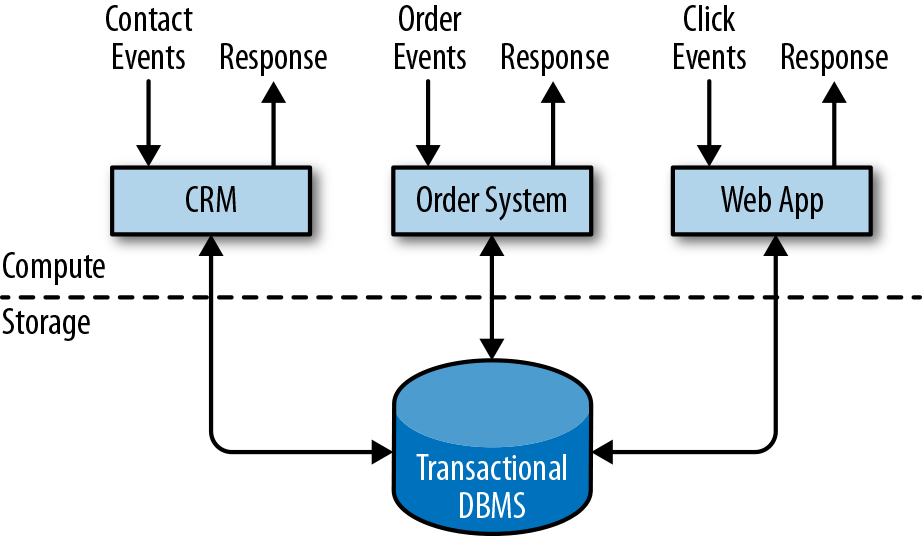
\includegraphics{images/spaf_0101.png}
\caption{传统架构}
\end{figure}

应用程序通常连接到外部服务或直接面向用户,并持续处理传入的事件,如网站上的订单,电子邮件或点击。处理事件时,应用程序将会读取远程数据库的状态,或者通过运行事务来更新它。通常,一个数据库系统可以服务于多个应用程序,它们有时会访问相同的数据库或表。

当应用程序需要扩展时,这样的设计可能会导致问题。由于多个应用程序可能会同时用到相同的数据表示,或者共享相同的基础设施,因此想要更改表的结构或扩展数据库,就需要仔细的规划和大量的工作。克服紧耦合应用程序的最新方法是微服务设计模式。微服务被设计为小型、完备且独立的应用程序。他们遵循UNIX的理念,即``只做一件事并且把它做好''。通过将几个微服务相互连接来构建更复杂的应用程序,这些微服务仅通过标准化接口(例如RESTful
HTTP连接)进行通信。由于微服务严格地彼此分离并且仅通过明确定义的接口进行通信,因此每个微服务都可以用不同技术栈来实现,包括编程语言、类库和数据存储。微服务和所有必需的软件和服务通常捆绑在一起并部署在独立的容器中。下图描绘了一种微服务架构。

\begin{figure}
\centering
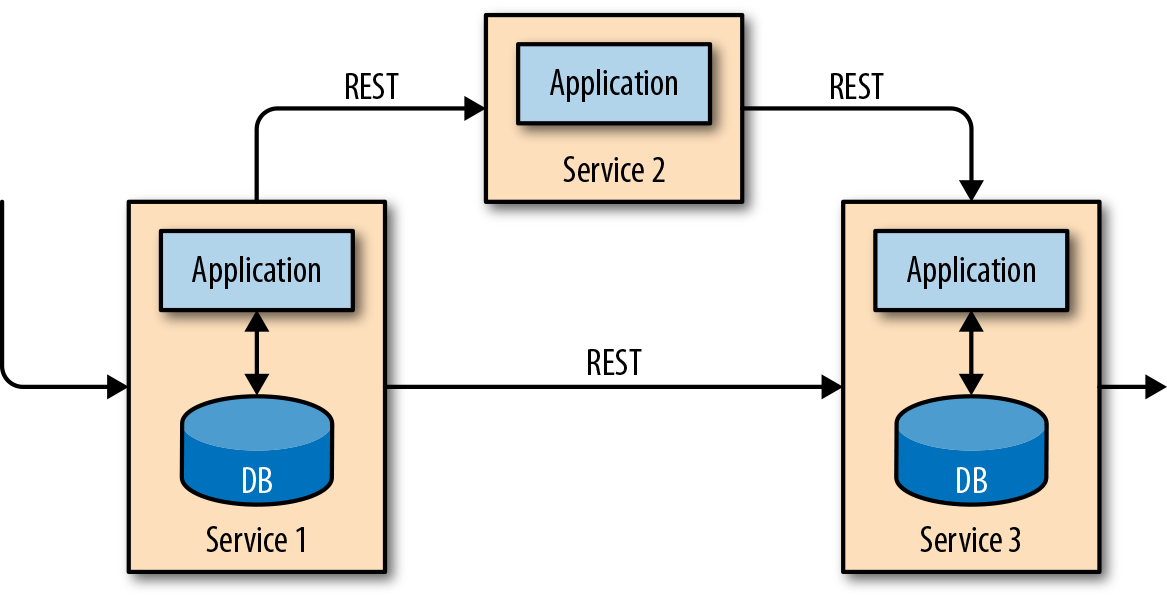
\includegraphics{images/spaf_0102.png}
\caption{微服务架构}
\end{figure}

\hypertarget{ux5206ux6790ux5904ux7406}{%
\subsection{分析处理}\label{ux5206ux6790ux5904ux7406}}

大量数据存储在公司的各种事务数据库系统中,它们可以为公司业务运营提供宝贵的参考意见。例如,分析订单处理系统的数据,可以获得销量随时间的增长曲线;可以识别延迟发货的原因;还可以预测未来的销量以便提前调整库存。但是,事务数据通常分布在多个数据库中,它们往往汇总起来联合分析时更有价值。而且,数据通常需要转换为通用格式。

所以我们一般不会直接在事务数据库上运行分析查询,而是复制数据到数据仓库。数据仓库是对工作负载进行分析和查询的专用数据存储。为了填充数据仓库,需要将事务数据库系统管理的数据复制过来。将数据复制到数据仓库的过程称为extract-transform-load(ETL)。
ETL过程从事务数据库中提取数据,将其转换为某种通用的结构表示,可能包括验证,值的规范化,编码,重复数据删除(去重)和模式转换,最后将其加载到分析数据库中。
ETL过程可能非常复杂,并且通常需要技术复杂的解决方案来满足性能要求。
ETL过程需要定期运行以保持数据仓库中的数据同步。

将数据导入数据仓库后,可以查询和分析数据。通常,在数据仓库上执行两类查询。第一种类型是定期报告查询,用于计算与业务相关的统计信息,比如收入、用户增长或者输出的产量。这些指标汇总到报告中,帮助管理层评估业务的整体健康状况。第二种类型是即席查询,旨在提供特定问题的答案并支持关键业务决策,例如收集统计在投放商业广告上的花费,和获取的相应收入,以评估营销活动的有效性。两种查询由批处理方式由数据仓库执行,如图所示。

\begin{figure}
\centering
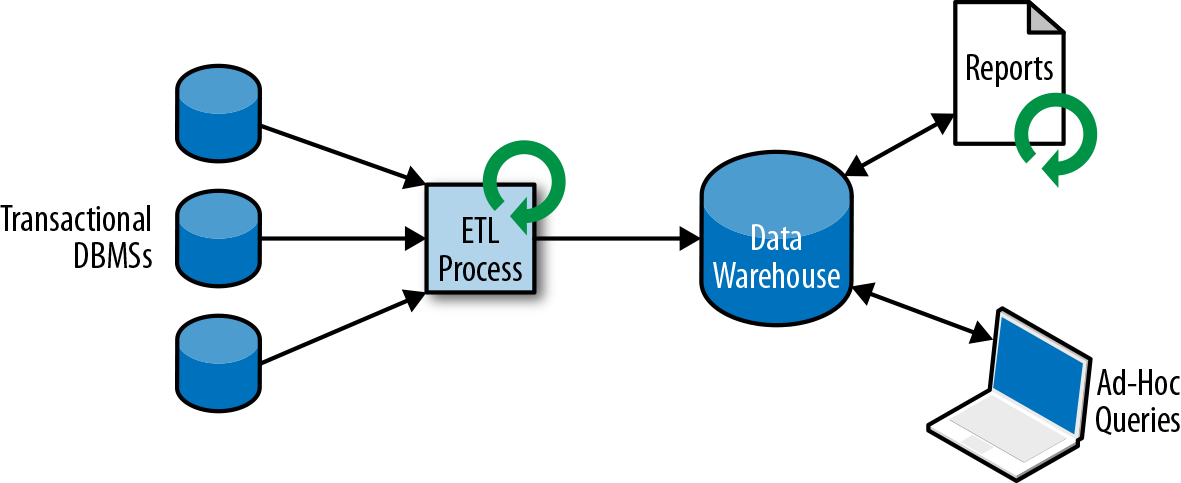
\includegraphics{images/spaf_0103.png}
\caption{在线分析}
\end{figure}

如今,Apache
Hadoop生态系统的组件,已经是许多企业IT基础架构中不可或缺的组成部分。现在的做法不是直接将所有数据都插入关系数据库系统,而是将大量数据(如日志文件,社交媒体或Web点击日志)写入Hadoop的分布式文件系统(HDFS)、S3或其他批量数据存储库,如Apache
HBase,以较低的成本提供大容量存储容量。驻留在此类存储系统中的数据可以通过SQL-on-Hadoop引擎查询和处理,例如Apache
Hive,Apache Drill或Apache
Impala。但是,基础结构与传统数据仓库架构基本相同。

\hypertarget{ux6709ux72b6ux6001ux7684ux6d41ux5f0fux5904ux7406-1}{%
\section{有状态的流式处理}\label{ux6709ux72b6ux6001ux7684ux6d41ux5f0fux5904ux7406-1}}

日常生活中,所有数据都是作为连续的事件流创建的。比如网站或者移动应用中的用户交互动作,订单的提交,服务器日志或传感器测量数据:所有这些都是事件流。实际上,很少有应用场景,能一次性地生成所需要的完整(有限)数据集。实际应用中更多的是无限事件流。有状态的流处理就是用于处理这种无限事件流的应用程序设计模式,在公司的IT基础设施中有广泛的应用场景。在我们讨论其用例之前,我们将简要介绍有状态流处理的工作原理。

如果我们想要无限处理事件流,并且不愿意繁琐地每收到一个事件就记录一次,那这样的应用程序就需要是有状态的,也就是说能够存储和访问中间数据。当应用程序收到一个新事件时,它可以从状态中读取数据,或者向该状态写入数据,总之可以执行任何计算。原则上讲,我们可以在各种不同的地方存储和访问状态,包括程序变量(内存)、本地文件,还有嵌入式或外部数据库。

Apache
Flink将应用程序状态,存储在内存或者嵌入式数据库中。由于Flink是一个分布式系统,因此需要保护本地状态以防止在应用程序或计算机故障时数据丢失。
Flink通过定期将应用程序状态的一致性检查点(check
point)写入远程且持久的存储,来保证这一点。状态、状态一致性和Flink的检查点将在后面的章节中更详细地讨论,但是,现在,下图显示了有状态的流式Flink应用程序。

\begin{figure}
\centering
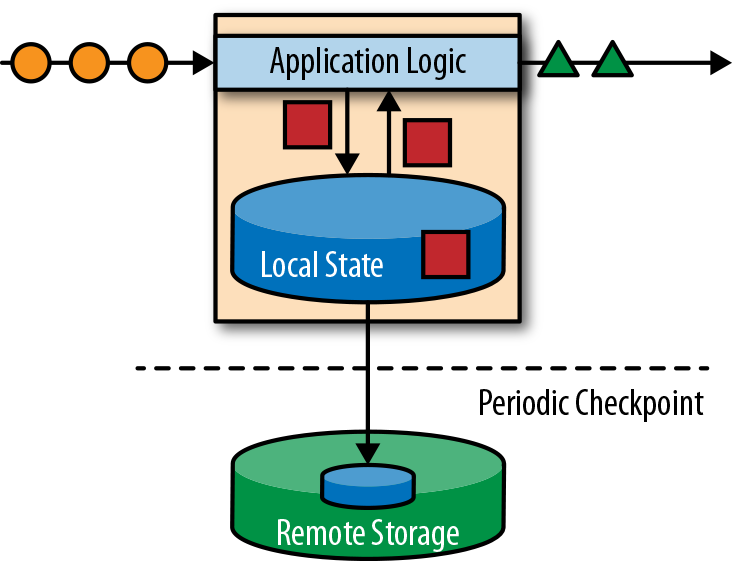
\includegraphics{images/spaf_0104.png}
\caption{有状态的流式处理}
\end{figure}

有状态的流处理应用程序,通常从事件日志中提取输入事件。事件日志就用来存储和分发事件流。事件被写入持久的仅添加(append-only)日志,这意味着无法更改写入事件的顺序。写入事件日志的流,可以被相同或不同的消费者多次读取。由于日志的仅附加(append-only)属性,事件始终以完全相同的顺序发布给所有消费者。现在已有几种事件日志系统,其中Apache
Kafka是最受欢迎的,可以作为开源软件使用,或者是云计算提供商提供的集成服务。

在Flink上运行的有状态的流处理应用程序,是很有意思的一件事。在这个架构中,事件日志会按顺序保留输入事件,并且可以按确定的顺序重播它们。如果发生故障,Flink将从先前的检查点(check
point)恢复其状态,并重置事件日志上的读取位置,这样就可以恢复整个应用。应用程序将重放(并快进)事件日志中的输入事件,直到它到达流的尾部。此技术一般用于从故障中恢复,但也可用于更新应用程序、修复bug或者修复以前发出的结果,另外还可以用于将应用程序迁移到其他群集,或使用不同的应用程序版本执行A
/ B测试。

如前所述,有状态的流处理是一种通用且灵活的设计架构,可用于许多不同的场景。在下文中,我们提出了三类通常使用有状态流处理实现的应用程序:(1)事件驱动应用程序,(2)数据管道应用程序,以及(3)数据分析应用程序。

我们将应用程序分类描述,是为了强调有状态流处理适用于多种业务场景;而实际的应用中,往往会具有以上多种情况的特征。

\hypertarget{ux4e8bux4ef6ux9a71ux52a8ux5e94ux7528ux7a0bux5e8f}{%
\subsection{事件驱动应用程序}\label{ux4e8bux4ef6ux9a71ux52a8ux5e94ux7528ux7a0bux5e8f}}

事件驱动的应用程序是有状态的流应用程序,它们使用特定的业务逻辑来提取事件流并处理事件。根据业务逻辑,事件驱动的应用程序可以触发诸如发送警报、或电子邮件之类的操作,或者将事件写入向外发送的事件流以供另一个应用程序使用。

事件驱动应用程序的典型场景包括:

\begin{itemize}
\tightlist
\item
  实时推荐(例如,在客户浏览零售商网站时推荐产品)
\item
  行为模式检测或复杂事件处理(例如,用于信用卡交易中的欺诈检测)
\item
  异常检测(例如,检测侵入计算机网络的尝试)
\end{itemize}

事件驱动应用程序是微服务的演变。它们通过事件日志而不是REST调用进行通信,并将应用程序数据保存为本地状态,而不是将其写入外部数据存储区(例如关系数据库或键值数据库)。下图显示了由事件驱动的流应用程序组成的服务架构。

\begin{figure}
\centering
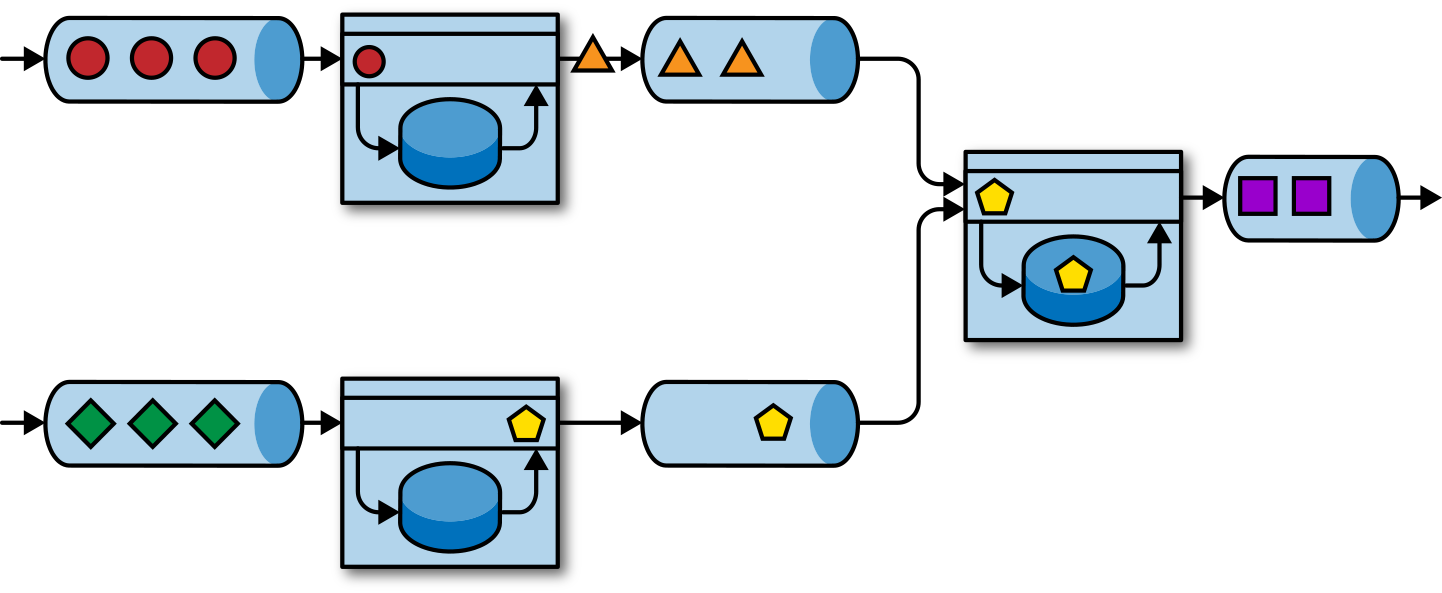
\includegraphics{images/spaf_0105.png}
\caption{事件驱动的流应用程序}
\end{figure}

上图中的应用程序通过事件日志连接。一个应用程序将其输出发送到事件日志通道(kafka),另一个应用程序使用其他应用程序发出的事件。事件日志通道将发送者和接收者分离,并提供异步、非阻塞的事件传输。每个应用程序都可以是有状态的,并且可以本地管理自己的状态而无需访问外部数据存储。应用程序也可以单独处理和扩展。

与事务性应用程序或微服务相比,事件驱动的应用程序具有多种优势。与读写远程数据库相比,本地状态访问提供了非常好的性能。扩展性和容错性都由流处理器来保证,并且以事件日志作为输入源,应用程序的整个输入数据可以可靠地存储,并且可以确定性地重放。此外,Flink可以将应用程序的状态重置为先前的保存点(save
point),从而可以在不丢失状态的情况下更新或重新扩展应用程序。

事件驱动的应用程序对运行它们的流处理器有很高的要求,并不是所有流处理器都适合运行事件驱动的应用程序。
API的表现力,以及对状态处理和事件时间支持的程度,决定了可以实现和执行的业务逻辑。这方面取决于流处理器的API,主要看它能提供什么样的状态类型,以及它对事件时间处理的支持程度。此外,精确一次(exactly-once)的状态一致性和扩展应用程序的能力是事件驱动应用程序的基本要求。
Apache Flink符合所有的这些要求,是运行此类应用程序的一个非常好的选择。

\hypertarget{ux6570ux636eux7ba1ux9053}{%
\subsection{数据管道}\label{ux6570ux636eux7ba1ux9053}}

当今的IT架构包括许多不同的数据存储,例如关系型数据库和专用数据库系统、事件日志、分布式文件系统,内存中的缓存和搜索索引。所有这些系统都以不同的格式和数据结构存储数据,为其特定的访问模式提供最佳性能。公司通常将相同的数据存储在多个不同的系统中,以提高数据访问的性能。例如,网上商店中提供的产品的信息,可以存储在交易数据库中,同时也存储在缓存(如redis)和搜索索引(如ES)中。由于数据的这种复制,数据存储必须保持同步。

在不同存储系统中同步数据的传统方法是定期ETL作业。但是,它们不能满足当今许多场景的延迟要求。另一种方法是使用事件日志(event
log)来发布更新。更新将写入事件日志并由事件日志分发。日志的消费者获取到更新之后,将更新合并到受影响的数据存储中。根据使用情况,传输的数据可能需要标准化、使用外部数据进行扩展,或者在目标数据存储提取之前进行聚合。

以较低的延迟,来提取、转换和插入数据是有状态流处理应用程序的另一个常见应用场景。这种类型的应用程序称为数据管道(data
pipeline)。数据管道必须能够在短时间内处理大量数据。操作数据管道的流处理器还应具有许多源(source)和接收器(sink)的连接器,以便从各种存储系统读取数据并将数据写入各种存储系统。当然,同样地,Flink完成了所有这些功能。

\hypertarget{ux6d41ux5206ux6790}{%
\subsection{流分析}\label{ux6d41ux5206ux6790}}

ETL作业定期将数据导入数据存储区,数据的处理是由即席查询(用户自定义查询)或设定好的通常查询来做的。无论架构是基于数据仓库还是基于Hadoop生态系统的组件,这都是批处理。多年来最好的处理方式就是,定期将数据加载到数据分析系统中,但它给分析管道带了的延迟相当大,而且无法避免。

根据设定好的时间间隔,可能需要数小时或数天才能将数据点包含在报告中。我们前面已经提到,数据管道可以实现低延迟的ETL,所以在某种程度上,可以通过使用数据管道将数据导入存储区来减少延迟。但是,即使持续不停地进行ETL操作,在用查询来处理事件之前总会有延迟。虽然这种延迟在过去可能是可以接受的,但是今天的应用程序,往往要求必须能够实时收集数据,并立即对其进行操作(例如,在手机游戏中去适应不断变化的条件,或者在电商网站中提供个性化的用户体验)。

流式分析应用程序不是等待定期触发,而是连续地提取事件流,并且通过纳入最新事件来更新其计算结果,这个过程是低延迟的。这有些类似于数据库中用于更新视图(views)的技术。通常,流应用程序将其结果存储在支持更新的外部数据存储中,例如数据库或键值(key-value)存储。流分析应用程序的实时更新结果可用于驱动监控仪表板(dashboard)应用程序,如下图所示。

\begin{figure}
\centering
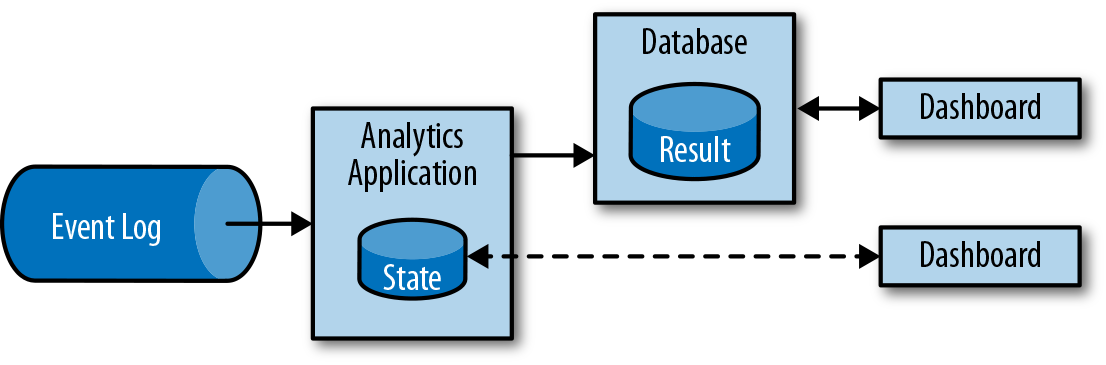
\includegraphics{images/spaf_0106.png}
\caption{仪表盘}
\end{figure}

流分析应用程序最大的优势就是,将每个事件纳入到分析结果所需的时间短得多。除此之外,流分析应用程序还有另一个不太明显的优势。传统的分析管道由几个独立的组件组成,例如ETL过程、存储系统、对于基于Hadoop的环境,还包括用于触发任务(jobs)的数据处理和调度程序。相比之下,如果我们运行一个有状态流应用程序,那么流处理器就会负责所有这些处理步骤,包括事件提取、带有状态维护的连续计算以及更新结果。此外,流处理器可以从故障中恢复,并且具有精确一次(exactly-once)的状态一致性保证,还可以调整应用程序的计算资源。像Flink这样的流处理器还支持事件时间(event-time)处理,这可以保证产生正确和确定的结果,并且能够在很短的时间内处理大量数据。

流分析应用程序通常用于:

\begin{itemize}
\tightlist
\item
  监控手机网络的质量分析
\item
  移动应用中的用户行为
\item
  实时数据的即席分析
\end{itemize}

虽然我们不在此处介绍,但Flink还提供对流上的分析SQL查询的支持。

\hypertarget{ux5f00ux6e90ux6d41ux5904ux7406ux7684ux6f14ux8fdb}{%
\section{开源流处理的演进}\label{ux5f00ux6e90ux6d41ux5904ux7406ux7684ux6f14ux8fdb}}

数据流处理并不是一项新技术。一些最初的研究原型和商业产品可以追溯到20世纪90年代(1990s)。然而,在很大程度上,过去采用的流处理技术是由成熟的开源流处理器驱动的。如今,分布式开源流处理器在不同行业的许多企业中,处理着核心业务应用,比如电商、社交媒体、电信、游戏和银行等。开源软件是这一趋势的主要驱动力,主要原因有两个:

\begin{itemize}
\tightlist
\item
  开源流处理软件是大家每一个人都可以评估和使用的产品。
\item
  由于许多开源社区的努力,可扩展流处理技术正在迅速成熟和发展。
\end{itemize}

仅仅一个Apache软件基金会就支持了十几个与流处理相关的项目。新的分布式流处理项目不断进入开源阶段,并不断增加新的特性和功能。开源社区不断改进其项目的功能,并正在推动流处理的技术边界。我们将简要介绍一下过去,看看开源流处理的起源和今天的状态。

第一代分布式开源流处理器(2011)专注于具有毫秒延迟的事件处理,并提供了在发生故障时防止事件丢失的保证。这些系统具有相当低级的API,并且对于流应用程序的准确性和结果的一致性,不提供内置支持,因为结果会取决于到达事件的时间和顺序。另外,即使事件没有丢失,也可能不止一次地处理它们。与批处理器相比,第一代开源流处理器牺牲了结果准确性,用来获得更低的延迟。为了让当时的数据处理系统,可以同时提供快速和准确的结果,人们设计了所谓的lambda架构,如图所示。

\begin{figure}
\centering
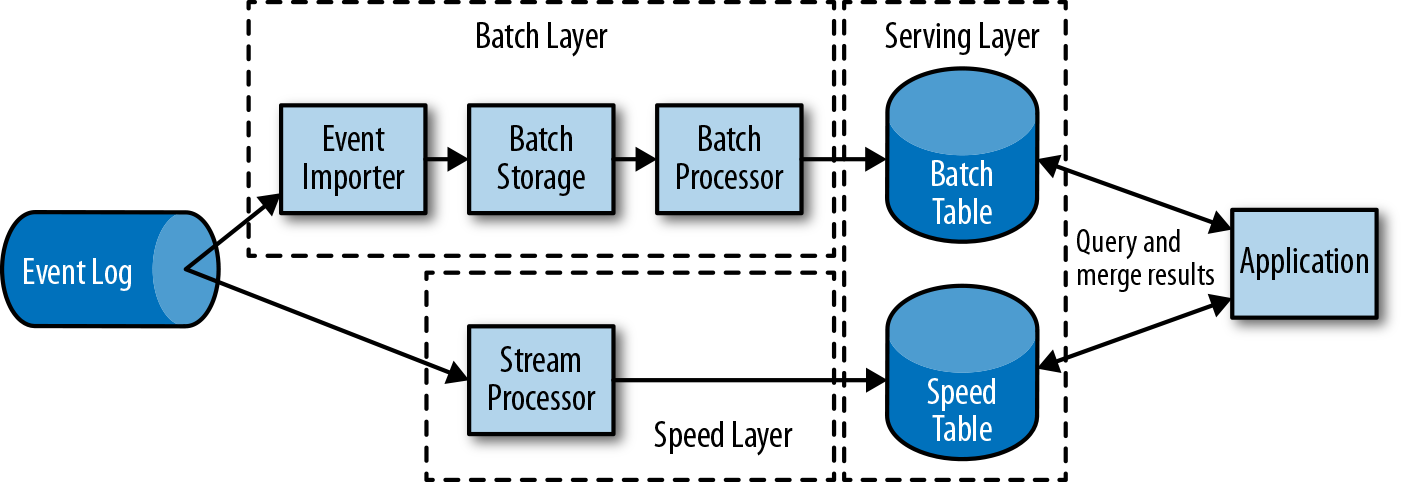
\includegraphics{images/spaf_0107.png}
\caption{lambda架构}
\end{figure}

lambda架构增强了传统的批处理架构,其``快速层''(speed
layer)由低延迟的流处理器来支持。数据到达之后由流处理器提取出来,并写入批处理存储。流处理器近乎实时地计算近似结果并将它们写入``快速表''(speed
table)。批处理器定期处理批量存储中的数据,将准确的结果写入批处理表,并从速度表中删除相应的不准确结果。应用程序会合并快速表中的近似结果和批处理表中的准确结果,然后消费最终的结果。

lambda架构现在已经不再是最先进的,但仍在许多地方使用。该体系结构的最初目标是改善原始批处理分析体系结构的高延迟。但是,它有一些明显的缺点。首先,它需要对一个应用程序,做出两个语义上等效的逻辑实现,用于两个独立的、具有不同API的处理系统。其次,流处理器计算的结果只是近似的。第三,lambda架构很难建立和维护。

通过在第一代基础上进行改进,下一代分布式开源流处理器(2013)提供了更好的故障保证,并确保在发生故障时,每个输入记录仅对结果产生一次影响(exactly
-once)。此外,编程API从相当低级的操作符接口演变为高级API。但是,一些改进(例如更高的吞吐量和更好的故障保证)是以将处理延迟从毫秒增加到几秒为代价的。此外,结果仍然取决于到达事件的时间和顺序。

第三代分布式开源流处理器(2015)解决了结果对到达事件的时间和顺序的依赖性。结合精确一次(exactly-once)的故障语义,这一代系统是第一个具有计算一致性和准确结果的开源流处理器。通过基于实际数据来计算结果(``重演''数据),这些系统还能够以与``实时''数据相同的方式处理历史数据。另一个改进是解决了延迟/吞吐量无法同时保证的问题。先前的流处理器仅能提供高吞吐量或者低延迟(其中之一),而第三代系统能够同时提供这两个特性。这一代的流处理器使得lambda架构过时了。当然,这一代流处理以flink为代表。

除了目前讨论的特性,例如容错、性能和结果准确性之外,流处理器还不断添加新的操作功能,例如高可用性设置,与资源管理器(如YARN或Kubernetes)的紧密集成,以及能够动态扩展流应用程序。其他功能包括:支持升级应用程序代码,或将作业迁移到其他群集或新版本的流处理器,而不会丢失当前状态。

\hypertarget{flinkux7b80ux4ecb}{%
\section{Flink简介}\label{flinkux7b80ux4ecb}}

Apache
Flink是第三代分布式流处理器,它拥有极富竞争力的功能。它提供准确的大规模流处理,具有高吞吐量和低延迟。特别的是,以下功能使Flink脱颖而出:

\begin{itemize}
\tightlist
\item
  事件时间(event-time)和处理时间(processing-tme)语义。即使对于无序事件流,事件时间(event-time)语义仍然能提供一致且准确的结果。而处理时间(processing-time)语义可用于具有极低延迟要求的应用程序。
\item
  精确一次(exactly-once)的状态一致性保证。
\item
  每秒处理数百万个事件,毫秒级延迟。
  Flink应用程序可以扩展为在数千个核(cores)上运行。
\item
  分层API,具有不同的权衡表现力和易用性。本书介绍了DataStream
  API和过程函数(process
  function),为常见的流处理操作提供原语,如窗口和异步操作,以及精确控制状态和时间的接口。本书不讨论Flink的关系API,SQL和LINQ风格的Table
  API。
\item
  连接到最常用的存储系统,如Apache Kafka,Apache
  Cassandra,Elasticsearch,JDBC,Kinesis和(分布式)文件系统,如HDFS和S3。
\item
  由于其高可用的设置(无单点故障),以及与Kubernetes,YARN和Apache
  Mesos的紧密集成,再加上从故障中快速恢复和动态扩展任务的能力,Flink能够以极少的停机时间7*24全天候运行流应用程序。
\item
  能够更新应用程序代码并将作业(jobs)迁移到不同的Flink集群,而不会丢失应用程序的状态。
\item
  详细且可自定义的系统和应用程序指标集合,以提前识别问题并对其做出反应。
\item
  最后但同样重要的是,Flink也是一个成熟的批处理器。
\end{itemize}

除了这些功能之外,Flink还是一个非常易于开发的框架,因为它易于使用的API。嵌入式执行模式,可以在单个JVM进程中启动应用程序和整个Flink系统,这种模式一般用于在IDE中运行和调试Flink作业。在开发和测试Flink应用程序时,此功能非常有用。

\hypertarget{ux7f16ux5199ux7b2cux4e00ux4e2aflinkux7a0bux5e8f}{%
\section{编写第一个Flink程序}\label{ux7f16ux5199ux7b2cux4e00ux4e2aflinkux7a0bux5e8f}}

\hypertarget{ux5728ideaux4e2dux7f16ux5199flinkux7a0bux5e8f}{%
\subsection{在IDEA中编写Flink程序}\label{ux5728ideaux4e2dux7f16ux5199flinkux7a0bux5e8f}}

\begin{enumerate}
\def\labelenumi{\arabic{enumi}.}
\tightlist
\item
  使用Intellij IDEA创建一个Maven新项目
\item
  勾选Create from archetype,然后点击Add Archetype按钮
\item
  GroupId中输入org.apache.flink,ArtifactId中输入flink-quickstart-java,Version中输入Flink的版本号,然后点击OK
\item
  点击向右箭头,出现下拉列表,选中flink-quickstart-java:版本号,点击Next
\item
  Name中输入FlinkTutorial,GroupId中输入com.atguigu,ArtifactId中输入FlinkTutorial,点击Next
\item
  最好使用IDEA默认的Maven工具:Bundled(Maven
  3),点击Finish,等待一会儿,项目就创建好了
\end{enumerate}

编写\texttt{WordCount.java}程序

\begin{Shaded}
\begin{Highlighting}[]
\KeywordTok{public} \KeywordTok{class}\NormalTok{ WordCount \{}

    \KeywordTok{public} \DataTypeTok{static} \DataTypeTok{void} \FunctionTok{main}\NormalTok{(}\BuiltInTok{String}\NormalTok{[] args) }\KeywordTok{throws} \BuiltInTok{Exception}\NormalTok{ \{}
        \DataTypeTok{final}\NormalTok{ StreamExecutionEnvironment env = StreamExecutionEnvironment.}\FunctionTok{getExecutionEnvironment}\NormalTok{();}
\NormalTok{        env.}\FunctionTok{setParallelism}\NormalTok{(}\DecValTok{1}\NormalTok{);}

\NormalTok{        DataStream\textless{}}\BuiltInTok{String}\NormalTok{\textgreater{} stream = env.}\FunctionTok{fromElements}\NormalTok{(}\StringTok{"Hello World"}\NormalTok{, }\StringTok{"Hello World"}\NormalTok{);}

\NormalTok{        stream}
\NormalTok{                .}\FunctionTok{flatMap}\NormalTok{(}\KeywordTok{new} \FunctionTok{Tokenizer}\NormalTok{())}
\NormalTok{                .}\FunctionTok{keyBy}\NormalTok{(r {-}\textgreater{} r.}\FunctionTok{f0}\NormalTok{)}
\NormalTok{                .}\FunctionTok{sum}\NormalTok{(}\DecValTok{1}\NormalTok{)}
\NormalTok{                .}\FunctionTok{print}\NormalTok{();}

\NormalTok{        env.}\FunctionTok{execute}\NormalTok{(}\StringTok{"单词计数"}\NormalTok{);}
\NormalTok{    \}}

    \KeywordTok{public} \DataTypeTok{static} \KeywordTok{class}\NormalTok{ Tokenizer }\KeywordTok{implements}\NormalTok{ FlatMapFunction\textless{}}\BuiltInTok{String}\NormalTok{, Tuple2\textless{}}\BuiltInTok{String}\NormalTok{, }\BuiltInTok{Integer}\NormalTok{\textgreater{}\textgreater{} \{}
        \AttributeTok{@Override}
        \KeywordTok{public} \DataTypeTok{void} \FunctionTok{flatMap}\NormalTok{(}\BuiltInTok{String}\NormalTok{ value, Collector\textless{}Tuple2\textless{}}\BuiltInTok{String}\NormalTok{, }\BuiltInTok{Integer}\NormalTok{\textgreater{}\textgreater{} out) }\KeywordTok{throws} \BuiltInTok{Exception}\NormalTok{ \{}
            \BuiltInTok{String}\NormalTok{[] stringList = value.}\FunctionTok{split}\NormalTok{(}\StringTok{"}\SpecialCharTok{\textbackslash{}\textbackslash{}}\StringTok{s"}\NormalTok{);}
            \KeywordTok{for}\NormalTok{ (}\BuiltInTok{String}\NormalTok{ s : stringList) \{}
\NormalTok{                out.}\FunctionTok{collect}\NormalTok{(Tuple2.}\FunctionTok{of}\NormalTok{(s, }\DecValTok{1}\NormalTok{));}
\NormalTok{            \}}
\NormalTok{        \}}
\NormalTok{    \}}
\NormalTok{\}}
\end{Highlighting}
\end{Shaded}

\hypertarget{ux4e0bux8f7dflinkux8fd0ux884cux65f6ux73afux5883ux63d0ux4ea4jarux5305ux7684ux8fd0ux884cux65b9ux5f0f}{%
\subsection{下载Flink运行时环境,提交Jar包的运行方式}\label{ux4e0bux8f7dflinkux8fd0ux884cux65f6ux73afux5883ux63d0ux4ea4jarux5305ux7684ux8fd0ux884cux65b9ux5f0f}}

先下载压缩包,然后进行解压。然后进入文件夹。

\begin{Shaded}
\begin{Highlighting}[]
\NormalTok{$ }\ExtensionTok{./bin/start{-}cluster.sh}
\end{Highlighting}
\end{Shaded}

可以打开Flink WebUI查看集群状态:http://localhost:8081

在IDEA中使用maven package打包。

提交打包好的JAR包:

\begin{Shaded}
\begin{Highlighting}[]
\NormalTok{$ }\ExtensionTok{./bin/flink}\NormalTok{ run 打包好的JAR包的绝对路径}
\end{Highlighting}
\end{Shaded}

停止Flink集群

\begin{Shaded}
\begin{Highlighting}[]
\NormalTok{$ }\ExtensionTok{./bin/stop{-}cluster.sh}
\end{Highlighting}
\end{Shaded}

查看标准输出日志的位置,在log文件夹中。

\begin{Shaded}
\begin{Highlighting}[]
\NormalTok{$ }\BuiltInTok{cd}\NormalTok{ log/}
\end{Highlighting}
\end{Shaded}

\hypertarget{ux6d41ux5904ux7406ux57faux7840}{%
\chapter{流处理基础}\label{ux6d41ux5904ux7406ux57faux7840}}

\hypertarget{ux6570ux636eux6d41ux7f16ux7a0b}{%
\section{数据流编程}\label{ux6570ux636eux6d41ux7f16ux7a0b}}

在我们深入研究流处理的基础知识之前,让我们来看看在数据流程编程的背景和使用的术语。

\hypertarget{ux6570ux636eux6d41ux56fe}{%
\subsection{数据流图}\label{ux6570ux636eux6d41ux56fe}}

顾名思义,数据流程序描述了数据如何在算子之间流动。数据流程序通常表示为有向图,其中节点称为算子,用来表示计算,边表示数据之间的依赖性。算子是数据流程序的基本功能单元。他们从输入消耗数据,对它们执行计算,并生成数据输出用于进一步处理。一个数据流图必须至少有一个数据源和一个数据接收器。

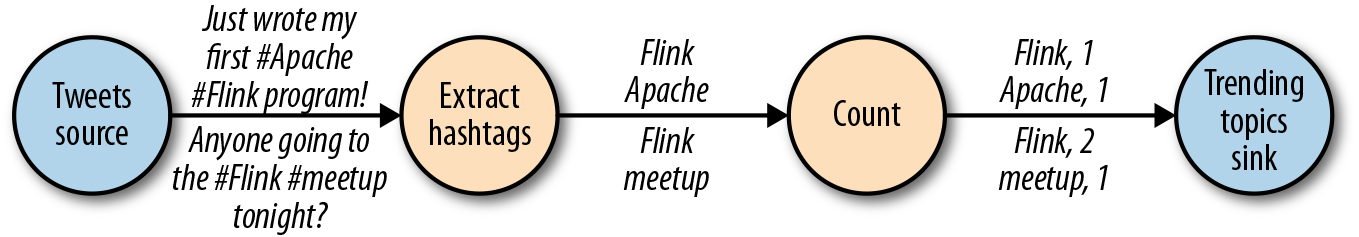
\includegraphics{images/spaf_0201.png}

像上图中的数据流图被称为逻辑流图,因为它们表示了计算逻辑的高级视图。为了执行一个数据流程序,Flink会将逻辑流图转换为物理数据流图,详细说明程序的执行方式。例如,如果我们使用分布式处理引擎,每个算子在不同的物理机器可能有几个并行的任务运行。图2-2显示了图2-1逻辑图的物理数据流图。而在逻辑数据流图中节点表示算子,在物理数据流图中,节点是任务。``Extract
hashtags''和``Count''算子有两个并行算子任务,每个算子任务对输入数据的子集执行计算。

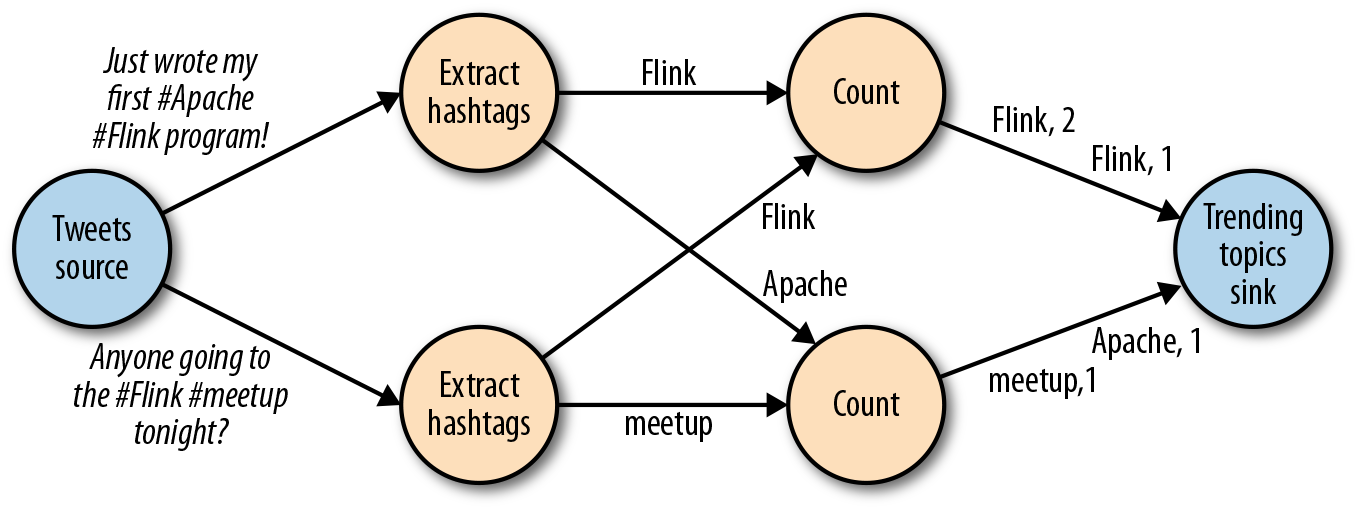
\includegraphics{images/spaf_0202.png}

\hypertarget{ux6570ux636eux5e76ux884cux548cux4efbux52a1ux5e76ux884c}{%
\subsection{数据并行和任务并行}\label{ux6570ux636eux5e76ux884cux548cux4efbux52a1ux5e76ux884c}}

我们可以以不同方式利用数据流图中的并行性。第一,我们可以对输入数据进行分区,并在数据的子集上并行执行具有相同算子的任务并行。这种类型的并行性被称为数据并行性。数据并行是有用的,因为它允许处理大量数据,并将计算分散到不同的计算节点上。第二,我们可以将不同的算子在相同或不同的数据上并行执行。这种并行性称为任务并行性。使用任务并行性,我们可以更好地利用计算资源。

\hypertarget{ux6570ux636eux4ea4ux6362ux7b56ux7565}{%
\subsection{数据交换策略}\label{ux6570ux636eux4ea4ux6362ux7b56ux7565}}

数据交换策略定义了在物理执行流图中如何将数据分配给任务。数据交换策略可以由执行引擎自动选择,具体取决于算子的语义或我们明确指定的语义。在这里,我们简要回顾一些常见的数据交换策略,如图2-3所示。

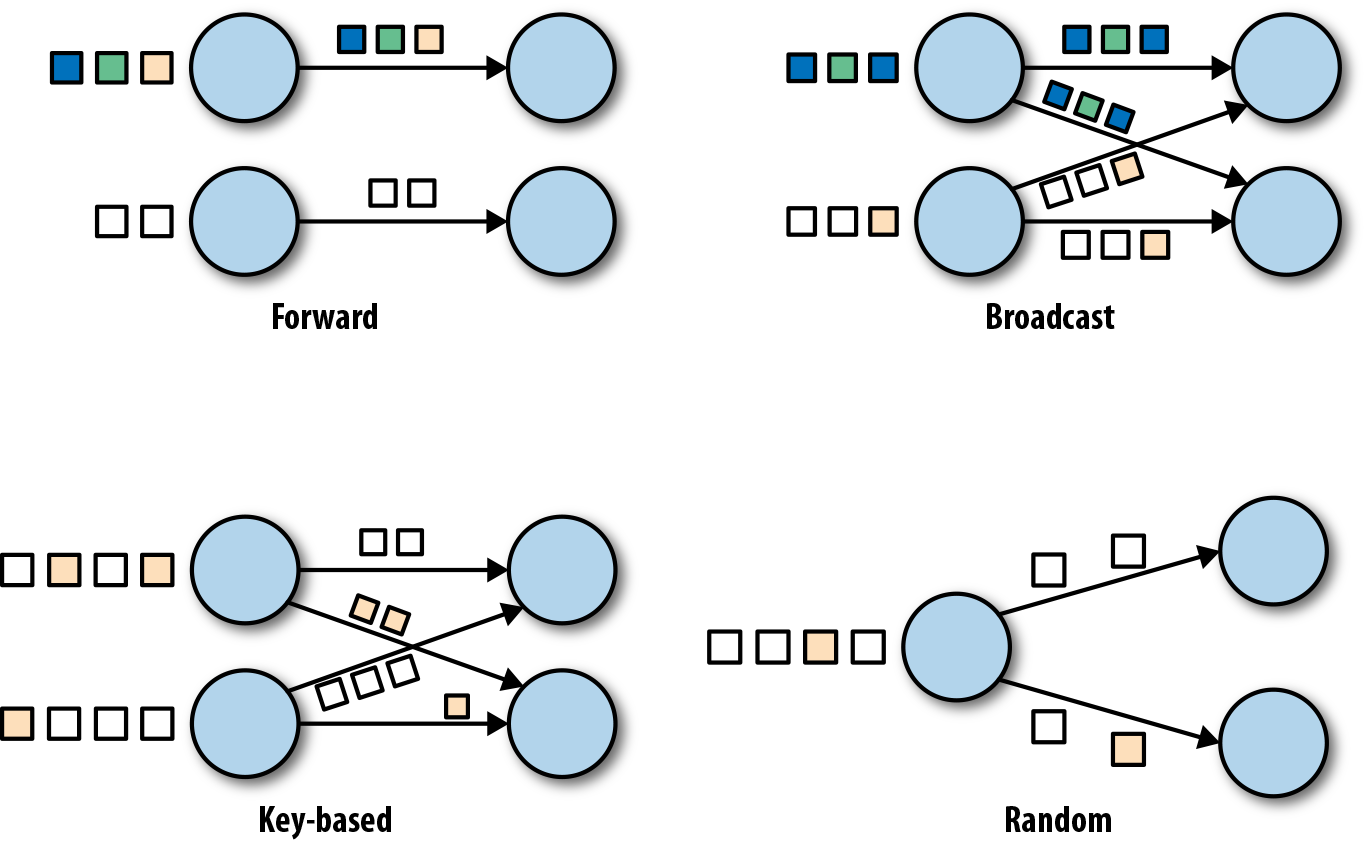
\includegraphics{images/spaf_0203.png}

\begin{itemize}
\tightlist
\item
  前向策略将数据从一个任务发送到接收任务。如果两个任务都位于同一台物理计算机上(这通常由任务调度器确保),这种交换策略可以避免网络通信。
\item
  广播策略将所有数据发送到算子的所有的并行任务上面去。因为这种策略会复制数据和涉及网络通信,所以代价相当昂贵。
\item
  基于键控的策略通过Key值(键)对数据进行分区保证具有相同Key的数据将由同一任务处理。在图2-2中,输出``Extract
  hashtags''算子使用键来分区(hashtag),以便count算子的任务可以正确计算每个\texttt{\#}标签的出现次数。
\item
  随机策略统一将数据分配到算子的任务中去,以便均匀地将负载分配到不同的计算任务。
\end{itemize}

\hypertarget{ux5e76ux884cux5904ux7406ux6d41ux6570ux636e}{%
\section{并行处理流数据}\label{ux5e76ux884cux5904ux7406ux6d41ux6570ux636e}}

既然我们熟悉了数据流编程的基础知识,现在是时候看看这些概念如何应用于并行的处理数据流了。但首先,让我们定义术语数据流:数据流是一个可能无限的事件序列。

数据流中的事件可以表示监控数据,传感器测量数据,信用卡交易数据,气象站观测数据,在线用户交互数据,网络搜索数据等。在本节中,我们将学习如何并行处理无限流,使用数据流编程范式。

\hypertarget{ux5ef6ux8fdfux548cux541eux5410ux91cf}{%
\subsection{延迟和吞吐量}\label{ux5ef6ux8fdfux548cux541eux5410ux91cf}}

流处理程序不同与批处理程序。在评估性能时,要求也有所不同。对于批处理程序,我们通常关心一个作业的总的执行时间,或我们的处理引擎读取输入所需的时间,执行计算,并回写结果。由于流处理程序是连续运行的,输入可能是无界的,所以数据流处理中没有总执行时间的概念。
相反,流处理程序必须尽可能快的提供输入数据的计算结果。我们使用延迟和吞吐量来表征流处理的性能要求。

\hypertarget{ux5ef6ux8fdf}{%
\subsection{延迟}\label{ux5ef6ux8fdf}}

延迟表示处理事件所需的时间。它是接收事件和看到在输出中处理此事件的效果之间的时间间隔。要直观的理解延迟,考虑去咖啡店买咖啡。当你进入咖啡店时,可能还有其他顾客在里面。因此,你排队等候直到轮到你下订单。收银员收到你的付款并通知准备饮料的咖啡师。一旦你的咖啡准备好了,咖啡师会叫你的名字,你可以到柜台拿你的咖啡。服务延迟是从你进入咖啡店的那一刻起,直到你喝上第一口咖啡之间的时间间隔。

在数据流中,延迟是以时间为单位测量的,例如毫秒。根据应用程序,我们可能会关心平均延迟,最大延迟或百分位延迟。例如,平均延迟值为10ms意味着处理事件的平均时间在10毫秒内。或者,延迟值为95\%,10ms表示95\%的事件在10ms内处理完毕。平均值隐藏了处理延迟的真实分布,可能会让人难以发现问题。如果咖啡师在准备卡布奇诺之前用完了牛奶,你必须等到他们从供应室带来一些。虽然你可能会因为这么长时间的延迟而生气,但大多数其他客户仍然会感到高兴。

确保低延迟对于许多流应用程序来说至关重要,例如欺诈检测,系统警报,网络监控和提供具有严格服务水平协议的服务。低延迟是流处理的关键特性,它实现了我们所谓的实时应用程序。像Apache
Flink这样的现代流处理器可以提供低至几毫秒的延迟。相比之下,传统批处理程序延迟通常从几分钟到几个小时不等。在批处理中,首先需要收集事件批次,然后才能处理它们。因此,延迟是受每个批次中最后一个事件的到达时间的限制。所以自然而然取决于批的大小。真正的流处理不会引入这样的人为延迟,因此可以实现真正的低延迟。真的流模型,事件一进入系统就可以得到处理。延迟更密切地反映了在每个事件上必须进行的实际工作。

\hypertarget{ux541eux5410ux91cf}{%
\subsection{吞吐量}\label{ux541eux5410ux91cf}}

吞吐量是衡量系统处理能力的指标,也就是处理速率。也就是说,吞吐量告诉我们每个时间单位系统可以处理多少事件。重温咖啡店的例子,如果商店营业时间为早上7点至晚上7点。当天为600个客户提供了服务,它的平均吞吐量将是每小时50个客户。虽然我们希望延迟尽可能低,但我们通常也需要吞吐量尽可能高。

吞吐量以每个时间单位系统所能处理的事件数量或操作数量来衡量。值得注意的是,事件处理速率取决于事件到达的速率,低吞吐量并不一定表示性能不佳。
在流式系统中,我们通常希望确保我们的系统可以处理最大的预期事件到达的速率。也就是说,我们主要的关注点在于确定的峰值吞吐量是多少,当系统处于最大负载时性能怎么样。为了更好地理解峰值吞吐量的概念,让我们考虑一个流处理
程序没有收到任何输入的数据,因此没有消耗任何系统资源。当第一个事件进来时,它会尽可能以最小延迟立即处理。例如,如果你是第一个出现在咖啡店的顾客,在早上开门后,你将立即获得服务。理想情况下,您希望此延迟保持不变
,并且独立于传入事件的速率。但是,一旦我们达到使系统资源被完全使用的事件传入速率,我们将不得不开始缓冲事件。在咖啡店里
,午餐后会看到这种情况发生。许多人出现在同一时间,必须排队等候。在此刻,咖啡店系统已达到其峰值吞吐量,进一步增加
事件传入的速率只会导致更糟糕的延迟。如果系统继续以可以处理的速率接收数据,缓冲区可能变为不可用,数据可能会丢失。这种情况是众所周知的
作为背压,有不同的策略来处理它。

\hypertarget{ux5ef6ux8fdfux4e0eux541eux5410ux91cfux7684ux5bf9ux6bd4}{%
\subsection{延迟与吞吐量的对比}\label{ux5ef6ux8fdfux4e0eux541eux5410ux91cfux7684ux5bf9ux6bd4}}

此时,应该清楚延迟和吞吐量不是独立指标。如果事件需要在处理流水线中待上很长时间,我们不能轻易确保高吞吐量。同样,如果系统容量很小,事件将被缓冲,而且必须等待才能得到处理。

让我们重温一下咖啡店的例子来阐明一下延迟和吞吐量如何相互影响。首先,应该清楚存在没有负载时的最佳延迟。也就是说,如果你是咖啡店的唯一客户,会很快得到咖啡。然而,在繁忙时期,客户将不得不排队等待,并且会有延迟增加。另一个影响延迟和吞吐量的因素是处理事件所花费的时间或为每个客户提供服务所花费的时间。想象一下,期间圣诞节假期,咖啡师不得不为每杯咖啡画圣诞老人。这意味着准备一杯咖啡需要的时间会增加,导致每个人花费
更多的时间在等待咖啡师画圣诞老人,从而降低整体吞吐量。

那么,你可以同时获得低延迟和高吞吐量吗?或者这是一个无望的努力?我们可以降低得到咖啡的延迟
,方法是:聘请一位更熟练的咖啡师来准备咖啡。在高负载时,这种变化也会增加吞吐量,因为会在相同的时间内为更多的客户提供服务。
实现相同结果的另一种方法是雇用第二个咖啡师来利用并行性。这里的主要想法是降低延迟来增加吞吐量。当然,如果系统可以更快的执行操作,它可以在相同的时间内执行更多操作。
事实上,在流中利用并行性时也会发生这种情况。通过并行处理多个流,在同时处理更多事件的同时降低延迟。

\hypertarget{ux6570ux636eux6d41ux4e0aux7684ux64cdux4f5c}{%
\section{数据流上的操作}\label{ux6570ux636eux6d41ux4e0aux7684ux64cdux4f5c}}

流处理引擎通常提供一组内置操作:摄取(ingest),转换(transform)和输出流(output)。这些操作可以
结合到数据流图中来实现逻辑流处理程序。在本节中,我们描述最常见的流处理操作。

操作可以是无状态的或有状态的。无状态操作不保持任何内部状态。也就是说,事件的处理不依赖于过去看到的任何事件,也没有保留历史。
无状态操作很容易并行化,因为事件可以彼此独立地处理,也独立于事件到达的顺序(和事件到达顺序没有关系)。
而且,在失败的情况下,无状态操作可以是简单的重新启动并从中断处继续处理。相反,
有状态操作可能会维护之前收到的事件的信息。此状态可以通过传入事件更新,也可以用于未来事件的处理逻辑。有状态的流
处理应用程序更难以并行化和以容错的方式来运行,因为状态需要有效的进行分区和在发生故障的情况下可靠地恢复。

\hypertarget{ux6570ux636eux6444ux5165ux548cux6570ux636eux541eux5410ux91cf}{%
\subsection{数据摄入和数据吞吐量}\label{ux6570ux636eux6444ux5165ux548cux6570ux636eux541eux5410ux91cf}}

数据摄取和数据出口操作允许流处理程序与外部系统通信。数据摄取是操作从外部源获取原始数据并将其转换为其他格式(ETL)。实现数据提取逻辑的运算符被称为数据源。数据源可以从TCP
Socket,文件,Kafka
Topic或传感器数据接口中提取数据。数据出口是以适合消费的形式产出到外部系统。执行数据出口的运算符称为数据接收器,包括文件,数据库,消息队列和监控接口。

\hypertarget{ux8f6cux6362ux7b97ux5b50}{%
\subsection{转换算子}\label{ux8f6cux6362ux7b97ux5b50}}

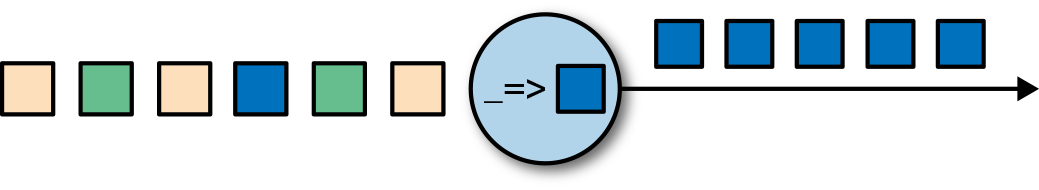
\includegraphics{images/spaf_0204.png}

转换算子是单遍处理算子,碰到一个事件处理一个事件。这些操作在使用后会消费一个事件,然后对事件数据做一些转换,产生一个新的输出流。转换逻辑可以集成在
操作符中或由UDF函数提供,如图所示图2-4。程序员编写实现自定义计算逻辑。

操作符可以接受多个输入流并产生多个输出流。他们还可以通过修改数据流图的结构要么将流分成多个流,要么将流合并为一条流。

\hypertarget{ux6edaux52a8ux805aux5408}{%
\subsection{滚动聚合}\label{ux6edaux52a8ux805aux5408}}

滚动聚合是一种聚合,例如sum,minimum和maximum,为每个输入事件不断更新。
聚合操作是有状态的,并将当前状态与传入事件一起计算以产生更新的聚合值。请注意能够有效地将当前状态与事件相结合
产生单个值,聚合函数必须是关联的和可交换的。否则,操作符必须存储完整的流数据历史。图2-5显示了最小滚动
聚合。操作符保持当前的最小值和相应地为每个传入的事件来更新最小值。

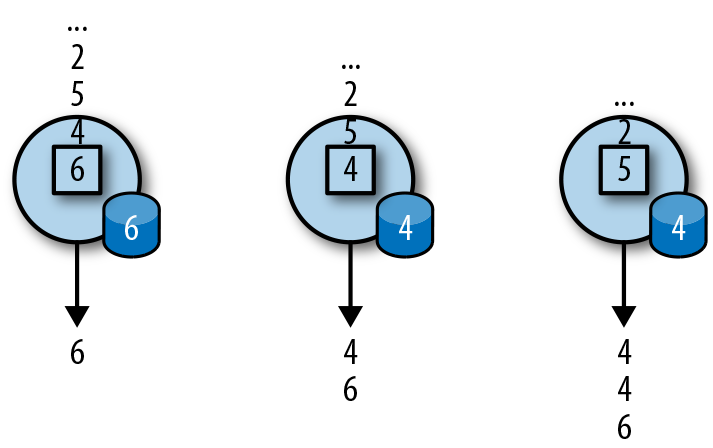
\includegraphics{images/spaf_0205.png}

\hypertarget{ux7a97ux53e3ux64cdux4f5cux7b26}{%
\subsection{窗口操作符}\label{ux7a97ux53e3ux64cdux4f5cux7b26}}

转换和滚动聚合一次处理一个事件产生输出事件并可能更新状态。但是,有些操作必须收集并缓冲数据以计算其结果。
例如,考虑不同流之间的连接或整体聚合这样的操作,例如中值函数。为了在无界流上高效运行这些操作符,我们需要限制
这些操作维护的数据量。在本节中,我们将讨论窗口操作,提供此服务。

窗口还可以在语义上实现关于流的比较复杂的查询。我们已经看到了滚动聚合的方式,以聚合值编码整个流的历史数据来为每个事件提供低延迟的结果。
但如果我们只对最近的数据感兴趣的话会怎样?考虑给司机提供实时交通信息的应用程序。这个程序可以使他们避免拥挤的路线。在这种场景下,你想知道某个位置在最近几分钟内是否有事故发生。
另一方面,了解所有发生过的事故在这个应用场景下并没有什么卵用。更重要的是,通过将流历史缩减为单一聚合值,我们将丢失这段时间内数据的变化。例如,我们可能想知道每5分钟有多少车辆穿过
某个路口。

窗口操作不断从无限事件流中创建有限的事件集,好让我们执行有限集的计算。通常会基于数据属性或基于时间的窗口来分配事件。
要正确定义窗口运算符语义,我们需要确定如何给窗口分配事件以及对窗口中的元素进行求值的频率是什么样的。
窗口的行为由一组策略定义。窗口策略决定何时创建新的窗口以及要分配的事件属于哪个窗口,以及何时对窗口中的元素进行求值。
而窗口的求值基于触发条件。一旦触发条件得到满足,窗口的内容将会被发送到求值函数,求值函数会将计算逻辑应用于窗口中的元素。
求值函数可以是sum或minimal或自定义的聚合函数。
求值策略可以根据时间或者数据属性计算(例如,在过去五秒内收到的事件或者最近的一百个事件等等)。
接下来,我们描述常见窗口类型的语义。

\begin{itemize}
\tightlist
\item
  滚动窗口是将事件分配到固定大小的不重叠的窗口中。当通过窗口的结尾时,全部事件被发送到求值函数进行处理。基于计数的滚动窗口定义了在触发求值之前需要收集多少事件。图2-6显示了一个基于计数的翻滚窗口,每四个元素一个窗口。基于时间的滚动窗口定义一个时间间隔,包含在此时间间隔内的事件。图2-7显示了基于时间的滚动窗口,将事件收集到窗口中每10分钟触发一次计算。
\end{itemize}

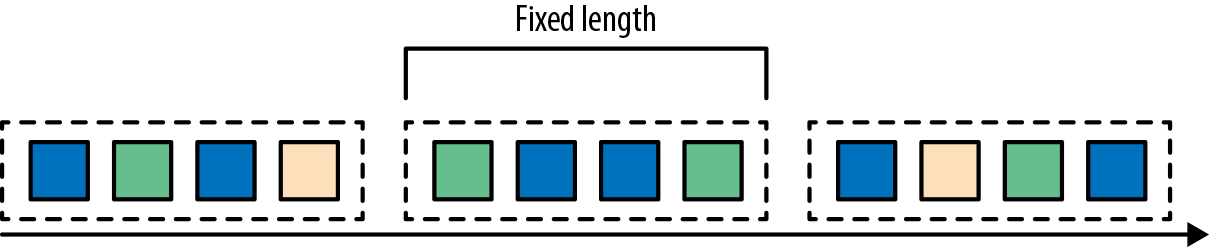
\includegraphics{images/spaf_0206.png}

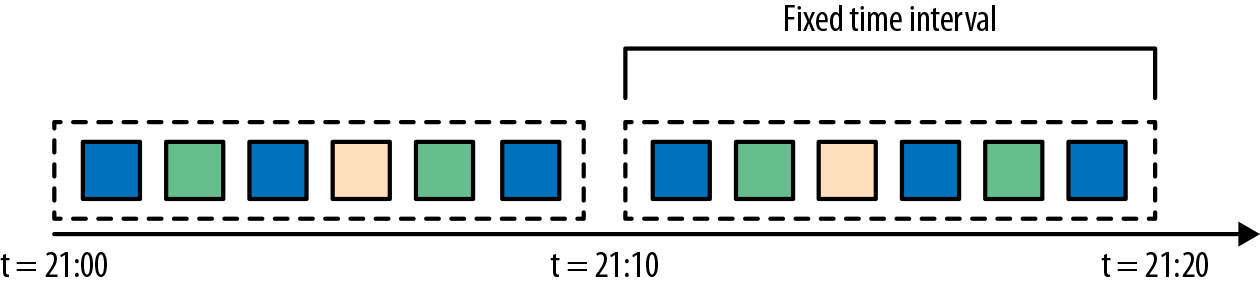
\includegraphics{images/spaf_0207.png}

\begin{itemize}
\tightlist
\item
  滑动窗口将事件分配到固定大小的重叠的窗口中去。因此,事件可能属于多个桶。我们通过提供窗口的长度和滑动距离来定义滑动窗口。滑动距离定义了创建新窗口的间隔。基于滑动计数的窗口,图2-8的长度为四个事件,三个为滑动距离。
\end{itemize}

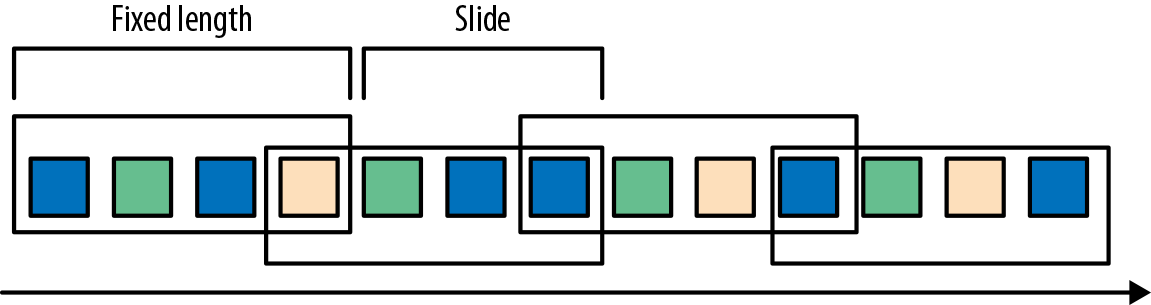
\includegraphics{images/spaf_0208.png}

\begin{itemize}
\tightlist
\item
  会话窗口在常见的真实场景中很有用,一些场景既不能使用滚动窗口也不能使用滑动窗口。考虑一个分析在线用户行为的应用程序。在应用程序里,我们想把源自同一时期的用户活动或会话事件分组在一起。会话由一系列相邻时间发生的事件组成,接下来有一段时间没有活动。例如,用户在App上浏览一系列的新闻,然后关掉App,那么浏览新闻这段时间的浏览事件就是一个会话。会话窗口事先没有定义窗口的长度,而是取决于数据的实际情况,滚动窗口和滑动窗口无法应用于这个场景。相反,我们需要将同一会话中的事件分配到同一个窗口中去,而不同的会话可能窗口长度不一样。会话窗口会定义一个间隙值来区分不同的会话。间隙值的意思是:用户一段时间内不活动,就认为用户的会话结束了。图2-9显示了一个会话窗口。
\end{itemize}

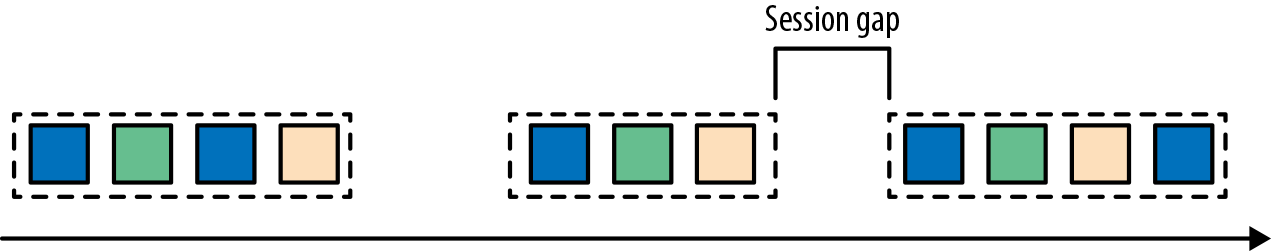
\includegraphics{images/spaf_0209.png}

到目前为止,所有窗口类型都是在整条流上去做窗口操作。但实际上你可能想要将一条流分流成多个逻辑流并定义并行窗口。
例如,如果我们正在接收来自不同传感器的测量结果,那么可能想要在做窗口计算之前按传感器ID对流进行分流操作。
在并行窗口中,每条流都独立于其他流,然后应用了窗口逻辑。图2-10显示了一个基于计数的长度为2的并行滚动窗口,根据事件颜色分流。

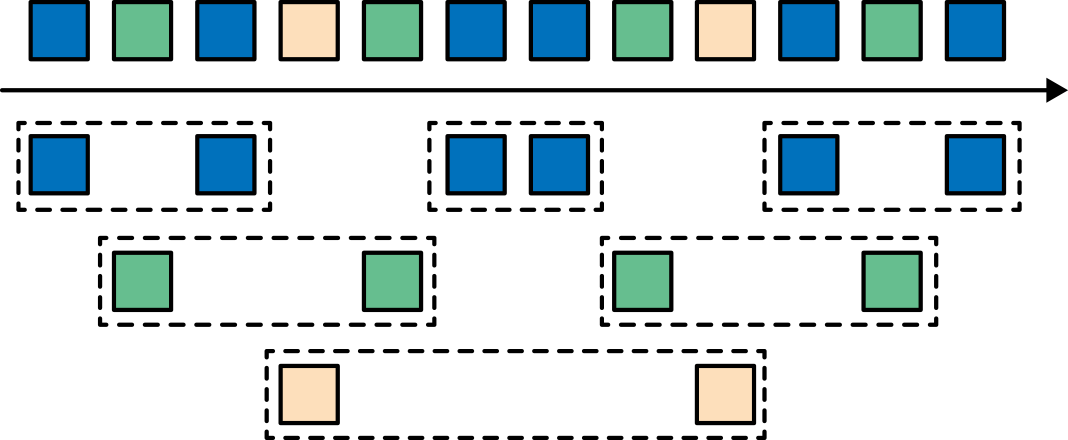
\includegraphics{images/spaf_0210.png}

在流处理中,窗口操作与两个主要概念密切相关:时间语义和状态管理。时间也许是流处理最重要的方面。即使低延迟是流处理的一个有吸引力的特性,它的真正价值不仅仅是快速分析。真实世界的系统,网络和通信渠道远非完美,流数据经常被推迟或无序(乱序)到达。理解如何在这种条件下提供准确和确定的结果是至关重要的。
更重要的是,流处理程序可以按原样处理事件制作的也应该能够处理相同的历史事件方式,从而实现离线分析甚至时间旅行分析。
当然,前提是我们的系统可以保存状态,因为可能有故障发生。到目前为止,我们看到的所有窗口类型在产生结果前都需要保存之前的数据。实际上,如果我们想计算任何指标,即使是简单的计数,我们也需要保存状态。考虑到流处理程序可能会运行几天,几个月甚至几年,我们需要确保状态可以在发生故障的情况下可靠地恢复。
并且即使程序崩溃,我们的系统也能保证计算出准确的结果。本章,我们将在流处理应用可能发生故障的语境下,深入探讨时间和状态的概念。

\hypertarget{ux65f6ux95f4ux8bedux4e49}{%
\section{时间语义}\label{ux65f6ux95f4ux8bedux4e49}}

在本节中,我们将介绍时间语义,并描述流中不同的时间概念。我们将讨论流处理器在乱序事件流的情况下如何提供准确的计算结果,以及我们如何处理历史事件流,如何在流中进行时间旅行。

\hypertarget{ux5728ux6d41ux5904ux7406ux4e2dux4e00ux5206ux949fux4ee3ux8868ux4ec0ux4e48}{%
\subsection{在流处理中一分钟代表什么?}\label{ux5728ux6d41ux5904ux7406ux4e2dux4e00ux5206ux949fux4ee3ux8868ux4ec0ux4e48}}

在处理可能是无限的事件流(包含了连续到达的事件),时间成为流处理程序的核心方面。假设我们想要连续的计算结果,可能每分钟就要计算一次。在我们的流处理程序上下文中,一分钟的意思是什么?

考虑一个程序需要分析一款移动端的在线游戏的用户所产生的事件流。游戏中的用户分了组,而应用程序将收集每个小组的活动数据,基于小组中的成员多快达到了游戏设定的目标,然后在游戏中提供奖励。例如额外的生命和用户升级。例如,如果一个小组中的所有用户在一分钟之内都弹出了500个泡泡,他们将升一级。Alice是一个勤奋的玩家,她在每天早晨的通勤时间玩游戏。问题在于Alice住在柏林,并且乘地铁去上班。而柏林的地铁手机信号很差。我们设想一个这样的场景,Alice当她的手机连上网时,开始弹泡泡,然后游戏会将数据发送到我们编写的应用程序中,这时地铁突然进入了隧道,她的手机也断网了。Alice还在玩这个游戏,而产生的事件将会缓存在手机中。当地铁离开隧道,Alice的手机又在线了,而手机中缓存的游戏事件将发送到应用程序。我们的应用程序应该如何处理这些数据?在这个场景中一分钟的意思是什么?这个一分钟应该包含Alice离线的那段时间吗?下图展示了这个问题。

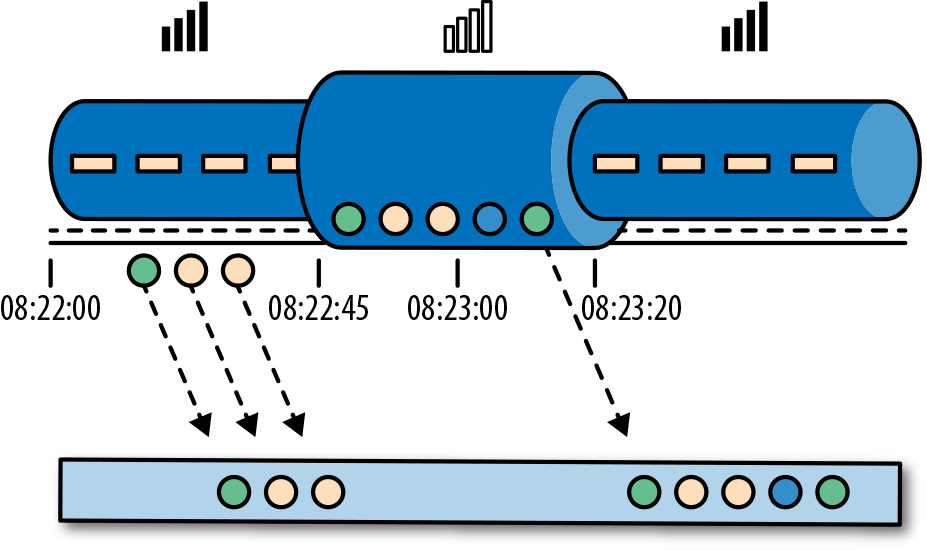
\includegraphics{images/spaf_0211.png}

在线手游是一个简单的场景,展示了应用程序的运算应该取决于事件实际发生的时间,而不是应用程序收到事件的时间。如果我们按照应用程序收到事件的时间来进行处理的话,最糟糕的后果就是,Alice和她的朋友们再也不玩这个游戏了。但是还有很多时间语义非常关键的应用程序,我们需要保证时间语义的正确性。如果我们只考虑我们在一分钟之内收到了多少数据,我们的结果会变化,因为结果取决于网络连接的速度或处理的速度。相反,定义一分钟之内的事件数量,这个一分钟应该是数据本身的时间。

在Alice的这个例子中,流处理程序可能会碰到两个不同的时间概念:处理时间和事件时间。我们将在接下来的部分,讨论这两个概念。

\hypertarget{ux5904ux7406ux65f6ux95f4}{%
\subsection{处理时间}\label{ux5904ux7406ux65f6ux95f4}}

处理时间是处理流的应用程序的机器的本地时钟的时间(墙上时钟)。处理时间的窗口包含了一个时间段内来到机器的所有事件。这个时间段指的是机器的墙上时钟。如下图所示,在Alice的这个例子中,处理时间窗口在Alice的手机离线的情况下,时间将会继续行走。但这个处理时间窗口将不会收集Alice的手机离线时产生的事件。

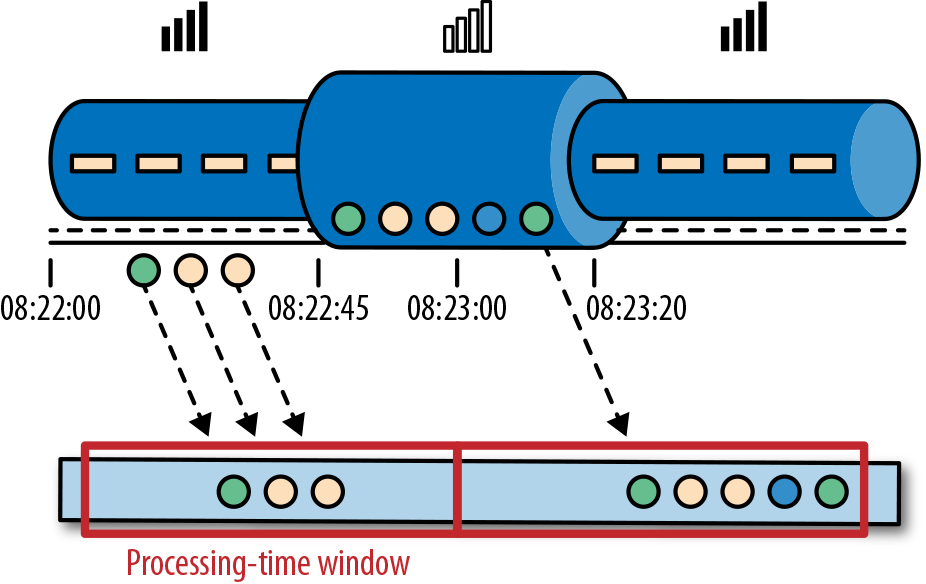
\includegraphics{images/spaf_0212.png}

\hypertarget{ux4e8bux4ef6ux65f6ux95f4}{%
\subsection{事件时间}\label{ux4e8bux4ef6ux65f6ux95f4}}

事件时间是流中的事件实际发生的时间。事件时间基于流中的事件所包含的时间戳。通常情况下,在事件进入流处理程序前,事件数据就已经包含了时间戳。下图展示了事件时间窗口将会正确的将事件分发到窗口中去。可以如实反应事情是怎么发生的。即使事件可能存在延迟。

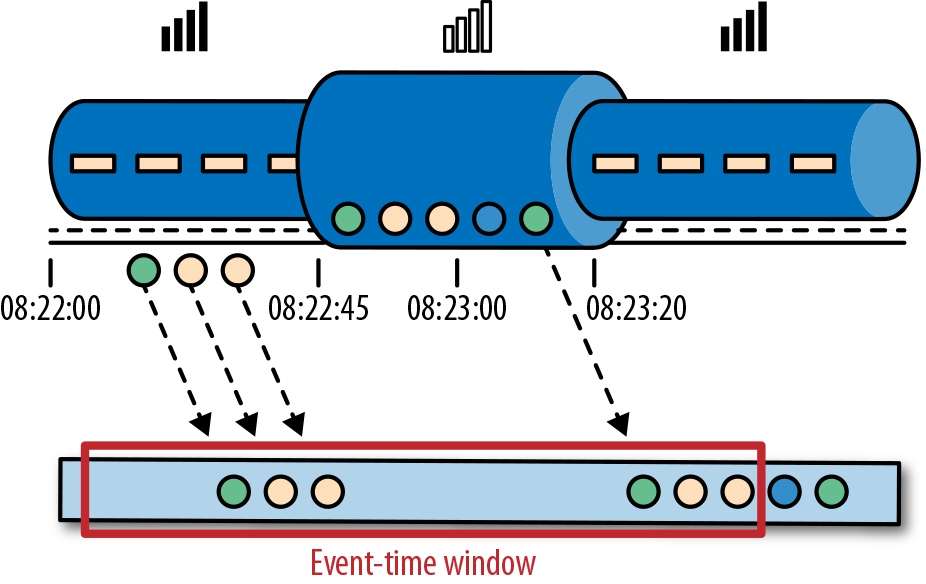
\includegraphics{images/spaf_0213.png}

事件时间使得计算结果的过程不需要依赖处理数据的速度。基于事件时间的操作是可以预测的,而计算结果也是确定的。无论流处理程序处理流数据的速度快或是慢,无论事件到达流处理程序的速度快或是慢,事件时间窗口的计算结果都是一样的。

可以处理迟到的事件只是我们使用事件时间所克服的一个挑战而已。普遍存在的事件乱序问题可以使用事件时间得到解决。考虑和Alice玩同样游戏的Bob,他恰好和Alice在同一趟地铁上。Alice和Bob虽然玩的游戏一样,但他们的手机信号是不同的运营商提供的。当Alice的手机没信号时,Bob的手机依然有信号,游戏数据可以正常发送出去。

如果使用事件时间,即使碰到了事件乱序到达的情况,我们也可以保证结果的正确性。还有,当我们在处理可以重播的流数据时,由于时间戳的确定性,我们可以快进过去。也就是说,我们可以重播一条流,然后分析历史数据,就好像流中的事件是实时发生一样。另外,我们可以快进历史数据来使我们的应用程序追上现在的事件,然后应用程序仍然是一个实时处理程序,而且业务逻辑不需要改变。

\hypertarget{ux6c34ux4f4dux7ebf}{%
\subsection{水位线}\label{ux6c34ux4f4dux7ebf}}

在我们对事件时间窗口的讨论中,我们忽略了一个很重要的方面:我们应该怎样去决定何时触发事件时间窗口的计算?也就是说,在我们可以确定一个时间点之前的所有事件都已经到达之前,我们需要等待多久?我们如何知道事件是迟到的?在分布式系统无法准确预测行为的现实条件下,以及外部组件所引发的事件的延迟,以上问题并没有准确的答案。在本小节中,我们将会看到如何使用水位线来设置事件时间窗口的行为。

水位线是全局进度的度量标准。系统可以确信在一个时间点之后,不会有早于这个时间点发生的事件到来了。本质上,水位线提供了一个逻辑时钟,这个逻辑时钟告诉系统当前的事件时间。当一个运算符接收到含有时间T的水位线时,这个运算符会认为早于时间T的发生的事件已经全部都到达了。对于事件时间窗口和乱序事件的处理,水位线非常重要。运算符一旦接收到水位线,运算符会认为一段时间内发生的所有事件都已经观察到,可以触发针对这段时间内所有事件的计算了。

水位线提供了一种结果可信度和延时之间的妥协。激进的水位线设置可以保证低延迟,但结果的准确性不够。在这种情况下,迟到的事件有可能晚于水位线到达,我们需要编写一些代码来处理迟到事件。另一方面,如果水位线设置的过于宽松,计算的结果准确性会很高,但可能会增加流处理程序不必要的延时。

在很多真实世界的场景里面,系统无法获得足够的知识来完美的确定水位线。在手游这个场景中,我们无法得知一个用户离线时间会有多长,他们可能正在穿越一条隧道,可能正在乘飞机,可能永远不会再玩儿了。水位线无论是用户自定义的或者是自动生成的,在一个分布式系统中追踪全局的时间进度都不是很容易。所以仅仅依靠水位线可能并不是一个很好的主意。流处理系统还需要提供一些机制来处理迟到的元素(在水位线之后到达的事件)。根据应用场景,我们可能需要把迟到事件丢弃掉,或者写到日志里,或者使用迟到事件来更新之前已经计算好的结果。

\hypertarget{ux5904ux7406ux65f6ux95f4ux548cux4e8bux4ef6ux65f6ux95f4}{%
\subsection{处理时间和事件时间}\label{ux5904ux7406ux65f6ux95f4ux548cux4e8bux4ef6ux65f6ux95f4}}

大家可能会有疑问,既然事件时间已经可以解决我们的所有问题,为什么我们还要对比这两个时间概念?真相是,处理时间在很多情况下依然很有用。处理时间窗口将会带来理论上最低的延迟。因为我们不需要考虑迟到事件以及乱序事件,所以一个窗口只需要简单的缓存窗口内的数据即可,一旦机器时间超过指定的处理时间窗口的结束时间,就会触发窗口的计算。所以对于一些处理速度比结果准确性更重要的流处理程序,处理时间就派上用场了。另一个应用场景是,当我们需要在真实的时间场景下,周期性的报告结果时,同时不考虑结果的准确性。一个例子就是一个实时监控的仪表盘,负责显示当事件到达时立即聚合的结果。最后,处理时间窗口可以提供流本身数据的忠实表达,对于一些案例可能是很必要的特性。例如我们可能对观察流和对每分钟事件的计数(检测可能存在的停电状况)很感兴趣。简单的说,处理时间提供了低延迟,同时结果也取决于处理速度,并且也不能保证确定性。另一方面,事件时间保证了结果的确定性,同时还可以使我们能够处理迟到的或者乱序的事件流。

\hypertarget{ux72b6ux6001ux548cux6301ux4e45ux5316ux6a21ux578b}{%
\section{状态和持久化模型}\label{ux72b6ux6001ux548cux6301ux4e45ux5316ux6a21ux578b}}

我们现在转向另一个对于流处理程序非常重要的话题:状态。在数据处理中,状态是普遍存在的。任何稍微复杂一点的计算,都涉及到状态。为了产生计算结果,一个函数在一段时间内的一定数量的事件上来累加状态(例如,聚合计算或者模式匹配)。有状态的运算符使用输入的事件以及内部保存的状态来计算得到输出。例如,一个滚动聚合运算符需要输出这个运算符所观察到的所有事件的累加和。这个运算符将会在内部保存当前观察到的所有事件的累加和,同时每输入一个事件就更新一次累加和的计算结果。相似的,当一个运算符检测到一个``高温''事件紧接着十分钟以内检测到一个``烟雾''事件时,将会报警。直到运算符观察到一个``烟雾''事件或者十分钟的时间段已经过去,这个运算符需要在内部状态中一直保存着``高温''事件。

当我们考虑一下使用批处理系统来分析一个无界数据集时,会发现状态的重要性显而易见。在现代流处理器兴起之前,处理无界数据集的一个通常做法是将输入的事件攒成微批,然后交由批处理器来处理。当一个任务结束时,计算结果将被持久化,而所有的运算符状态就丢失了。一旦一个任务在计算下一个微批次的数据时,这个任务是无法访问上一个任务的状态的(都丢掉了)。这个问题通常使用将状态代理到外部系统(例如数据库)的方法来解决。相反,在一个连续不间断运行的流处理任务中,事件的状态是一直存在的,我们可以将状态暴露出来作为编程模型中的一等公民。当然,我们的确可以使用外部系统来管理流的状态,即使这个解决方案会带来额外的延迟。

由于流处理运算符默认处理的是无界数据流。所以我们必须要注意不要让内部状态无限的增长。为了限制状态的大小,运算符通常情况下会保存一些之前所观察到的事件流的总结或者概要。这个总结可能是一个计数值,一个累加和,或者事件流的采样,窗口的缓存操作,或者是一个自定义的数据结构,这个数据结构用来保存数据流中感兴趣的一些特性。

我们可以想象的到,支持有状态的运算符可能会碰到一些实现上的挑战:

\begin{itemize}
\tightlist
\item
  状态管理:系统需要高效的管理状态,并保证针对状态的并发更新,不会产生竞争条件(race
  condition)。
\item
  状态分区:并行会带来复杂性。因为计算结果同时取决于已经保存的状态和输入的事件流。幸运的是,大多数情况下,我们可以使用Key来对状态进行分区,然后独立的管理每一个分区。例如,当我们处理一组传感器的测量事件流时,我们可以使用分区的运算符状态来针对不同的传感器独立的保存状态。
\item
  状态恢复:第三个挑战是有状态的运算符如何保证状态可以恢复,即使出现任务失败的情况,计算也是正确的。
\end{itemize}

下一节,我们将讨论任务失败和计算结果的保证。

\hypertarget{ux4efbux52a1ux5931ux8d25}{%
\subsection{任务失败}\label{ux4efbux52a1ux5931ux8d25}}

流任务中的运算符状态是很宝贵的,也需要抵御任务失败带来的问题。如果在任务失败的情况下,状态丢失的话,在任务恢复以后计算的结果将是不正确的。流任务会连续不断的运行很长时间,而状态可能已经收集了几天甚至几个月。在失败的情况下,重新处理所有的输入并重新生成一个丢失的状态,将会很浪费时间,开销也很大。

在本章开始时,我们看到如何将流的编程建模成数据流模型。在执行之前,流程序将会被翻译成物理层数据流图,物理层数据流图由连接的并行任务组成,而一个并行任务运行一些运算符逻辑,消费输入流数据,并为其他任务产生输出流数据。真实场景下,可能有数百个这样的任务并行运行在很多的物理机器上。在长时间的运行中,流任务中的任意一个任务在任意时间点都有可能失败。我们如何保证任务的失败能被正确的处理,以使任务能继续的运行下去呢?事实上,我们可能希望我们的流处理器不仅能在任务失败的情况下继续处理数据,还能保证计算结果的正确性以及运算符状态的安全。我们在本小节来讨论这些问题。

\textbf{什么是任务失败?}

对于流中的每一个事件,一个处理任务分为以下步骤:(1)接收事件,并将事件存储在本地的缓存中;(2)可能会更新内部状态;(3)产生输出记录。这些步骤都能失败,而系统必须对于在失败的场景下如何处理有清晰的定义。如果任务在第一步就失败了,事件会丢失吗?如果当更新内部状态的时候任务失败,那么内部状态会在任务恢复以后更新吗?在以上这些场景中,输出是确定性的吗?

在批处理场景下,所有的问题都不是问题。因为我们可以很方便的重新计算。所以不会有事件丢失,状态也可以得到完全恢复。在流的世界里,处理失败不是一个小问题。流系统在失败的情况下需要保证结果的准确性。接下来,我们需要看一下现代流处理系统所提供的一些保障,以及实现这些保障的机制。

\textbf{结果的保证}

当我们讨论保证计算的结果时,我们的意思是流处理器的内部状态需要保证一致性。也就是说我们关心的是应用程序的代码在故障恢复以后看到的状态值是什么。要注意保证应用程序状态的一致性并不是保证应用程序的输出结果的一致性。一旦输出结果被持久化,结果的准确性就很难保证了。除非持久化系统支持事务。

\emph{AT-MOST-ONCE}

当任务故障时,最简单的做法是什么都不干,既不恢复丢失的状态,也不重播丢失的事件。At-most-once语义的含义是最多处理一次事件。换句话说,事件可以被丢弃掉,也没有任何操作来保证结果的准确性。这种类型的保证也叫``没有保证'',因为一个丢弃掉所有事件的系统其实也提供了这样的保障。没有保障听起来是一个糟糕的主意,但如果我们能接受近似的结果,并且希望尽可能低的延迟,那么这样也挺好。

\emph{AT-LEAST-ONCE}

在大多数的真实应用场景,我们希望不丢失事件。这种类型的保障成为at-least-once,意思是所有的事件都得到了处理,而且一些事件还可能被处理多次。如果结果的正确性仅仅依赖于数据的完整性,那么重复处理是可以接受的。例如,判断一个事件是否在流中出现过,at-least-once这样的保证完全可以正确的实现。在最坏的情况下,我们多次遇到了这个事件。而如果我们要对一个特定的事件进行计数,计算结果就可能是错误的了。

为了保证在at-least-once语义的保证下,计算结果也能正确。我们还需要另一套系统来从数据源或者缓存中重新播放数据。持久化的事件日志系统将会把所有的事件写入到持久化存储中。所以如果任务发生故障,这些数据可以重新播放。还有一种方法可以获得同等的效果,就是使用结果承认机制。这种方法将会把每一条数据都保存在缓存中,直到数据的处理等到所有的任务的承认。一旦得到所有任务的承认,数据将被丢弃。

\emph{EXACTLY-ONCE}

恰好处理一次是最严格的保证,也是最难实现的。恰好处理一次语义不仅仅意味着没有事件丢失,还意味着针对每一个数据,内部状态仅仅更新一次。本质上,恰好处理一次语义意味着我们的应用程序可以提供准确的结果,就好像从未发生过故障。

提供恰好处理一次语义的保证必须有至少处理一次语义的保证才行,同时还需要数据重放机制。另外,流处理器还需要保证内部状态的一致性。也就是说,在故障恢复以后,流处理器应该知道一个事件有没有在状态中更新。事务更新是达到这个目标的一种方法,但可能引入很大的性能问题。Flink使用了一种轻量级快照机制来保证恰好处理一次语义。

\emph{端到端恰好处理一次}

目前我们看到的一致性保证都是由流处理器实现的,也就是说都是在Flink流处理器内部保证的。而在真实世界中,流处理应用除了流处理器以外还包含了数据源(例如Kafka)和持久化系统。端到端的一致性保证意味着结果的正确性贯穿了整个流处理应用的始终。每一个组件都保证了它自己的一致性。而整个端到端的一致性级别取决于所有组件中一致性最弱的组件。要注意的是,我们可以通过弱一致性来实现更强的一致性语义。例如,当任务的操作具有幂等性时,比如流的最大值或者最小值的计算。在这种场景下,我们可以通过最少处理一次这样的一致性来实现恰好处理一次这样的最高级别的一致性。

\hypertarget{flinkux8fd0ux884cux67b6ux6784}{%
\chapter{Flink运行架构}\label{flinkux8fd0ux884cux67b6ux6784}}

\hypertarget{ux7cfbux7edfux67b6ux6784}{%
\section{系统架构}\label{ux7cfbux7edfux67b6ux6784}}

Flink是一个用于有状态的并行数据流处理的分布式系统。它由多个进程构成,这些进程一般会分布运行在不同的机器上。对于分布式系统来说,面对的常见问题有:集群中资源的分配和管理、进程协调调度、持久化和高可用的数据存储,以及故障恢复。

对于这些分布式系统的经典问题,业内已有比较成熟的解决方案和服务。所以Flink并不会自己去处理所有的问题,而是利用了现有的集群架构和服务,这样它就可以把精力集中在核心工作------分布式数据流处理上了。Flink与一些集群资源管理工具有很好的集成,比如Apache
Mesos、YARN和Kubernetes;同时,也可以配置为独立(stand-alone)集群运行。Flink自己并不提供持久化的分布式存储,而是直接利用了已有的分布式文件系统(比如HDFS)或者对象存储(比如S3)。对于高可用的配置,Flink需要依靠Apache
ZooKeeper来完成。

在本节中,我们将介绍Flink的不同组件,以及在运行程序时它们如何相互作用。我们会讨论部署Flink应用程序的两种模式,并且了解每种模式下分发和执行任务的方式。最后,我们还会解释一下Flink的高可用性模式是如何工作的。

\hypertarget{flinkux8fd0ux884cux65f6ux7ec4ux4ef6}{%
\subsection{Flink运行时组件}\label{flinkux8fd0ux884cux65f6ux7ec4ux4ef6}}

Flink运行时架构主要包括四个不同的组件,它们会在运行流处理应用程序时协同工作:作业管理器(JobManager)、资源管理器(ResourceManager)、任务管理器(TaskManager),以及分发器(Dispatcher)。因为Flink是用Java和Scala实现的,所以所有组件都会运行在Java虚拟机(JVMs)上。每个组件的职责如下:

\begin{itemize}
\tightlist
\item
  作业管理器(JobManager)是控制一个应用程序执行的主进程,也就是说,每个应用程序都会被一个不同的作业管理器所控制执行。作业管理器会先接收到要执行的应用程序。这个应用程序会包括:作业图(JobGraph)、逻辑数据流图(logical
  dataflow
  graph)和打包了所有的类、库和其它资源的JAR包。作业管理器会把JobGraph转换成一个物理层面的数据流图,这个图被叫做``执行图''(ExecutionGraph),包含了所有可以并发执行的任务。作业管理器会向资源管理器(ResourceManager)请求执行任务必要的资源,也就是任务管理器(TaskManager)上的插槽(slot)。一旦它获取到了足够的资源,就会将执行图分发到真正运行它们的TaskManager上。而在运行过程中,作业管理器会负责所有需要中央协调的操作,比如说检查点(checkpoints)的协调。
\item
  ResourceManager主要负责管理任务管理器(TaskManager)的插槽(slot),TaskManger插槽是Flink中定义的处理资源单元。Flink为不同的环境和资源管理工具提供了不同资源管理器(ResourceManager),比如YARN、Mesos、K8s,以及standalone部署。当作业管理器申请插槽资源时,ResourceManager会将有空闲插槽的TaskManager分配给作业管理器。如果ResourceManager没有足够的插槽来满足作业管理器的请求,它还可以向资源提供平台发起会话,以提供启动TaskManager进程的容器。另外,ResourceManager还负责终止空闲的TaskManager,释放计算资源。
\item
  任务管理器(TaskManager)是Flink中的工作进程。通常在Flink中会有多个TaskManager运行,每一个TaskManager都包含了一定数量的插槽(slots)。插槽的数量限制了TaskManager能够执行的任务数量。启动之后,TaskManager会向资源管理器注册它的插槽;收到资源管理器的指令后,TaskManager就会将一个或者多个插槽提供给作业管理器调用。作业管理器就可以向插槽分配任务(tasks)来执行了。在执行过程中,一个TaskManager可以跟其它运行同一应用程序的TaskManager交换数据。任务的执行和插槽的概念会在``任务执行''一节做具体讨论。
\item
  分发器(Dispatcher)可以跨作业运行,它为应用提交提供了REST接口。当一个应用被提交执行时,分发器就会启动并将应用移交给一个作业管理器。由于是REST接口,所以Dispatcher可以作为集群的一个HTTP接入点,这样就能够不受防火墙阻挡。Dispatcher也会启动一个Web
  UI,用来方便地展示和监控作业执行的信息。Dispatcher在架构中可能并不是必需的,这取决于应用提交运行的方式。
\end{itemize}

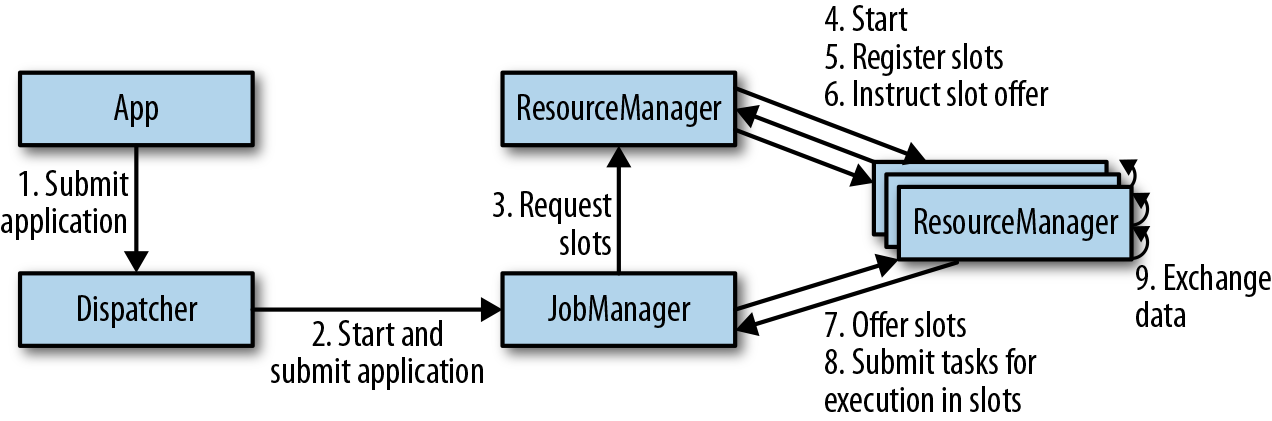
\includegraphics{images/spaf_0301.png}

\begin{quote}
上图是从一个较为高层级的视角,来看应用中各组件的交互协作。如果部署的集群环境不同(例如YARN,Mesos,Kubernetes,standalone等),其中一些步骤可以被省略,或是有些组件会运行在同一个JVM进程中。
\end{quote}

\hypertarget{ux5e94ux7528ux90e8ux7f72}{%
\subsection{应用部署}\label{ux5e94ux7528ux90e8ux7f72}}

Flink应用程序可以用以下两种不同的方式部署:

\emph{框架(Framework)方式}

在这个模式下,Flink应用被打包成一个Jar文件,并由客户端提交给一个运行服务(running
service)。这个服务可以是一个Flink的Dispatcher,也可以是一个Flink的作业管理器,或是Yarn的ResourceManager。如果application被提交给一个作业管理器,则它会立即开始执行这个application。如果application被提交给了一个Dispatcher,或是Yarn
ResourceManager,则它会启动一个作业管理器,然后将application交给它,再由作业管理器开始执行此应用。

\emph{库(Library)方式}

在这个模式下,Flink Application 会被打包在一个容器(container)
镜像里,例如一个Docker
镜像。此镜像包含了运行作业管理器和ResourceManager的代码。当一个容器从镜像启动后,它会自动启动ResourceManager和作业管理器,并提交打包好的应用。另一种方法是:将应用打包到镜像后,只用于部署TaskManager容器。从镜像启动的容器会自动启动一个TaskManager,然后连接ResourceManager并注册它的slots。这些镜像的启动以及失败重启,通常都会由一个外部的资源管理器管理(比如Kubernetes)。

框架模式遵循了传统的任务提交方式,从客户端提交到Flink运行服务。而在库模式下,没有运行的Flink服务。它是将Flink作为一个库,与应用程序一同打包到了一个容器镜像。这种部署方式在微服务架构中较为常见。我们会在``运行管理流式应用程序''一节对这个话题做详细讨论。

\hypertarget{ux4efbux52a1ux6267ux884c}{%
\subsection{任务执行}\label{ux4efbux52a1ux6267ux884c}}

一个TaskManager可以同时执行多个任务(tasks)。这些任务可以是同一个算子(operator)的子任务(数据并行),也可以是来自不同算子的(任务并行),甚至可以是另一个不同应用程序的(作业并行)。TaskManager提供了一定数量的处理插槽(processing
slots),用于控制可以并行执行的任务数。一个slot可以执行应用的一个分片,也就是应用中每一个算子的一个并行任务。图3-2展示了TaskManagers,slots,tasks以及operators之间的关系:

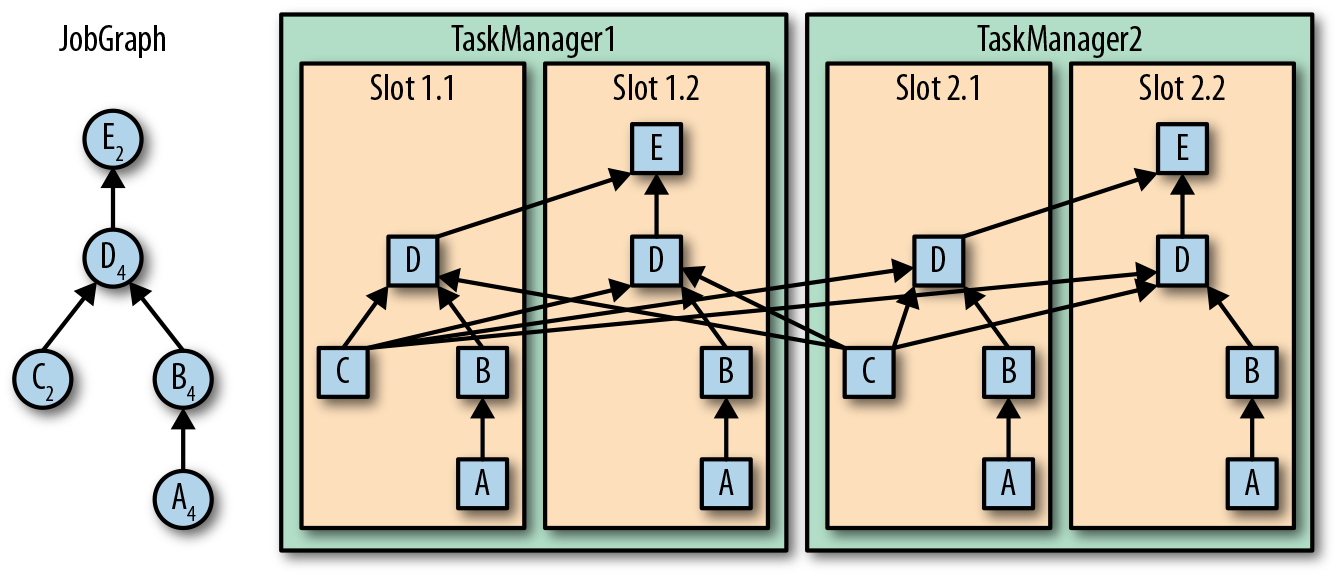
\includegraphics{images/spaf_0302.png}

最左边是一个``作业图''(JobGraph),包含了5个算子------它是应用程序的非并行表示。其中算子A和C是数据源(source),E是输出端(sink)。C和E并行度为2,而其他的算子并行度为4。因为最高的并行度是4,所以应用需要至少四个slot来执行任务。现在有两个TaskManager,每个又各有两个slot,所以我们的需求是满足的。作业管理器将JobGraph转化为``执行图''(ExecutionGraph),并将任务分配到四个可用的slot上。对于有4个并行任务的算子,它的task会分配到每个slot上。而对于并行度为2的operator
C和E,它们的任务被分配到slot 1.1、2.1 以及 slot
1.2、2.2。将tasks调度到slots上,可以让多个tasks跑在同一个TaskManager内,也就可以是的tasks之间的数据交换更高效。然而将太多任务调度到同一个TaskManager上会导致TaskManager过载,继而影响效率。之后我们会在``控制任务调度''一节继续讨论如何控制任务的调度。

TaskManager在同一个JVM中以多线程的方式执行任务。线程较进程会更轻量级,但是线程之间并没有对任务进行严格隔离。所以,单个任务的异常行为有可能会导致整个TaskManager进程挂掉,当然也同时包括运行在此进程上的所有任务。通过为每个TaskManager配置单独的slot,就可以将应用在TaskManager上相互隔离开来。TaskManager内部有多线程并行的机制,而且在一台主机上可以部署多个TaskManager,所以Flink在资源配置上非常灵活,在部署应用时可以充分权衡性能和资源的隔离。我们将会在第九章对Flink集群的配置和搭建继续做详细讨论。

\hypertarget{ux9ad8ux53efux7528ux914dux7f6e}{%
\subsection{高可用配置}\label{ux9ad8ux53efux7528ux914dux7f6e}}

流式应用程序一般被设计为7 x
24小时运行。所以很重要的一点是:即使出现了进程挂掉的情况,应用仍需要继续保持运行。为了从故障恢复,系统首先需要重启进程、然后重启应用并恢复它的状态。接下来,我们就来了解Flink如何重启失败的进程。

\emph{TaskManager故障}

如前所述,Flink需要足够数目的slot,来执行一个应用的所有任务。假设一个Flink环境有4个TaskManager,每个提供2个插槽,那么流应用程序执行的最高并行度为8。如果其中一个TaskManager挂掉了,那么可用的slots会降到6。在这种情况下,作业管理器会请求ResourceManager提供更多的slots。如果此请求无法满足------例如应用跑在一个独立集群------那么作业管理器在有足够的slots之前,无法重启应用。应用的重启策略决定了作业管理器的重启频率,以及两次重启尝试之间的时间间隔。

\emph{作业管理器故障}

比TaskManager故障更严重的问题是作业管理器故障。作业管理器控制整个流应用程序的执行,并维护执行中的元数据------例如指向已完成检查点的指针。若是对应的作业管理器挂掉,则流程序无法继续运行。所以这就导致在Flink应用中,作业管理器是单点故障。为了解决这个问题,Flink提供了高可用模式。在原先的作业管理器挂掉后,可以将一个作业的状态和元数据迁移到另一个作业管理器,并继续执行。

Flink的高可用模式基于Apache
ZooKeeper,我们知道,ZooKeeper是用来管理需要协调和共识的分布式服务的系统。Flink主要利用ZooKeeper来进行领导者(leader)的选举,并把它作为一个高可用和持久化的数据存储。当在高可用模式下运行时,作业管理器会将JobGraph以及所有需要的元数据(例如应用程序的jar文件),写入到一个远程的持久化存储系统中。而且,作业管理器会将指向存储位置的指针,写入到ZooKeeper的数据存储中。在执行一个应用的过程中,作业管理器会接收每个独立任务检查点的状态句柄(也就是存储位置)。当一个检查点完成时(所有任务已经成功地将它们的状态写入到远程存储),
作业管理器把状态句柄写入远程存储,并将指向这个远程存储的指针写入ZooKeeper。这样,一个作业管理器挂掉之后再恢复,所需要的所有数据信息已经都保存在了远程存储,而ZooKeeper里存有指向此存储位置的指针。图3-3描述了这个设计:

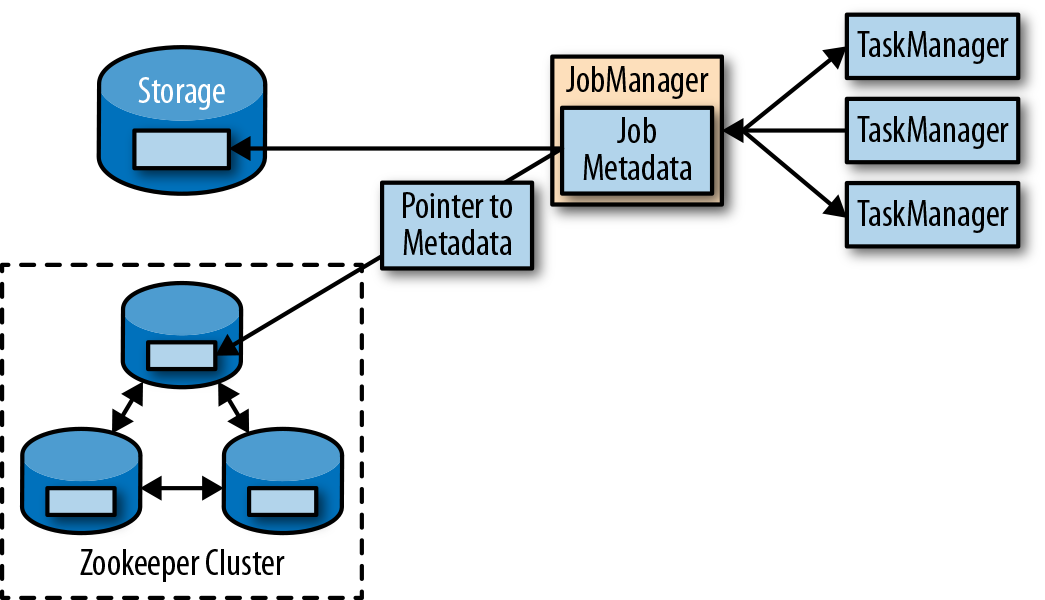
\includegraphics{images/spaf_0303.png}

当一个作业管理器失败,所有属于这个应用的任务都会自动取消。一个新的作业管理器接管工作,会执行以下操作:

\begin{itemize}
\tightlist
\item
  从ZooKeeper请求存储位置(storage
  location),从远端存储获取JobGraph,Jar文件,以及应用最近一次检查点(checkpoint)的状态句柄(state
  handles)
\item
  从ResourceManager请求slots,用来继续运行应用
\item
  重启应用,并将所有任务的状态,重设为最近一次已完成的检查点
\end{itemize}

如果我们是在容器环境里运行应用(如Kubernetes),故障的作业管理器或TaskManager
容器通常会由容器服务自动重启。当运行在YARN或Mesos之上时,作业管理器或TaskManager进程会由Flink的保留进程自动触发重启。而在standalone模式下,Flink并未提供重启故障进程的工具。所以,此模式下我们可以增加备用(standby)的
作业管理器和TaskManager,用于接管故障的进程。我们将会在``高可用配置''一节中做进一步讨论。

\hypertarget{flinkux4e2dux7684ux6570ux636eux4f20ux8f93}{%
\section{Flink中的数据传输}\label{flinkux4e2dux7684ux6570ux636eux4f20ux8f93}}

\hypertarget{ux57faux4e8eux4fe1ux4efbux5ea6ux7684ux6d41ux63a7ux5236}{%
\subsection{基于信任度的流控制}\label{ux57faux4e8eux4fe1ux4efbux5ea6ux7684ux6d41ux63a7ux5236}}

通过网络连接来发送每条数据的效率很低,会导致很大的开销。为了充分利用网络连接的带宽,就需要进行缓冲了。在流处理的上下文中,缓冲的一个缺点是会增加延迟,因为数据需要在缓冲区中进行收集,而不是立即发送。

Flink实现了一个基于信任度的流量控制机制,其工作原理如下。接收任务授予发送任务一些``信任度''(credit),也就是为了接收其数据而保留的网络缓冲区数。当发送者收到一个信任度通知,它就会按照被授予的信任度,发送尽可能多的缓冲数据,并且同时发送目前积压数据的大小------也就是已填满并准备发送的网络缓冲的数量。接收者用保留的缓冲区处理发来的数据,并对发送者传来的积压量进行综合考量,为其所有连接的发送者确定下一个信用度授权的优先级。

基于信用度的流控制可以减少延迟,因为发送者可以在接收者有足够的资源接受数据时立即发送数据。此外,在数据倾斜的情况下,这样分配网络资源是一种很有效的机制,因为信用度是根据发送者积压数据量的规模授予的。因此,基于信用的流量控制是Flink实现高吞吐量和低延迟的重要组成部分。

\hypertarget{ux4efbux52a1ux94fe}{%
\subsection{任务链}\label{ux4efbux52a1ux94fe}}

Flink采用了一种称为任务链的优化技术,可以在特定条件下减少本地通信的开销。为了满足任务链的要求,必须将两个或多个算子设为相同的并行度,并通过本地转发(local
forward)的方式进行连接。图3-5所示的算子管道满足这些要求。它由三个算子组成,这些算子的任务并行度都被设为2,并且通过本地转发方式相连接。

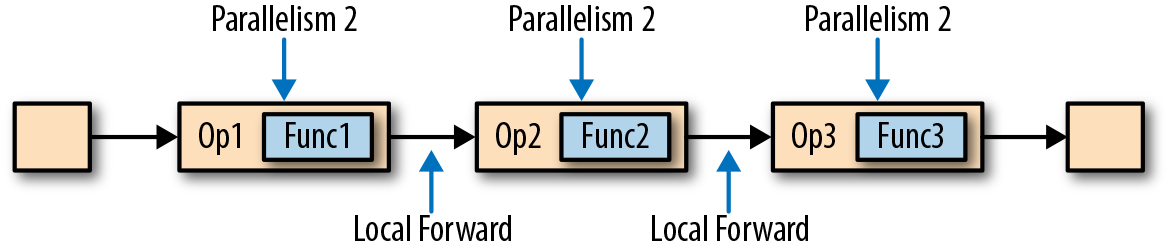
\includegraphics{images/spaf_0305.png}

图3-6展示了管道以任务链方式运行的过程。算子的函数被融合成了一个单一的任务,由一个线程执行。由函数生成的数据通过一个简单的方法调用移交给下一个函数;这样在函数之间直接传递数据,基本上没有序列化和通信成本。

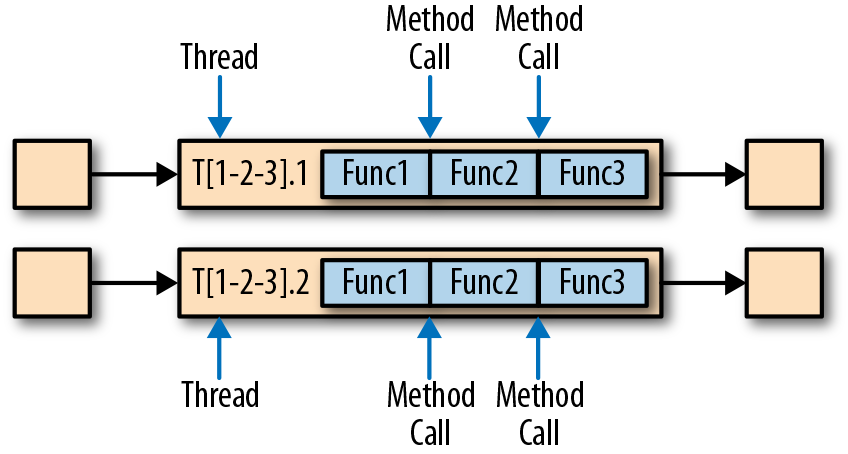
\includegraphics{images/spaf_0306.png}

任务链可以显著降低本地任务之间的通信成本,但也有一些场景,在没有链接的情况下运行管道操作是有意义的。例如,如果任务链中某个函数执行的开销巨大,那就可以将一条长的任务链管道断开,或者将一条链断开为两个任务,从而可以将这个开销大的函数调度到不同的槽(slots)中。图3-7显示了在没有任务链的情况下相同管道操作的执行情况。所有函数都由独立的单个任务来评估,每个任务都在专有的线程中运行。

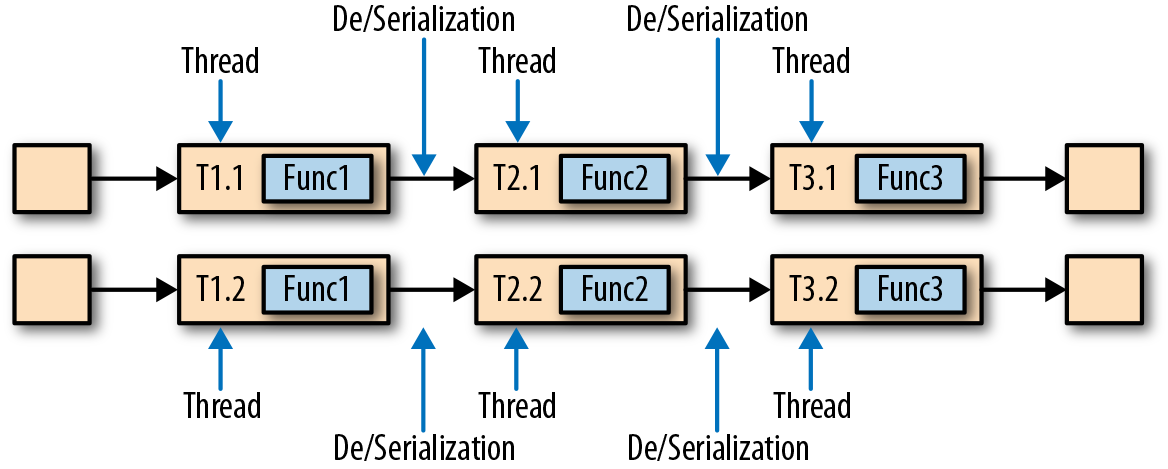
\includegraphics{images/spaf_0307.png}

任务链在Flink中默认会启用。在``控制任务链''一节中,我们展示了如何禁用应用程序的任务链,以及如何控制各个算子的链接行为。

\hypertarget{ux4e8bux4ef6ux65f6ux95f4ux5904ux7406}{%
\section{事件时间处理}\label{ux4e8bux4ef6ux65f6ux95f4ux5904ux7406}}

在``时间语义''一节,我们重点强调了时间语义在流处理应用中的重要性,并且解释了处理时间(processing
time)和事件时间(event
time)的不同。处理时间比较好理解,因为它是基于处理器本地时间的;但同时,它会带来比较混乱、不一致、并且不可重现的结果。相比之下,事件时间语义能够产生可重现且一致的结果,这也是许多流处理场景希望解决的一大难题。但是,与处理时间应用程序相比,事件时间应用程序会更复杂,需要额外的配置。另外,支持事件时间的流处理器,也比纯粹在处理时间中运行的系统内部更为复杂。

Flink为常见的事件时间处理操作提供了直观且易于使用的原语,同时暴露了表达性很强的API,用户可以使用自定义算子实现更高级的事件时间应用程序。很好地理解Flink的内部时间处理,对于实现这样的高级应用程序会有很大帮助,有时也是必需的。上一章介绍了Flink利用两个概念来支持事件时间语义:记录时间戳(timestamps)和水位线(watermarks)。接下来,我们将描述Flink如何在内部实现并处理时间戳和水位线,进而支持具有事件时间语义的流式应用程序。

\hypertarget{ux65f6ux95f4ux6233}{%
\subsection{时间戳}\label{ux65f6ux95f4ux6233}}

由Flink事件时间流应用程序处理的所有记录都必须伴有时间戳。时间戳将数据与特定时间点相关联,通常就是数据所表示的事件发生的时间点。而只要时间戳大致跟数据流保持一致,基本上随着数据流的前进而增大,应用程序就可以自由选择时间戳的含义。不过正如``时间语义''一节中所讨论的,在现实场景中,时间戳基本上都是乱序的,所以采用``事件时间''而非``处理事件''往往会显得更为重要。

当Flink以事件时间模式处理数据流时,它会根据数据记录的时间戳来处理基于时间的算子。例如,时间窗口算子根据相关时间戳将数据分配给不同的时间窗口。Flink将时间戳编码为16字节的长整型值,并将其作为元数据附加到数据记录中。它的内置运算符会将这个长整型值解释为一个具有毫秒精度的Unix时间戳,也就是1970-01-01-00:00:00.000以来的毫秒数。当然,如果用户进行了自定义,那么运算符可以有自己的解释,例如,可以将精度调整到微秒。

\hypertarget{ux6c34ux4f4dux7ebf-1}{%
\subsection{水位线}\label{ux6c34ux4f4dux7ebf-1}}

除了时间戳,基于事件时间的Flink应用程序还必须支持水位线(watermark)。在基于事件时间的应用中,水位线用于生成每个任务的当前事件时间。基于时间的算子使用这个``当前事件时间''来触发计算和处理操作。例如,一个时间窗口任务(time-window
task)会在任务的事件时间超出窗口的关闭边界时,完成窗口计算,并输出计算结果。

在Flink中,水位线被实现为一条特殊的数据记录,它里面以长整型值保存了一个时间戳。水位线在带有时间戳的数据流中,跟随着其它数据一起流动,如图3-8所示。

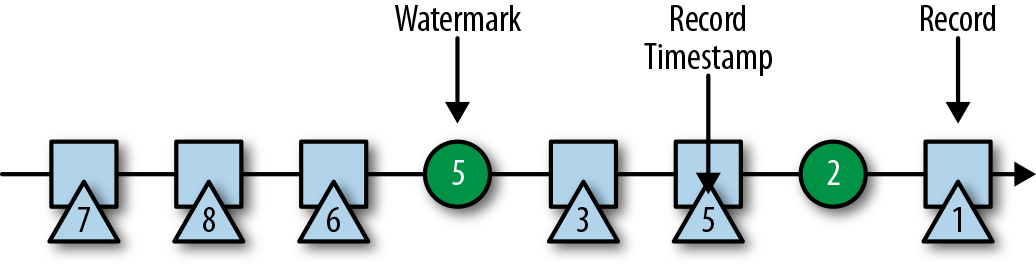
\includegraphics{images/spaf_0308.png}

水位线有两个基本属性:

\begin{itemize}
\tightlist
\item
  必须单调递增,以确保任务的事件时间时钟在向前推进,而不是在后退。
\item
  它们与数据的时间戳相关。带有时间戳T的水位线表示,所有后续数据的时间戳都应该大于T。
\end{itemize}

上面的第二个属性用于处理带有乱序时间戳的数据流,比如图3-8中时间戳3和5的数据。基于时间的算子任务会收集和处理数据(这些数据可能具有乱序的时间戳),并在事件时间时钟到达某个时刻时完成计算。这个时刻就表示数据收集的截止,具有之前时间戳的数据应该都已经到达、不再需要了;而其中的事件时间时钟,正是由当前接收到的水位线来指示的。如果任务再接收到的数据违反了watermark的这一属性,也就是时间戳小于以前接收到的水位线时,它所属的那部分计算可能已经完成了。这种数据被称为延迟数据(late
records)。Flink提供了处理延迟数据的不同方式,我们会在``处理延迟数据''一节中讨论。

水位线还有一个很有趣的特性,它允许应用程序自己来平衡结果的完整性和延迟。如果水位线与数据的时间戳非常接近,那么我们可以得到较低的处理延迟,因为任务在完成计算之前只会短暂地等待更多数据到达。而同时,结果的完整性可能会受到影响,因为相关数据可能因为迟到而被视为``延迟数据'',这样就不会包含在结果中。相反,非常保守的水位线提供了足够的时间去等待所有数据到达,这样会增加处理延迟,但提高了结果的完整性。

\hypertarget{watermarkux7684ux4f20ux9012ux548cux4e8bux4ef6ux65f6ux95f4}{%
\subsection{watermark的传递和事件时间}\label{watermarkux7684ux4f20ux9012ux548cux4e8bux4ef6ux65f6ux95f4}}

在本节中,我们将讨论算子如何处理水位线。Flink把watermark作为一条特殊的数据来实现,它也会由算子任务接收和发送。任务会有一个内部的时间服务,它会维护定时器,并在收到watermark时触发。任务可以在计时器服务中注册定时器,以便在将来特定的时间点执行计算。例如,窗口算子为每个活动窗口注册一个定时器,当事件时间超过窗口的结束时间时,该计时器将清除窗口的状态。

当任务收到watermark时,将执行以下操作:

\begin{itemize}
\tightlist
\item
  任务根据watermark的时间戳更新其内部事件时钟。
\item
  任务的时间服务会将所有过期的计时器标识出来,它们的时间小于当前的事件时间。对于每个过期的计时器,任务调用一个回调函数,该函数可以执行计算并发送结果。
\item
  任务会发出一个带有更新后的事件时间的watermark。
\end{itemize}

\begin{quote}
Flink限制通过DataStream
API访问时间戳和watermark。函数不能读取或修改数据的时间戳和watermark,但底层的``处理函数''(process
functions)除外,它们可以读取当前处理数据的时间戳、请求算子的当前事件时间,还可以注册定时器。通常的函数都不会暴露这些可以设置时间戳、操作任务事件时间时钟、或者发出水位线的API。而基于时间的数据流算子任务则会配置发送出的数据的时间戳,以确保它们能够与已到达的水位线平齐。例如,窗口计算完成后,时间窗口的算子任务会将窗口的结束时间作为时间戳附加到将要发送出的结果数据上,然后再使用触发窗口计算的时间戳发出watermark。
\end{quote}

现在,让我们更详细地解释一下任务在接收到新的watermark时,如何继续发送watermark并更新其事件时钟。正如我们在``数据并发和任务并发''中所了解的,Flink将数据流拆分为多个分区,并通过单独的算子任务并行地处理每个分区。每个分区都是一个流,里面包含了带着时间戳的数据和watermark。一个算子与它前置或后续算子的连接方式有多种情况,所以它对应的任务可以从一个或多个``输入分区''接收数据和watermark,同时也可以将数据和watermark发送到一个或多个``输出分区''。接下来,我们将详细描述一个任务如何向多个输出任务发送watermark,以及如何通过接收到的watermark来驱动事件时间时钟前进。

任务为每个输入分区维护一个分区水位线(watermark)。当从一个分区接收到watermark时,它会比较新接收到的值和当前水位值,然后将相应的分区watermark更新为两者的最大值。然后,任务会比较所有分区watermark的大小,将其事件时钟更新为所有分区watermark的最小值。如果事件时间时钟前进了,任务就将处理所有被触发的定时器操作,并向所有连接的输出分区发送出相应的watermark,最终将新的事件时间广播给所有下游任务。

图3-9显示了具有四个输入分区和三个输出分区的任务如何接收watermark、更新分区watermark和事件时间时钟,以及向下游发出watermark。

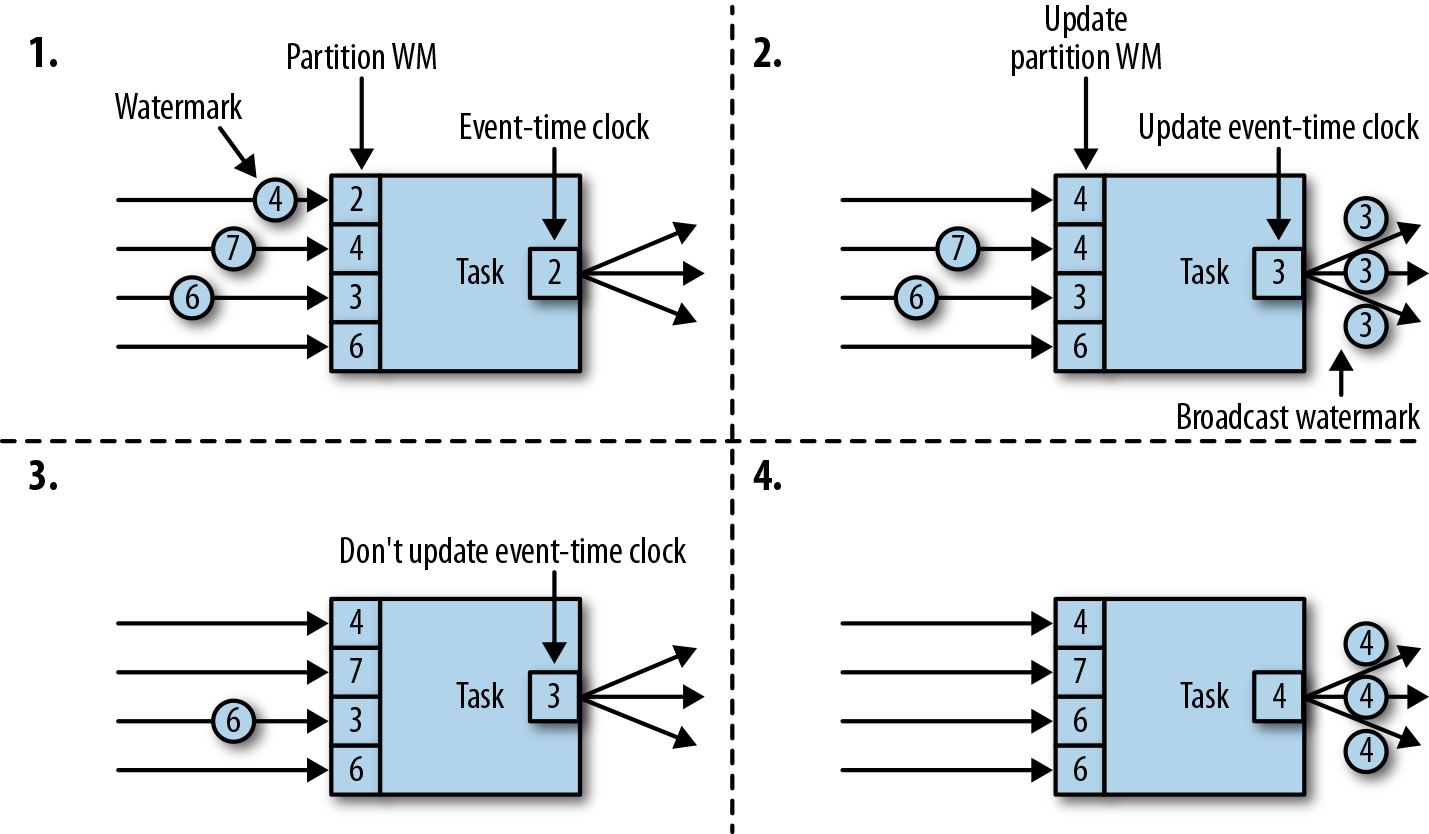
\includegraphics{images/spaf_0309.png}

具有两个或多个输入流(如Union或CoFlatMap)的算子任务(参见``多流转换''一节)也会以所有分区watermark的最小值作为事件时间时钟。它们并不区分不同输入流的分区watermark,所以两个输入流的数据都是基于相同的事件时间时钟进行处理的。当然我们可以想到,如果应用程序的各个输入流的事件时间不一致,那么这种处理方式可能会导致问题。

Flink的水位处理和传递算法,确保了算子任务发出的时间戳和watermark是``对齐''的。不过它依赖一个条件,那就是所有分区都会提供不断增长的watermark。一旦一个分区不再推进水位线的上升,或者完全处于空闲状态、不再发送任何数据和watermark,任务的事件时间时钟就将停滞不前,任务的定时器也就无法触发了。对于基于时间的算子来说,它们需要依赖时钟的推进来执行计算和清除状态,这种情况显然就会有问题。如果任务没有定期从所有输入任务接收到新的watermark,那么基于时间的算子的处理延迟和状态空间的大小都会显著增加。

对于具有两个输入流而且watermark明显不同的算子,也会出现类似的情况。具有两个输入流的任务的事件时间时钟,将会同较慢的那条流的watermark保持一致,而通常较快流的数据或者中间结果会在state中缓冲,直到事件时间时钟达到这条流的watermark,才会允许处理它们。

\hypertarget{ux65f6ux95f4ux6233ux7684ux5206ux914dux548cux6c34ux4f4dux7ebfux7684ux4ea7ux751f}{%
\subsection{时间戳的分配和水位线的产生}\label{ux65f6ux95f4ux6233ux7684ux5206ux914dux548cux6c34ux4f4dux7ebfux7684ux4ea7ux751f}}

我们已经解释了什么是时间戳和水位线,以及它们是如何由Flink内部处理的;然而我们还没有讨论它们的产生。流应用程序接收到数据流时,通常就会先分配时间戳并生成水位线(watermark)。因为时间戳的选择是由不同的应用程序决定的,而且watermark取决于时间戳和流的特性,所以应用程序必须首先显式地分配时间戳并生成watermark。Flink流应用程序可以通过三种方式分配时间戳和生成watermark:

\begin{itemize}
\tightlist
\item
  在数据源(source)处分配:当数据流被摄入到应用程序中时,可以由``源函数''SourceFunction分配和生成时间戳和watermark。SourceFunction可以产生并发送一个数据流;数据会与相关的时间戳一起发送出去,而watermark可以作为一条特殊数据在任何时间点发出。如果SourceFunction(暂时)不再发出watermark,它可以声明自己处于``空闲''(idle)状态。Flink会在后续算子的水位计算中,把空闲的SourceFunction产生的流分区排除掉。source的这一空闲机制,可以用来解决前面提到的水位不再上升的问题。源函数(Source
  Function)在``实现自定义源函数''一节中进行了更详细的讨论。
\item
  定期分配:在Flink中,DataStream
  API提供一个名为AssignerWithPeriodicWatermarks的用户定义函数,它可以从每个数据中提取时间戳,并被定期调用以生成当前watermark。提取出的时间戳被分配给相应的数据,而生成的watermark也会添加到流中。这个函数将在``分配时间戳和生成水位线''一节中讨论。
\item
  间断分配:AssignerWithPunctuatedWatermarks是另一个用户定义的函数,它同样会从每个数据中提取一个时间戳。它可以用于生成特殊输入数据中的watermark。与AssignerWithPeriodicWatermarks相比,此函数可以(但不是必须)从每个记录中提取watermark。我们在``分配时间戳和生成水位线''一节中同样讨论了该函数。
\end{itemize}

用户定义的时间戳分配函数并没有严格的限制,通常会放在尽可能靠近source算子的位置,因为当经过一些算子处理后,数据及其时间戳的顺序就更加难以解释了。所以尽管我们可以在流应用程序的中段覆盖已有的时间戳和watermark------Flink通过用户定义的函数提供了这种灵活性,但这显然并不是推荐的做法。

\hypertarget{ux72b6ux6001ux7ba1ux7406}{%
\section{状态管理}\label{ux72b6ux6001ux7ba1ux7406}}

在第2章中,我们已经知道大多数流应用程序都是有状态的。许多算子会不断地读取和更新状态,例如在窗口中收集的数据、读取输入源的位置,或者像机器学习模型那样的用户定制化的算子状态。
Flink用同样的方式处理所有的状态,无论是内置的还是用户自定义的算子。本节我们将会讨论Flink支持的不同类型的状态,并解释``状态后端''是如何存储和维护状态的。

一般来说,由一个任务维护,并且用来计算某个结果的所有数据,都属于这个任务的状态。你可以认为状态就是一个本地变量,可以被任务的业务逻辑访问。图3-10显示了任务与其状态之间的交互。

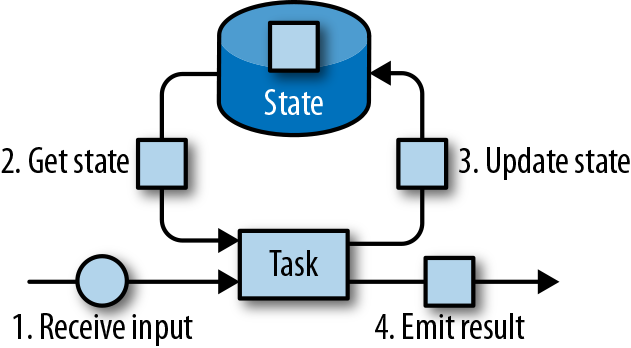
\includegraphics{images/spaf_0310.png}

任务会接收一些输入数据。在处理数据时,任务可以读取和更新状态,并根据输入数据和状态计算结果。最简单的例子,就是统计接收到多少条数据的任务。当任务收到新数据时,它会访问状态以获取当前的计数,然后让计数递增,更新状态并发送出新的计数。

应用程序里,读取和写入状态的逻辑一般都很简单直接,而有效可靠的状态管理会复杂一些。这包括如何处理很大的状态------可能会超过内存,并且保证在发生故障时不会丢失任何状态。幸运的是,Flink会帮我们处理这相关的所有问题,包括状态一致性、故障处理以及高效存储和访问,以便开发人员可以专注于应用程序的逻辑。

在Flink中,状态始终与特定算子相关联。为了使运行时的Flink了解算子的状态,算子需要预先注册其状态。总的说来,有两种类型的状态:算子状态(operator
state)和键控状态(keyed
state),它们有着不同的范围访问,我们将在下面展开讨论。

\hypertarget{ux7b97ux5b50ux72b6ux6001}{%
\subsection{算子状态}\label{ux7b97ux5b50ux72b6ux6001}}

算子状态的作用范围限定为算子任务。这意味着由同一并行任务所处理的所有数据都可以访问到相同的状态,状态对于同一任务而言是共享的。算子状态不能由相同或不同算子的另一个任务访问。图3-11显示了任务如何访问算子状态。

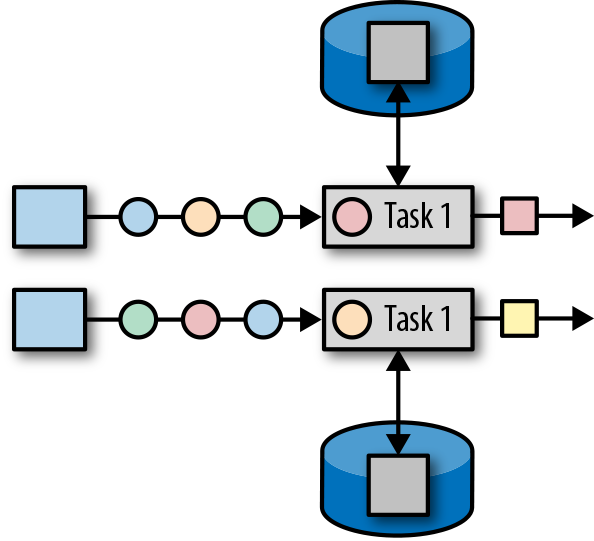
\includegraphics{images/spaf_0311.png}

Flink为算子状态提供三种基本数据结构:

\begin{itemize}
\tightlist
\item
  列表状态:将状态表示为一组数据的列表。
\item
  联合列表状态:也将状态表示为数据的列表。它与常规列表状态的区别在于,在发生故障时,或者从保存点(savepoint)启动应用程序时如何恢复。我们将在后面继续讨论。
\item
  广播状态:如果一个算子有多项任务,而它的每项任务状态又都相同,那么这种特殊情况最适合应用广播状态。在保存检查点和重新调整算子并行度时,会用到这个特性。这两部分内容将在本章后面讨论。
\end{itemize}

\hypertarget{ux952eux63a7ux72b6ux6001}{%
\subsection{键控状态}\label{ux952eux63a7ux72b6ux6001}}

顾名思义,键控状态是根据输入数据流中定义的键(key)来维护和访问的。Flink为每个键值维护一个状态实例,并将具有相同键的所有数据,都分区到同一个算子任务中,这个任务会维护和处理这个key对应的状态。当任务处理一条数据时,它会自动将状态的访问范围限定为当前数据的key。因此,具有相同key的所有数据都会访问相同的状态。图3-12显示了任务如何与键控状态进行交互。

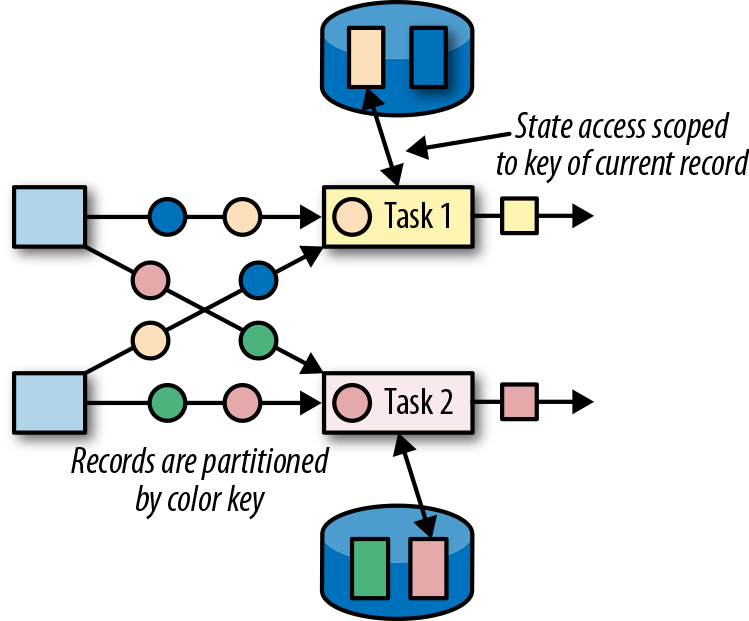
\includegraphics{images/spaf_0312.png}

我们可以将键控状态看成是在算子所有并行任务上,对键进行分区(或分片)之后的一个键值映射(key-value
map)。Flink为键控状态提供不同的数据结构,用于确定map中每个key存储的值的类型。我们简单了解一下最常见的键控状态。

\begin{itemize}
\tightlist
\item
  值状态:为每个键存储一个任意类型的单个值。复杂数据结构也可以存储为值状态。
\item
  列表状态:为每个键存储一个值的列表。列表里的每个数据可以是任意类型。
\item
  映射状态:为每个键存储一个键值映射(map)。map的key和value可以是任意类型。
\end{itemize}

状态的数据结构可以让Flink实现更有效的状态访问。我们将在``在运行时上下文(RuntimeContext)中声明键控状态''中做进一步讨论。

\hypertarget{ux72b6ux6001ux540eux7aef}{%
\subsection{状态后端}\label{ux72b6ux6001ux540eux7aef}}

每传入一条数据,有状态的算子任务都会读取和更新状态。由于有效的状态访问对于处理数据的低延迟至关重要,因此每个并行任务都会在本地维护其状态,以确保快速的状态访问。状态到底是如何被存储、访问以及维护的?这件事由一个可插入的组件决定,这个组件就叫做状态后端(state
backend)。状态后端主要负责两件事:本地的状态管理,以及将检查点(checkpoint)状态写入远程存储。

对于本地状态管理,状态后端会存储所有键控状态,并确保所有的访问都被正确地限定在当前键范围。Flink提供了默认的状态后端,会将键控状态作为内存中的对象进行管理,将它们存储在JVM堆上。另一种状态后端则会把状态对象进行序列化,并将它们放入RocksDB中,然后写入本地硬盘。第一种方式可以提供非常快速的状态访问,但它受内存大小的限制;而访问RocksDB状态后端存储的状态速度会较慢,但其状态可以增长到非常大。

状态检查点的写入也非常重要,这是因为Flink是一个分布式系统,而状态只能在本地维护。TaskManager进程(所有任务在其上运行)可能在任何时间点挂掉。因此,它的本地存储只能被认为是不稳定的。状态后端负责将任务的状态检查点写入远程的持久存储。写入检查点的远程存储可以是分布式文件系统,也可以是数据库。不同的状态后端在状态检查点的写入机制方面有所不同。例如,RocksDB状态后端支持增量的检查点,这对于非常大的状态来说,可以显著减少状态检查点写入的开销。

我们将在``选择状态后端''一节中更详细地讨论不同的状态后端及其优缺点。

\hypertarget{ux8c03ux6574ux6709ux72b6ux6001ux7b97ux5b50ux7684ux5e76ux884cux5ea6}{%
\subsection{调整有状态算子的并行度}\label{ux8c03ux6574ux6709ux72b6ux6001ux7b97ux5b50ux7684ux5e76ux884cux5ea6}}

流应用程序的一个常见要求是,为了增大或较小输入数据的速率,需要灵活地调整算子的并行度。对于无状态算子而言,并行度的调整没有任何问题,但更改有状态算子的并行度显然就没那么简单了,因为它们的状态需要重新分区并分配给更多或更少的并行任务。
Flink支持四种模式来调整不同类型的状态。

具有键控状态的算子通过将键重新分区为更少或更多任务来缩放并行度。不过,并行度调整时任务之间会有一些必要的状态转移。为了提高效率,Flink并不会对单独的key做重新分配,而是用所谓的``键组'\,'(key
group)把键管理起来。键组是key的分区形式,同时也是Flink为任务分配key的方式。图3-13显示了如何在键组中重新分配键控状态。

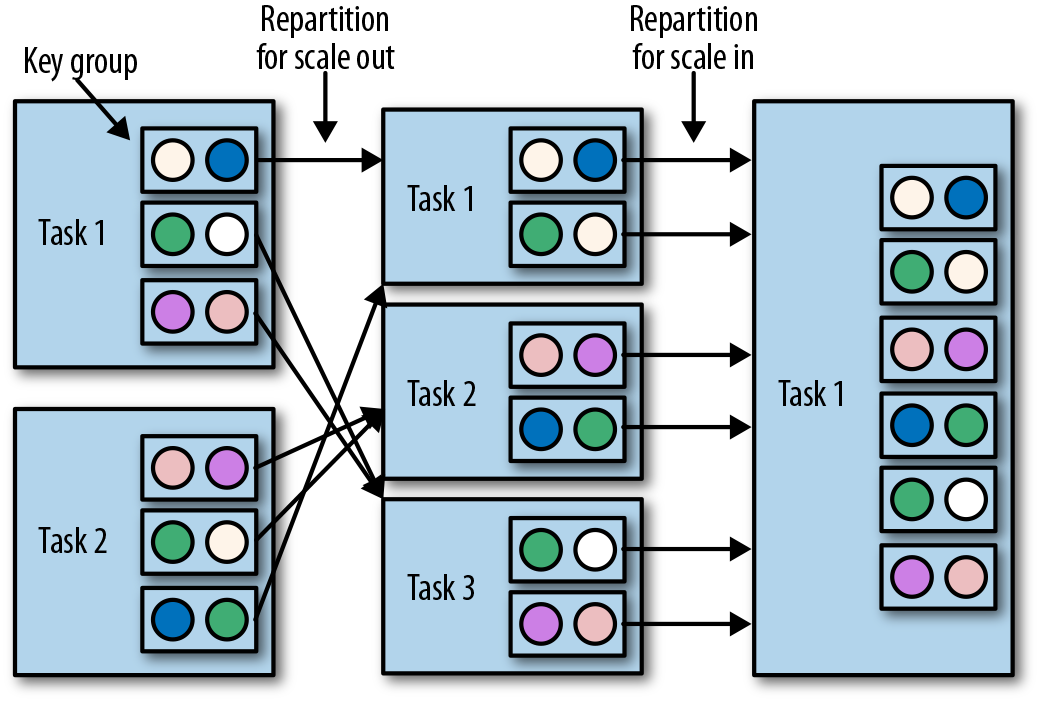
\includegraphics{images/spaf_0313.png}

具有算子列表状态的算子,会通过重新分配列表中的数据项目来进行并行度缩放。从概念上讲,所有并行算子任务的列表项目会被收集起来,并将其均匀地重新分配给更少或更多的任务。如果列表条目少于算子的新并行度,则某些任务将以空状态开始。图3-14显示了算子列表状态的重新分配。

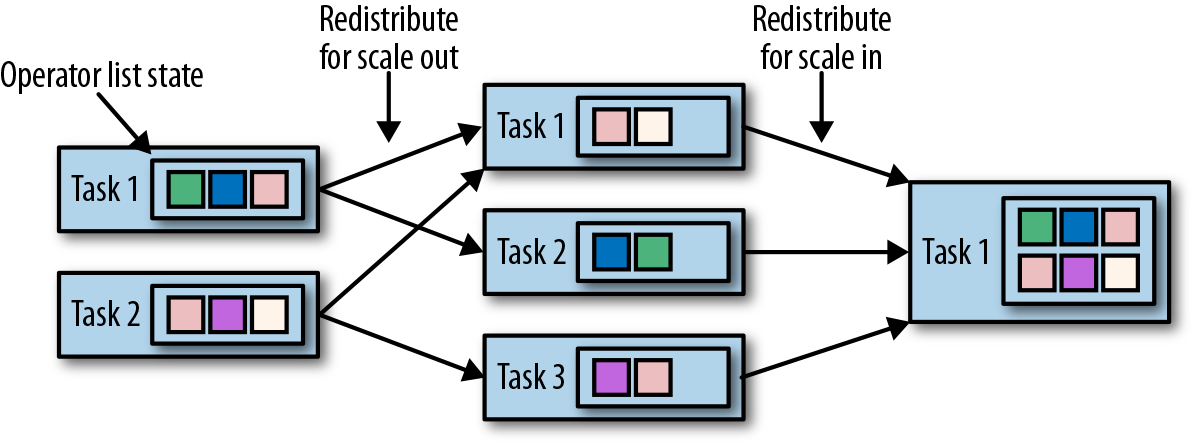
\includegraphics{images/spaf_0314.png}

具有算子联合列表状态的算子,会通过向每个任务广播状态的完整列表,来进行并行度的缩放。然后,任务可以选择要使用的状态项和要丢弃的状态项。图3-15显示了如何重新分配算子联合列表状态。

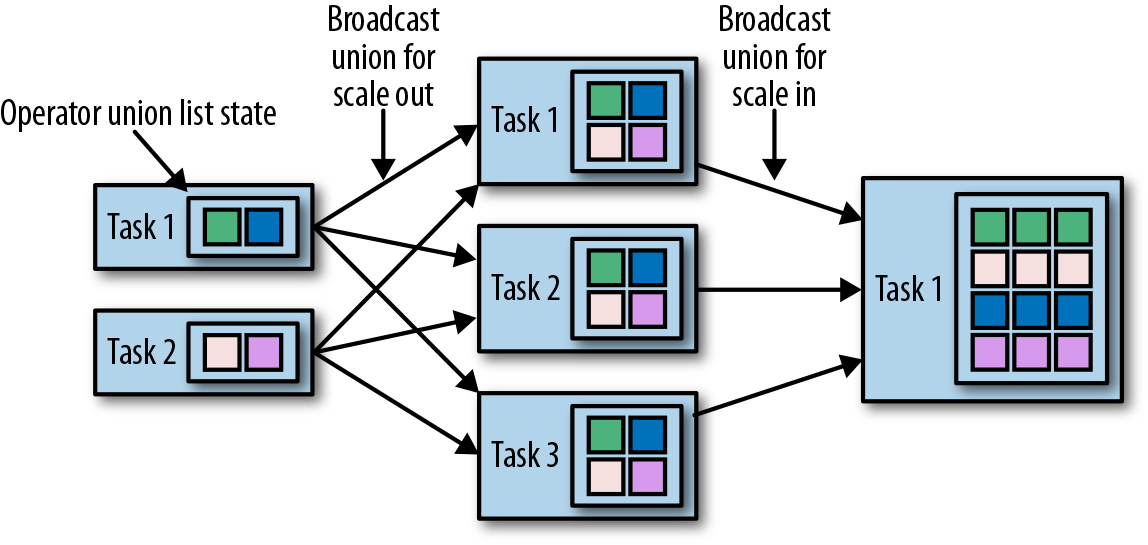
\includegraphics{images/spaf_0315.png}

具有算子广播状态的算子,通过将状态复制到新任务,来增大任务的并行度。这是没问题的,因为广播状态保证了所有任务都具有相同的状态。而对于缩小并行度的情况,我们可以直接取消剩余任务,因为状态是相同的,已经被复制并且不会丢失。图3-16显示了算子广播状态的重新分配。

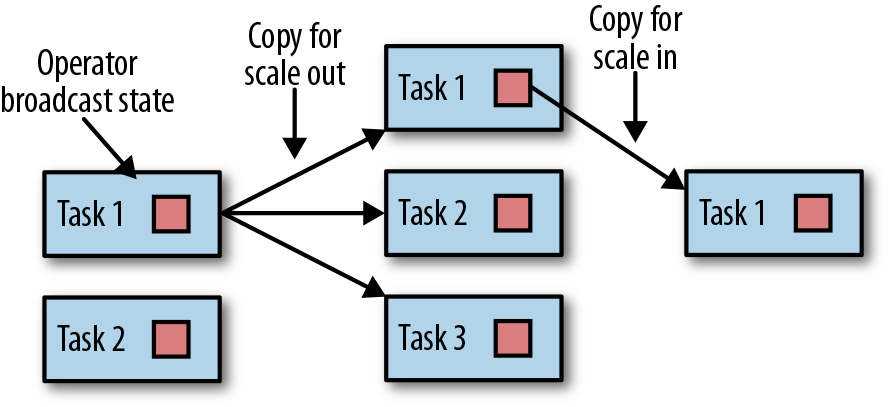
\includegraphics{images/spaf_0316.png}

\hypertarget{ux68c0ux67e5ux70b9ux4fddux5b58ux70b9ux548cux72b6ux6001ux6062ux590d}{%
\section{检查点,保存点和状态恢复}\label{ux68c0ux67e5ux70b9ux4fddux5b58ux70b9ux548cux72b6ux6001ux6062ux590d}}

Flink是一个分布式数据处理系统,因此必须有一套机制处理各种故障,比如被杀掉的进程,故障的机器和中断的网络连接。任务都是在本地维护状态的,所以Flink必须确保状态不会丢失,并且在发生故障时能够保持一致。

在本节中,我们将介绍Flink的检查点(checkpoint)和恢复机制,这保证了``精确一次''(exactly-once)的状态一致性。我们还会讨论Flink独特的保存点(savepoint)功能,这是一个``瑞士军刀''式的工具,可以解决许多操作数据流时面对的问题。

\hypertarget{ux4e00ux81f4ux7684ux68c0ux67e5ux70b9}{%
\subsection{一致的检查点}\label{ux4e00ux81f4ux7684ux68c0ux67e5ux70b9}}

Flink的恢复机制的核心,就是应用状态的一致检查点。有状态流应用的一致检查点,其实就是所有任务状态在某个时间点的一份拷贝,而这个时间点应该是所有任务都恰好处理完一个相同的输入数据的时候。这个过程可以通过一致检查点的一个简单算法步骤来解释。这个算法的步骤是:

\begin{itemize}
\tightlist
\item
  暂停所有输入流的摄取,也就是不再接收新数据的输入。
\item
  等待所有正在处理的数据计算完毕,这意味着结束时,所有任务都已经处理了所有输入数据。
\item
  通过将每个任务的状态复制到远程持久存储,来得到一个检查点。所有任务完成拷贝操作后,检查点就完成了。
\item
  恢复所有输入流的摄取。
\end{itemize}

需要注意,Flink实现的并不是这种简单的机制。我们将在本节后面介绍Flink更精妙的检查点算法。

图3-17显示了一个简单应用中的一致检查点。

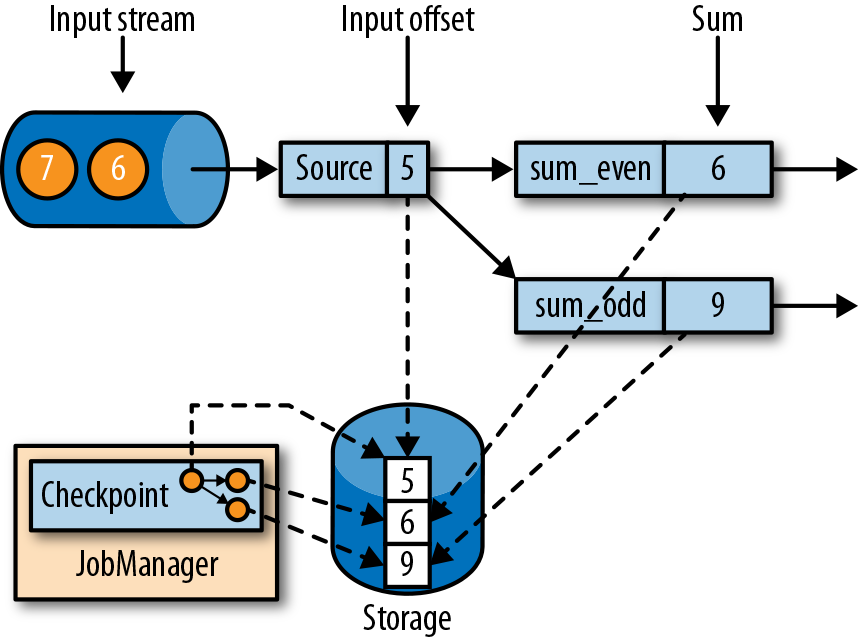
\includegraphics{images/spaf_0317.png}

上面的应用程序中具有单一的输入源(source)任务,输入数据就是一组不断增长的数字的流------1,2,3等。数字流被划分为偶数流和奇数流。求和算子(sum)的两个任务会分别实时计算当前所有偶数和奇数的总和。源任务会将其输入流的当前偏移量存储为状态,而求和任务则将当前的总和值存储为状态。在图3-17中,Flink在输入偏移量为5时,将检查点写入了远程存储,当前的总和为6和9。

\hypertarget{ux4eceux4e00ux81f4ux68c0ux67e5ux70b9ux4e2dux6062ux590dux72b6ux6001}{%
\subsection{从一致检查点中恢复状态}\label{ux4eceux4e00ux81f4ux68c0ux67e5ux70b9ux4e2dux6062ux590dux72b6ux6001}}

在执行流应用程序期间,Flink会定期检查状态的一致检查点。如果发生故障,Flink将会使用最近的检查点来一致恢复应用程序的状态,并重新启动处理流程。图3-18显示了恢复过程。

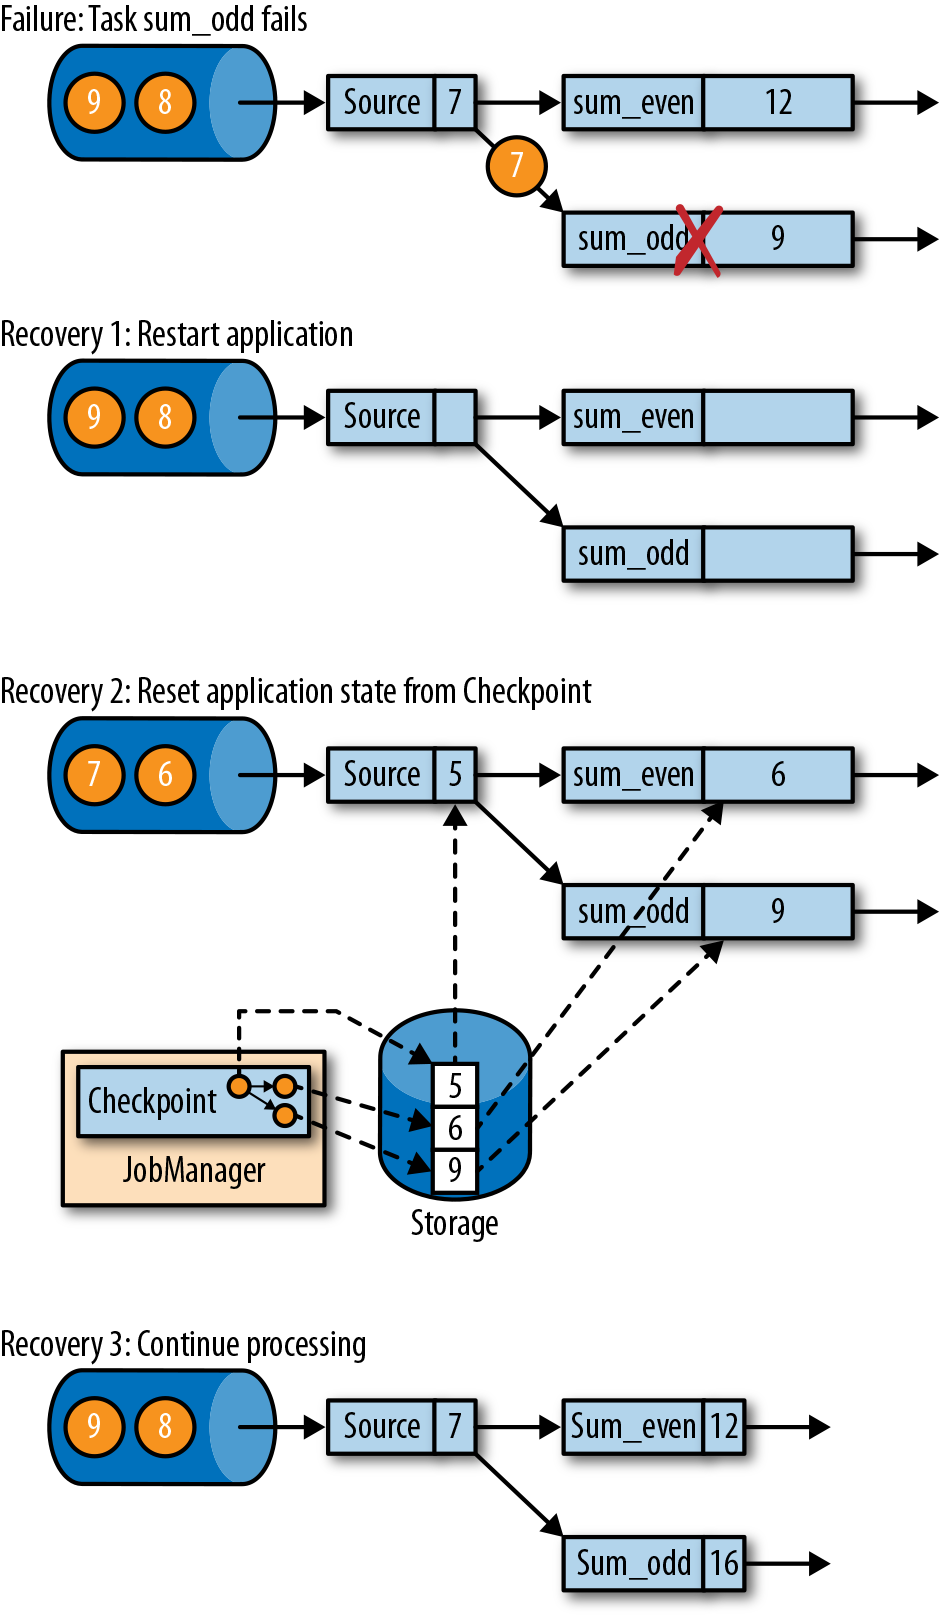
\includegraphics{images/spaf_0318.png}

应用程序从检查点的恢复分为三步:

\begin{itemize}
\tightlist
\item
  重新启动整个应用程序。
\item
  将所有的有状态任务的状态重置为最近一次的检查点。
\item
  恢复所有任务的处理。
\end{itemize}

这种检查点的保存和恢复机制可以为应用程序状态提供``精确一次''(exactly-once)的一致性,因为所有算子都会保存检查点并恢复其所有状态,这样一来所有的输入流就都会被重置到检查点完成时的位置。至于数据源是否可以重置它的输入流,这取决于其实现方式和消费流数据的外部接口。例如,像Apache
Kafka这样的事件日志系统可以提供流上之前偏移位置的数据,所以我们可以将源重置到之前的偏移量,重新消费数据。而从套接字(socket)消费数据的流就不能被重置了,因为套接字的数据一旦被消费就会丢弃掉。因此,对于应用程序而言,只有当所有的输入流消费的都是可重置的数据源时,才能确保在``精确一次''的状态一致性下运行。

从检查点重新启动应用程序后,其内部状态与检查点完成时的状态完全相同。然后它就会开始消费并处理检查点和发生故障之间的所有数据。尽管这意味着Flink会对一些数据处理两次(在故障之前和之后),我们仍然可以说这个机制实现了精确一次的一致性语义,因为所有算子的状态都已被重置,而重置后的状态下还不曾看到这些数据。

我们必须指出,Flink的检查点保存和恢复机制仅仅可以重置流应用程序的内部状态。对于应用中的一些的输出(sink)算子,在恢复期间,某些结果数据可能会多次发送到下游系统,比如事件日志、文件系统或数据库。对于某些存储系统,Flink提供了具有精确一次输出功能的sink函数,比如,可以在检查点完成时提交发出的记录。另一种适用于许多存储系统的方法是幂等更新。在``应用程序一致性保证''一节中,我们还会详细讨论如何解决应用程序端到端的精确一次一致性问题。

\hypertarget{flinkux7684ux68c0ux67e5ux70b9ux7b97ux6cd5}{%
\subsection{Flink的检查点算法}\label{flinkux7684ux68c0ux67e5ux70b9ux7b97ux6cd5}}

Flink的恢复机制,基于它的一致性检查点。前面我们已经了解了从流应用中创建检查点的简单方法------先暂停应用,保存检查点,然后再恢复应用程序,这种方法很好理解,但它的理念是``停止一切'',这对于即使是中等延迟要求的应用程序而言也是不实用的。所以Flink没有这么简单粗暴,而是基于Chandy-Lamport算法实现了分布式快照的检查点保存。该算法并不会暂停整个应用程序,而是将检查点的保存与数据处理分离,这样就可以实现在其它任务做检查点状态保存状态时,让某些任务继续进行而不受影响。接下来我们将解释此算法的工作原理。

Flink的检查点算法用到了一种称为``检查点分界线''(checkpoint
barrier)的特殊数据形式。与水位线(watermark)类似,检查点分界线由source算子注入到常规的数据流中,它的位置是限定好的,不能超过其他数据,也不能被后面的数据超过。检查点分界线带有检查点ID,用来标识它所属的检查点;这样,这个分界线就将一条流逻辑上分成了两部分。分界线之前到来的数据导致的状态更改,都会被包含在当前分界线所属的检查点中;而基于分界线之后的数据导致的所有更改,就会被包含在之后的检查点中。

我们用一个简单的流应用程序作为示例,来一步一步解释这个算法。该应用程序有两个源(source)任务,每个任务都消费一个增长的数字流。源任务的输出被划分为两部分:偶数和奇数的流。每个分区由一个任务处理,该任务计算所有收到的数字的总和,并将更新的总和转发给输出(sink)任务。这个应用程序的结构如图3-19所示。

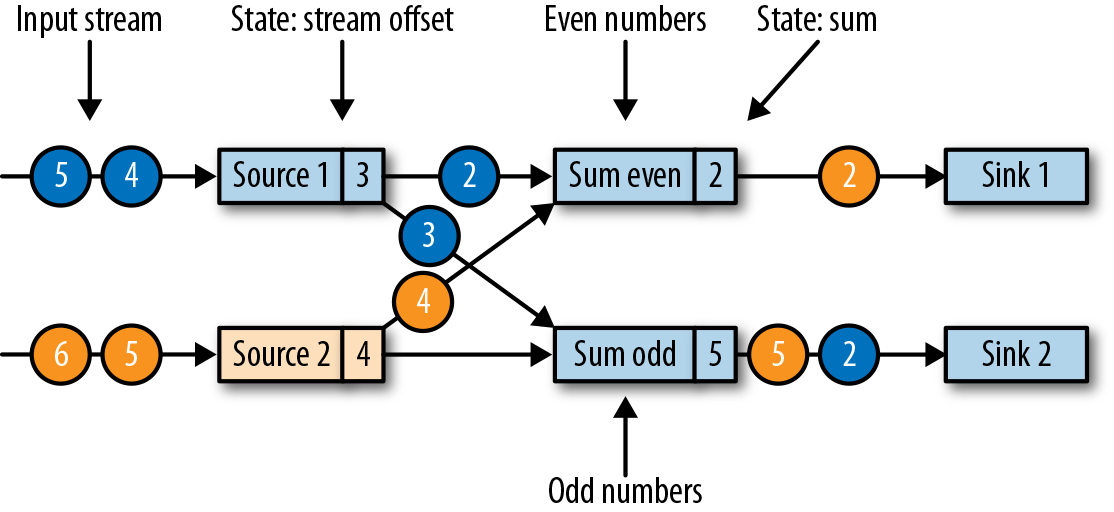
\includegraphics{images/spaf_0319.png}

作业管理器会向每个数据源(source)任务发送一条带有新检查点ID的消息,通过这种方式来启动检查点,如图3-20所示。

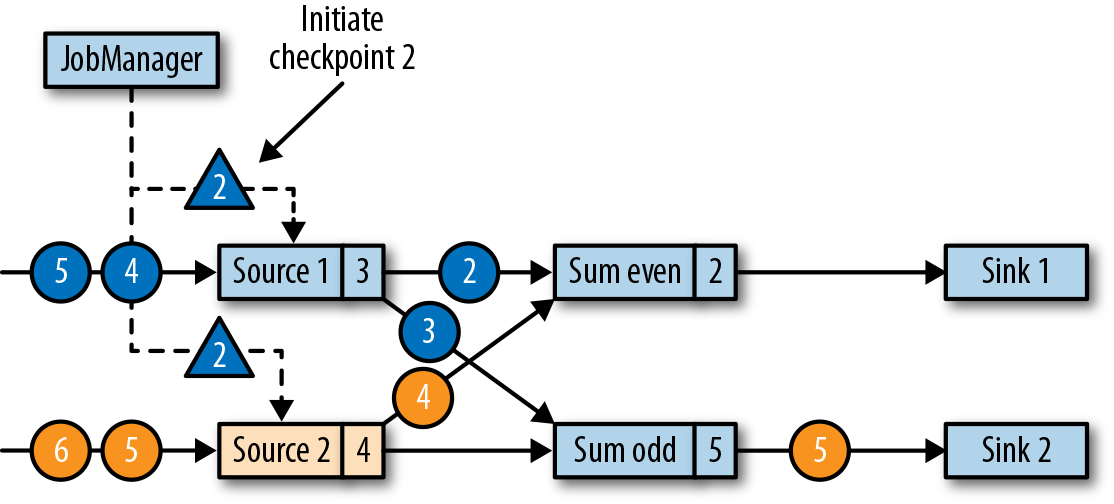
\includegraphics{images/spaf_0320.png}

当source任务收到消息时,它会暂停发出新的数据,在状态后端触发本地状态的检查点保存,并向所有传出的流分区广播带着检查点ID的分界线(barriers)。状态后端在状态检查点完成后会通知任务,而任务会向作业管理器确认检查点完成。在发出所有分界线后,source任务就可以继续常规操作,发出新的数据了。通过将分界线注入到输出流中,源函数(source
function)定义了检查点在流中所处的位置。图3-21显示了两个源任务将本地状态保存到检查点,并发出检查点分界线之后的流应用程序。

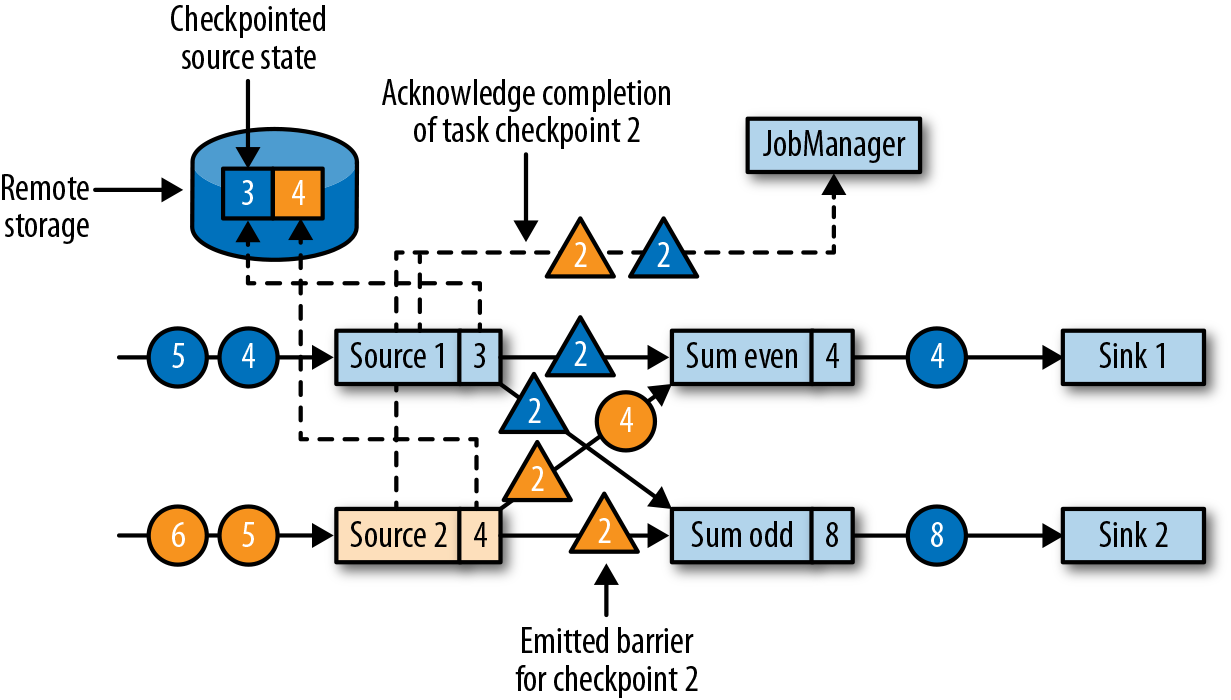
\includegraphics{images/spaf_0321.png}

源任务发出的检查点分界线(barrier),将被传递给所连接的任务。与水位线(watermark)类似,barrier会被广播到所有连接的并行任务,以确保每个任务从它的每个输入流中都能接收到。当任务收到一个新检查点的barrier时,它会等待这个检查点的所有输入分区的barrier到达。在等待的过程中,任务并不会闲着,而是会继续处理尚未提供barrier的流分区中的数据。对于那些barrier已经到达的分区,如果继续有新的数据到达,它们就不会被立即处理,而是先缓存起来。这个等待所有分界线到达的过程,称为``分界线对齐'\,'(barrier
alignment),如图3-22所示。

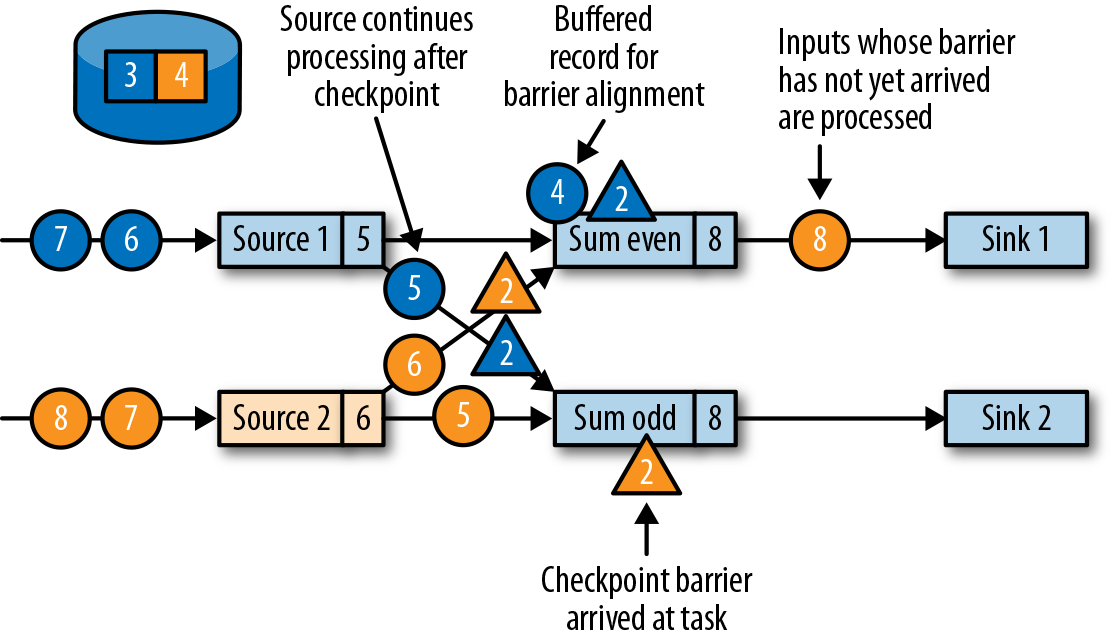
\includegraphics{images/spaf_0322.png}

当任务从所有输入分区都收到barrier时,它就会在状态后端启动一个检查点的保存,并继续向所有下游连接的任务广播检查点分界线,如图3-23所示。

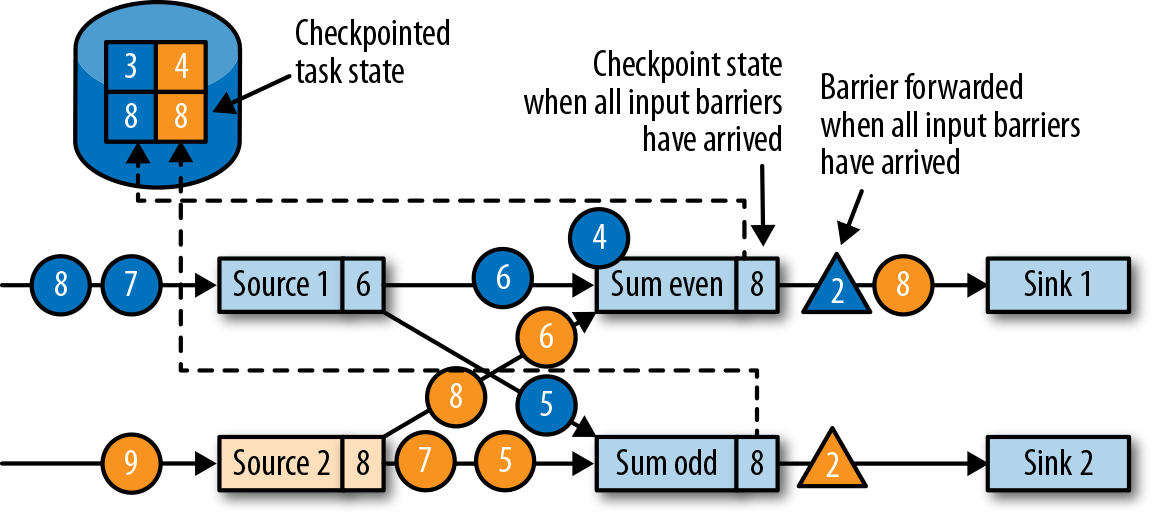
\includegraphics{images/spaf_0323.png}

所有的检查点barrier都发出后,任务就开始处理之前缓冲的数据。在处理并发出所有缓冲数据之后,任务就可以继续正常处理输入流了。图3-24显示了此时的应用程序。

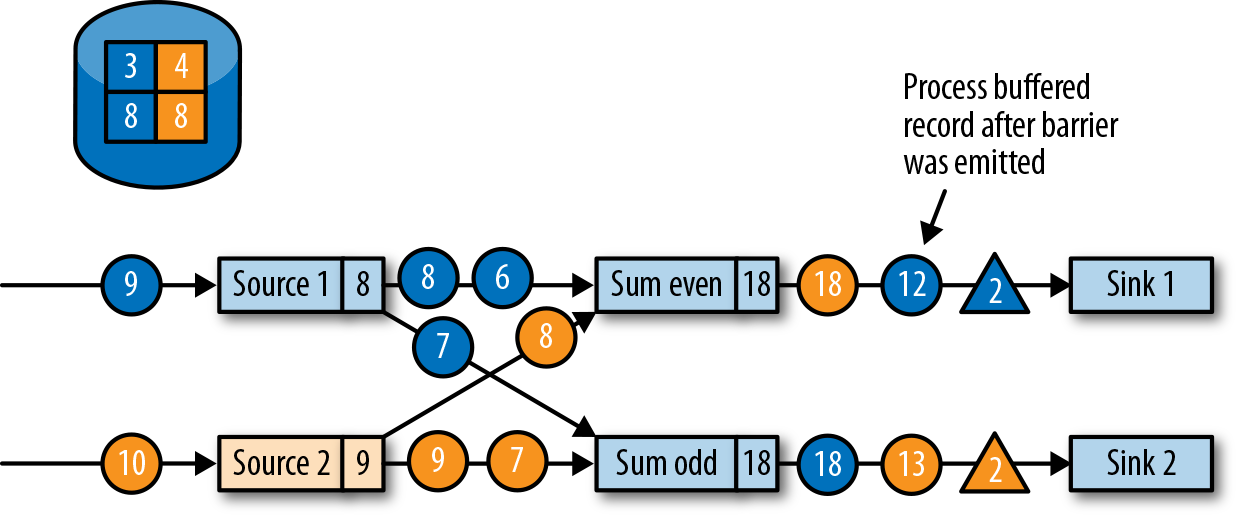
\includegraphics{images/spaf_0324.png}

最终,检查点分界线会到达输出(sink)任务。当sink任务接收到barrier时,它也会先执行``分界线对齐'\,',然后将自己的状态保存到检查点,并向作业管理器确认已接收到barrier。一旦从应用程序的所有任务收到一个检查点的确认信息,作业管理器就会将这个检查点记录为已完成。图3-25显示了检查点算法的最后一步。这样,当发生故障时,我们就可以用已完成的检查点恢复应用程序了。

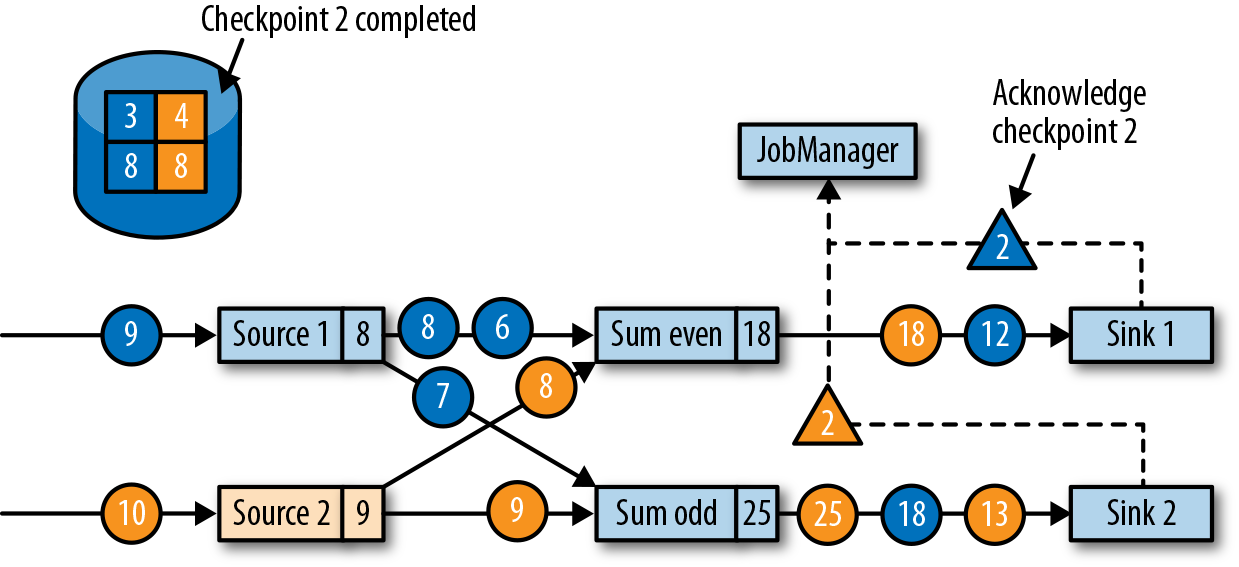
\includegraphics{images/spaf_0325.png}

\hypertarget{ux68c0ux67e5ux70b9ux7684ux6027ux80fdux5f71ux54cd}{%
\subsection{检查点的性能影响}\label{ux68c0ux67e5ux70b9ux7684ux6027ux80fdux5f71ux54cd}}

Flink的检查点算法可以在不停止整个应用程序的情况下,生成一致的分布式检查点。但是,它可能会增加应用程序的处理延迟。Flink对此有一些调整措施,可以在某些场景下显得对性能的影响没那么大。

当任务将其状态保存到检查点时,它其实处于一个阻塞状态,而此时新的输入会被缓存起来。由于状态可能变得非常大,而且检查点需要通过网络将数据写入远程存储系统,检查点的写入很容易就会花费几秒到几分钟的时间------这对于要求低延迟的应用程序而言,显然是不可接受的。在Flink的设计中,真正负责执行检查点写入的,其实是状态后端。具体怎样复制任务的状态,取决于状态后端的实现方式。例如,文件系统(FileSystem)状态后端和RocksDB状态后端都支持了异步(asynchronous)检查点。触发检查点操作时,状态后端会先创建状态的本地副本。本地拷贝完成后,任务就将继续常规的数据处理,这往往并不会花费太多时间。一个后台线程会将本地快照异步复制到远程存储,并在完成检查点后再回来通知任务。异步检查点的机制,显著减少了任务继续处理数据之前的等待时间。此外,RocksDB状态后端还实现了增量的检查点,这样可以大大减少要传输的数据量。

为了减少检查点算法对处理延迟的影响,另一种技术是调整分界线对齐的步骤。对于需要非常低的延迟、并且可以容忍``至少一次''(at-least-once)状态保证的应用程序,Flink可以将检查点算法配置为,在等待barrier对齐期间处理所有到达的数据,而不是把barrier已经到达的那些分区的数据缓存起来。当检查点的所有barrier到达,算子任务就会将状态写入检查点------当然,现在的状态中,就可能包括了一些``提前''的更改,这些更改由本该属于下一个检查点的数据到来时触发。如果发生故障,从检查点恢复时,就将再次处理这些数据:这意味着检查点现在提供的是``至少一次''(at-least-once)而不是``精确一次''(exactly-once)的一致性保证。

\hypertarget{ux4fddux5b58ux70b9}{%
\subsection{保存点}\label{ux4fddux5b58ux70b9}}

Flink的恢复算法是基于状态检查点的。Flink根据可配置的策略,定期保存并自动丢弃检查点。检查点的目的是确保在发生故障时可以重新启动应用程序,所以当应用程序被显式地撤销(cancel)时,检查点会被删除掉。除此之外,应用程序状态的一致性快照还可用于除故障恢复之外的更多功能。

Flink中一个最有价值,也是最独特的功能是保存点(savepoints)。原则上,创建保存点使用的算法与检查点完全相同,因此保存点可以认为就是具有一些额外元数据的检查点。Flink不会自动创建保存点,因此用户(或者外部调度程序)必须明确地触发创建操作。同样,Flink也不会自动清理保存点。第10章将会具体介绍如何触发和处理保存点。

\textbf{使用保存点}

有了应用程序和与之兼容的保存点,我们就可以从保存点启动应用程序了。这会将应用程序的状态初始化为保存点的状态,并从保存点创建时的状态开始运行应用程序。虽然看起来这种行为似乎与用检查点从故障中恢复应用程序完全相同,但实际上故障恢复只是一种特殊情况,它只是在相同的集群上以相同的配置启动相同的应用程序。而从保存点启动应用程序会更加灵活,这就可以让我们做更多事情了。

\begin{itemize}
\tightlist
\item
  可以从保存点启动不同但兼容的应用程序。这样一来,我们就可以及时修复应用程序中的逻辑bug,并让流式应用的源尽可能多地提供之前发生的事件,然后重新处理,以便修复之前的计算结果。修改后的应用程序还可用于运行A
  /
  B测试,或者具有不同业务逻辑的假设场景。这里要注意,应用程序和保存点必须兼容才可以这么做------也就是说,应用程序必须能够加载保存点的状态。
\item
  可以使用不同的并行度来启动相同的应用程序,可以将应用程序的并行度增大或减小。
\item
  可以在不同的集群上启动同样的应用程序。这非常有意义,意味着我们可以将应用程序迁移到较新的Flink版本或不同的集群上去。
\item
  可以使用保存点暂停应用程序,稍后再恢复。这样做的意义在于,可以为更高优先级的应用程序释放集群资源,或者在输入数据不连续生成时释放集群资源。
\item
  还可以将保存点设置为某一版本,并归档(archive)存储应用程序的状态。
\end{itemize}

保存点是非常强大的功能,所以许多用户会定期创建保存点以便能够及时退回之前的状态。我们见到的各种场景中,保存点一个最有趣的应用是不断将流应用程序迁移到更便宜的数据中心上去。

\textbf{从保存点启动应用程序}

前面提到的保存点的所有用例,都遵循相同的模式。那就是首先创建正在运行的应用程序的保存点,然后在一个新启动的应用程序中用它来恢复状态。之前我们已经知道,保存点的创建和检查点非常相似,而接下来我们就将介绍对于一个从保存点启动的应用程序,Flink如何初始化其状态。

应用程序由多个算子组成。每个算子可以定义一个或多个键控状态和算子状态。算子由一个或多个算子任务并行执行。因此,一个典型的应用程序会包含多个状态,这些状态分布在多个算子任务中,这些任务可以运行在不同的TaskManager进程上。

图3-26显示了一个具有三个算子的应用程序,每个算子执行两个算子任务。一个算子(OP-1)具有单一的算子状态(OS-1),而另一个算子(OP-2)具有两个键控状态(KS-1和KS-2)。当保存点创建时,会将所有任务的状态复制到持久化的存储位置。

保存点中的状态拷贝会以算子标识符(operator ID)和状态名称(state
name)组织起来。算子ID和状态名称必须能够将保存点的状态数据,映射到一个正在启动的应用程序的算子状态。从保存点启动应用程序时,Flink会将保存点的数据重新分配给相应的算子任务。

\begin{quote}
请注意,保存点不包含有关算子任务的信息。这是因为当应用程序以不同的并行度启动时,任务数量可能会更改。
\end{quote}

如果我们要从保存点启动一个修改过的应用程序,那么保存点中的状态只能映射到符合标准的应用程序------它里面的算子必须具有相应的ID和状态名称。默认情况下,Flink会自动分配唯一的算子ID。然而,一个算子的ID,是基于它之前算子的ID确定性地生成的。因此,算子的ID会在其前序算子改变时改变,比如,当我们添加了新的或移除掉一个算子时,前序算子ID改变,当前算子ID就会变化。所以对于具有默认算子ID的应用程序而言,如果想在不丢失状态的前提下升级,就会受到极大的限制。因此,我们强烈建议在程序中为算子手动分配唯一ID,而不是依靠Flink的默认分配。我们将在``指定唯一的算子标识符''一节中详细说明如何分配算子标识符。

\hypertarget{flink-datastream-api}{%
\chapter{Flink DataStream API}\label{flink-datastream-api}}

本章介绍了Flink DataStream
API的基本知识。我们展示了典型的Flink流处理程序的结构和组成部分,还讨论了Flink的类型系统以及支持的数据类型,还展示了数据和分区转换操作。窗口操作符,基于时间语义的转换操作,有状态的操作符,以及和外部系统的连接器将在接下来的章节进行介绍。阅读完这一章后,我们将会知道如何去实现一个具有基本功能的流处理程序。我们的示例程序采用Java语言,因为Java语言比较常用。

\hypertarget{ux4f60ux597dflink}{%
\section{你好,Flink!}\label{ux4f60ux597dflink}}

让我们写一个简单的例子来获得使用DataStream
API编写流处理应用程序的粗浅印象。我们将使用这个简单的示例来展示一个Flink程序的基本结构,以及介绍一些DataStream
API的重要特性。我们的示例程序摄取了一条(来自多个传感器的)温度测量数据流。

首先让我们看一下表示传感器读数的数据结构:

\begin{Shaded}
\begin{Highlighting}[]
\KeywordTok{public} \KeywordTok{class}\NormalTok{ SensorReading \{}

    \KeywordTok{public} \BuiltInTok{String}\NormalTok{ id;}
    \KeywordTok{public} \DataTypeTok{long}\NormalTok{ timestamp;}
    \KeywordTok{public} \DataTypeTok{double}\NormalTok{ temperature;}

    \KeywordTok{public} \FunctionTok{SensorReading}\NormalTok{() \{ \}}

    \KeywordTok{public} \FunctionTok{SensorReading}\NormalTok{(}\BuiltInTok{String}\NormalTok{ id, }\DataTypeTok{long}\NormalTok{ timestamp, }\DataTypeTok{double}\NormalTok{ temperature) \{}
        \KeywordTok{this}\NormalTok{.}\FunctionTok{id}\NormalTok{ = id;}
        \KeywordTok{this}\NormalTok{.}\FunctionTok{timestamp}\NormalTok{ = timestamp;}
        \KeywordTok{this}\NormalTok{.}\FunctionTok{temperature}\NormalTok{ = temperature;}
\NormalTok{    \}}

    \KeywordTok{public} \BuiltInTok{String} \FunctionTok{toString}\NormalTok{() \{}
        \KeywordTok{return} \StringTok{"("}\NormalTok{ + }\KeywordTok{this}\NormalTok{.}\FunctionTok{id}\NormalTok{ + }\StringTok{", "}\NormalTok{ + }\KeywordTok{this}\NormalTok{.}\FunctionTok{timestamp}\NormalTok{ + }\StringTok{", "}\NormalTok{ + }\KeywordTok{this}\NormalTok{.}\FunctionTok{temperature}\NormalTok{ + }\StringTok{")"}\NormalTok{;}
\NormalTok{    \}}
\NormalTok{\}}
\end{Highlighting}
\end{Shaded}

示例程序将温度从华氏温度读数转换成摄氏温度读数,然后针对每一个传感器,每5秒钟计算一次平均温度纸。

\begin{Shaded}
\begin{Highlighting}[]
\KeywordTok{public} \KeywordTok{class}\NormalTok{ AverageSensorReadings \{}
  \KeywordTok{public} \DataTypeTok{static} \DataTypeTok{void} \FunctionTok{main}\NormalTok{(}\BuiltInTok{String}\NormalTok{[] args) }\KeywordTok{throws} \BuiltInTok{Exception}\NormalTok{ \{}
    \DataTypeTok{final}\NormalTok{ StreamExecutionEnvironment env = StreamExecutionEnvironment.}\FunctionTok{getExecutionEnvironment}\NormalTok{();}

\NormalTok{    DataStream\textless{}SensorReading\textgreater{} sensorData = env.}\FunctionTok{addSource}\NormalTok{(}\KeywordTok{new} \FunctionTok{SensorSource}\NormalTok{());}

\NormalTok{    DataStream\textless{}T\textgreater{} avgTemp = sensorData}
\NormalTok{      .}\FunctionTok{map}\NormalTok{(r {-}\textgreater{} \{}
        \BuiltInTok{Double}\NormalTok{ celsius = (r.}\FunctionTok{temperature}\NormalTok{ {-} }\DecValTok{32}\NormalTok{) * (}\FloatTok{5.}\DecValTok{0}\NormalTok{ / }\FloatTok{9.}\DecValTok{0}\NormalTok{);}
        \KeywordTok{return} \FunctionTok{SensorReading}\NormalTok{(r.}\FunctionTok{id}\NormalTok{, r.}\FunctionTok{timestamp}\NormalTok{, celsius);}
\NormalTok{      \})}
\NormalTok{      .}\FunctionTok{keyBy}\NormalTok{(r {-}\textgreater{} r.}\FunctionTok{id}\NormalTok{)}
\NormalTok{      .}\FunctionTok{window}\NormalTok{(}\FunctionTok{TumblingProcessingTimeWindows}\NormalTok{(}\BuiltInTok{Time}\NormalTok{.}\FunctionTok{seconds}\NormalTok{(}\DecValTok{5}\NormalTok{)))}
\NormalTok{      .}\FunctionTok{apply}\NormalTok{(}\KeywordTok{new} \FunctionTok{TemperatureAverager}\NormalTok{());}

\NormalTok{    avgTemp.}\FunctionTok{print}\NormalTok{();}

\NormalTok{    env.}\FunctionTok{execute}\NormalTok{(}\StringTok{"Compute average sensor temperature"}\NormalTok{);}
\NormalTok{  \}}
\NormalTok{\}}
\end{Highlighting}
\end{Shaded}

你可能已经注意到Flink程序的定义和提交执行使用的就是正常的Java的方法。大多数情况下,这些代码都写在一个静态main方法中。在我们的例子中,我们定义了AverageSensorReadings对象,然后将大多数的应用程序逻辑放在了main()中。

Flink流处理程序的结构如下:

\begin{enumerate}
\def\labelenumi{\arabic{enumi}.}
\tightlist
\item
  创建Flink程序执行环境。
\item
  从数据源读取一条或者多条流数据
\item
  使用流转换算子实现业务逻辑
\item
  将计算结果输出到一个或者多个外部设备(可选)
\item
  执行程序
\end{enumerate}

接下来我们详细的学习一下这些部分。

\hypertarget{ux642dux5efaux6267ux884cux73afux5883}{%
\section{搭建执行环境}\label{ux642dux5efaux6267ux884cux73afux5883}}

编写Flink程序的第一件事情就是搭建执行环境。执行环境决定了程序是运行在单机上还是集群上。在DataStream
API中,程序的执行环境是由StreamExecutionEnvironment设置的。在我们的例子中,我们通过调用静态getExecutionEnvironment()方法来获取执行环境。这个方法根据调用方法的上下文,返回一个本地的或者远程的环境。如果这个方法是一个客户端提交到远程集群的代码调用的,那么这个方法将会返回一个远程的执行环境。否则,将返回本地执行环境。

也可以用下面的方法来显式的创建本地或者远程执行环境:

\begin{Shaded}
\begin{Highlighting}[]
\NormalTok{StreamExecutionEnvironment localEnv = StreamExecutionEnvironment}
\NormalTok{  .}\FunctionTok{createLocalEnvironment}\NormalTok{();}

\NormalTok{StreamExecutionEnvironment remoteEnv = StreamExecutionEnvironment}
\NormalTok{  .}\FunctionTok{createRemoteEnvironment}\NormalTok{(}
    \StringTok{"host"}\NormalTok{, }\CommentTok{// hostname of JobManager}
    \DecValTok{1234}\NormalTok{, }\CommentTok{// port of JobManager process}
    \StringTok{"path/to/jarFile.jar"}
\NormalTok{  ); }\CommentTok{// JAR file to ship to the JobManager}
\end{Highlighting}
\end{Shaded}

执行环境提供了很多配置选项,例如:设置程序的并行度和程序是否开启容错机制。

\hypertarget{ux8bfbux53d6ux8f93ux5165ux6d41}{%
\section{读取输入流}\label{ux8bfbux53d6ux8f93ux5165ux6d41}}

一旦执行环境设置好,就该写业务逻辑了。StreamExecutionEnvironment提供了创建数据源的方法,这些方法可以从数据流中将数据摄取到程序中。数据流可以来自消息队列或者文件系统,也可能是实时产生的(例如socket)。

在我们的例子里面,我们这样写:

\begin{Shaded}
\begin{Highlighting}[]
\NormalTok{DataStream\textless{}SensorReading\textgreater{} sensorData = env}
\NormalTok{  .}\FunctionTok{addSource}\NormalTok{(}\KeywordTok{new} \FunctionTok{SensorSource}\NormalTok{());}
\end{Highlighting}
\end{Shaded}

这样就可以连接到传感器测量数据的数据源并创建一个类型为SensorReading的DataStream了。Flink支持很多数据类型,我们将在接下来的章节里面讲解。在我们的例子里面,我们的数据类型是一个定义好的Java
POJO类。SensorReading样例类包含了传感器ID,数据的测量时间戳,以及测量温度值。assignTimestampsAndWatermarks(new
SensorTimeAssigner)方法指定了如何设置事件时间语义的时间戳和水位线。有关SensorTimeAssigner我们后面再讲。

\hypertarget{ux8f6cux6362ux7b97ux5b50ux7684ux4f7fux7528}{%
\section{转换算子的使用}\label{ux8f6cux6362ux7b97ux5b50ux7684ux4f7fux7528}}

一旦我们有一条DataStream,我们就可以在这条数据流上面使用转换算子了。转换算子有很多种。一些转换算子可以产生一条新的DataStream,当然这个DataStream的类型可能是新类型。还有一些转换算子不会改变原有DataStream的数据,但会将数据流分区或者分组。业务逻辑就是由转换算子串起来组合而成的。

在我们的例子中,我们首先使用map()转换算子将传感器的温度值转换成了摄氏温度单位。然后,我们使用keyBy()转换算子将传感器读数流按照传感器ID进行分区。接下来,我们定义了一个window()算子,这个算子将每个传感器ID所对应的分区的传感器读数分配到了5秒钟的滚动窗口中。

\begin{Shaded}
\begin{Highlighting}[]
\NormalTok{DataStream\textless{}T\textgreater{} avgTemp = sensorData}
\NormalTok{  .}\FunctionTok{map}\NormalTok{(r {-}\textgreater{} \{}
    \BuiltInTok{Double}\NormalTok{ celsius = (r.}\FunctionTok{temperature}\NormalTok{ {-}}\DecValTok{32}\NormalTok{) * (}\FloatTok{5.}\DecValTok{0}\NormalTok{ / }\FloatTok{9.}\DecValTok{0}\NormalTok{);}
    \KeywordTok{return} \FunctionTok{SensorReading}\NormalTok{(r.}\FunctionTok{id}\NormalTok{, r.}\FunctionTok{timestamp}\NormalTok{, celsius);}
\NormalTok{  \})}
\NormalTok{  .}\FunctionTok{keyBy}\NormalTok{(r {-}\textgreater{} r.}\FunctionTok{id}\NormalTok{)}
\NormalTok{  .}\FunctionTok{window}\NormalTok{(}\FunctionTok{TumblingProcessingTimeWindows}\NormalTok{(}\BuiltInTok{Time}\NormalTok{.}\FunctionTok{seconds}\NormalTok{(}\DecValTok{5}\NormalTok{)))}
\NormalTok{  .}\FunctionTok{apply}\NormalTok{(}\KeywordTok{new} \FunctionTok{TemperatureAverager}\NormalTok{());}
\end{Highlighting}
\end{Shaded}

窗口转换算子将在``窗口操作符''一章中讲解。最后,我们使用了一个UDF函数来计算每个窗口的温度的平均值。我们稍后将会讨论UDF函数的实现。

\hypertarget{ux8f93ux51faux7ed3ux679c}{%
\section{输出结果}\label{ux8f93ux51faux7ed3ux679c}}

流处理程序经常将它们的计算结果发送到一些外部系统中去,例如:Apache
Kafka,文件系统,或者数据库中。Flink提供了一个维护的很好的sink算子的集合,这些sink算子可以用来将数据写入到不同的系统中去。我们也可以实现自己的sink算子。也有一些Flink程序并不会向第三方外部系统发送数据,而是将数据存储到Flink系统内部,然后可以使用Flink的可查询状态的特性来查询数据。

在我们的例子中,计算结果是一个\texttt{DataStream\textless{}SensorReading\textgreater{}}数据记录。每一条数据记录包含了一个传感器在5秒钟的周期里面的平均温度。计算结果组成的数据流将会调用print()将计算结果写到标准输出。

\begin{Shaded}
\begin{Highlighting}[]
\NormalTok{avgTemp.}\FunctionTok{print}\NormalTok{();}
\end{Highlighting}
\end{Shaded}

\begin{quote}
要注意一点,流的Sink算子的选择将会影响应用程序端到端(end-to-end)的一致性,具体就是应用程序的计算提供的到底是at-least-once还是exactly-once的一致性语义。应用程序端到端的一致性依赖于所选择的流的Sink算子和Flink的检查点算法的集成使用。
\end{quote}

\hypertarget{ux6267ux884c}{%
\section{执行}\label{ux6267ux884c}}

当应用程序完全写好时,我们可以调用StreamExecutionEnvironment.execute()来执行应用程序。在我们的例子中就是我们的最后一行调用:

\begin{Shaded}
\begin{Highlighting}[]
\NormalTok{env.}\FunctionTok{execute}\NormalTok{(}\StringTok{"Compute average sensor temperature"}\NormalTok{);}
\end{Highlighting}
\end{Shaded}

Flink程序是惰性执行的。也就是说创建数据源和转换算子的API调用并不会立刻触发任何数据处理逻辑。API调用仅仅是在执行环境中构建了一个执行计划,这个执行计划包含了执行环境创建的数据源和所有的将要用在数据源上的转换算子。只有当execute()被调用时,系统才会触发程序的执行。

构建好的执行计划将被翻译成一个JobGraph并提交到JobManager上面去执行。根据执行环境的种类,一个JobManager将会运行在一个本地线程中(如果是本地执行环境的化)或者JobGraph将会被发送到一个远程的JobManager上面去。如果JobManager远程运行,那么JobGraph必须和一个包含有所有类和应用程序的依赖的JAR包一起发送到远程JobManager。

\hypertarget{ux81eaux5b9aux4e49ux4ea7ux751fux4f20ux611fux5668ux8bfbux6570ux7684ux6570ux636eux6e90}{%
\section{自定义产生传感器读数的数据源}\label{ux81eaux5b9aux4e49ux4ea7ux751fux4f20ux611fux5668ux8bfbux6570ux7684ux6570ux636eux6e90}}

\begin{Shaded}
\begin{Highlighting}[]
\KeywordTok{public} \KeywordTok{class}\NormalTok{ SensorSource }\KeywordTok{extends}\NormalTok{ RichParallelSourceFunction\textless{}SensorReading\textgreater{} \{}

    \KeywordTok{private} \DataTypeTok{boolean}\NormalTok{ running = }\KeywordTok{true}\NormalTok{;}

    \AttributeTok{@Override}
    \KeywordTok{public} \DataTypeTok{void} \FunctionTok{run}\NormalTok{(SourceContext\textless{}SensorReading\textgreater{} srcCtx) }\KeywordTok{throws} \BuiltInTok{Exception}\NormalTok{ \{}

        \BuiltInTok{Random}\NormalTok{ rand = }\KeywordTok{new} \BuiltInTok{Random}\NormalTok{();}

        \BuiltInTok{String}\NormalTok{[] sensorIds = }\KeywordTok{new} \BuiltInTok{String}\NormalTok{[}\DecValTok{10}\NormalTok{];}
        \DataTypeTok{double}\NormalTok{[] curFTemp = }\KeywordTok{new} \DataTypeTok{double}\NormalTok{[}\DecValTok{10}\NormalTok{];}
        \KeywordTok{for}\NormalTok{ (}\DataTypeTok{int}\NormalTok{ i = }\DecValTok{0}\NormalTok{; i \textless{} }\DecValTok{10}\NormalTok{; i++) \{}
\NormalTok{            sensorIds[i] = }\StringTok{"sensor\_"}\NormalTok{ + i;}
\NormalTok{            curFTemp[i] = }\DecValTok{65}\NormalTok{ + (rand.}\FunctionTok{nextGaussian}\NormalTok{() * }\DecValTok{20}\NormalTok{);}
\NormalTok{        \}}

        \KeywordTok{while}\NormalTok{ (running) \{}
            \DataTypeTok{long}\NormalTok{ curTime = }\BuiltInTok{Calendar}\NormalTok{.}\FunctionTok{getInstance}\NormalTok{().}\FunctionTok{getTimeInMillis}\NormalTok{();}
            \KeywordTok{for}\NormalTok{ (}\DataTypeTok{int}\NormalTok{ i = }\DecValTok{0}\NormalTok{; i \textless{} }\DecValTok{10}\NormalTok{; i++) \{}
\NormalTok{                curFTemp[i] += rand.}\FunctionTok{nextGaussian}\NormalTok{() * }\FloatTok{0.}\DecValTok{5}\NormalTok{;}
\NormalTok{                srcCtx.}\FunctionTok{collect}\NormalTok{(}\KeywordTok{new} \FunctionTok{SensorReading}\NormalTok{(sensorIds[i], curTime, curFTemp[i]));}
\NormalTok{            \}}

            \BuiltInTok{Thread}\NormalTok{.}\FunctionTok{sleep}\NormalTok{(}\DecValTok{100}\NormalTok{);}
\NormalTok{        \}}
\NormalTok{    \}}

    \AttributeTok{@Override}
    \KeywordTok{public} \DataTypeTok{void} \FunctionTok{cancel}\NormalTok{() \{}
        \KeywordTok{this}\NormalTok{.}\FunctionTok{running}\NormalTok{ = }\KeywordTok{false}\NormalTok{;}
\NormalTok{    \}}
\NormalTok{\}}
\end{Highlighting}
\end{Shaded}

使用方法

\begin{Shaded}
\begin{Highlighting}[]
\NormalTok{DataStream\textless{}SensorReading\textgreater{} sensorData = env.}\FunctionTok{addSource}\NormalTok{(}\KeywordTok{new} \FunctionTok{SensorSource}\NormalTok{());}
\end{Highlighting}
\end{Shaded}

\hypertarget{ux8f6cux6362ux7b97ux5b50-1}{%
\section{转换算子}\label{ux8f6cux6362ux7b97ux5b50-1}}

在这一小节我们将大概看一下DataStream
API的基本转换算子。与时间有关的操作符(例如窗口操作符和其他特殊的转换算子)将会在后面的章节叙述。一个流的转换操作将会应用在一个或者多个流上面,这些转换操作将流转换成一个或者多个输出流。编写一个DataStream
API简单来说就是将这些转换算子组合在一起来构建一个数据流图,这个数据流图就实现了我们的业务逻辑。

大部分的流转换操作都基于用户自定义函数UDF。UDF函数打包了一些业务逻辑并定义了输入流的元素如何转换成输出流的元素。像MapFunction这样的函数,将会被定义为类,这个类实现了Flink针对特定的转换操作暴露出来的接口。

\begin{Shaded}
\begin{Highlighting}[]
\NormalTok{DataStream\textless{}}\BuiltInTok{String}\NormalTok{\textgreater{} sensorIds = filteredReadings.}\FunctionTok{map}\NormalTok{(r {-}\textgreater{} r.}\FunctionTok{id}\NormalTok{);}
\end{Highlighting}
\end{Shaded}

函数接口定义了需要由用户实现的转换方法,例如上面例子中的map()方法。

大部分函数接口被设计为Single Abstract
Method(单独抽象方法)接口,并且接口可以使用Java 8匿名函数来实现。Java
DataStream API也内置了对匿名函数的支持。当讲解DataStream
API的转换算子时,我们展示了针对所有函数类的接口,但为了简洁,大部分接口的实现使用匿名函数而不是函数类的方式。

DataStream
API针对大多数数据转换操作提供了转换算子。如果你很熟悉批处理API、函数式编程语言或者SQL,那么你将会发现这些API很容易学习。我们会将DataStream
API的转换算子分成四类:

\begin{itemize}
\tightlist
\item
  基本转换算子:将会作用在数据流中的每一条单独的数据上。
\item
  KeyedStream转换算子:在数据有key的情况下,对数据应用转换算子。
\item
  多流转换算子:合并多条流为一条流或者将一条流分割为多条流。
\item
  分布式转换算子:将重新组织流里面的事件。
\end{itemize}

\hypertarget{ux57faux672cux8f6cux6362ux7b97ux5b50}{%
\subsection{基本转换算子}\label{ux57faux672cux8f6cux6362ux7b97ux5b50}}

基本转换算子会针对流中的每一个单独的事件做处理,也就是说每一个输入数据会产生一个输出数据。单值转换,数据的分割,数据的过滤,都是基本转换操作的典型例子。我们将解释这些算子的语义并提供示例代码。

\emph{MAP}

map算子通过调用DataStream.map()来指定。map算子的使用将会产生一条新的数据流。它会将每一个输入的事件传送到一个用户自定义的mapper,这个mapper只返回一个输出事件,这个输出事件和输入事件的类型可能不一样。图5-1展示了一个map算子,这个map将每一个正方形转化成了圆形。

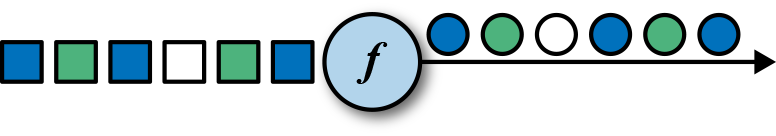
\includegraphics{images/spaf_0501.png}

MapFunction的类型与输入事件和输出事件的类型相关,可以通过实现MapFunction接口来定义。接口包含map()函数,这个函数将一个输入事件恰好转换为一个输出事件。

\begin{Shaded}
\begin{Highlighting}[]
\CommentTok{// T: the type of input elements}
\CommentTok{// O: the type of output elements}
\NormalTok{MapFunction[T, O]}
\NormalTok{    \textgreater{} }\FunctionTok{map}\NormalTok{(T): O}
\end{Highlighting}
\end{Shaded}

下面的代码实现了将SensorReading中的id字段抽取出来的功能。

\begin{Shaded}
\begin{Highlighting}[]
\NormalTok{DataStream\textless{}SensorReading\textgreater{} readings = ...}
\NormalTok{DataStream\textless{}}\BuiltInTok{String}\NormalTok{\textgreater{} sensorIds = readings.}\FunctionTok{map}\NormalTok{(}\KeywordTok{new} \FunctionTok{IdExtractor}\NormalTok{());}

\KeywordTok{public} \DataTypeTok{static} \KeywordTok{class}\NormalTok{ IdExtractor }\KeywordTok{implements}\NormalTok{ MapFunction\textless{}SensorReading, }\BuiltInTok{String}\NormalTok{\textgreater{} \{}
    \AttributeTok{@Override}
    \KeywordTok{public} \BuiltInTok{String} \FunctionTok{map}\NormalTok{(SensorReading r) }\KeywordTok{throws} \BuiltInTok{Exception}\NormalTok{ \{}
        \KeywordTok{return}\NormalTok{ r.}\FunctionTok{id}\NormalTok{;}
\NormalTok{    \}}
\NormalTok{\}}
\end{Highlighting}
\end{Shaded}

当然我们更推荐匿名函数的写法。

\begin{Shaded}
\begin{Highlighting}[]
\NormalTok{DataStream\textless{}}\BuiltInTok{String}\NormalTok{\textgreater{} sensorIds = filteredReadings.}\FunctionTok{map}\NormalTok{(r {-}\textgreater{} r.}\FunctionTok{id}\NormalTok{);}
\end{Highlighting}
\end{Shaded}

\emph{FILTER}

filter转换算子通过在每个输入事件上对一个布尔条件进行求值来过滤掉一些元素,然后将剩下的元素继续发送。一个true的求值结果将会把输入事件保留下来并发送到输出,而如果求值结果为false,则输入事件会被抛弃掉。我们通过调用DataStream.filter()来指定流的filter算子,filter操作将产生一条新的流,其类型和输入流中的事件类型是一样的。图5-2展示了只产生白色方框的filter操作。

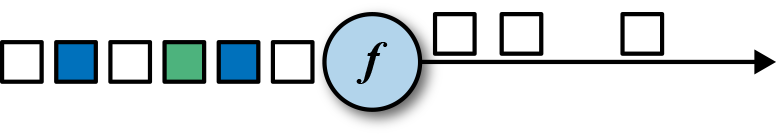
\includegraphics{images/spaf_0502.png}

布尔条件可以使用函数、FilterFunction接口或者匿名函数来实现。FilterFunction中的泛型是输入事件的类型。定义的filter()方法会作用在每一个输入元素上面,并返回一个布尔值。

\begin{Shaded}
\begin{Highlighting}[]
\CommentTok{// T: the type of elements}
\NormalTok{FilterFunction[T]}
\NormalTok{    \textgreater{} }\FunctionTok{filter}\NormalTok{(T): }\BuiltInTok{Boolean}
\end{Highlighting}
\end{Shaded}

下面的例子展示了如何使用filter来从传感器数据中过滤掉温度值小于25华氏温度的读数。

\begin{Shaded}
\begin{Highlighting}[]
\NormalTok{DataStream\textless{}SensorReading\textgreater{} filteredReadings = readings.}\FunctionTok{filter}\NormalTok{(r {-}\textgreater{} r.}\FunctionTok{temperature}\NormalTok{ \textgreater{}= }\DecValTok{25}\NormalTok{);}
\end{Highlighting}
\end{Shaded}

\emph{FLATMAP}

flatMap算子和map算子很类似,不同之处在于针对每一个输入事件flatMap可以生成0个、1个或者多个输出元素。事实上,flatMap转换算子是filter和map的泛化。所以flatMap可以实现map和filter算子的功能。图5-3展示了flatMap如何根据输入事件的颜色来做不同的处理。如果输入事件是白色方框,则直接输出。输入元素是黑框,则复制输入。灰色方框会被过滤掉。

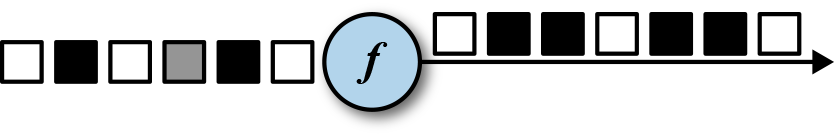
\includegraphics{images/spaf_0503.png}

flatMap算子将会应用在每一个输入事件上面。对应的FlatMapFunction定义了flatMap()方法,这个方法返回0个、1个或者多个事件到一个Collector集合中,作为输出结果。

\begin{Shaded}
\begin{Highlighting}[]
\CommentTok{// T: the type of input elements}
\CommentTok{// O: the type of output elements}
\NormalTok{FlatMapFunction[T, O]}
\NormalTok{    \textgreater{} }\FunctionTok{flatMap}\NormalTok{(T, Collector[O]): Unit}
\end{Highlighting}
\end{Shaded}

下面的例子展示了在数据分析教程中经常用到的例子,我们用flatMap来实现。使用\_来切割传感器ID,比如sensor\_1。

\begin{Shaded}
\begin{Highlighting}[]
\KeywordTok{public} \DataTypeTok{static} \KeywordTok{class}\NormalTok{ IdSplitter }\KeywordTok{implements}\NormalTok{ FlatMapFunction\textless{}}\BuiltInTok{String}\NormalTok{, }\BuiltInTok{String}\NormalTok{\textgreater{} \{}
    \AttributeTok{@Override}
    \KeywordTok{public} \DataTypeTok{void} \FunctionTok{flatMap}\NormalTok{(}\BuiltInTok{String}\NormalTok{ id, Collector\textless{}}\BuiltInTok{String}\NormalTok{\textgreater{} out) \{}

        \BuiltInTok{String}\NormalTok{[] splits = id.}\FunctionTok{split}\NormalTok{(}\StringTok{"\_"}\NormalTok{);}

        \KeywordTok{for}\NormalTok{ (}\BuiltInTok{String}\NormalTok{ split : splits) \{}
\NormalTok{            out.}\FunctionTok{collect}\NormalTok{(split);}
\NormalTok{        \}}
\NormalTok{    \}}
\NormalTok{\}}
\end{Highlighting}
\end{Shaded}

匿名函数写法:

\begin{Shaded}
\begin{Highlighting}[]
\NormalTok{DataStream\textless{}}\BuiltInTok{String}\NormalTok{\textgreater{} splitIds = sensorIds}
\NormalTok{    .}\FunctionTok{flatMap}\NormalTok{((FlatMapFunction\textless{}}\BuiltInTok{String}\NormalTok{, }\BuiltInTok{String}\NormalTok{\textgreater{})}
\NormalTok{            (id, out) {-}\textgreater{} \{ }\KeywordTok{for}\NormalTok{ (}\BuiltInTok{String}\NormalTok{ s: id.}\FunctionTok{split}\NormalTok{(}\StringTok{"\_"}\NormalTok{)) \{ out.}\FunctionTok{collect}\NormalTok{(s);\}\})}
    \CommentTok{// provide result type because Java cannot infer return type of lambda function}
    \CommentTok{// 提供结果的类型,因为Java无法推断匿名函数的返回值类型}
\NormalTok{    .}\FunctionTok{returns}\NormalTok{(}\BuiltInTok{Types}\NormalTok{.}\FunctionTok{STRING}\NormalTok{);}
\end{Highlighting}
\end{Shaded}

\hypertarget{ux952eux63a7ux6d41ux8f6cux6362ux7b97ux5b50}{%
\subsection{键控流转换算子}\label{ux952eux63a7ux6d41ux8f6cux6362ux7b97ux5b50}}

很多流处理程序的一个基本要求就是要能对数据进行分组,分组后的数据共享某一个相同的属性。DataStream
API提供了一个叫做KeyedStream的抽象,此抽象会从逻辑上对DataStream进行分区,分区后的数据拥有同样的Key值,分区后的流互不相关。

针对KeyedStream的状态转换操作可以读取数据或者写入数据到当前事件Key所对应的状态中。这表明拥有同样Key的所有事件都可以访问同样的状态,也就是说所以这些事件可以一起处理。

\begin{quote}
要小心使用状态转换操作和基于Key的聚合操作。如果Key的值越来越多,例如:Key是订单ID,我们必须及时清空Key所对应的状态,以免引起内存方面的问题。稍后我们会详细讲解。
\end{quote}

KeyedStream可以使用map,flatMap和filter算子来处理。接下来我们会使用keyBy算子来将DataStream转换成KeyedStream,并讲解基于key的转换操作:滚动聚合和reduce算子。

\emph{KEYBY}

keyBy通过指定key来将DataStream转换成KeyedStream。基于不同的key,流中的事件将被分配到不同的分区中去。所有具有相同key的事件将会在接下来的操作符的同一个子任务槽中进行处理。拥有不同key的事件可以在同一个任务中处理。但是算子只能访问当前事件的key所对应的状态。

如图5-4所示,把输入事件的颜色作为key,黑色的事件输出到了一个分区,其他颜色输出到了另一个分区。

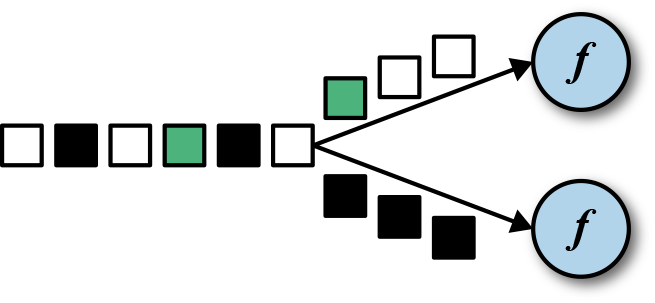
\includegraphics{images/spaf_0504.png}

keyBy()方法接收一个参数,这个参数指定了key或者keys,有很多不同的方法来指定key。我们将在后面讲解。下面的代码声明了id这个字段为SensorReading流的key。

\begin{Shaded}
\begin{Highlighting}[]
\NormalTok{KeyedStream\textless{}SensorReading, }\BuiltInTok{String}\NormalTok{\textgreater{} keyed = readings.}\FunctionTok{keyBy}\NormalTok{(r {-}\textgreater{} r.}\FunctionTok{id}\NormalTok{);}
\end{Highlighting}
\end{Shaded}

匿名函数r -\textgreater{} r.id抽取了传感器读数SensorReading的id值。

\emph{滚动聚合}

滚动聚合算子由KeyedStream调用,并生成一个聚合以后的DataStream,例如:sum,minimum,maximum。一个滚动聚合算子会为每一个观察到的key保存一个聚合的值。针对每一个输入事件,算子将会更新保存的聚合结果,并发送一个带有更新后的值的事件到下游算子。滚动聚合不需要用户自定义函数,但需要接受一个参数,这个参数指定了在哪一个字段上面做聚合操作。DataStream
API提供了以下滚动聚合方法。

\begin{quote}
滚动聚合算子只能用在滚动窗口,不能用在滑动窗口。
\end{quote}

\begin{itemize}
\tightlist
\item
  sum():在输入流上对指定的字段做滚动相加操作。
\item
  min():在输入流上对指定的字段求最小值。
\item
  max():在输入流上对指定的字段求最大值。
\item
  minBy():在输入流上针对指定字段求最小值,并返回包含当前观察到的最小值的事件。
\item
  maxBy():在输入流上针对指定字段求最大值,并返回包含当前观察到的最大值的事件。
\end{itemize}

滚动聚合算子无法组合起来使用,每次计算只能使用一个单独的滚动聚合算子。

下面的例子根据第一个字段来对类型为\texttt{Tuple3\textless{}Integer,\ Integer,\ Integer\textgreater{}}的流做分流操作,然后针对第二个字段做滚动求和操作。

\begin{Shaded}
\begin{Highlighting}[]
\NormalTok{DataStreamSource\textless{}Tuple3\textless{}}\BuiltInTok{Integer}\NormalTok{, }\BuiltInTok{Integer}\NormalTok{, }\BuiltInTok{Integer}\NormalTok{\textgreater{}\textgreater{} inputStream = env}
\NormalTok{    .}\FunctionTok{fromElements}\NormalTok{(}
\NormalTok{        Tuple3.}\FunctionTok{of}\NormalTok{(}\DecValTok{1}\NormalTok{, }\DecValTok{2}\NormalTok{, }\DecValTok{2}\NormalTok{),}
\NormalTok{        Tuple3.}\FunctionTok{of}\NormalTok{(}\DecValTok{2}\NormalTok{, }\DecValTok{3}\NormalTok{, }\DecValTok{1}\NormalTok{),}
\NormalTok{        Tuple3.}\FunctionTok{of}\NormalTok{(}\DecValTok{2}\NormalTok{, }\DecValTok{2}\NormalTok{, }\DecValTok{4}\NormalTok{),}
\NormalTok{        Tuple3.}\FunctionTok{of}\NormalTok{(}\DecValTok{1}\NormalTok{, }\DecValTok{5}\NormalTok{, }\DecValTok{3}\NormalTok{)}
\NormalTok{    );}

\NormalTok{DataStream\textless{}Tuple3\textless{}}\BuiltInTok{Integer}\NormalTok{, }\BuiltInTok{Integer}\NormalTok{, }\BuiltInTok{Integer}\NormalTok{\textgreater{}\textgreater{} resultStream = inputStream}
\NormalTok{  .}\FunctionTok{keyBy}\NormalTok{(}\DecValTok{0}\NormalTok{) }\CommentTok{// key on first field of the tuple}
\NormalTok{  .}\FunctionTok{sum}\NormalTok{(}\DecValTok{1}\NormalTok{);   }\CommentTok{// sum the second field of the tuple in place}
\end{Highlighting}
\end{Shaded}

在这个例子里面,输入流根据第一个字段来分流,然后在第二个字段上做计算。对于key
1,输出结果是(1,2,2),(1,7,2)。对于key
2,输出结果是(2,3,1),(2,5,1)。第一个字段是key,第二个字段是求和的数值,第三个字段未定义。

\begin{quote}
滚动聚合操作会对每一个key都保存一个状态。因为状态从来不会被清空,所以我们在使用滚动聚合算子时只能使用在含有有限个key的流上面。
\end{quote}

\emph{REDUCE}

reduce算子是滚动聚合的泛化实现。它将一个ReduceFunction应用到了一个KeyedStream上面去。reduce算子将会把每一个输入事件和当前已经reduce出来的值做聚合计算。reduce操作不会改变流的事件类型。输出流数据类型和输入流数据类型是一样的。

reduce函数可以通过实现接口ReduceFunction来创建一个类。ReduceFunction接口定义了reduce()方法,此方法接收两个输入事件,输出一个相同类型的事件。

\begin{Shaded}
\begin{Highlighting}[]
\CommentTok{// T: the element type}
\NormalTok{ReduceFunction[T]}
\NormalTok{    \textgreater{} }\FunctionTok{reduce}\NormalTok{(T, T): T}
\end{Highlighting}
\end{Shaded}

下面的例子,流根据传感器ID分流,然后计算每个传感器的当前最大温度值。

\begin{Shaded}
\begin{Highlighting}[]
\NormalTok{DataStream\textless{}SensorReading\textgreater{} maxTempPerSensor = keyed}
\NormalTok{        .}\FunctionTok{reduce}\NormalTok{((r1, r2) {-}\textgreater{} \{}
            \KeywordTok{if}\NormalTok{ (r1.}\FunctionTok{temperature}\NormalTok{ \textgreater{} r2.}\FunctionTok{temperature}\NormalTok{) \{}
                \KeywordTok{return}\NormalTok{ r1;}
\NormalTok{            \} }\KeywordTok{else}\NormalTok{ \{}
                \KeywordTok{return}\NormalTok{ r2;}
\NormalTok{            \}}
\NormalTok{        \});}
\end{Highlighting}
\end{Shaded}

\begin{quote}
reduce作为滚动聚合的泛化实现,同样也要针对每一个key保存状态。因为状态从来不会清空,所以我们需要将reduce算子应用在一个有限key的流上。
\end{quote}

\hypertarget{ux591aux6d41ux8f6cux6362ux7b97ux5b50}{%
\subsection{多流转换算子}\label{ux591aux6d41ux8f6cux6362ux7b97ux5b50}}

许多应用需要摄入多个流并将流合并处理,还可能需要将一条流分割成多条流然后针对每一条流应用不同的业务逻辑。接下来,我们将讨论DataStream
API中提供的能够处理多条输入流或者发送多条输出流的操作算子。

\emph{UNION}

DataStream.union()方法将两条或者多条DataStream合并成一条具有与输入流相同类型的输出DataStream。接下来的转换算子将会处理输入流中的所有元素。图5-5展示了union操作符如何将黑色和白色的事件流合并成一个单一输出流。

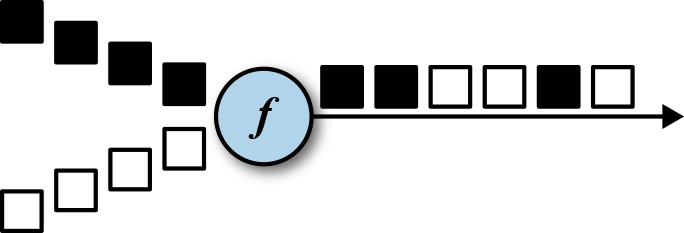
\includegraphics{images/spaf_0505.png}

事件合流的方式为FIFO方式。操作符并不会产生一个特定顺序的事件流。union操作符也不会进行去重。每一个输入事件都被发送到了下一个操作符。

下面的例子展示了如何将三条类型为SensorReading的数据流合并成一条流。

\begin{Shaded}
\begin{Highlighting}[]
\NormalTok{DataStream\textless{}SensorReading\textgreater{} parisStream = ...}
\NormalTok{DataStream\textless{}SensorReading\textgreater{} tokyoStream = ...}
\NormalTok{DataStream\textless{}SensorReading\textgreater{} rioStream = ...}
\NormalTok{DataStream\textless{}SensorReading\textgreater{} allCities = parisStream}
\NormalTok{  .}\FunctionTok{union}\NormalTok{(tokyoStream, rioStream);}
\end{Highlighting}
\end{Shaded}

\emph{CONNECT, COMAP和COFLATMAP}

联合两条流的事件是非常常见的流处理需求。例如监控一片森林然后发出高危的火警警报。报警的Application接收两条流,一条是温度传感器传回来的数据,一条是烟雾传感器传回来的数据。当两条流都超过各自的阈值时,报警。

DataStream
API提供了connect操作来支持以上的应用场景。DataStream.connect()方法接收一条DataStream,然后返回一个ConnectedStreams类型的对象,这个对象表示了两条连接的流。

\begin{Shaded}
\begin{Highlighting}[]
\CommentTok{// first stream}
\NormalTok{DataStream\textless{}}\BuiltInTok{Integer}\NormalTok{\textgreater{} first = ...}
\CommentTok{// second stream}
\NormalTok{DataStream\textless{}}\BuiltInTok{String}\NormalTok{\textgreater{} second = ...}

\CommentTok{// connect streams}
\NormalTok{ConnectedStreams\textless{}}\BuiltInTok{Integer}\NormalTok{, }\BuiltInTok{String}\NormalTok{\textgreater{} connected = first.}\FunctionTok{connect}\NormalTok{(second);}
\end{Highlighting}
\end{Shaded}

ConnectedStreams提供了map()和flatMap()方法,分别需要接收类型为CoMapFunction和CoFlatMapFunction的参数。

以上两个函数里面的泛型是第一条流的事件类型和第二条流的事件类型,以及输出流的事件类型。还定义了两个方法,每一个方法针对一条流来调用。map1()和flatMap1()会调用在第一条流的元素上面,map2()和flatMap2()会调用在第二条流的元素上面。

\begin{Shaded}
\begin{Highlighting}[]
\CommentTok{// IN1: 第一条流的事件类型}
\CommentTok{// IN2: 第二条流的事件类型}
\CommentTok{// OUT: 输出流的事件类型}
\NormalTok{CoMapFunction[IN1, IN2, OUT]}
\NormalTok{    \textgreater{} }\FunctionTok{map1}\NormalTok{(IN1): OUT}
\NormalTok{    \textgreater{} }\FunctionTok{map2}\NormalTok{(IN2): OUT}

\NormalTok{CoFlatMapFunction[IN1, IN2, OUT]}
\NormalTok{    \textgreater{} }\FunctionTok{flatMap1}\NormalTok{(IN1, Collector[OUT]): Unit}
\NormalTok{    \textgreater{} }\FunctionTok{flatMap2}\NormalTok{(IN2, Collector[OUT]): Unit}
\end{Highlighting}
\end{Shaded}

\begin{quote}
函数无法选择读某一条流。我们是无法控制函数中的两个方法的调用顺序的。当一条流中的元素到来时,将会调用相对应的方法。
\end{quote}

对两条流做连接查询通常需要这两条流基于某些条件被确定性的路由到操作符中相同的并行实例里面去。在默认情况下,connect()操作将不会对两条流的事件建立任何关系,所以两条流的事件将会随机的被发送到下游的算子实例里面去。这样的行为会产生不确定性的计算结果,显然不是我们想要的。为了针对ConnectedStreams进行确定性的转换操作,connect()方法可以和keyBy()或者broadcast()组合起来使用。我们首先看一下keyBy()的示例。

\begin{Shaded}
\begin{Highlighting}[]
\NormalTok{DataStream\textless{}Tuple2\textless{}}\BuiltInTok{Integer}\NormalTok{, }\BuiltInTok{Long}\NormalTok{\textgreater{}\textgreater{} one = ...}
\NormalTok{DataStream\textless{}Tuple2\textless{}}\BuiltInTok{Integer}\NormalTok{, }\BuiltInTok{String}\NormalTok{\textgreater{}\textgreater{} two = ...}

\CommentTok{// keyBy two connected streams}
\NormalTok{ConnectedStreams\textless{}Tuple2\textless{}}\BuiltInTok{Integer}\NormalTok{, }\BuiltInTok{Long}\NormalTok{\textgreater{}, Tuple2\textless{}}\BuiltInTok{Integer}\NormalTok{, }\BuiltInTok{String}\NormalTok{\textgreater{}\textgreater{} keyedConnect1 = one}
\NormalTok{  .}\FunctionTok{connect}\NormalTok{(two)}
\NormalTok{  .}\FunctionTok{keyBy}\NormalTok{(}\DecValTok{0}\NormalTok{, }\DecValTok{0}\NormalTok{); }\CommentTok{// key both input streams on first attribute}

\CommentTok{// alternative: connect two keyed streams}
\NormalTok{ConnectedStreams\textless{}Tuple2\textless{}}\BuiltInTok{Integer}\NormalTok{, }\BuiltInTok{Long}\NormalTok{\textgreater{}, Tuple2\textless{}}\BuiltInTok{Integer}\NormalTok{, }\BuiltInTok{String}\NormalTok{\textgreater{}\textgreater{} keyedConnect2 = one}
\NormalTok{  .}\FunctionTok{keyBy}\NormalTok{(}\DecValTok{0}\NormalTok{)}
\NormalTok{  .}\FunctionTok{connect}\NormalTok{(two.}\FunctionTok{keyBy}\NormalTok{(}\DecValTok{0}\NormalTok{));}
\end{Highlighting}
\end{Shaded}

无论使用keyBy()算子操作ConnectedStreams还是使用connect()算子连接两条KeyedStreams,connect()算子会将两条流的含有相同Key的所有事件都发送到相同的算子实例。两条流的key必须是一样的类型和值,就像SQL中的JOIN。在connected和keyed
stream上面执行的算子有访问keyed state的权限。

下面的例子展示了如何连接一条DataStream和广播过的流。

\begin{Shaded}
\begin{Highlighting}[]
\NormalTok{DataStream\textless{}Tuple2\textless{}}\BuiltInTok{Integer}\NormalTok{, }\BuiltInTok{Long}\NormalTok{\textgreater{}\textgreater{} one = ...}
\NormalTok{DataStream\textless{}Tuple2\textless{}}\BuiltInTok{Integer}\NormalTok{, }\BuiltInTok{String}\NormalTok{\textgreater{}\textgreater{} two = ...}

\CommentTok{// connect streams with broadcast}
\NormalTok{ConnectedStreams\textless{}Tuple2\textless{}}\BuiltInTok{Integer}\NormalTok{, }\BuiltInTok{Long}\NormalTok{\textgreater{}, Tuple2\textless{}}\BuiltInTok{Integer}\NormalTok{, }\BuiltInTok{String}\NormalTok{\textgreater{}\textgreater{} keyedConnect = first}
  \CommentTok{// broadcast second input stream}
\NormalTok{  .}\FunctionTok{connect}\NormalTok{(second.}\FunctionTok{broadcast}\NormalTok{());}
\end{Highlighting}
\end{Shaded}

一条被广播过的流中的所有元素将会被复制然后发送到下游算子的所有并行实例中去。未被广播过的流仅仅向前发送。所以两条流的元素显然会被连接处理。

\textbf{警告类}

\begin{Shaded}
\begin{Highlighting}[]
\KeywordTok{public} \KeywordTok{class}\NormalTok{ Alert \{}

    \KeywordTok{public} \BuiltInTok{String}\NormalTok{ message;}
    \KeywordTok{public} \DataTypeTok{long}\NormalTok{ timestamp;}

    \KeywordTok{public} \FunctionTok{Alert}\NormalTok{() \{ \}}

    \KeywordTok{public} \FunctionTok{Alert}\NormalTok{(}\BuiltInTok{String}\NormalTok{ message, }\DataTypeTok{long}\NormalTok{ timestamp) \{}
        \KeywordTok{this}\NormalTok{.}\FunctionTok{message}\NormalTok{ = message;}
        \KeywordTok{this}\NormalTok{.}\FunctionTok{timestamp}\NormalTok{ = timestamp;}
\NormalTok{    \}}

    \KeywordTok{public} \BuiltInTok{String} \FunctionTok{toString}\NormalTok{() \{}
        \KeywordTok{return} \StringTok{"("}\NormalTok{ + message + }\StringTok{", "}\NormalTok{ + timestamp + }\StringTok{")"}\NormalTok{;}
\NormalTok{    \}}
\NormalTok{\}}
\end{Highlighting}
\end{Shaded}

\textbf{烟雾传感器读数类}

\begin{Shaded}
\begin{Highlighting}[]
\KeywordTok{public} \KeywordTok{enum}\NormalTok{ SmokeLevel \{}
\NormalTok{    LOW,}
\NormalTok{    HIGH}
\NormalTok{\}}
\end{Highlighting}
\end{Shaded}

\textbf{产生烟雾传感器读数的自定义数据源}

\begin{Shaded}
\begin{Highlighting}[]
\KeywordTok{public} \KeywordTok{class}\NormalTok{ SmokeLevelSource }\KeywordTok{implements}\NormalTok{ SourceFunction\textless{}SmokeLevel\textgreater{} \{}

    \KeywordTok{private} \DataTypeTok{boolean}\NormalTok{ running = }\KeywordTok{true}\NormalTok{;}

    \AttributeTok{@Override}
    \KeywordTok{public} \DataTypeTok{void} \FunctionTok{run}\NormalTok{(SourceContext\textless{}SmokeLevel\textgreater{} srcCtx) }\KeywordTok{throws} \BuiltInTok{Exception}\NormalTok{ \{}

        \BuiltInTok{Random}\NormalTok{ rand = }\KeywordTok{new} \BuiltInTok{Random}\NormalTok{();}

        \KeywordTok{while}\NormalTok{ (running) \{}

            \KeywordTok{if}\NormalTok{ (rand.}\FunctionTok{nextGaussian}\NormalTok{() \textgreater{} }\FloatTok{0.}\DecValTok{8}\NormalTok{) \{}
\NormalTok{                srcCtx.}\FunctionTok{collect}\NormalTok{(SmokeLevel.}\FunctionTok{HIGH}\NormalTok{);}
\NormalTok{            \} }\KeywordTok{else}\NormalTok{ \{}
\NormalTok{                srcCtx.}\FunctionTok{collect}\NormalTok{(SmokeLevel.}\FunctionTok{LOW}\NormalTok{);}
\NormalTok{            \}}

            \BuiltInTok{Thread}\NormalTok{.}\FunctionTok{sleep}\NormalTok{(}\DecValTok{1000}\NormalTok{);}
\NormalTok{        \}}
\NormalTok{    \}}

    \AttributeTok{@Override}
    \KeywordTok{public} \DataTypeTok{void} \FunctionTok{cancel}\NormalTok{() \{}
        \KeywordTok{this}\NormalTok{.}\FunctionTok{running}\NormalTok{ = }\KeywordTok{false}\NormalTok{;}
\NormalTok{    \}}
\NormalTok{\}}
\end{Highlighting}
\end{Shaded}

监控一片森林然后发出高危的火警警报。报警的Application接收两条流,一条是温度传感器传回来的数据,一条是烟雾传感器传回来的数据。当两条流都超过各自的阈值时,报警。

\begin{Shaded}
\begin{Highlighting}[]
\KeywordTok{public} \KeywordTok{class}\NormalTok{ MultiStreamTransformations \{}

    \KeywordTok{public} \DataTypeTok{static} \DataTypeTok{void} \FunctionTok{main}\NormalTok{(}\BuiltInTok{String}\NormalTok{[] args) }\KeywordTok{throws} \BuiltInTok{Exception}\NormalTok{ \{}

\NormalTok{        StreamExecutionEnvironment env = StreamExecutionEnvironment.}\FunctionTok{getExecutionEnvironment}\NormalTok{();}

\NormalTok{        DataStream\textless{}SensorReading\textgreater{} tempReadings = env}
\NormalTok{                .}\FunctionTok{addSource}\NormalTok{(}\KeywordTok{new} \FunctionTok{SensorSource}\NormalTok{());}

\NormalTok{        DataStream\textless{}SmokeLevel\textgreater{} smokeReadings = env}
\NormalTok{                .}\FunctionTok{addSource}\NormalTok{(}\KeywordTok{new} \FunctionTok{SmokeLevelSource}\NormalTok{())}
\NormalTok{                .}\FunctionTok{setParallelism}\NormalTok{(}\DecValTok{1}\NormalTok{);}

\NormalTok{        KeyedStream\textless{}SensorReading, }\BuiltInTok{String}\NormalTok{\textgreater{} keyedTempReadings = tempReadings}
\NormalTok{                .}\FunctionTok{keyBy}\NormalTok{(r {-}\textgreater{} r.}\FunctionTok{id}\NormalTok{);}

\NormalTok{        DataStream\textless{}Alert\textgreater{} alerts = keyedTempReadings}
\NormalTok{                .}\FunctionTok{connect}\NormalTok{(smokeReadings.}\FunctionTok{broadcast}\NormalTok{())}
\NormalTok{                .}\FunctionTok{flatMap}\NormalTok{(}\KeywordTok{new} \FunctionTok{RaiseAlertFlatMap}\NormalTok{());}

\NormalTok{        alerts.}\FunctionTok{print}\NormalTok{();}

\NormalTok{        env.}\FunctionTok{execute}\NormalTok{(}\StringTok{"Multi{-}Stream Transformations Example"}\NormalTok{);}
\NormalTok{    \}}

    \KeywordTok{public} \DataTypeTok{static} \KeywordTok{class}\NormalTok{ RaiseAlertFlatMap }\KeywordTok{implements}\NormalTok{ CoFlatMapFunction\textless{}SensorReading, SmokeLevel, Alert\textgreater{} \{}

        \KeywordTok{private}\NormalTok{ SmokeLevel smokeLevel = SmokeLevel.}\FunctionTok{LOW}\NormalTok{;}

        \AttributeTok{@Override}
        \KeywordTok{public} \DataTypeTok{void} \FunctionTok{flatMap1}\NormalTok{(SensorReading tempReading, Collector\textless{}Alert\textgreater{} out) }\KeywordTok{throws} \BuiltInTok{Exception}\NormalTok{ \{}
            \CommentTok{// high chance of fire =\textgreater{} true}
            \KeywordTok{if}\NormalTok{ (}\KeywordTok{this}\NormalTok{.}\FunctionTok{smokeLevel}\NormalTok{ == SmokeLevel.}\FunctionTok{HIGH}\NormalTok{ \&\& tempReading.}\FunctionTok{temperature}\NormalTok{ \textgreater{} }\DecValTok{100}\NormalTok{) \{}
\NormalTok{                out.}\FunctionTok{collect}\NormalTok{(}\KeywordTok{new} \FunctionTok{Alert}\NormalTok{(}\StringTok{"Risk of fire! "}\NormalTok{ + tempReading, tempReading.}\FunctionTok{timestamp}\NormalTok{));}
\NormalTok{            \}}
\NormalTok{        \}}

        \AttributeTok{@Override}
        \KeywordTok{public} \DataTypeTok{void} \FunctionTok{flatMap2}\NormalTok{(SmokeLevel smokeLevel, Collector\textless{}Alert\textgreater{} out) \{}
            \CommentTok{// update smoke level}
            \KeywordTok{this}\NormalTok{.}\FunctionTok{smokeLevel}\NormalTok{ = smokeLevel;}
\NormalTok{        \}}
\NormalTok{    \}}
\NormalTok{\}}
\end{Highlighting}
\end{Shaded}

\hypertarget{ux5206ux5e03ux5f0fux8f6cux6362ux7b97ux5b50}{%
\subsection{分布式转换算子}\label{ux5206ux5e03ux5f0fux8f6cux6362ux7b97ux5b50}}

分区操作对应于我们之前讲过的``数据交换策略''这一节。这些操作定义了事件如何分配到不同的任务中去。当我们使用DataStream
API来编写程序时,系统将自动的选择数据分区策略,然后根据操作符的语义和设置的并行度将数据路由到正确的地方去。有些时候,我们需要在应用程序的层面控制分区策略,或者自定义分区策略。例如,如果我们知道会发生数据倾斜,那么我们想要针对数据流做负载均衡,将数据流平均发送到接下来的操作符中去。又或者,应用程序的业务逻辑可能需要一个算子所有的并行任务都需要接收同样的数据。再或者,我们需要自定义分区策略的时候。在这一小节,我们将展示DataStream的一些方法,可以使我们来控制或者自定义数据分区策略。

\begin{quote}
keyBy()方法不同于分布式转换算子。所有的分布式转换算子将产生DataStream数据类型。而keyBy()产生的类型是KeyedStream,它拥有自己的keyed
state。
\end{quote}

\emph{Random}

随机数据交换由DataStream.shuffle()方法实现。shuffle方法将数据随机的分配到下游算子的并行任务中去。

\emph{Round-Robin}

rebalance()方法使用Round-Robin负载均衡算法将输入流平均分配到随后的并行运行的任务中去。图5-7为round-robin分布式转换算子的示意图。

\emph{Rescale}

rescale()方法使用的也是round-robin算法,但只会将数据发送到接下来的并行运行的任务中的一部分任务中。本质上,当发送者任务数量和接收者任务数量不一样时,rescale分区策略提供了一种轻量级的负载均衡策略。如果接收者任务的数量是发送者任务的数量的倍数时,rescale操作将会效率更高。

rebalance()和rescale()的根本区别在于任务之间连接的机制不同。
rebalance()将会针对所有发送者任务和所有接收者任务之间建立通信通道,而rescale()仅仅针对每一个任务和下游算子的一部分子并行任务之间建立通信通道。rescale的示意图为图5-7。

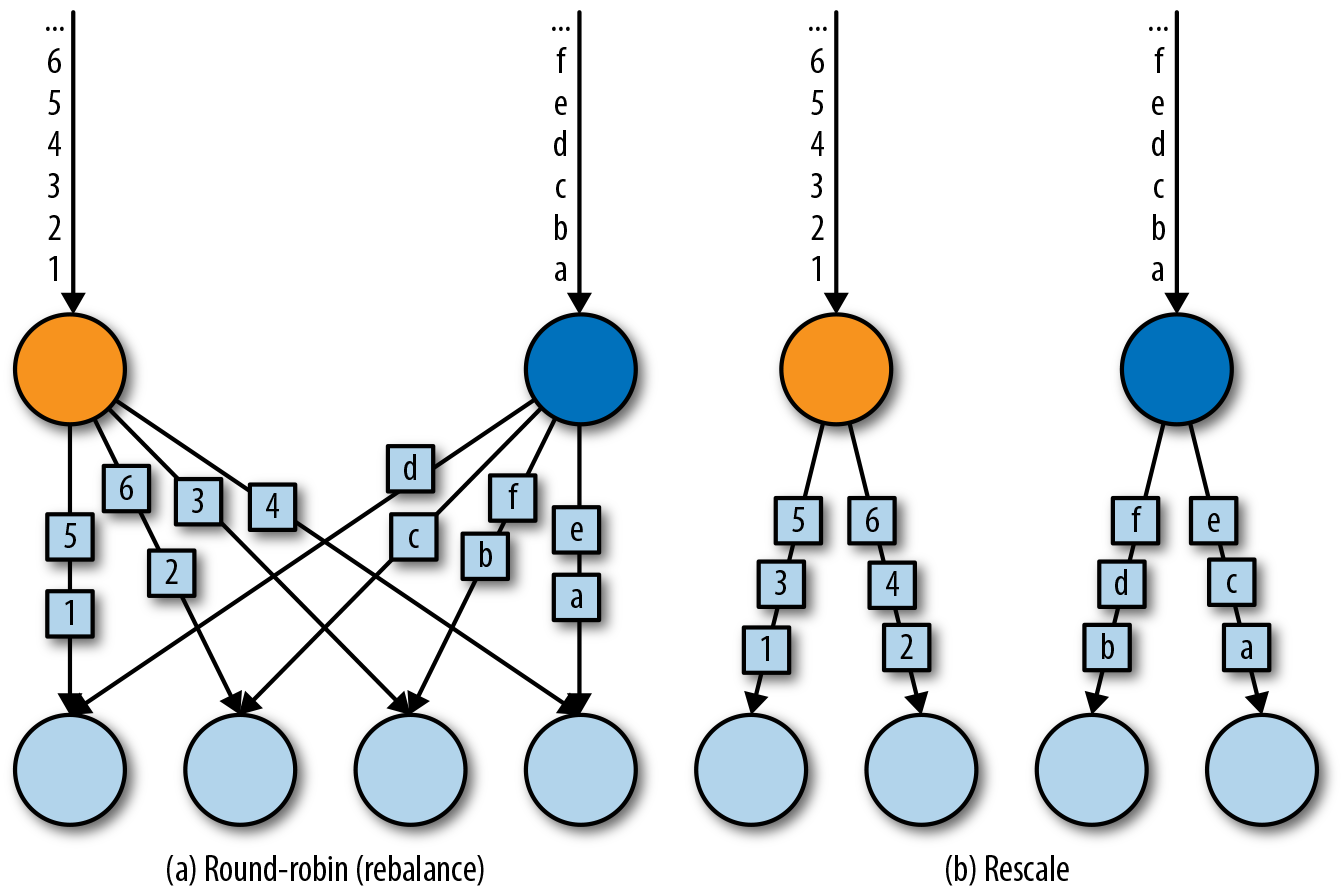
\includegraphics{images/spaf_0507.png}

\emph{Broadcast}

broadcast()方法将输入流的所有数据复制并发送到下游算子的所有并行任务中去。

\emph{Global}

global()方法将所有的输入流数据都发送到下游算子的第一个并行任务中去。这个操作需要很谨慎,因为将所有数据发送到同一个task,将会对应用程序造成很大的压力。

\emph{Custom}

当Flink提供的分区策略都不适用时,我们可以使用partitionCustom()方法来自定义分区策略。这个方法接收一个Partitioner对象,这个对象需要实现分区逻辑以及定义针对流的哪一个字段或者key来进行分区。

\hypertarget{ux8bbeux7f6eux5e76ux884cux5ea6}{%
\section{设置并行度}\label{ux8bbeux7f6eux5e76ux884cux5ea6}}

Flink应用程序在一个像集群这样的分布式环境中并行执行。当一个数据流程序提交到作业管理器执行时,系统将会创建一个数据流图,然后准备执行需要的操作符。每一个操作符将会并行化到一个或者多个任务中去。每个算子的并行任务都会处理这个算子的输入流中的一份子集。一个算子并行任务的个数叫做算子的并行度。它决定了算子执行的并行化程度,以及这个算子能处理多少数据量。

算子的并行度可以在执行环境这个层级来控制,也可以针对每个不同的算子设置不同的并行度。默认情况下,应用程序中所有算子的并行度都将设置为执行环境的并行度。执行环境的并行度(也就是所有算子的默认并行度)将在程序开始运行时自动初始化。如果应用程序在本地执行环境中运行,并行度将被设置为CPU的核数。当我们把应用程序提交到一个处于运行中的Flink集群时,执行环境的并行度将被设置为集群默认的并行度,除非我们在客户端提交应用程序时显式的设置好并行度。

通常情况下,将算子的并行度定义为和执行环境并行度相关的数值会是个好主意。这允许我们通过在客户端调整应用程序的并行度就可以将程序水平扩展了。我们可以使用以下代码来访问执行环境的默认并行度。

我们还可以重写执行环境的默认并行度,但这样的话我们将再也不能通过客户端来控制应用程序的并行度了。

算子默认的并行度也可以通过重写来明确指定。在下面的例子里面,数据源的操作符将会按照环境默认的并行度来并行执行,map操作符的并行度将会是默认并行度的2倍,sink操作符的并行度为2。

\begin{Shaded}
\begin{Highlighting}[]
\NormalTok{StreamExecutionEnvironment env = StreamExecutionEnvironment.}\FunctionTok{getExecutionEnvironment}\NormalTok{();}
\DataTypeTok{int}\NormalTok{ defaultP = env.}\FunctionTok{getParallelism}\NormalTok{();}
\NormalTok{env}
\NormalTok{  .}\FunctionTok{addSource}\NormalTok{(}\KeywordTok{new} \FunctionTok{CustomSource}\NormalTok{())}
\NormalTok{  .}\FunctionTok{map}\NormalTok{(}\KeywordTok{new} \FunctionTok{MyMapper}\NormalTok{())}
\NormalTok{  .}\FunctionTok{setParallelism}\NormalTok{(defaultP * }\DecValTok{2}\NormalTok{)}
\NormalTok{  .}\FunctionTok{print}\NormalTok{()}
\NormalTok{  .}\FunctionTok{setParallelism}\NormalTok{(}\DecValTok{2}\NormalTok{);}
\end{Highlighting}
\end{Shaded}

当我们通过客户端将应用程序的并行度设置为16并提交执行时,source操作符的并行度为16,mapper并行度为32,sink并行度为2。如果我们在本地环境运行应用程序的话,例如在IDE中运行,机器是8核,那么source任务将会并行执行在8个任务上面,mapper运行在16个任务上面,sink运行在2个任务上面。

\begin{quote}
并行度是动态概念,任务槽数量是静态概念。并行度\textless=任务槽数量。一个任务槽最多运行一个并行度。
\end{quote}

\hypertarget{ux7c7bux578b}{%
\section{类型}\label{ux7c7bux578b}}

Flink程序所处理的流中的事件一般是对象类型。操作符接收对象输出对象。所以Flink的内部机制需要能够处理事件的类型。在网络中传输数据,或者将数据写入到状态后端、检查点和保存点中,都需要我们对数据进行序列化和反序列化。为了高效的进行此类操作,Flink需要流中事件类型的详细信息。Flink使用了Type
Information的概念来表达数据类型,这样就能针对不同的数据类型产生特定的序列化器,反序列化器和比较操作符。

Flink也能够通过分析输入数据和输出数据来自动获取数据的类型信息以及序列化器和反序列化器。尽管如此,在一些特定的情况下,例如匿名函数或者使用泛型的情况下,我们需要明确的提供数据的类型信息,来提高我们程序的性能。

在这一节中,我们将讨论Flink支持的类型,以及如何为数据类型创建相应的类型信息,还有就是在Flink无法推断函数返回类型的情况下,如何帮助Flink的类型系统去做类型推断。

\hypertarget{ux652fux6301ux7684ux6570ux636eux7c7bux578b}{%
\subsection{支持的数据类型}\label{ux652fux6301ux7684ux6570ux636eux7c7bux578b}}

Flink支持Java提供的所有普通数据类型。最常用的数据类型可以做以下分类:

\begin{itemize}
\tightlist
\item
  Primitives(原始数据类型)
\item
  Flink专门为Java实现的Tuples(元组)
\item
  POJO类型
\item
  一些特殊的类型
\end{itemize}

接下来让我们一探究竟。

\emph{Primitives}

Java提供的所有原始数据类型都支持,例如Integer,String,Double等等。下面举一个例子:

\begin{Shaded}
\begin{Highlighting}[]
\NormalTok{DataStream\textless{}}\BuiltInTok{Long}\NormalTok{\textgreater{} numbers = env.}\FunctionTok{fromElements}\NormalTok{(}\DecValTok{1L}\NormalTok{, }\DecValTok{2L}\NormalTok{, }\DecValTok{3L}\NormalTok{, }\DecValTok{4L}\NormalTok{);}
\NormalTok{numbers.}\FunctionTok{map}\NormalTok{(n {-}\textgreater{} n + }\DecValTok{1}\NormalTok{);}
\end{Highlighting}
\end{Shaded}

\emph{Tuples}

元组是一种组合数据类型,由固定数量的元素组成。

Flink为Java的Tuple提供了高效的实现。Flink实现的Java
Tuple最多可以有25个元素,根据元素数量的不同,Tuple都被实现成了不同的类:Tuple1,Tuple2,一直到Tuple25。Tuple类是强类型。

\begin{Shaded}
\begin{Highlighting}[]
\NormalTok{DataStream\textless{}Tuple2\textless{}}\BuiltInTok{String}\NormalTok{, }\BuiltInTok{Integer}\NormalTok{\textgreater{}\textgreater{} persons = env}
\NormalTok{  .}\FunctionTok{fromElements}\NormalTok{(}
\NormalTok{    Tuple2.}\FunctionTok{of}\NormalTok{(}\StringTok{"Adam"}\NormalTok{, }\DecValTok{17}\NormalTok{),}
\NormalTok{    Tuple2.}\FunctionTok{of}\NormalTok{(}\StringTok{"Sarah"}\NormalTok{, }\DecValTok{23}\NormalTok{)}
\NormalTok{  );}

\NormalTok{persons.}\FunctionTok{filter}\NormalTok{(p {-}\textgreater{} p.}\FunctionTok{f1}\NormalTok{ \textgreater{} }\DecValTok{18}\NormalTok{);}
\end{Highlighting}
\end{Shaded}

Tuple的元素可以通过它们的public属性访问------f0,f1,f2等等。或者使用getField(int
pos)方法来访问,元素下标从0开始:

\begin{Shaded}
\begin{Highlighting}[]
\KeywordTok{import}\ImportTok{ org.apache.flink.api.java.tuple.Tuple2;}

\NormalTok{Tuple2\textless{}}\BuiltInTok{String}\NormalTok{, }\BuiltInTok{Integer}\NormalTok{\textgreater{} personTuple = Tuple2.}\FunctionTok{of}\NormalTok{(}\StringTok{"Alex"}\NormalTok{, }\DecValTok{42}\NormalTok{);}
\BuiltInTok{Integer}\NormalTok{ age = personTuple.}\FunctionTok{getField}\NormalTok{(}\DecValTok{1}\NormalTok{); }\CommentTok{// age = 42}
\end{Highlighting}
\end{Shaded}

Flink为Java实现的Tuple是可变数据结构,所以Tuple中的元素可以重新进行赋值。重复利用Java的Tuple可以减轻垃圾收集的压力。举个例子:

\begin{Shaded}
\begin{Highlighting}[]
\NormalTok{personTuple.}\FunctionTok{f1}\NormalTok{ = }\DecValTok{42}\NormalTok{; }\CommentTok{// set the 2nd field to 42}
\NormalTok{personTuple.}\FunctionTok{setField}\NormalTok{(}\DecValTok{43}\NormalTok{, }\DecValTok{1}\NormalTok{); }\CommentTok{// set the 2nd field to 43}
\end{Highlighting}
\end{Shaded}

\emph{POJO}

POJO类的定义:

\begin{itemize}
\tightlist
\item
  公有类
\item
  无参数的公有构造器
\item
  所有的字段都是公有的,可以通过getters和setters访问。
\item
  所有字段的数据类型都必须是Flink支持的数据类型。
\end{itemize}

举个例子:

\begin{Shaded}
\begin{Highlighting}[]
\KeywordTok{public} \KeywordTok{class}\NormalTok{ Person \{}
  \KeywordTok{public} \BuiltInTok{String}\NormalTok{ name;}
  \KeywordTok{public} \DataTypeTok{int}\NormalTok{ age;}

  \KeywordTok{public} \FunctionTok{Person}\NormalTok{() \{\}}

  \KeywordTok{public} \FunctionTok{Person}\NormalTok{(}\BuiltInTok{String}\NormalTok{ name, }\DataTypeTok{int}\NormalTok{ age) \{}
    \KeywordTok{this}\NormalTok{.}\FunctionTok{name}\NormalTok{ = name;}
    \KeywordTok{this}\NormalTok{.}\FunctionTok{age}\NormalTok{ = age;}
\NormalTok{  \}}
\NormalTok{\}}

\NormalTok{DataStream\textless{}Person\textgreater{} persons = env.}\FunctionTok{fromElements}\NormalTok{(}
  \KeywordTok{new} \FunctionTok{Person}\NormalTok{(}\StringTok{"Alex"}\NormalTok{, }\DecValTok{42}\NormalTok{),}
  \KeywordTok{new} \FunctionTok{Person}\NormalTok{(}\StringTok{"Wendy"}\NormalTok{, }\DecValTok{23}\NormalTok{)}
\NormalTok{);}
\end{Highlighting}
\end{Shaded}

\emph{其他数据类型}

\begin{itemize}
\tightlist
\item
  Array, ArrayList, HashMap, Enum
\item
  Hadoop Writable types
\end{itemize}

\hypertarget{ux4e3aux6570ux636eux7c7bux578bux521bux5efaux7c7bux578bux4fe1ux606f}{%
\subsection{为数据类型创建类型信息}\label{ux4e3aux6570ux636eux7c7bux578bux521bux5efaux7c7bux578bux4fe1ux606f}}

Flink类型系统的核心类是TypeInformation。它为系统在产生序列化器和比较操作符时,提供了必要的类型信息。例如,如果我们想使用某个key来做联结查询或者分组操作,TypeInformation可以让Flink做更严格的类型检查。

Flink针对Java提供了类来产生类型信息。在Java中,类是

\begin{Shaded}
\begin{Highlighting}[]
\NormalTok{org.}\FunctionTok{apache}\NormalTok{.}\FunctionTok{flink}\NormalTok{.}\FunctionTok{api}\NormalTok{.}\FunctionTok{common}\NormalTok{.}\FunctionTok{typeinfo}\NormalTok{.}\FunctionTok{Types}
\end{Highlighting}
\end{Shaded}

举个例子:

\begin{Shaded}
\begin{Highlighting}[]
\NormalTok{TypeInformation\textless{}}\BuiltInTok{Integer}\NormalTok{\textgreater{} intType = }\BuiltInTok{Types}\NormalTok{.}\FunctionTok{INT}\NormalTok{;}

\NormalTok{TypeInformation\textless{}Tuple2\textless{}}\BuiltInTok{Long}\NormalTok{, }\BuiltInTok{String}\NormalTok{\textgreater{}\textgreater{} tupleType = }\BuiltInTok{Types}
\NormalTok{  .}\FunctionTok{TUPLE}\NormalTok{(}\BuiltInTok{Types}\NormalTok{.}\FunctionTok{LONG}\NormalTok{, }\BuiltInTok{Types}\NormalTok{.}\FunctionTok{STRING}\NormalTok{);}

\NormalTok{TypeInformation\textless{}Person\textgreater{} personType = }\BuiltInTok{Types}
\NormalTok{  .}\FunctionTok{POJO}\NormalTok{(Person.}\FunctionTok{class}\NormalTok{);}
\end{Highlighting}
\end{Shaded}

\hypertarget{ux5bccux51fdux6570}{%
\section{富函数}\label{ux5bccux51fdux6570}}

我们经常会有这样的需求:在函数处理数据之前,需要做一些初始化的工作;或者需要在处理数据时可以获得函数执行上下文的一些信息;以及在处理完数据时做一些清理工作。而DataStream
API就提供了这样的机制。

DataStream
API提供的所有转换操作函数,都拥有它们的``富''版本,并且我们在使用常规函数或者匿名函数的地方来使用富函数。例如下面就是富函数的一些例子,可以看出,只需要在常规函数的前面加上Rich前缀就是富函数了。

\begin{itemize}
\tightlist
\item
  RichMapFunction
\item
  RichFlatMapFunction
\item
  RichFilterFunction
\item
  \ldots{}
\end{itemize}

当我们使用富函数时,我们可以实现两个额外的方法:

\begin{itemize}
\tightlist
\item
  open()方法是rich
  function的初始化方法,当一个算子例如map或者filter被调用之前open()会被调用。open()函数通常用来做一些只需要做一次即可的初始化工作。
\item
  close()方法是生命周期中的最后一个调用的方法,通常用来做一些清理工作。
\end{itemize}

另外,getRuntimeContext()方法提供了函数的RuntimeContext的一些信息,例如函数执行的并行度,当前子任务的索引,当前子任务的名字。同时还它还包含了访问分区状态的方法。下面看一个例子:

\begin{Shaded}
\begin{Highlighting}[]
\KeywordTok{public} \DataTypeTok{static} \KeywordTok{class}\NormalTok{ MyFlatMap }\KeywordTok{extends}\NormalTok{ RichFlatMapFunction\textless{}}\BuiltInTok{Integer}\NormalTok{, Tuple2\textless{}}\BuiltInTok{Integer}\NormalTok{, }\BuiltInTok{Integer}\NormalTok{\textgreater{}\textgreater{} \{}
  \KeywordTok{private} \DataTypeTok{int}\NormalTok{ subTaskIndex = }\DecValTok{0}\NormalTok{;}

  \AttributeTok{@Override}
  \KeywordTok{public} \DataTypeTok{void} \FunctionTok{open}\NormalTok{(}\BuiltInTok{Configuration}\NormalTok{ configuration) \{}
    \DataTypeTok{int}\NormalTok{ subTaskIndex = getRuntimeContext.}\FunctionTok{getIndexOfThisSubtask}\NormalTok{;}
    \CommentTok{// 做一些初始化工作}
    \CommentTok{// 例如建立一个和HDFS的连接}
\NormalTok{  \}}

  \AttributeTok{@Override}
  \KeywordTok{public} \DataTypeTok{void} \FunctionTok{flatMap}\NormalTok{(}\BuiltInTok{Integer}\NormalTok{ in, Collector\textless{}Tuple2\textless{}}\BuiltInTok{Integer}\NormalTok{, }\BuiltInTok{Integer}\NormalTok{\textgreater{}\textgreater{} out) \{}
    \KeywordTok{if}\NormalTok{ (in \% }\DecValTok{2}\NormalTok{ == subTaskIndex) \{}
\NormalTok{      out.}\FunctionTok{collect}\NormalTok{((subTaskIndex, in));}
\NormalTok{    \}}
\NormalTok{  \}}

  \AttributeTok{@Override}
  \KeywordTok{public} \DataTypeTok{void} \FunctionTok{close}\NormalTok{() \{}
    \CommentTok{// 清理工作,断开和HDFS的连接。}
\NormalTok{  \}}
\NormalTok{\}}
\end{Highlighting}
\end{Shaded}

\hypertarget{ux57faux4e8eux65f6ux95f4ux548cux7a97ux53e3ux7684ux64cdux4f5cux7b26}{%
\chapter{基于时间和窗口的操作符}\label{ux57faux4e8eux65f6ux95f4ux548cux7a97ux53e3ux7684ux64cdux4f5cux7b26}}

在本章,我们将要学习DataStream
API中处理时间和基于时间的操作符,例如窗口操作符。

首先,我们会学习如何定义时间属性,时间戳和水位线。然后我们将会学习底层操作process
function,它可以让我们访问时间戳和水位线,以及注册定时器事件。接下来,我们将会使用Flink的window
API,它提供了通常使用的各种窗口类型的内置实现。我们将会学到如何进行用户自定义窗口操作符,以及窗口的核心功能:assigners(分配器)、triggers(触发器)和evictors(清理器)。最后,我们将讨论如何基于时间来做流的联结查询,以及处理迟到事件的策略。

\hypertarget{ux8bbeux7f6eux65f6ux95f4ux5c5eux6027}{%
\section{设置时间属性}\label{ux8bbeux7f6eux65f6ux95f4ux5c5eux6027}}

如果我们想要在分布式流处理应用程序中定义有关时间的操作,彻底理解时间的语义是非常重要的。当我们指定了一个窗口去收集某1分钟内的数据时,这个长度为1分钟的桶中,到底应该包含哪些数据?

\emph{ProcessingTime}

\begin{quote}
机器时间在分布式系统中又叫做``墙上时钟''。
\end{quote}

当操作符执行时,此操作符看到的时间是操作符所在机器的机器时间。Processing-time
window的触发取决于机器时间,窗口包含的元素也是那个机器时间段内到达的元素。通常情况下,窗口操作符使用processing
time会导致不确定的结果,因为基于机器时间的窗口中收集的元素取决于元素到达的速度快慢。使用processing
time会为程序提供极低的延迟,因为无需等待水位线的到达。

\begin{quote}
如果要追求极限的低延迟,请使用ProcessingTime。
\end{quote}

\emph{EventTime}

当操作符执行时,操作符看的当前时间是由流中元素所携带的信息决定的。流中的每一个元素都必须包含时间戳信息。而系统的逻辑时钟由水位线(Watermark)定义。我们之前学习过,时间戳要么在事件进入流处理程序之前已经存在,要么就需要在程序的数据源(source)处进行分配。当水位线宣布特定时间段的数据都已经到达,事件时间窗口将会被触发计算。即使数据到达的顺序是乱序的,事件时间窗口的计算结果也将是确定性的。窗口的计算结果并不取决于元素到达的快与慢。

\begin{quote}
当水位线超过事件时间窗口的结束时间时,窗口将会闭合,不再接收数据,并触发计算。
\end{quote}

\emph{IngestionTime}

当事件进入source操作符时,source操作符所在机器的机器时间,就是此事件的``摄入时间''(IngestionTime),并同时产生水位线。IngestionTime相当于EventTime和ProcessingTime的混合体。一个事件的IngestionTime其实就是它进入流处理器中的时间。

\begin{quote}
IngestionTime没什么价值,既有EventTime的执行效率(比较低),有没有EventTime计算结果的准确性。
\end{quote}

Flink 1.12通过指定不同类型的窗口来使用不同的时间属性。

\hypertarget{ux5904ux7406ux65f6ux95f4ux8bbeux5b9a}{%
\subsection{处理时间设定}\label{ux5904ux7406ux65f6ux95f4ux8bbeux5b9a}}

我们写Flink程序一般遵循以下步骤:

\begin{itemize}
\tightlist
\item
  读取数据源
\item
  分流
\item
  开窗
\item
  聚合
\item
  输出结果
\end{itemize}

\emph{滚动窗口}

\begin{Shaded}
\begin{Highlighting}[]
\NormalTok{.}\FunctionTok{keyBy}\NormalTok{(...)}
\NormalTok{.}\FunctionTok{window}\NormalTok{(TumblingProcessingTimeWindows.}\FunctionTok{of}\NormalTok{(}\BuiltInTok{Time}\NormalTok{.}\FunctionTok{seconds}\NormalTok{(}\DecValTok{5}\NormalTok{)))}
\NormalTok{.}\FunctionTok{aggregate}\NormalTok{(...)}
\end{Highlighting}
\end{Shaded}

\emph{滑动窗口}

\begin{Shaded}
\begin{Highlighting}[]
\NormalTok{.}\FunctionTok{keyBy}\NormalTok{(...)}
\NormalTok{.}\FunctionTok{window}\NormalTok{(SlidingProcessingTimeWindows.}\FunctionTok{of}\NormalTok{(}\BuiltInTok{Time}\NormalTok{.}\FunctionTok{seconds}\NormalTok{(}\DecValTok{10}\NormalTok{), }\BuiltInTok{Time}\NormalTok{.}\FunctionTok{seconds}\NormalTok{(}\DecValTok{5}\NormalTok{)))}
\NormalTok{.}\FunctionTok{aggregate}\NormalTok{(...)}
\end{Highlighting}
\end{Shaded}

\emph{会话窗口}

\begin{Shaded}
\begin{Highlighting}[]
\NormalTok{.}\FunctionTok{keyBy}\NormalTok{(...)}
\NormalTok{.}\FunctionTok{window}\NormalTok{(ProcessingTimeSessionWindows.}\FunctionTok{withGap}\NormalTok{(}\BuiltInTok{Time}\NormalTok{.}\FunctionTok{seconds}\NormalTok{(}\DecValTok{10}\NormalTok{)))}
\NormalTok{.}\FunctionTok{aggregate}\NormalTok{(...)}
\end{Highlighting}
\end{Shaded}

\hypertarget{ux4e8bux4ef6ux65f6ux95f4ux8bbeux5b9aux548cux6c34ux4f4dux7ebfux7684ux4ea7ux751f}{%
\subsection{事件时间设定和水位线的产生}\label{ux4e8bux4ef6ux65f6ux95f4ux8bbeux5b9aux548cux6c34ux4f4dux7ebfux7684ux4ea7ux751f}}

\emph{滚动窗口}

\begin{Shaded}
\begin{Highlighting}[]
\NormalTok{.}\FunctionTok{keyBy}\NormalTok{(...)}
\NormalTok{.}\FunctionTok{window}\NormalTok{(TumblingEventTimeWindows.}\FunctionTok{of}\NormalTok{(}\BuiltInTok{Time}\NormalTok{.}\FunctionTok{seconds}\NormalTok{(}\DecValTok{5}\NormalTok{)))}
\NormalTok{.}\FunctionTok{aggregate}\NormalTok{(...)}
\end{Highlighting}
\end{Shaded}

\emph{滑动窗口}

\begin{Shaded}
\begin{Highlighting}[]
\NormalTok{.}\FunctionTok{keyBy}\NormalTok{(...)}
\NormalTok{.}\FunctionTok{window}\NormalTok{(SlidingEventTimeWindows.}\FunctionTok{of}\NormalTok{(}\BuiltInTok{Time}\NormalTok{.}\FunctionTok{seconds}\NormalTok{(}\DecValTok{10}\NormalTok{), }\BuiltInTok{Time}\NormalTok{.}\FunctionTok{seconds}\NormalTok{(}\DecValTok{5}\NormalTok{)))}
\NormalTok{.}\FunctionTok{aggregate}\NormalTok{(...)}
\end{Highlighting}
\end{Shaded}

\emph{会话窗口}

\begin{Shaded}
\begin{Highlighting}[]
\NormalTok{.}\FunctionTok{keyBy}\NormalTok{(...)}
\NormalTok{.}\FunctionTok{window}\NormalTok{(EventTimeSessionWindows.}\FunctionTok{withGap}\NormalTok{(}\BuiltInTok{Time}\NormalTok{.}\FunctionTok{seconds}\NormalTok{(}\DecValTok{10}\NormalTok{)))}
\NormalTok{.}\FunctionTok{aggregate}\NormalTok{(...)}
\end{Highlighting}
\end{Shaded}

如果使用事件时间,那么流中的事件必须包含这个事件真正发生的时间。使用了事件时间的流必须携带水位线。

时间戳和水位线的单位是毫秒,记时从1970-01-01T00:00:00Z开始。到达某个操作符的水位线就会告知这个操作符:小于等于水位线中携带的时间戳的事件都已经到达这个操作符了。时间戳和水位线可以由SourceFunction产生,或者由用户自定义的时间戳分配器和水位线产生器来生成。

Flink暴露了TimestampAssigner接口供我们实现,使我们可以自定义如何从事件数据中抽取时间戳。一般来说,时间戳分配器需要在source操作符后马上进行调用。

\begin{quote}
因为时间戳分配器看到的元素的顺序应该和source操作符产生数据的顺序是一样的,否则就乱了。这就是为什么我们经常将source操作符的并行度设置为1的原因。
\end{quote}

也就是说,任何分区操作都会将元素的顺序打乱,例如:并行度改变,keyBy()操作等等。

所以最佳实践是:在尽量接近数据源source操作符的地方分配时间戳和产生水位线,甚至最好在SourceFunction中分配时间戳和产生水位线。当然在分配时间戳和产生水位线之前可以对流进行map和filter操作是没问题的,也就是说必须是窄依赖。

以下这种写法是可以的。

\begin{Shaded}
\begin{Highlighting}[]
\NormalTok{DataStream\textless{}T\textgreater{} stream = env}
\NormalTok{  .}\FunctionTok{addSource}\NormalTok{(...)}
\NormalTok{  .}\FunctionTok{map}\NormalTok{(...)}
\NormalTok{  .}\FunctionTok{filter}\NormalTok{(...)}
\NormalTok{  .}\FunctionTok{assignTimestampsAndWatermarks}\NormalTok{(...)}
\end{Highlighting}
\end{Shaded}

我们来看一个例子,这个例子的最大延迟时间是5秒钟。

\begin{Shaded}
\begin{Highlighting}[]
\NormalTok{env}
\NormalTok{  .}\FunctionTok{addSource}\NormalTok{(}\KeywordTok{new} \FunctionTok{SensorSource}\NormalTok{())}
\NormalTok{  .}\FunctionTok{assignTimestampsAndWatermarks}\NormalTok{(}
\NormalTok{    WatermarkStrategy}
\NormalTok{      .\textless{}SensorReading\textgreater{}}\FunctionTok{forBoundedOutOfOrderness}\NormalTok{(}\BuiltInTok{Duration}\NormalTok{.}\FunctionTok{ofSeconds}\NormalTok{(}\DecValTok{5}\NormalTok{))}
\NormalTok{      .}\FunctionTok{withTimestampAssigner}\NormalTok{(}\KeywordTok{new}\NormalTok{ SerializableTimestampAssigner\textless{}SensorReading\textgreater{}() \{}
        \AttributeTok{@Override}
        \KeywordTok{public} \DataTypeTok{long} \FunctionTok{extractTimestamp}\NormalTok{(SensorReading element, }\DataTypeTok{long}\NormalTok{ recordTimestamp) \{}
          \KeywordTok{return}\NormalTok{ element.}\FunctionTok{timestamp}\NormalTok{;}
\NormalTok{        \}}
\NormalTok{      \}))}
\NormalTok{    .}\FunctionTok{keyBy}\NormalTok{(r {-}\textgreater{} r.}\FunctionTok{id}\NormalTok{)}
\NormalTok{    .}\FunctionTok{window}\NormalTok{(TumblingEventTimeWindows.}\FunctionTok{of}\NormalTok{(}\BuiltInTok{Time}\NormalTok{.}\FunctionTok{seconds}\NormalTok{(}\DecValTok{5}\NormalTok{)))}
\NormalTok{    .}\FunctionTok{aggregate}\NormalTok{(...)}
\end{Highlighting}
\end{Shaded}

如果我们已经知道到来的事件的时间戳是升序的,也就是最大延迟时间为0,那么我们可以使用如下写法:

\begin{Shaded}
\begin{Highlighting}[]
\NormalTok{env}
\NormalTok{  .}\FunctionTok{addSource}\NormalTok{(}\KeywordTok{new} \FunctionTok{SensorSource}\NormalTok{())}
\NormalTok{  .}\FunctionTok{assignTimestampsAndWatermarks}\NormalTok{(}
\NormalTok{    WatermarkStrategy.\textless{}SensorReading\textgreater{}}\FunctionTok{forMonotonousTimestamps}\NormalTok{()}
\NormalTok{      .}\FunctionTok{withTimestampAssigner}\NormalTok{(}\KeywordTok{new}\NormalTok{ SerializableTimestampAssigner\textless{}SensorReading\textgreater{}() \{}
        \AttributeTok{@Override}
        \KeywordTok{public} \DataTypeTok{long} \FunctionTok{extractTimestamp}\NormalTok{(SensorReading element, }\DataTypeTok{long}\NormalTok{ recordTimestamp) \{}
          \KeywordTok{return}\NormalTok{ element.}\FunctionTok{timestamp}\NormalTok{;}
\NormalTok{        \}}
\NormalTok{    \}))}
\NormalTok{    .}\FunctionTok{keyBy}\NormalTok{(r {-}\textgreater{} r.}\FunctionTok{id}\NormalTok{)}
\NormalTok{    .}\FunctionTok{window}\NormalTok{(TumblingEventTimeWindows.}\FunctionTok{of}\NormalTok{(}\BuiltInTok{Time}\NormalTok{.}\FunctionTok{seconds}\NormalTok{(}\DecValTok{5}\NormalTok{)))}
\NormalTok{    .}\FunctionTok{aggregate}\NormalTok{(...)}
\end{Highlighting}
\end{Shaded}

\hypertarget{ux81eaux5b9aux4e49ux6c34ux4f4dux7ebfux7684ux4ea7ux751fux903bux8f91}{%
\subsection{自定义水位线的产生逻辑}\label{ux81eaux5b9aux4e49ux6c34ux4f4dux7ebfux7684ux4ea7ux751fux903bux8f91}}

\textbf{产生水位线的接口}

\begin{Shaded}
\begin{Highlighting}[]
\AttributeTok{@Public}
\KeywordTok{public} \KeywordTok{interface}\NormalTok{ WatermarkGenerator\textless{}T\textgreater{} \{}

    \CommentTok{/**}
     \CommentTok{*}\NormalTok{ 每来一个事件都会调用}\CommentTok{,}\NormalTok{ 允许水位线产生器记忆和检查事件的时间戳。}
     \CommentTok{*}\NormalTok{ 允许水位线产生器基于事件本身发射水位线。}
     \CommentTok{*/}
    \DataTypeTok{void} \FunctionTok{onEvent}\NormalTok{(T event, }\DataTypeTok{long}\NormalTok{ eventTimestamp, WatermarkOutput output);}

    \CommentTok{/**}
     \CommentTok{*}\NormalTok{ 周期性的调用(默认}\CommentTok{200ms调用一次}\NormalTok{), 可能会产生新的水位线,也可能不会。}
     \CommentTok{*}
     \CommentTok{*}\NormalTok{ 调用周期通过ExecutionConfig}\CommentTok{\#}\NormalTok{getAutoWatermarkInterval}\CommentTok{()}\NormalTok{方法来配置。}
     \CommentTok{*/}
    \DataTypeTok{void} \FunctionTok{onPeriodicEmit}\NormalTok{(WatermarkOutput output);}
\NormalTok{\}}
\end{Highlighting}
\end{Shaded}

\textbf{周期性产生水位线}

\begin{Shaded}
\begin{Highlighting}[]
\KeywordTok{public} \KeywordTok{class}\NormalTok{ BoundedOutOfOrdernessGenerator }\KeywordTok{implements}\NormalTok{ WatermarkGenerator\textless{}MyEvent\textgreater{} \{}

    \KeywordTok{private} \DataTypeTok{final} \DataTypeTok{long}\NormalTok{ maxOutOfOrderness = }\DecValTok{3500}\NormalTok{; }\CommentTok{// 最大延迟时间是3.5s}

    \KeywordTok{private} \DataTypeTok{long}\NormalTok{ currentMaxTimestamp;}

    \AttributeTok{@Override}
    \KeywordTok{public} \DataTypeTok{void} \FunctionTok{onEvent}\NormalTok{(MyEvent event, }\DataTypeTok{long}\NormalTok{ eventTimestamp, WatermarkOutput output) \{}
\NormalTok{        currentMaxTimestamp = }\BuiltInTok{Math}\NormalTok{.}\FunctionTok{max}\NormalTok{(currentMaxTimestamp, eventTimestamp);}
\NormalTok{    \}}

    \AttributeTok{@Override}
    \KeywordTok{public} \DataTypeTok{void} \FunctionTok{onPeriodicEmit}\NormalTok{(WatermarkOutput output) \{}
        \CommentTok{// 产生水位线的公式:观察到的最大时间戳 {-} 最大延迟时间 {-} 1ms}
\NormalTok{        output.}\FunctionTok{emitWatermark}\NormalTok{(}\KeywordTok{new} \FunctionTok{Watermark}\NormalTok{(currentMaxTimestamp {-} maxOutOfOrderness {-} }\DecValTok{1}\NormalTok{));}
\NormalTok{    \}}

\NormalTok{\}}
\end{Highlighting}
\end{Shaded}

\textbf{不规则水位线的产生}

\begin{Shaded}
\begin{Highlighting}[]
\KeywordTok{public} \KeywordTok{class}\NormalTok{ PunctuatedAssigner }\KeywordTok{implements}\NormalTok{ WatermarkGenerator\textless{}MyEvent\textgreater{} \{}

    \AttributeTok{@Override}
    \KeywordTok{public} \DataTypeTok{void} \FunctionTok{onEvent}\NormalTok{(MyEvent event, }\DataTypeTok{long}\NormalTok{ eventTimestamp, WatermarkOutput output) \{}
        \KeywordTok{if}\NormalTok{ (event.}\FunctionTok{hasWatermarkMarker}\NormalTok{()) \{}
\NormalTok{            output.}\FunctionTok{emitWatermark}\NormalTok{(}\KeywordTok{new} \FunctionTok{Watermark}\NormalTok{(event.}\FunctionTok{getWatermarkTimestamp}\NormalTok{()));}
\NormalTok{        \}}
\NormalTok{    \}}

    \AttributeTok{@Override}
    \KeywordTok{public} \DataTypeTok{void} \FunctionTok{onPeriodicEmit}\NormalTok{(WatermarkOutput output) \{}
        \CommentTok{// 不需要做任何事情,因为我们在onEvent方法中发射了水位线}
\NormalTok{    \}}
\NormalTok{\}}
\end{Highlighting}
\end{Shaded}

\hypertarget{ux6c34ux4f4dux7ebfux603bux7ed3}{%
\subsection{水位线总结}\label{ux6c34ux4f4dux7ebfux603bux7ed3}}

\begin{quote}
水位线是一种逻辑时钟,Flink认为时间戳小于等于水位线的事件都到了。
\end{quote}

\begin{quote}
水位线 = 观察到的事件所包含的最大时间戳 - 最大延迟时间 - 1毫秒
\end{quote}

\begin{quote}
在事件时间的世界里,时间就是水位线。
\end{quote}

现在我们要讨论一下水位线会对我们的程序产生什么样的影响。

水位线用来平衡延迟和计算结果的正确性。水位线告诉我们,在触发计算(例如关闭窗口并触发窗口计算)之前,我们需要等待事件多长时间。基于事件时间的操作符根据水位线来衡量系统的逻辑时间的进度。

完美的水位线永远不会错:时间戳小于水位线的事件不会再出现。在特殊情况下(例如非乱序事件流),最近一次事件的时间戳就可能是完美的水位线。启发式水位线则相反,它只估计时间,因此有可能出错,即迟到的事件(其时间戳小于水位线标记时间)晚于水位线出现。针对启发式水位线,Flink提供了处理迟到元素的机制。

设定水位线通常需要用到领域知识。举例来说,如果知道事件的迟到时间不会超过5秒,就可以将水位线标记时间设为收到的最大时间戳减去5秒。另一种做法是,采用一个Flink作业监控事件流,学习事件的迟到规律,并以此构建水位线生成模型。

如果最大延迟时间设置的很大,计算出的结果会更精确,但收到计算结果的速度会很慢,同时系统会缓存大量的数据,并对系统造成比较大的压力。如果最大延迟时间设置的很小,那么收到计算结果的速度会很快,但可能收到错误的计算结果。不过Flink处理迟到数据的机制可以解决这个问题。上述问题看起来很复杂,但是恰恰符合现实世界的规律:大部分真实的事件流都是乱序的,并且通常无法了解它们的乱序程度(因为理论上不能预见未来)。水位线是唯一让我们直面乱序事件流并保证正确性的机制;
否则只能选择忽视事实,假装错误的结果是正确的。

\hypertarget{ux5904ux7406ux51fdux6570}{%
\section{处理函数}\label{ux5904ux7406ux51fdux6570}}

我们之前学习的转换算子是无法访问事件的时间戳信息和水位线信息的。而这在一些应用场景下,极为重要。例如MapFunction这样的map转换算子就无法访问时间戳或者当前事件的事件时间。

基于此,DataStream
API提供了一系列的Low-Level转换算子。可以访问时间戳、水位线以及注册定时事件。还可以输出特定的一些事件,例如超时事件等。Process
Function用来构建事件驱动的应用以及实现自定义的业务逻辑(使用之前的window函数和转换算子无法实现)。例如,Flink-SQL就是使用Process
Function实现的。

Flink提供了8个Process Function:

\begin{itemize}
\tightlist
\item
  ProcessFunction
\item
  KeyedProcessFunction
\item
  CoProcessFunction
\item
  ProcessJoinFunction
\item
  BroadcastProcessFunction
\item
  KeyedBroadcastProcessFunction
\item
  ProcessWindowFunction
\item
  ProcessAllWindowFunction
\end{itemize}

\hypertarget{keyedprocessfunctionux7684ux4f7fux7528}{%
\subsection{KeyedProcessFunction的使用}\label{keyedprocessfunctionux7684ux4f7fux7528}}

我们这里详细介绍一下KeyedProcessFunction。

KeyedProcessFunction用来操作KeyedStream。KeyedProcessFunction会处理流的每一个元素,输出为0个、1个或者多个元素。所有的Process
Function都继承自RichFunction接口,所以都有open()、close()和getRuntimeContext()等方法。而\texttt{KeyedProcessFunction\textless{}KEY,\ IN,\ OUT\textgreater{}}还额外提供了两个方法:

\begin{itemize}
\tightlist
\item
  \texttt{processElement(I\ value,\ Context\ ctx,\ Collector\textless{}O\textgreater{}\ out)}:流中的每一个元素都会调用这个方法,调用结果将会放在Collector数据类型中输出。Context可以访问元素的时间戳,元素的key,以及TimerService时间服务。Context还可以将结果输出到别的流(side
  outputs)。
\item
  \texttt{onTimer(long\ timestamp,\ OnTimerContext\ ctx,\ Collector\textless{}O\textgreater{}\ out)}:本方法是一个回调函数。当之前注册的定时器触发时调用。参数timestamp为定时器所设定的触发的时间戳。Collector为输出结果的集合。OnTimerContext和processElement的Context参数一样,提供了上下文的一些信息,例如firing
  trigger的时间信息(事件时间或者处理时间)。
\end{itemize}

\textbf{时间服务和定时器}

Context和OnTimerContext所持有的TimerService对象拥有以下方法:

\begin{itemize}
\tightlist
\item
  currentProcessingTime()返回当前处理时间
\item
  currentWatermark()返回当前水位线的时间戳
\item
  registerProcessingTimeTimer(long time)会注册当前key的processing
  time的timer。当processing time到达定时时间时,触发timer。
\item
  registerEventTimeTimer(long time)会注册当前key的event time
  timer。当水位线大于等于定时器注册的时间时,触发定时器执行回调函数。
\item
  deleteProcessingTimeTimer(long
  time)删除之前注册处理时间定时器。如果没有这个时间戳的定时器,则不执行。
\item
  deleteEventTimeTimer(long
  time)删除之前注册的事件时间定时器,如果没有此时间戳的定时器,则不执行。
\end{itemize}

当定时器timer触发时,执行回调函数onTimer()。processElement()方法和onTimer()方法是同步(不是异步)方法,这样可以避免并发访问和操作状态。

针对每一个key和timestamp,只能注册一个定期器。也就是说,每一个key可以注册多个定时器,但在每一个时间戳只能注册一个定时器。KeyedProcessFunction默认将所有定时器的时间戳放在一个优先队列中。在Flink做检查点操作时,定时器也会被保存到状态后端中。

举个例子说明KeyedProcessFunction如何操作KeyedStream。

下面的程序展示了如何监控温度传感器的温度值,如果温度值在一秒钟之内(processing
time)连续上升,报警。

主程序

\begin{Shaded}
\begin{Highlighting}[]
\NormalTok{DataStream\textless{}}\BuiltInTok{String}\NormalTok{\textgreater{} warings = readings}
\NormalTok{    .}\FunctionTok{keyBy}\NormalTok{(r {-}\textgreater{} r.}\FunctionTok{id}\NormalTok{)}
\NormalTok{    .}\FunctionTok{process}\NormalTok{(}\KeywordTok{new} \FunctionTok{TempIncreaseAlertFunction}\NormalTok{());}
\end{Highlighting}
\end{Shaded}

处理函数的实现如下

\begin{Shaded}
\begin{Highlighting}[]
\KeywordTok{public} \DataTypeTok{static} \KeywordTok{class}\NormalTok{ TempIncreaseAlertFunction }\KeywordTok{extends}\NormalTok{ KeyedProcessFunction\textless{}}\BuiltInTok{String}\NormalTok{, SensorReading, }\BuiltInTok{String}\NormalTok{\textgreater{} \{}

    \KeywordTok{private}\NormalTok{ ValueState\textless{}}\BuiltInTok{Double}\NormalTok{\textgreater{} lastTemp;}
    \KeywordTok{private}\NormalTok{ ValueState\textless{}}\BuiltInTok{Long}\NormalTok{\textgreater{} currentTimer;}

    \AttributeTok{@Override}
    \KeywordTok{public} \DataTypeTok{void} \FunctionTok{open}\NormalTok{(}\BuiltInTok{Configuration}\NormalTok{ parameters) }\KeywordTok{throws} \BuiltInTok{Exception}\NormalTok{ \{}
        \KeywordTok{super}\NormalTok{.}\FunctionTok{open}\NormalTok{(parameters);}
\NormalTok{        lastTemp = }\FunctionTok{getRuntimeContext}\NormalTok{().}\FunctionTok{getState}\NormalTok{(}
                \KeywordTok{new}\NormalTok{ ValueStateDescriptor\textless{}\textgreater{}(}\StringTok{"last{-}temp"}\NormalTok{, }\BuiltInTok{Types}\NormalTok{.}\FunctionTok{DOUBLE}\NormalTok{)}
\NormalTok{        );}
\NormalTok{        currentTimer = }\FunctionTok{getRuntimeContext}\NormalTok{().}\FunctionTok{getState}\NormalTok{(}
                \KeywordTok{new}\NormalTok{ ValueStateDescriptor\textless{}\textgreater{}(}\StringTok{"current{-}timer"}\NormalTok{, }\BuiltInTok{Types}\NormalTok{.}\FunctionTok{LONG}\NormalTok{)}
\NormalTok{        );}
\NormalTok{    \}}

    \AttributeTok{@Override}
    \KeywordTok{public} \DataTypeTok{void} \FunctionTok{processElement}\NormalTok{(SensorReading r, }\BuiltInTok{Context}\NormalTok{ ctx, Collector\textless{}}\BuiltInTok{String}\NormalTok{\textgreater{} out) }\KeywordTok{throws} \BuiltInTok{Exception}\NormalTok{ \{}
        \CommentTok{// 取出上一次的温度}
        \BuiltInTok{Double}\NormalTok{ prevTemp = }\FloatTok{0.}\DecValTok{0}\NormalTok{;}
        \KeywordTok{if}\NormalTok{ (lastTemp.}\FunctionTok{value}\NormalTok{() != }\KeywordTok{null}\NormalTok{) \{}
\NormalTok{            prevTemp = lastTemp.}\FunctionTok{value}\NormalTok{();}
\NormalTok{        \}}
        \CommentTok{// 将当前温度更新到上一次的温度这个变量中}
\NormalTok{        lastTemp.}\FunctionTok{update}\NormalTok{(r.}\FunctionTok{temperature}\NormalTok{);}

        \BuiltInTok{Long}\NormalTok{ curTimerTimestamp = }\DecValTok{0L}\NormalTok{;}
        \KeywordTok{if}\NormalTok{ (currentTimer.}\FunctionTok{value}\NormalTok{() != }\KeywordTok{null}\NormalTok{) \{}
\NormalTok{            curTimerTimestamp = currentTimer.}\FunctionTok{value}\NormalTok{();}
\NormalTok{        \}}
        \KeywordTok{if}\NormalTok{ (prevTemp == }\FloatTok{0.}\DecValTok{0}\NormalTok{ || r.}\FunctionTok{temperature}\NormalTok{ \textless{} prevTemp) \{}
            \CommentTok{// 温度下降或者是第一个温度值,删除定时器}
\NormalTok{            ctx.}\FunctionTok{timerService}\NormalTok{().}\FunctionTok{deleteProcessingTimeTimer}\NormalTok{(curTimerTimestamp);}
            \CommentTok{// 清空状态变量}
\NormalTok{            currentTimer.}\FunctionTok{clear}\NormalTok{();}
\NormalTok{        \} }\KeywordTok{else} \KeywordTok{if}\NormalTok{ (r.}\FunctionTok{temperature}\NormalTok{ \textgreater{} prevTemp \&\& curTimerTimestamp == }\DecValTok{0}\NormalTok{) \{}
            \CommentTok{// 温度上升且我们并没有设置定时器}
            \DataTypeTok{long}\NormalTok{ timerTs = ctx.}\FunctionTok{timerService}\NormalTok{().}\FunctionTok{currentProcessingTime}\NormalTok{() + }\DecValTok{1000L}\NormalTok{;}
\NormalTok{            ctx.}\FunctionTok{timerService}\NormalTok{().}\FunctionTok{registerProcessingTimeTimer}\NormalTok{(timerTs);}
            \CommentTok{// 保存定时器时间戳}
\NormalTok{            currentTimer.}\FunctionTok{update}\NormalTok{(timerTs);}
\NormalTok{        \}}
\NormalTok{    \}}

    \AttributeTok{@Override}
    \KeywordTok{public} \DataTypeTok{void} \FunctionTok{onTimer}\NormalTok{(}\DataTypeTok{long}\NormalTok{ timestamp, OnTimerContext ctx, Collector\textless{}}\BuiltInTok{String}\NormalTok{\textgreater{} out) }\KeywordTok{throws} \BuiltInTok{Exception}\NormalTok{ \{}
        \KeywordTok{super}\NormalTok{.}\FunctionTok{onTimer}\NormalTok{(timestamp, ctx, out);}
\NormalTok{        out.}\FunctionTok{collect}\NormalTok{(}\StringTok{"传感器id为: "}
\NormalTok{                + ctx.}\FunctionTok{getCurrentKey}\NormalTok{()}
\NormalTok{                + }\StringTok{"的传感器温度值已经连续1s上升了。"}\NormalTok{);}
\NormalTok{        currentTimer.}\FunctionTok{clear}\NormalTok{();}
\NormalTok{    \}}
\NormalTok{\}}
\end{Highlighting}
\end{Shaded}

\textbf{将事件发送到旁路输出}

大部分的DataStream
API的算子的输出是单一输出,也就是某种数据类型的流。除了split算子,可以将一条流分成多条流,这些流的数据类型也都相同。process
function的side
outputs功能可以产生多条流,并且这些流的数据类型可以不一样。一个side
output可以定义为\texttt{OutputTag\textless{}X\textgreater{}}对象,X是输出流的数据类型。process
function可以通过Context对象发射一个事件到一个或者多个side outputs。

\begin{Shaded}
\begin{Highlighting}[]
\KeywordTok{public} \KeywordTok{class}\NormalTok{ SideOutputExample \{}

    \KeywordTok{private} \DataTypeTok{static}\NormalTok{ OutputTag\textless{}}\BuiltInTok{String}\NormalTok{\textgreater{} output = }\KeywordTok{new}\NormalTok{ OutputTag\textless{}}\BuiltInTok{String}\NormalTok{\textgreater{}(}\StringTok{"side{-}output"}\NormalTok{)\{\};}

    \KeywordTok{public} \DataTypeTok{static} \DataTypeTok{void} \FunctionTok{main}\NormalTok{(}\BuiltInTok{String}\NormalTok{[] args) }\KeywordTok{throws} \BuiltInTok{Exception}\NormalTok{ \{}
\NormalTok{        StreamExecutionEnvironment env = StreamExecutionEnvironment.}\FunctionTok{getExecutionEnvironment}\NormalTok{();}
\NormalTok{        env.}\FunctionTok{setParallelism}\NormalTok{(}\DecValTok{1}\NormalTok{);}

\NormalTok{        DataStream\textless{}SensorReading\textgreater{} stream = env.}\FunctionTok{addSource}\NormalTok{(}\KeywordTok{new} \FunctionTok{SensorSource}\NormalTok{());}

\NormalTok{        SingleOutputStreamOperator\textless{}SensorReading\textgreater{} warnings = stream}
\NormalTok{                .}\FunctionTok{process}\NormalTok{(}\KeywordTok{new}\NormalTok{ ProcessFunction\textless{}SensorReading, SensorReading\textgreater{}() \{}
                    \AttributeTok{@Override}
                    \KeywordTok{public} \DataTypeTok{void} \FunctionTok{processElement}\NormalTok{(SensorReading value, }\BuiltInTok{Context}\NormalTok{ ctx, Collector\textless{}SensorReading\textgreater{} out) }\KeywordTok{throws} \BuiltInTok{Exception}\NormalTok{ \{}
                        \KeywordTok{if}\NormalTok{ (value.}\FunctionTok{temperature}\NormalTok{ \textless{} }\DecValTok{32}\NormalTok{) \{}
\NormalTok{                            ctx.}\FunctionTok{output}\NormalTok{(output, }\StringTok{"温度小于32度!"}\NormalTok{);}
\NormalTok{                        \}}
\NormalTok{                        out.}\FunctionTok{collect}\NormalTok{(value);}
\NormalTok{                    \}}
\NormalTok{                \});}

\NormalTok{        warnings.}\FunctionTok{print}\NormalTok{();}
\NormalTok{        warnings.}\FunctionTok{getSideOutput}\NormalTok{(output).}\FunctionTok{print}\NormalTok{();}

\NormalTok{        env.}\FunctionTok{execute}\NormalTok{();}
\NormalTok{    \}}
\NormalTok{\}}
\end{Highlighting}
\end{Shaded}

\hypertarget{coprocessfunctionux7684ux4f7fux7528}{%
\subsection{CoProcessFunction的使用}\label{coprocessfunctionux7684ux4f7fux7528}}

对于两条输入流,DataStream
API提供了CoProcessFunction这样的low-level操作。CoProcessFunction提供了操作每一个输入流的方法:
processElement1()和processElement2()。类似于ProcessFunction,这两种方法都通过Context对象来调用。这个Context对象可以访问事件数据,定时器时间戳,TimerService,以及side
outputs。CoProcessFunction也提供了onTimer()回调函数。下面的例子展示了如何使用CoProcessFunction来合并两条流。

\begin{Shaded}
\begin{Highlighting}[]
\KeywordTok{public} \KeywordTok{class}\NormalTok{ SensorSwitch \{}
    \KeywordTok{public} \DataTypeTok{static} \DataTypeTok{void} \FunctionTok{main}\NormalTok{(}\BuiltInTok{String}\NormalTok{[] args) }\KeywordTok{throws} \BuiltInTok{Exception}\NormalTok{ \{}
\NormalTok{        StreamExecutionEnvironment env = StreamExecutionEnvironment.}\FunctionTok{getExecutionEnvironment}\NormalTok{();}
\NormalTok{        env.}\FunctionTok{setParallelism}\NormalTok{(}\DecValTok{1}\NormalTok{);}

\NormalTok{        KeyedStream\textless{}SensorReading, }\BuiltInTok{String}\NormalTok{\textgreater{} stream = env}
\NormalTok{                .}\FunctionTok{addSource}\NormalTok{(}\KeywordTok{new} \FunctionTok{SensorSource}\NormalTok{())}
\NormalTok{                .}\FunctionTok{keyBy}\NormalTok{(r {-}\textgreater{} r.}\FunctionTok{id}\NormalTok{);}

\NormalTok{        KeyedStream\textless{}Tuple2\textless{}}\BuiltInTok{String}\NormalTok{, }\BuiltInTok{Long}\NormalTok{\textgreater{}, }\BuiltInTok{String}\NormalTok{\textgreater{} switches = env}
\NormalTok{                .}\FunctionTok{fromElements}\NormalTok{(Tuple2.}\FunctionTok{of}\NormalTok{(}\StringTok{"sensor\_2"}\NormalTok{, }\DecValTok{10}\NormalTok{ * }\DecValTok{1000L}\NormalTok{))}
\NormalTok{                .}\FunctionTok{keyBy}\NormalTok{(r {-}\textgreater{} r.}\FunctionTok{f0}\NormalTok{);}

\NormalTok{        stream}
\NormalTok{                .}\FunctionTok{connect}\NormalTok{(switches)}
\NormalTok{                .}\FunctionTok{process}\NormalTok{(}\KeywordTok{new} \FunctionTok{SwitchProcess}\NormalTok{())}
\NormalTok{                .}\FunctionTok{print}\NormalTok{();}

\NormalTok{        env.}\FunctionTok{execute}\NormalTok{();}
\NormalTok{    \}}

    \KeywordTok{public} \DataTypeTok{static} \KeywordTok{class}\NormalTok{ SwitchProcess }\KeywordTok{extends}\NormalTok{ CoProcessFunction\textless{}SensorReading, Tuple2\textless{}}\BuiltInTok{String}\NormalTok{, }\BuiltInTok{Long}\NormalTok{\textgreater{}, SensorReading\textgreater{} \{}

        \KeywordTok{private}\NormalTok{ ValueState\textless{}}\BuiltInTok{Boolean}\NormalTok{\textgreater{} forwardingEnabled;}

        \AttributeTok{@Override}
        \KeywordTok{public} \DataTypeTok{void} \FunctionTok{open}\NormalTok{(}\BuiltInTok{Configuration}\NormalTok{ parameters) }\KeywordTok{throws} \BuiltInTok{Exception}\NormalTok{ \{}
            \KeywordTok{super}\NormalTok{.}\FunctionTok{open}\NormalTok{(parameters);}
\NormalTok{            forwardingEnabled = }\FunctionTok{getRuntimeContext}\NormalTok{().}\FunctionTok{getState}\NormalTok{(}
                    \KeywordTok{new}\NormalTok{ ValueStateDescriptor\textless{}\textgreater{}(}\StringTok{"filterSwitch"}\NormalTok{, }\BuiltInTok{Types}\NormalTok{.}\FunctionTok{BOOLEAN}\NormalTok{)}
\NormalTok{            );}
\NormalTok{        \}}

        \AttributeTok{@Override}
        \KeywordTok{public} \DataTypeTok{void} \FunctionTok{processElement1}\NormalTok{(SensorReading value, }\BuiltInTok{Context}\NormalTok{ ctx, Collector\textless{}SensorReading\textgreater{} out) }\KeywordTok{throws} \BuiltInTok{Exception}\NormalTok{ \{}
            \KeywordTok{if}\NormalTok{ (forwardingEnabled.}\FunctionTok{value}\NormalTok{() != }\KeywordTok{null}\NormalTok{ \&\& forwardingEnabled.}\FunctionTok{value}\NormalTok{()) \{}
\NormalTok{                out.}\FunctionTok{collect}\NormalTok{(value);}
\NormalTok{            \}}
\NormalTok{        \}}

        \AttributeTok{@Override}
        \KeywordTok{public} \DataTypeTok{void} \FunctionTok{processElement2}\NormalTok{(Tuple2\textless{}}\BuiltInTok{String}\NormalTok{, }\BuiltInTok{Long}\NormalTok{\textgreater{} value, }\BuiltInTok{Context}\NormalTok{ ctx, Collector\textless{}SensorReading\textgreater{} out) }\KeywordTok{throws} \BuiltInTok{Exception}\NormalTok{ \{}
\NormalTok{            forwardingEnabled.}\FunctionTok{update}\NormalTok{(}\KeywordTok{true}\NormalTok{);}
\NormalTok{            ctx.}\FunctionTok{timerService}\NormalTok{().}\FunctionTok{registerProcessingTimeTimer}\NormalTok{(ctx.}\FunctionTok{timerService}\NormalTok{().}\FunctionTok{currentProcessingTime}\NormalTok{() + value.}\FunctionTok{f1}\NormalTok{);}
\NormalTok{        \}}

        \AttributeTok{@Override}
        \KeywordTok{public} \DataTypeTok{void} \FunctionTok{onTimer}\NormalTok{(}\DataTypeTok{long}\NormalTok{ timestamp, OnTimerContext ctx, Collector\textless{}SensorReading\textgreater{} out) }\KeywordTok{throws} \BuiltInTok{Exception}\NormalTok{ \{}
            \KeywordTok{super}\NormalTok{.}\FunctionTok{onTimer}\NormalTok{(timestamp, ctx, out);}
\NormalTok{            forwardingEnabled.}\FunctionTok{clear}\NormalTok{();}
\NormalTok{        \}}
\NormalTok{    \}}
\NormalTok{\}}
\end{Highlighting}
\end{Shaded}

\hypertarget{ux7a97ux53e3ux805aux5408ux51fdux6570ux7684ux4f7fux7528}{%
\subsection{窗口聚合函数的使用}\label{ux7a97ux53e3ux805aux5408ux51fdux6570ux7684ux4f7fux7528}}

窗口聚合函数定义了窗口中数据的计算逻辑。有两种计算逻辑:

\begin{itemize}
\tightlist
\item
  增量聚合函数:当一个事件被添加到窗口时,触发函数计算,并且更新window的状态(单个值)。最终聚合的结果将作为输出。ReduceFunction和AggregateFunction是增量聚合函数。
\item
  全窗口函数:这个函数将会收集窗口中所有的元素,可以做一些复杂计算。ProcessWindowFunction是全窗口聚合函数。
\end{itemize}

\textbf{增量聚合函数}

\begin{itemize}
\tightlist
\item
  每条数据到来就进行计算,只保存一个简单的状态(累加器)
\item
  ReduceFunction, AggregateFunction
\item
  当窗口闭合的时候,增量聚合完成
\item
  处理时间:当机器时间超过窗口结束时间的时候,窗口闭合
\item
  事件时间:当水位线超过窗口结束时间的时候,窗口闭合
\item
  来一条数据计算一次
\end{itemize}

\emph{REDUCE}

\begin{Shaded}
\begin{Highlighting}[]
\NormalTok{DataStream\textless{}Tuple2\textless{}}\BuiltInTok{String}\NormalTok{, }\BuiltInTok{Double}\NormalTok{\textgreater{}\textgreater{} minTempPerwindow = sensorData}
\NormalTok{    .}\FunctionTok{map}\NormalTok{(}\KeywordTok{new}\NormalTok{ MapFunction\textless{}SensorReading, Tuple2\textless{}}\BuiltInTok{String}\NormalTok{, }\BuiltInTok{Double}\NormalTok{\textgreater{}\textgreater{}() \{}
        \AttributeTok{@Override}
        \KeywordTok{public}\NormalTok{ Tuple2\textless{}}\BuiltInTok{String}\NormalTok{, }\BuiltInTok{Double}\NormalTok{\textgreater{} }\FunctionTok{map}\NormalTok{(SensorReading value) }\KeywordTok{throws} \BuiltInTok{Exception}\NormalTok{ \{}
            \KeywordTok{return}\NormalTok{ Tuple2.}\FunctionTok{of}\NormalTok{(value.}\FunctionTok{id}\NormalTok{, value.}\FunctionTok{temperature}\NormalTok{);}
\NormalTok{        \}}
\NormalTok{    \})}
\NormalTok{    .}\FunctionTok{keyBy}\NormalTok{(r {-}\textgreater{} r.}\FunctionTok{f0}\NormalTok{)}
\NormalTok{    .}\FunctionTok{window}\NormalTok{(TumblingProcessingTimeWindows.}\FunctionTok{of}\NormalTok{(}\BuiltInTok{Time}\NormalTok{.}\FunctionTok{seconds}\NormalTok{(}\DecValTok{5}\NormalTok{)))}
\NormalTok{    .}\FunctionTok{reduce}\NormalTok{(}\KeywordTok{new}\NormalTok{ ReduceFunction\textless{}Tuple2\textless{}}\BuiltInTok{String}\NormalTok{, }\BuiltInTok{Double}\NormalTok{\textgreater{}\textgreater{}() \{}
        \AttributeTok{@Override}
        \KeywordTok{public}\NormalTok{ Tuple2\textless{}}\BuiltInTok{String}\NormalTok{, }\BuiltInTok{Double}\NormalTok{\textgreater{} }\FunctionTok{reduce}\NormalTok{(Tuple2\textless{}}\BuiltInTok{String}\NormalTok{, }\BuiltInTok{Double}\NormalTok{\textgreater{} value1, Tuple2\textless{}}\BuiltInTok{String}\NormalTok{, }\BuiltInTok{Double}\NormalTok{\textgreater{} value2) }\KeywordTok{throws} \BuiltInTok{Exception}\NormalTok{ \{}
            \KeywordTok{if}\NormalTok{ (value1.}\FunctionTok{f1}\NormalTok{ \textless{} value2.}\FunctionTok{f1}\NormalTok{) \{}
                \KeywordTok{return}\NormalTok{ value1;}
\NormalTok{            \} }\KeywordTok{else}\NormalTok{ \{}
                \KeywordTok{return}\NormalTok{ value2;}
\NormalTok{            \}}
\NormalTok{        \}}
\NormalTok{    \})}
\end{Highlighting}
\end{Shaded}

\emph{AggregateFunction}

\includegraphics{images/spaf_0604.png}

先来看接口定义

\begin{Shaded}
\begin{Highlighting}[]
\KeywordTok{public} \KeywordTok{interface}\NormalTok{ AggregateFunction\textless{}IN, ACC, OUT\textgreater{} }\KeywordTok{extends}\NormalTok{ Function, }\BuiltInTok{Serializable}\NormalTok{ \{}

  \CommentTok{// 创建新累加器}
\NormalTok{  ACC }\FunctionTok{createAccumulator}\NormalTok{();}

  \CommentTok{// 累加操作的逻辑:将每一条输入元素累加到累加器上,并返回累加器}
\NormalTok{  ACC }\FunctionTok{add}\NormalTok{(IN value, ACC accumulator);}

  \CommentTok{// 返回累加结果}
\NormalTok{  OUT }\FunctionTok{getResult}\NormalTok{(ACC accumulator);}

  \CommentTok{// 将两个累加器聚合,只在事件时间会话窗口才会用到}
\NormalTok{  ACC }\FunctionTok{merge}\NormalTok{(ACC a, ACC b);}
\NormalTok{\}}
\end{Highlighting}
\end{Shaded}

IN是输入元素的类型,ACC是累加器的类型,OUT是输出元素的类型。

例子:计算窗口平均温度

\begin{Shaded}
\begin{Highlighting}[]
\NormalTok{stream}
\NormalTok{    .}\FunctionTok{keyBy}\NormalTok{(r {-}\textgreater{} r.}\FunctionTok{id}\NormalTok{)}
\NormalTok{    .}\FunctionTok{window}\NormalTok{(TumblingProcessingTimeWindows.}\FunctionTok{of}\NormalTok{(}\BuiltInTok{Time}\NormalTok{.}\FunctionTok{seconds}\NormalTok{(}\DecValTok{5}\NormalTok{)))}
\NormalTok{    .}\FunctionTok{aggregate}\NormalTok{(}\KeywordTok{new} \FunctionTok{AvgTemp}\NormalTok{())}
\NormalTok{    .}\FunctionTok{print}\NormalTok{();}

\KeywordTok{public} \DataTypeTok{static} \KeywordTok{class}\NormalTok{ AvgTemp }\KeywordTok{implements}\NormalTok{ AggregateFunction\textless{}SensorReading, Tuple3\textless{}}\BuiltInTok{String}\NormalTok{, }\BuiltInTok{Double}\NormalTok{, }\BuiltInTok{Long}\NormalTok{\textgreater{}, Tuple2\textless{}}\BuiltInTok{String}\NormalTok{, }\BuiltInTok{Double}\NormalTok{\textgreater{}\textgreater{} \{}
    \AttributeTok{@Override}
    \KeywordTok{public}\NormalTok{ Tuple3\textless{}}\BuiltInTok{String}\NormalTok{, }\BuiltInTok{Double}\NormalTok{, }\BuiltInTok{Long}\NormalTok{\textgreater{} }\FunctionTok{createAccumulator}\NormalTok{() \{}
        \KeywordTok{return}\NormalTok{ Tuple3.}\FunctionTok{of}\NormalTok{(}\StringTok{""}\NormalTok{, }\FloatTok{0.}\DecValTok{0}\NormalTok{, }\DecValTok{0L}\NormalTok{);}
\NormalTok{    \}}

    \AttributeTok{@Override}
    \KeywordTok{public}\NormalTok{ Tuple3\textless{}}\BuiltInTok{String}\NormalTok{, }\BuiltInTok{Double}\NormalTok{, }\BuiltInTok{Long}\NormalTok{\textgreater{} }\FunctionTok{add}\NormalTok{(SensorReading value, Tuple3\textless{}}\BuiltInTok{String}\NormalTok{, }\BuiltInTok{Double}\NormalTok{, }\BuiltInTok{Long}\NormalTok{\textgreater{} accumulator) \{}
        \KeywordTok{return}\NormalTok{ Tuple3.}\FunctionTok{of}\NormalTok{(value.}\FunctionTok{id}\NormalTok{, accumulator.}\FunctionTok{f1}\NormalTok{ + value.}\FunctionTok{temperature}\NormalTok{, accumulator.}\FunctionTok{f2}\NormalTok{ + }\DecValTok{1}\NormalTok{);}
\NormalTok{    \}}

    \AttributeTok{@Override}
    \KeywordTok{public}\NormalTok{ Tuple2\textless{}}\BuiltInTok{String}\NormalTok{, }\BuiltInTok{Double}\NormalTok{\textgreater{} }\FunctionTok{getResult}\NormalTok{(Tuple3\textless{}}\BuiltInTok{String}\NormalTok{, }\BuiltInTok{Double}\NormalTok{, }\BuiltInTok{Long}\NormalTok{\textgreater{} accumulator) \{}
        \KeywordTok{return}\NormalTok{ Tuple2.}\FunctionTok{of}\NormalTok{(accumulator.}\FunctionTok{f0}\NormalTok{, accumulator.}\FunctionTok{f1}\NormalTok{ / accumulator.}\FunctionTok{f2}\NormalTok{);}
\NormalTok{    \}}

    \AttributeTok{@Override}
    \KeywordTok{public}\NormalTok{ Tuple3\textless{}}\BuiltInTok{String}\NormalTok{, }\BuiltInTok{Double}\NormalTok{, }\BuiltInTok{Long}\NormalTok{\textgreater{} }\FunctionTok{merge}\NormalTok{(Tuple3\textless{}}\BuiltInTok{String}\NormalTok{, }\BuiltInTok{Double}\NormalTok{, }\BuiltInTok{Long}\NormalTok{\textgreater{} a, Tuple3\textless{}}\BuiltInTok{String}\NormalTok{, }\BuiltInTok{Double}\NormalTok{, }\BuiltInTok{Long}\NormalTok{\textgreater{} b) \{}
        \KeywordTok{return} \KeywordTok{null}\NormalTok{;}
\NormalTok{    \}}
\NormalTok{\}}
\end{Highlighting}
\end{Shaded}

\textbf{全窗口聚合函数}

\includegraphics{images/spaf_0605.png}

一些业务场景,我们需要收集窗口内所有的数据进行计算,例如计算窗口数据的中位数,或者计算窗口数据中出现频率最高的值。这样的需求,使用ReduceFunction和AggregateFunction就无法实现了。这个时候就需要ProcessWindowFunction了。

先来看接口定义

\begin{Shaded}
\begin{Highlighting}[]
\KeywordTok{public} \KeywordTok{abstract} \KeywordTok{class}\NormalTok{ ProcessWindowFunction\textless{}IN, OUT, KEY, W }\KeywordTok{extends} \BuiltInTok{Window}\NormalTok{\textgreater{} }\KeywordTok{extends}\NormalTok{ AbstractRichFunction \{}

  \CommentTok{// 对窗口进行求值}
  \DataTypeTok{void} \FunctionTok{process}\NormalTok{(KEY key, }\BuiltInTok{Context}\NormalTok{ ctx, }\BuiltInTok{Iterable}\NormalTok{\textless{}IN\textgreater{} vals, Collector\textless{}OUT\textgreater{} out)}
    \KeywordTok{throws} \BuiltInTok{Exception}\NormalTok{;}

  \CommentTok{// Deletes any custom per{-}window state when the window is purged}
  \KeywordTok{public} \DataTypeTok{void} \FunctionTok{clear}\NormalTok{(}\BuiltInTok{Context}\NormalTok{ ctx) }\KeywordTok{throws} \BuiltInTok{Exception}\NormalTok{ \{\}}

  \CommentTok{// 持有窗口元数据的上下文}
  \KeywordTok{public} \KeywordTok{abstract} \KeywordTok{class} \BuiltInTok{Context} \KeywordTok{implements} \BuiltInTok{Serializable}\NormalTok{ \{}
    \CommentTok{// Returns the metadata of the window}
    \KeywordTok{public} \KeywordTok{abstract}\NormalTok{ W }\FunctionTok{window}\NormalTok{();}

    \CommentTok{// 返回当前处理时间}
    \KeywordTok{public} \KeywordTok{abstract} \DataTypeTok{long} \FunctionTok{currentProcessingTime}\NormalTok{();}

    \CommentTok{// 返回当前水位线}
    \KeywordTok{public} \KeywordTok{abstract} \DataTypeTok{long} \FunctionTok{currentWatermark}\NormalTok{();}

    \CommentTok{// State accessor for per{-}window state}
    \KeywordTok{public} \KeywordTok{abstract}\NormalTok{ KeyedStateStore }\FunctionTok{windowState}\NormalTok{();}

    \CommentTok{// State accessor for per{-}key global state}
    \KeywordTok{public} \KeywordTok{abstract}\NormalTok{ KeyedStateStore }\FunctionTok{globalState}\NormalTok{();}

    \CommentTok{// Emits a record to the side output identified by the OutputTag.}
    \KeywordTok{public} \KeywordTok{abstract}\NormalTok{ \textless{}X\textgreater{} }\DataTypeTok{void} \FunctionTok{output}\NormalTok{(OutputTag\textless{}X\textgreater{} outputTag, X value);}
\NormalTok{  \}}
\NormalTok{\}}
\end{Highlighting}
\end{Shaded}

process()方法接受的参数为:window的key,Iterable迭代器包含窗口的所有元素,Collector用于输出结果流。Context参数和别的process方法一样。而ProcessWindowFunction的Context对象还可以访问window的元数据(窗口开始和结束时间),当前处理时间和水位线,per-window
state和per-key global state,side outputs。

\begin{itemize}
\tightlist
\item
  per-window state:
  用于保存一些信息,这些信息可以被process()访问,只要process所处理的元素属于这个窗口。
\item
  per-key global state:
  同一个key,也就是在一条KeyedStream上,不同的window可以访问per-key
  global state保存的值。
\end{itemize}

例子:计算5s滚动窗口中的最低和最高的温度。输出的元素包含了(流的Key,
最低温度, 最高温度, 窗口结束时间)。

\begin{Shaded}
\begin{Highlighting}[]
\NormalTok{stream}
\NormalTok{    .}\FunctionTok{keyBy}\NormalTok{(r {-}\textgreater{} r.}\FunctionTok{id}\NormalTok{)}
\NormalTok{    .}\FunctionTok{window}\NormalTok{(TumblingProcessingTimeWindows.}\FunctionTok{of}\NormalTok{(}\BuiltInTok{Time}\NormalTok{.}\FunctionTok{seconds}\NormalTok{(}\DecValTok{5}\NormalTok{)))}
\NormalTok{    .}\FunctionTok{process}\NormalTok{(}\KeywordTok{new}\NormalTok{ ProcessWindowFunction\textless{}SensorReading, MinMaxTemp, }\BuiltInTok{String}\NormalTok{, TimeWindow\textgreater{}() \{}
        \AttributeTok{@Override}
        \KeywordTok{public} \DataTypeTok{void} \FunctionTok{process}\NormalTok{(}\BuiltInTok{String}\NormalTok{ s, }\BuiltInTok{Context}\NormalTok{ context, }\BuiltInTok{Iterable}\NormalTok{\textless{}SensorReading\textgreater{} elements, Collector\textless{}MinMaxTemp\textgreater{} out) }\KeywordTok{throws} \BuiltInTok{Exception}\NormalTok{ \{}
            \DataTypeTok{double}\NormalTok{ min = }\BuiltInTok{Double}\NormalTok{.}\FunctionTok{MAX\_VALUE}\NormalTok{;}
            \DataTypeTok{double}\NormalTok{ max = }\BuiltInTok{Double}\NormalTok{.}\FunctionTok{MIN\_VALUE}\NormalTok{;}
            \KeywordTok{for}\NormalTok{ (SensorReading element : elements) \{}
                \DataTypeTok{double}\NormalTok{ temp = element.}\FunctionTok{temperature}\NormalTok{;}
                \KeywordTok{if}\NormalTok{ (temp \textgreater{}= max) \{}
\NormalTok{                    max = temp;}
\NormalTok{                \}}
                \KeywordTok{if}\NormalTok{ (temp \textless{} min) \{}
\NormalTok{                    min = temp;}
\NormalTok{                \}}
\NormalTok{            \}}
\NormalTok{            out.}\FunctionTok{collect}\NormalTok{(}\KeywordTok{new} \FunctionTok{MinMaxTemp}\NormalTok{(s, min, max, ((}\BuiltInTok{Long}\NormalTok{)context.}\FunctionTok{window}\NormalTok{().}\FunctionTok{getEnd}\NormalTok{()).}\FunctionTok{toString}\NormalTok{()));}
\NormalTok{        \}}
\NormalTok{    \})}
\NormalTok{    .}\FunctionTok{print}\NormalTok{();}
\end{Highlighting}
\end{Shaded}

\textbf{增量聚合和全窗口聚合结合使用}

\includegraphics{images/spaf_0606.png}

我们还可以将ReduceFunction/AggregateFunction和ProcessWindowFunction结合起来使用。ReduceFunction/AggregateFunction做增量聚合,ProcessWindowFunction提供更多的对数据流的访问权限。如果只使用ProcessWindowFunction(底层的实现为将事件都保存在ListState中),将会非常占用空间。分配到某个窗口的元素将被提前聚合,而当窗口的trigger触发时,也就是窗口收集完数据关闭时,将会把聚合结果发送到ProcessWindowFunction中,这时Iterable参数将会只有一个值,就是前面聚合的值。

我们把前面的例子用这种方式重新写一下

\begin{Shaded}
\begin{Highlighting}[]
\NormalTok{stream}
\NormalTok{    .}\FunctionTok{keyBy}\NormalTok{(r {-}\textgreater{} r.}\FunctionTok{id}\NormalTok{)}
\NormalTok{    .}\FunctionTok{window}\NormalTok{(TumblingProcessingTimeWindows.}\FunctionTok{of}\NormalTok{(}\BuiltInTok{Time}\NormalTok{.}\FunctionTok{seconds}\NormalTok{(}\DecValTok{5}\NormalTok{)))}
\NormalTok{    .}\FunctionTok{aggregate}\NormalTok{(}\KeywordTok{new} \FunctionTok{Agg}\NormalTok{(), }\KeywordTok{new} \FunctionTok{Win}\NormalTok{())}
\NormalTok{    .}\FunctionTok{print}\NormalTok{();}

\KeywordTok{public} \DataTypeTok{static} \KeywordTok{class}\NormalTok{ Win }\KeywordTok{extends}\NormalTok{ ProcessWindowFunction\textless{}Tuple2\textless{}}\BuiltInTok{Double}\NormalTok{, }\BuiltInTok{Double}\NormalTok{\textgreater{}, MinMaxTemp, }\BuiltInTok{String}\NormalTok{, TimeWindow\textgreater{} \{}
    \AttributeTok{@Override}
    \KeywordTok{public} \DataTypeTok{void} \FunctionTok{process}\NormalTok{(}\BuiltInTok{String}\NormalTok{ s, }\BuiltInTok{Context}\NormalTok{ context, }\BuiltInTok{Iterable}\NormalTok{\textless{}Tuple2\textless{}}\BuiltInTok{Double}\NormalTok{, }\BuiltInTok{Double}\NormalTok{\textgreater{}\textgreater{} elements, Collector\textless{}MinMaxTemp\textgreater{} out) }\KeywordTok{throws} \BuiltInTok{Exception}\NormalTok{ \{}
\NormalTok{        Tuple2\textless{}}\BuiltInTok{Double}\NormalTok{, }\BuiltInTok{Double}\NormalTok{\textgreater{} minMax = elements.}\FunctionTok{iterator}\NormalTok{().}\FunctionTok{next}\NormalTok{();}
\NormalTok{        out.}\FunctionTok{collect}\NormalTok{(}\KeywordTok{new} \FunctionTok{MinMaxTemp}\NormalTok{(s, minMax.}\FunctionTok{f0}\NormalTok{, minMax.}\FunctionTok{f1}\NormalTok{, ((}\BuiltInTok{Long}\NormalTok{)context.}\FunctionTok{window}\NormalTok{().}\FunctionTok{getEnd}\NormalTok{()).}\FunctionTok{toString}\NormalTok{()));}
\NormalTok{    \}}
\NormalTok{\}}

\KeywordTok{public} \DataTypeTok{static} \KeywordTok{class}\NormalTok{ Agg }\KeywordTok{implements}\NormalTok{ AggregateFunction\textless{}SensorReading, Tuple2\textless{}}\BuiltInTok{Double}\NormalTok{, }\BuiltInTok{Double}\NormalTok{\textgreater{}, Tuple2\textless{}}\BuiltInTok{Double}\NormalTok{, }\BuiltInTok{Double}\NormalTok{\textgreater{}\textgreater{} \{}
    \AttributeTok{@Override}
    \KeywordTok{public}\NormalTok{ Tuple2\textless{}}\BuiltInTok{Double}\NormalTok{, }\BuiltInTok{Double}\NormalTok{\textgreater{} }\FunctionTok{createAccumulator}\NormalTok{() \{}
        \KeywordTok{return}\NormalTok{ Tuple2.}\FunctionTok{of}\NormalTok{(}\BuiltInTok{Double}\NormalTok{.}\FunctionTok{MAX\_VALUE}\NormalTok{, }\BuiltInTok{Double}\NormalTok{.}\FunctionTok{MIN\_VALUE}\NormalTok{);}
\NormalTok{    \}}

    \AttributeTok{@Override}
    \KeywordTok{public}\NormalTok{ Tuple2\textless{}}\BuiltInTok{Double}\NormalTok{, }\BuiltInTok{Double}\NormalTok{\textgreater{} }\FunctionTok{add}\NormalTok{(SensorReading value, Tuple2\textless{}}\BuiltInTok{Double}\NormalTok{, }\BuiltInTok{Double}\NormalTok{\textgreater{} accumulator) \{}
        \KeywordTok{if}\NormalTok{ (value.}\FunctionTok{temperature}\NormalTok{ \textgreater{} accumulator.}\FunctionTok{f1}\NormalTok{) \{}
\NormalTok{            accumulator.}\FunctionTok{f1}\NormalTok{ = value.}\FunctionTok{temperature}\NormalTok{;}
\NormalTok{        \}}
        \KeywordTok{if}\NormalTok{ (value.}\FunctionTok{temperature}\NormalTok{ \textless{} accumulator.}\FunctionTok{f0}\NormalTok{) \{}
\NormalTok{            accumulator.}\FunctionTok{f0}\NormalTok{  = value.}\FunctionTok{temperature}\NormalTok{;}
\NormalTok{        \}}
        \KeywordTok{return}\NormalTok{ accumulator;}
\NormalTok{    \}}

    \AttributeTok{@Override}
    \KeywordTok{public}\NormalTok{ Tuple2\textless{}}\BuiltInTok{Double}\NormalTok{, }\BuiltInTok{Double}\NormalTok{\textgreater{} }\FunctionTok{getResult}\NormalTok{(Tuple2\textless{}}\BuiltInTok{Double}\NormalTok{, }\BuiltInTok{Double}\NormalTok{\textgreater{} accumulator) \{}
        \KeywordTok{return}\NormalTok{ accumulator;}
\NormalTok{    \}}

    \AttributeTok{@Override}
    \KeywordTok{public}\NormalTok{ Tuple2\textless{}}\BuiltInTok{Double}\NormalTok{, }\BuiltInTok{Double}\NormalTok{\textgreater{} }\FunctionTok{merge}\NormalTok{(Tuple2\textless{}}\BuiltInTok{Double}\NormalTok{, }\BuiltInTok{Double}\NormalTok{\textgreater{} a, Tuple2\textless{}}\BuiltInTok{Double}\NormalTok{, }\BuiltInTok{Double}\NormalTok{\textgreater{} b) \{}
        \KeywordTok{return} \KeywordTok{null}\NormalTok{;}
\NormalTok{    \}}
\NormalTok{\}}
\end{Highlighting}
\end{Shaded}

\hypertarget{ux57faux4e8eux65f6ux95f4ux7684ux53ccux6d41join}{%
\section{基于时间的双流Join}\label{ux57faux4e8eux65f6ux95f4ux7684ux53ccux6d41join}}

数据流操作的另一个常见需求是对两条数据流中的事件进行联结(connect)或Join。Flink
DataStream
API中内置有两个可以根据时间条件对数据流进行Join的算子:基于间隔的Join和基于窗口的Join。本节我们会对它们进行介绍。

如果Flink内置的Join算子无法表达所需的Join语义,那么你可以通过CoProcessFunction、BroadcastProcessFunction或KeyedBroadcastProcessFunction实现自定义的Join逻辑。

\begin{quote}
注意,你要设计的Join算子需要具备高效的状态访问模式及有效的状态清理策略。
\end{quote}

\hypertarget{ux57faux4e8eux95f4ux9694ux7684join}{%
\subsection{基于间隔的Join}\label{ux57faux4e8eux95f4ux9694ux7684join}}

基于间隔的Join会对两条流中拥有相同键值以及彼此之间时间戳不超过某一指定间隔的事件进行Join。

下图展示了两条流(A和B)上基于间隔的Join,如果B中事件的时间戳相较于A中事件的时间戳不早于1小时且不晚于15分钟,则会将两个事件Join起来。Join间隔具有对称性,因此上面的条件也可以表示为A中事件的时间戳相较B中事件的时间戳不早于15分钟且不晚于1小时。

\includegraphics{images/spaf_0607.png}

基于间隔的Join目前只支持事件时间以及INNER
JOIN语义(无法发出未匹配成功的事件)。下面的例子定义了一个基于间隔的Join。

\begin{Shaded}
\begin{Highlighting}[]
\NormalTok{input1}
\NormalTok{  .}\FunctionTok{intervalJoin}\NormalTok{(input2)}
\NormalTok{  .}\FunctionTok{between}\NormalTok{(\textless{}lower{-}bound\textgreater{}, \textless{}upper{-}bound\textgreater{}) }\CommentTok{// 相对于input1的上下界}
\NormalTok{  .}\FunctionTok{process}\NormalTok{(ProcessJoinFunction) }\CommentTok{// 处理匹配的事件对}
\end{Highlighting}
\end{Shaded}

Join成功的事件对会发送给ProcessJoinFunction。下界和上界分别由负时间间隔和正时间间隔来定义,例如between(Time.hour(-1),
Time.minute(15))。在满足下界值小于上界值的前提下,你可以任意对它们赋值。例如,允许出现B中事件的时间戳相较A中事件的时间戳早1~2小时这样的条件。

基于间隔的Join需要同时对双流的记录进行缓冲。对第一个输入而言,所有时间戳大于当前水位线减去间隔上界的数据都会被缓冲起来;对第二个输入而言,所有时间戳大于当前水位线加上间隔下界的数据都会被缓冲起来。注意,两侧边界值都有可能为负。上图中的Join需要存储数据流A中所有时间戳大于当前水位线减去15分钟的记录,以及数据流B中所有时间戳大于当前水位线减去1小时的记录。不难想象,如果两条流的事件时间不同步,那么Join所需的存储就会显著增加,因为水位线总是由``较慢''的那条流来决定。

例子:每个用户的点击Join这个用户最近10分钟内的浏览

\begin{Shaded}
\begin{Highlighting}[]
\KeywordTok{public} \KeywordTok{class}\NormalTok{ IntervalJoinExample \{}
    \KeywordTok{public} \DataTypeTok{static} \DataTypeTok{void} \FunctionTok{main}\NormalTok{(}\BuiltInTok{String}\NormalTok{[] args) }\KeywordTok{throws} \BuiltInTok{Exception}\NormalTok{ \{}
\NormalTok{        StreamExecutionEnvironment env = StreamExecutionEnvironment.}\FunctionTok{getExecutionEnvironment}\NormalTok{();}
\NormalTok{        env.}\FunctionTok{setParallelism}\NormalTok{(}\DecValTok{1}\NormalTok{);}

\NormalTok{        KeyedStream\textless{}Tuple3\textless{}}\BuiltInTok{String}\NormalTok{, }\BuiltInTok{Long}\NormalTok{, }\BuiltInTok{String}\NormalTok{\textgreater{}, }\BuiltInTok{String}\NormalTok{\textgreater{} stream1 = env}
\NormalTok{            .}\FunctionTok{fromElements}\NormalTok{(}
\NormalTok{                Tuple3.}\FunctionTok{of}\NormalTok{(}\StringTok{"user\_1"}\NormalTok{, }\DecValTok{10}\NormalTok{ * }\DecValTok{60}\NormalTok{ * }\DecValTok{1000L}\NormalTok{, }\StringTok{"click"}\NormalTok{)}
\NormalTok{            )}
\NormalTok{            .}\FunctionTok{assignTimestampsAndWatermarks}\NormalTok{(}
\NormalTok{                WatermarkStrategy}
\NormalTok{                    .\textless{}Tuple3\textless{}}\BuiltInTok{String}\NormalTok{, }\BuiltInTok{Long}\NormalTok{, }\BuiltInTok{String}\NormalTok{\textgreater{}\textgreater{}}\FunctionTok{forMonotonousTimestamps}\NormalTok{()}
\NormalTok{                    .}\FunctionTok{withTimestampAssigner}\NormalTok{(}\KeywordTok{new}\NormalTok{ SerializableTimestampAssigner\textless{}Tuple3\textless{}}\BuiltInTok{String}\NormalTok{, }\BuiltInTok{Long}\NormalTok{, }\BuiltInTok{String}\NormalTok{\textgreater{}\textgreater{}() \{}
                        \AttributeTok{@Override}
                        \KeywordTok{public} \DataTypeTok{long} \FunctionTok{extractTimestamp}\NormalTok{(Tuple3\textless{}}\BuiltInTok{String}\NormalTok{, }\BuiltInTok{Long}\NormalTok{, }\BuiltInTok{String}\NormalTok{\textgreater{} stringLongStringTuple3, }\DataTypeTok{long}\NormalTok{ l) \{}
                            \KeywordTok{return}\NormalTok{ stringLongStringTuple3.}\FunctionTok{f1}\NormalTok{;}
\NormalTok{                        \}}
\NormalTok{                    \})}
\NormalTok{            )}
\NormalTok{            .}\FunctionTok{keyBy}\NormalTok{(r {-}\textgreater{} r.}\FunctionTok{f0}\NormalTok{);}

\NormalTok{        KeyedStream\textless{}Tuple3\textless{}}\BuiltInTok{String}\NormalTok{, }\BuiltInTok{Long}\NormalTok{, }\BuiltInTok{String}\NormalTok{\textgreater{}, }\BuiltInTok{String}\NormalTok{\textgreater{} stream2 = env}
\NormalTok{            .}\FunctionTok{fromElements}\NormalTok{(}
\NormalTok{                Tuple3.}\FunctionTok{of}\NormalTok{(}\StringTok{"user\_1"}\NormalTok{, }\DecValTok{5}\NormalTok{ * }\DecValTok{60}\NormalTok{ * }\DecValTok{1000L}\NormalTok{, }\StringTok{"browse"}\NormalTok{),}
\NormalTok{                Tuple3.}\FunctionTok{of}\NormalTok{(}\StringTok{"user\_1"}\NormalTok{, }\DecValTok{6}\NormalTok{ * }\DecValTok{60}\NormalTok{ * }\DecValTok{1000L}\NormalTok{, }\StringTok{"browse"}\NormalTok{)}
\NormalTok{            )}
\NormalTok{            .}\FunctionTok{assignTimestampsAndWatermarks}\NormalTok{(}
\NormalTok{                WatermarkStrategy}
\NormalTok{                    .\textless{}Tuple3\textless{}}\BuiltInTok{String}\NormalTok{, }\BuiltInTok{Long}\NormalTok{, }\BuiltInTok{String}\NormalTok{\textgreater{}\textgreater{}}\FunctionTok{forMonotonousTimestamps}\NormalTok{()}
\NormalTok{                    .}\FunctionTok{withTimestampAssigner}\NormalTok{(}\KeywordTok{new}\NormalTok{ SerializableTimestampAssigner\textless{}Tuple3\textless{}}\BuiltInTok{String}\NormalTok{, }\BuiltInTok{Long}\NormalTok{, }\BuiltInTok{String}\NormalTok{\textgreater{}\textgreater{}() \{}
                        \AttributeTok{@Override}
                        \KeywordTok{public} \DataTypeTok{long} \FunctionTok{extractTimestamp}\NormalTok{(Tuple3\textless{}}\BuiltInTok{String}\NormalTok{, }\BuiltInTok{Long}\NormalTok{, }\BuiltInTok{String}\NormalTok{\textgreater{} stringLongStringTuple3, }\DataTypeTok{long}\NormalTok{ l) \{}
                            \KeywordTok{return}\NormalTok{ stringLongStringTuple3.}\FunctionTok{f1}\NormalTok{;}
\NormalTok{                        \}}
\NormalTok{                    \})}
\NormalTok{            )}
\NormalTok{            .}\FunctionTok{keyBy}\NormalTok{(r {-}\textgreater{} r.}\FunctionTok{f0}\NormalTok{);}

\NormalTok{        stream1}
\NormalTok{            .}\FunctionTok{intervalJoin}\NormalTok{(stream2)}
\NormalTok{            .}\FunctionTok{between}\NormalTok{(}\BuiltInTok{Time}\NormalTok{.}\FunctionTok{minutes}\NormalTok{({-}}\DecValTok{10}\NormalTok{), }\BuiltInTok{Time}\NormalTok{.}\FunctionTok{minutes}\NormalTok{(}\DecValTok{0}\NormalTok{))}
\NormalTok{            .}\FunctionTok{process}\NormalTok{(}\KeywordTok{new}\NormalTok{ ProcessJoinFunction\textless{}Tuple3\textless{}}\BuiltInTok{String}\NormalTok{, }\BuiltInTok{Long}\NormalTok{, }\BuiltInTok{String}\NormalTok{\textgreater{}, Tuple3\textless{}}\BuiltInTok{String}\NormalTok{, }\BuiltInTok{Long}\NormalTok{, }\BuiltInTok{String}\NormalTok{\textgreater{}, }\BuiltInTok{String}\NormalTok{\textgreater{}() \{}
                \AttributeTok{@Override}
                \KeywordTok{public} \DataTypeTok{void} \FunctionTok{processElement}\NormalTok{(Tuple3\textless{}}\BuiltInTok{String}\NormalTok{, }\BuiltInTok{Long}\NormalTok{, }\BuiltInTok{String}\NormalTok{\textgreater{} stringLongStringTuple3, Tuple3\textless{}}\BuiltInTok{String}\NormalTok{, }\BuiltInTok{Long}\NormalTok{, }\BuiltInTok{String}\NormalTok{\textgreater{} stringLongStringTuple32, }\BuiltInTok{Context}\NormalTok{ context, Collector\textless{}}\BuiltInTok{String}\NormalTok{\textgreater{} collector) }\KeywordTok{throws} \BuiltInTok{Exception}\NormalTok{ \{}
\NormalTok{                    collector.}\FunctionTok{collect}\NormalTok{(stringLongStringTuple3 + }\StringTok{" =\textgreater{} "}\NormalTok{ + stringLongStringTuple32);}
\NormalTok{                \}}
\NormalTok{            \})}
\NormalTok{            .}\FunctionTok{print}\NormalTok{();}

\NormalTok{        env.}\FunctionTok{execute}\NormalTok{();}

\NormalTok{    \}}
\NormalTok{\}}
\end{Highlighting}
\end{Shaded}

\hypertarget{ux57faux4e8eux7a97ux53e3ux7684join}{%
\subsection{基于窗口的Join}\label{ux57faux4e8eux7a97ux53e3ux7684join}}

顾名思义,基于窗口的Join需要用到Flink中的窗口机制。其原理是将两条输入流中的元素分配到公共窗口中并在窗口完成时进行Join(或Cogroup)。

下面的例子展示了如何定义基于窗口的Join。

\begin{Shaded}
\begin{Highlighting}[]
\NormalTok{input1.}\FunctionTok{join}\NormalTok{(input2)}
\NormalTok{  .}\FunctionTok{where}\NormalTok{(...)       }\CommentTok{// 为input1指定键值属性}
\NormalTok{  .}\FunctionTok{equalTo}\NormalTok{(...)     }\CommentTok{// 为input2指定键值属性}
\NormalTok{  .}\FunctionTok{window}\NormalTok{(...)      }\CommentTok{// 指定WindowAssigner}
\NormalTok{  [.}\FunctionTok{trigger}\NormalTok{(...)]   }\CommentTok{// 选择性的指定Trigger}
\NormalTok{  [.}\FunctionTok{evictor}\NormalTok{(...)]   }\CommentTok{// 选择性的指定Evictor}
\NormalTok{  .}\FunctionTok{apply}\NormalTok{(...)       }\CommentTok{// 指定JoinFunction}
\end{Highlighting}
\end{Shaded}

下图展示了DataStream API中基于窗口的Join是如何工作的。

\includegraphics{images/spaf_0608.png}

两条输入流都会根据各自的键值属性进行分区,公共窗口分配器会将二者的事件映射到公共窗口内(其中同时存储了两条流中的数据)。当窗口的计时器触发时,算子会遍历两个输入中元素的每个组合(叉乘积)去调用JoinFunction。同时你也可以自定义触发器或移除器。由于两条流中的事件会被映射到同一个窗口中,因此该过程中的触发器和移除器与常规窗口算子中的完全相同。

除了对窗口中的两条流进行Join,你还可以对它们进行Cogroup,只需将算子定义开始位置的join改为coGroup()即可。Join和Cogroup的总体逻辑相同,二者的唯一区别是:Join会为两侧输入中的每个事件对调用JoinFunction;而Cogroup中用到的CoGroupFunction会以两个输入的元素遍历器为参数,只在每个窗口中被调用一次。

\begin{quote}
注意,对划分窗口后的数据流进行Join可能会产生意想不到的语义。例如,假设你为执行Join操作的算子配置了1小时的滚动窗口,那么一旦来自两个输入的元素没有被划分到同一窗口,它们就无法Join在一起,即使二者彼此仅相差1秒钟。
\end{quote}

\begin{Shaded}
\begin{Highlighting}[]
\KeywordTok{public} \KeywordTok{class}\NormalTok{ TwoWindowJoinExample \{}
    \KeywordTok{public} \DataTypeTok{static} \DataTypeTok{void} \FunctionTok{main}\NormalTok{(}\BuiltInTok{String}\NormalTok{[] args) }\KeywordTok{throws} \BuiltInTok{Exception}\NormalTok{ \{}
\NormalTok{        StreamExecutionEnvironment env = StreamExecutionEnvironment.}\FunctionTok{getExecutionEnvironment}\NormalTok{();}
\NormalTok{        env.}\FunctionTok{setParallelism}\NormalTok{(}\DecValTok{1}\NormalTok{);}

\NormalTok{        DataStream\textless{}Tuple2\textless{}}\BuiltInTok{String}\NormalTok{, }\BuiltInTok{Long}\NormalTok{\textgreater{}\textgreater{} stream1 = env}
\NormalTok{            .}\FunctionTok{fromElements}\NormalTok{(}
\NormalTok{                Tuple2.}\FunctionTok{of}\NormalTok{(}\StringTok{"a"}\NormalTok{, }\DecValTok{1000L}\NormalTok{),}
\NormalTok{                Tuple2.}\FunctionTok{of}\NormalTok{(}\StringTok{"b"}\NormalTok{, }\DecValTok{1000L}\NormalTok{),}
\NormalTok{                Tuple2.}\FunctionTok{of}\NormalTok{(}\StringTok{"a"}\NormalTok{, }\DecValTok{2000L}\NormalTok{),}
\NormalTok{                Tuple2.}\FunctionTok{of}\NormalTok{(}\StringTok{"b"}\NormalTok{, }\DecValTok{2000L}\NormalTok{)}
\NormalTok{            )}
\NormalTok{            .}\FunctionTok{assignTimestampsAndWatermarks}\NormalTok{(}
\NormalTok{                WatermarkStrategy}
\NormalTok{                    .\textless{}Tuple2\textless{}}\BuiltInTok{String}\NormalTok{, }\BuiltInTok{Long}\NormalTok{\textgreater{}\textgreater{}}\FunctionTok{forMonotonousTimestamps}\NormalTok{()}
\NormalTok{                    .}\FunctionTok{withTimestampAssigner}\NormalTok{(}
                        \KeywordTok{new}\NormalTok{ SerializableTimestampAssigner\textless{}Tuple2\textless{}}\BuiltInTok{String}\NormalTok{, }\BuiltInTok{Long}\NormalTok{\textgreater{}\textgreater{}() \{}
                            \AttributeTok{@Override}
                            \KeywordTok{public} \DataTypeTok{long} \FunctionTok{extractTimestamp}\NormalTok{(Tuple2\textless{}}\BuiltInTok{String}\NormalTok{, }\BuiltInTok{Long}\NormalTok{\textgreater{} stringLongTuple2, }\DataTypeTok{long}\NormalTok{ l) \{}
                                \KeywordTok{return}\NormalTok{ stringLongTuple2.}\FunctionTok{f1}\NormalTok{;}
\NormalTok{                            \}}
\NormalTok{                        \}}
\NormalTok{                    )}
\NormalTok{            );}

\NormalTok{        DataStream\textless{}Tuple2\textless{}}\BuiltInTok{String}\NormalTok{, }\BuiltInTok{Long}\NormalTok{\textgreater{}\textgreater{} stream2 = env}
\NormalTok{            .}\FunctionTok{fromElements}\NormalTok{(}
\NormalTok{                Tuple2.}\FunctionTok{of}\NormalTok{(}\StringTok{"a"}\NormalTok{, }\DecValTok{3000L}\NormalTok{),}
\NormalTok{                Tuple2.}\FunctionTok{of}\NormalTok{(}\StringTok{"b"}\NormalTok{, }\DecValTok{3000L}\NormalTok{),}
\NormalTok{                Tuple2.}\FunctionTok{of}\NormalTok{(}\StringTok{"a"}\NormalTok{, }\DecValTok{4000L}\NormalTok{),}
\NormalTok{                Tuple2.}\FunctionTok{of}\NormalTok{(}\StringTok{"b"}\NormalTok{, }\DecValTok{4000L}\NormalTok{)}
\NormalTok{            )}
\NormalTok{            .}\FunctionTok{assignTimestampsAndWatermarks}\NormalTok{(}
\NormalTok{                WatermarkStrategy}
\NormalTok{                    .\textless{}Tuple2\textless{}}\BuiltInTok{String}\NormalTok{, }\BuiltInTok{Long}\NormalTok{\textgreater{}\textgreater{}}\FunctionTok{forMonotonousTimestamps}\NormalTok{()}
\NormalTok{                    .}\FunctionTok{withTimestampAssigner}\NormalTok{(}
                        \KeywordTok{new}\NormalTok{ SerializableTimestampAssigner\textless{}Tuple2\textless{}}\BuiltInTok{String}\NormalTok{, }\BuiltInTok{Long}\NormalTok{\textgreater{}\textgreater{}() \{}
                            \AttributeTok{@Override}
                            \KeywordTok{public} \DataTypeTok{long} \FunctionTok{extractTimestamp}\NormalTok{(Tuple2\textless{}}\BuiltInTok{String}\NormalTok{, }\BuiltInTok{Long}\NormalTok{\textgreater{} stringLongTuple2, }\DataTypeTok{long}\NormalTok{ l) \{}
                                \KeywordTok{return}\NormalTok{ stringLongTuple2.}\FunctionTok{f1}\NormalTok{;}
\NormalTok{                            \}}
\NormalTok{                        \}}
\NormalTok{                    )}
\NormalTok{            );}

\NormalTok{        stream1}
\NormalTok{            .}\FunctionTok{join}\NormalTok{(stream2)}
\NormalTok{            .}\FunctionTok{where}\NormalTok{(r {-}\textgreater{} r.}\FunctionTok{f0}\NormalTok{)}
\NormalTok{            .}\FunctionTok{equalTo}\NormalTok{(r {-}\textgreater{} r.}\FunctionTok{f0}\NormalTok{)}
\NormalTok{            .}\FunctionTok{window}\NormalTok{(TumblingEventTimeWindows.}\FunctionTok{of}\NormalTok{(}\BuiltInTok{Time}\NormalTok{.}\FunctionTok{seconds}\NormalTok{(}\DecValTok{5}\NormalTok{)))}
\NormalTok{            .}\FunctionTok{apply}\NormalTok{(}\KeywordTok{new}\NormalTok{ JoinFunction\textless{}Tuple2\textless{}}\BuiltInTok{String}\NormalTok{, }\BuiltInTok{Long}\NormalTok{\textgreater{}, Tuple2\textless{}}\BuiltInTok{String}\NormalTok{, }\BuiltInTok{Long}\NormalTok{\textgreater{}, }\BuiltInTok{String}\NormalTok{\textgreater{}() \{}
                \AttributeTok{@Override}
                \KeywordTok{public} \BuiltInTok{String} \FunctionTok{join}\NormalTok{(Tuple2\textless{}}\BuiltInTok{String}\NormalTok{, }\BuiltInTok{Long}\NormalTok{\textgreater{} stringLongTuple2, Tuple2\textless{}}\BuiltInTok{String}\NormalTok{, }\BuiltInTok{Long}\NormalTok{\textgreater{} stringLongTuple22) }\KeywordTok{throws} \BuiltInTok{Exception}\NormalTok{ \{}
                    \KeywordTok{return}\NormalTok{ stringLongTuple2 + }\StringTok{" =\textgreater{} "}\NormalTok{ + stringLongTuple22;}
\NormalTok{                \}}
\NormalTok{            \})}
\NormalTok{            .}\FunctionTok{print}\NormalTok{();}

\NormalTok{        env.}\FunctionTok{execute}\NormalTok{();}
\NormalTok{    \}}
\NormalTok{\}}
\end{Highlighting}
\end{Shaded}

\hypertarget{ux5904ux7406ux8fdfux5230ux7684ux5143ux7d20}{%
\section{处理迟到的元素}\label{ux5904ux7406ux8fdfux5230ux7684ux5143ux7d20}}

水位线可以用来平衡计算的完整性和延迟两方面。除非我们选择一种非常保守的水位线策略(最大延时设置的非常大,以至于包含了所有的元素,但结果是非常大的延迟),否则我们总需要处理迟到的元素。

迟到的元素是指当这个元素来到时,这个元素所对应的窗口已经计算完毕了(也就是说水位线已经没过窗口结束时间了)。这说明迟到这个特性只针对事件时间。

DataStream API提供了三种策略来处理迟到元素

\begin{itemize}
\tightlist
\item
  直接抛弃迟到的元素
\item
  将迟到的元素发送到另一条流中去
\item
  可以更新窗口已经计算完的结果,并发出计算结果。
\end{itemize}

\hypertarget{ux629bux5f03ux8fdfux5230ux5143ux7d20}{%
\subsection{抛弃迟到元素}\label{ux629bux5f03ux8fdfux5230ux5143ux7d20}}

抛弃迟到的元素是事件时间窗口操作符的默认行为。也就是说一个迟到的元素不会创建一个新的窗口。

process
function可以通过比较迟到元素的时间戳和当前水位线的大小来很轻易的过滤掉迟到元素。

\hypertarget{ux91cdux5b9aux5411ux8fdfux5230ux5143ux7d20}{%
\subsection{重定向迟到元素}\label{ux91cdux5b9aux5411ux8fdfux5230ux5143ux7d20}}

迟到的元素也可以使用旁路输出(side
output)特性被重定向到另外的一条流中去。迟到元素所组成的旁路输出流可以继续处理或者sink到持久化设施中去。

例子

\begin{Shaded}
\begin{Highlighting}[]
\KeywordTok{public} \KeywordTok{class}\NormalTok{ RedirectLateEvent \{}

    \KeywordTok{private} \DataTypeTok{static}\NormalTok{ OutputTag\textless{}Tuple2\textless{}}\BuiltInTok{String}\NormalTok{, }\BuiltInTok{Long}\NormalTok{\textgreater{}\textgreater{} output = }\KeywordTok{new}\NormalTok{ OutputTag\textless{}Tuple2\textless{}}\BuiltInTok{String}\NormalTok{, }\BuiltInTok{Long}\NormalTok{\textgreater{}\textgreater{}(}\StringTok{"late{-}readings"}\NormalTok{)\{\};}

    \KeywordTok{public} \DataTypeTok{static} \DataTypeTok{void} \FunctionTok{main}\NormalTok{(}\BuiltInTok{String}\NormalTok{[] args) }\KeywordTok{throws} \BuiltInTok{Exception}\NormalTok{ \{}
\NormalTok{        StreamExecutionEnvironment env = StreamExecutionEnvironment.}\FunctionTok{getExecutionEnvironment}\NormalTok{();}
\NormalTok{        env.}\FunctionTok{setParallelism}\NormalTok{(}\DecValTok{1}\NormalTok{);}

\NormalTok{        DataStream\textless{}Tuple2\textless{}}\BuiltInTok{String}\NormalTok{, }\BuiltInTok{Long}\NormalTok{\textgreater{}\textgreater{} stream = env}
\NormalTok{            .}\FunctionTok{socketTextStream}\NormalTok{(}\StringTok{"localhost"}\NormalTok{, }\DecValTok{9999}\NormalTok{)}
\NormalTok{            .}\FunctionTok{map}\NormalTok{(}\KeywordTok{new}\NormalTok{ MapFunction\textless{}}\BuiltInTok{String}\NormalTok{, Tuple2\textless{}}\BuiltInTok{String}\NormalTok{, }\BuiltInTok{Long}\NormalTok{\textgreater{}\textgreater{}() \{}
                \AttributeTok{@Override}
                \KeywordTok{public}\NormalTok{ Tuple2\textless{}}\BuiltInTok{String}\NormalTok{, }\BuiltInTok{Long}\NormalTok{\textgreater{} }\FunctionTok{map}\NormalTok{(}\BuiltInTok{String}\NormalTok{ s) }\KeywordTok{throws} \BuiltInTok{Exception}\NormalTok{ \{}
                    \BuiltInTok{String}\NormalTok{[] arr = s.}\FunctionTok{split}\NormalTok{(}\StringTok{" "}\NormalTok{);}
                    \KeywordTok{return}\NormalTok{ Tuple2.}\FunctionTok{of}\NormalTok{(arr[}\DecValTok{0}\NormalTok{], }\BuiltInTok{Long}\NormalTok{.}\FunctionTok{parseLong}\NormalTok{(arr[}\DecValTok{1}\NormalTok{]) * }\DecValTok{1000L}\NormalTok{);}
\NormalTok{                \}}
\NormalTok{            \})}
\NormalTok{            .}\FunctionTok{assignTimestampsAndWatermarks}\NormalTok{(}
\NormalTok{                WatermarkStrategy.}
                    \CommentTok{// like scala: assignAscendingTimestamps(\_.\_2)}
\NormalTok{                    \textless{}Tuple2\textless{}}\BuiltInTok{String}\NormalTok{, }\BuiltInTok{Long}\NormalTok{\textgreater{}\textgreater{}}\FunctionTok{forMonotonousTimestamps}\NormalTok{()}
\NormalTok{                    .}\FunctionTok{withTimestampAssigner}\NormalTok{(}\KeywordTok{new}\NormalTok{ SerializableTimestampAssigner\textless{}Tuple2\textless{}}\BuiltInTok{String}\NormalTok{, }\BuiltInTok{Long}\NormalTok{\textgreater{}\textgreater{}() \{}
                        \AttributeTok{@Override}
                        \KeywordTok{public} \DataTypeTok{long} \FunctionTok{extractTimestamp}\NormalTok{(Tuple2\textless{}}\BuiltInTok{String}\NormalTok{, }\BuiltInTok{Long}\NormalTok{\textgreater{} value, }\DataTypeTok{long}\NormalTok{ l) \{}
                            \KeywordTok{return}\NormalTok{ value.}\FunctionTok{f1}\NormalTok{;}
\NormalTok{                        \}}
\NormalTok{                    \})}
\NormalTok{            );}

\NormalTok{        SingleOutputStreamOperator\textless{}}\BuiltInTok{String}\NormalTok{\textgreater{} lateReadings = stream}
\NormalTok{            .}\FunctionTok{keyBy}\NormalTok{(r {-}\textgreater{} r.}\FunctionTok{f0}\NormalTok{)}
\NormalTok{            .}\FunctionTok{window}\NormalTok{(TumblingEventTimeWindows.}\FunctionTok{of}\NormalTok{(}\BuiltInTok{Time}\NormalTok{.}\FunctionTok{seconds}\NormalTok{(}\DecValTok{5}\NormalTok{)))}
\NormalTok{            .}\FunctionTok{sideOutputLateData}\NormalTok{(output) }\CommentTok{// use after keyBy and timeWindow}
\NormalTok{            .}\FunctionTok{process}\NormalTok{(}\KeywordTok{new}\NormalTok{ ProcessWindowFunction\textless{}Tuple2\textless{}}\BuiltInTok{String}\NormalTok{, }\BuiltInTok{Long}\NormalTok{\textgreater{}, }\BuiltInTok{String}\NormalTok{, }\BuiltInTok{String}\NormalTok{, TimeWindow\textgreater{}() \{}
                \AttributeTok{@Override}
                \KeywordTok{public} \DataTypeTok{void} \FunctionTok{process}\NormalTok{(}\BuiltInTok{String}\NormalTok{ s, }\BuiltInTok{Context}\NormalTok{ context, }\BuiltInTok{Iterable}\NormalTok{\textless{}Tuple2\textless{}}\BuiltInTok{String}\NormalTok{, }\BuiltInTok{Long}\NormalTok{\textgreater{}\textgreater{} iterable, Collector\textless{}}\BuiltInTok{String}\NormalTok{\textgreater{} collector) }\KeywordTok{throws} \BuiltInTok{Exception}\NormalTok{ \{}
                    \DataTypeTok{long}\NormalTok{ exactSizeIfKnown = iterable.}\FunctionTok{spliterator}\NormalTok{().}\FunctionTok{getExactSizeIfKnown}\NormalTok{();}
\NormalTok{                    collector.}\FunctionTok{collect}\NormalTok{(exactSizeIfKnown + }\StringTok{" of elements"}\NormalTok{);}
\NormalTok{                \}}
\NormalTok{            \});}

\NormalTok{        lateReadings.}\FunctionTok{print}\NormalTok{();}
\NormalTok{        lateReadings.}\FunctionTok{getSideOutput}\NormalTok{(output).}\FunctionTok{print}\NormalTok{();}

\NormalTok{        env.}\FunctionTok{execute}\NormalTok{();}
\NormalTok{    \}}
\NormalTok{\}}
\end{Highlighting}
\end{Shaded}

下面这个例子展示了ProcessFunction如何过滤掉迟到的元素然后将迟到的元素发送到旁路输出流中去。

\begin{Shaded}
\begin{Highlighting}[]
\KeywordTok{public} \KeywordTok{class}\NormalTok{ RedirectLateEvent \{}

    \KeywordTok{private} \DataTypeTok{static}\NormalTok{ OutputTag\textless{}}\BuiltInTok{String}\NormalTok{\textgreater{} output = }\KeywordTok{new}\NormalTok{ OutputTag\textless{}}\BuiltInTok{String}\NormalTok{\textgreater{}(}\StringTok{"late{-}readings"}\NormalTok{)\{\};}

    \KeywordTok{public} \DataTypeTok{static} \DataTypeTok{void} \FunctionTok{main}\NormalTok{(}\BuiltInTok{String}\NormalTok{[] args) }\KeywordTok{throws} \BuiltInTok{Exception}\NormalTok{ \{}
\NormalTok{        StreamExecutionEnvironment env = StreamExecutionEnvironment.}\FunctionTok{getExecutionEnvironment}\NormalTok{();}
\NormalTok{        env.}\FunctionTok{setParallelism}\NormalTok{(}\DecValTok{1}\NormalTok{);}

\NormalTok{        SingleOutputStreamOperator\textless{}Tuple2\textless{}}\BuiltInTok{String}\NormalTok{, }\BuiltInTok{Long}\NormalTok{\textgreater{}\textgreater{} stream = env}
\NormalTok{            .}\FunctionTok{socketTextStream}\NormalTok{(}\StringTok{"localhost"}\NormalTok{, }\DecValTok{9999}\NormalTok{)}
\NormalTok{            .}\FunctionTok{map}\NormalTok{(}\KeywordTok{new}\NormalTok{ MapFunction\textless{}}\BuiltInTok{String}\NormalTok{, Tuple2\textless{}}\BuiltInTok{String}\NormalTok{, }\BuiltInTok{Long}\NormalTok{\textgreater{}\textgreater{}() \{}
                \AttributeTok{@Override}
                \KeywordTok{public}\NormalTok{ Tuple2\textless{}}\BuiltInTok{String}\NormalTok{, }\BuiltInTok{Long}\NormalTok{\textgreater{} }\FunctionTok{map}\NormalTok{(}\BuiltInTok{String}\NormalTok{ s) }\KeywordTok{throws} \BuiltInTok{Exception}\NormalTok{ \{}
                    \BuiltInTok{String}\NormalTok{[] arr = s.}\FunctionTok{split}\NormalTok{(}\StringTok{" "}\NormalTok{);}
                    \KeywordTok{return}\NormalTok{ Tuple2.}\FunctionTok{of}\NormalTok{(arr[}\DecValTok{0}\NormalTok{], }\BuiltInTok{Long}\NormalTok{.}\FunctionTok{parseLong}\NormalTok{(arr[}\DecValTok{1}\NormalTok{]) * }\DecValTok{1000L}\NormalTok{);}
\NormalTok{                \}}
\NormalTok{            \})}
\NormalTok{            .}\FunctionTok{assignTimestampsAndWatermarks}\NormalTok{(}
\NormalTok{                WatermarkStrategy.}
\NormalTok{                    \textless{}Tuple2\textless{}}\BuiltInTok{String}\NormalTok{, }\BuiltInTok{Long}\NormalTok{\textgreater{}\textgreater{}}\FunctionTok{forMonotonousTimestamps}\NormalTok{()}
\NormalTok{                    .}\FunctionTok{withTimestampAssigner}\NormalTok{(}\KeywordTok{new}\NormalTok{ SerializableTimestampAssigner\textless{}Tuple2\textless{}}\BuiltInTok{String}\NormalTok{, }\BuiltInTok{Long}\NormalTok{\textgreater{}\textgreater{}() \{}
                        \AttributeTok{@Override}
                        \KeywordTok{public} \DataTypeTok{long} \FunctionTok{extractTimestamp}\NormalTok{(Tuple2\textless{}}\BuiltInTok{String}\NormalTok{, }\BuiltInTok{Long}\NormalTok{\textgreater{} value, }\DataTypeTok{long}\NormalTok{ l) \{}
                            \KeywordTok{return}\NormalTok{ value.}\FunctionTok{f1}\NormalTok{;}
\NormalTok{                        \}}
\NormalTok{                    \})}
\NormalTok{            )}
\NormalTok{            .}\FunctionTok{process}\NormalTok{(}\KeywordTok{new}\NormalTok{ ProcessFunction\textless{}Tuple2\textless{}}\BuiltInTok{String}\NormalTok{, }\BuiltInTok{Long}\NormalTok{\textgreater{}, Tuple2\textless{}}\BuiltInTok{String}\NormalTok{, }\BuiltInTok{Long}\NormalTok{\textgreater{}\textgreater{}() \{}
                \AttributeTok{@Override}
                \KeywordTok{public} \DataTypeTok{void} \FunctionTok{processElement}\NormalTok{(Tuple2\textless{}}\BuiltInTok{String}\NormalTok{, }\BuiltInTok{Long}\NormalTok{\textgreater{} stringLongTuple2, }\BuiltInTok{Context}\NormalTok{ context, Collector\textless{}Tuple2\textless{}}\BuiltInTok{String}\NormalTok{, }\BuiltInTok{Long}\NormalTok{\textgreater{}\textgreater{} collector) }\KeywordTok{throws} \BuiltInTok{Exception}\NormalTok{ \{}
                    \KeywordTok{if}\NormalTok{ (stringLongTuple2.}\FunctionTok{f1}\NormalTok{ \textless{} context.}\FunctionTok{timerService}\NormalTok{().}\FunctionTok{currentWatermark}\NormalTok{()) \{}
\NormalTok{                        context.}\FunctionTok{output}\NormalTok{(output, }\StringTok{"late event is comming!"}\NormalTok{);}
\NormalTok{                    \} }\KeywordTok{else}\NormalTok{ \{}
\NormalTok{                        collector.}\FunctionTok{collect}\NormalTok{(stringLongTuple2);}
\NormalTok{                    \}}

\NormalTok{                \}}
\NormalTok{            \});}

\NormalTok{        stream.}\FunctionTok{print}\NormalTok{();}
\NormalTok{        stream.}\FunctionTok{getSideOutput}\NormalTok{(output).}\FunctionTok{print}\NormalTok{();}

\NormalTok{        env.}\FunctionTok{execute}\NormalTok{();}
\NormalTok{    \}}
\NormalTok{\}}
\end{Highlighting}
\end{Shaded}

\hypertarget{ux4f7fux7528ux8fdfux5230ux5143ux7d20ux66f4ux65b0ux7a97ux53e3ux8ba1ux7b97ux7ed3ux679c}{%
\subsection{使用迟到元素更新窗口计算结果}\label{ux4f7fux7528ux8fdfux5230ux5143ux7d20ux66f4ux65b0ux7a97ux53e3ux8ba1ux7b97ux7ed3ux679c}}

由于存在迟到的元素,所以已经计算出的窗口结果是不准确和不完全的。我们可以使用迟到元素更新已经计算完的窗口结果。

如果我们要求一个operator支持重新计算和更新已经发出的结果,就需要在第一次发出结果以后也要保存之前所有的状态。但显然我们不能一直保存所有的状态,肯定会在某一个时间点将状态清空,而一旦状态被清空,结果就再也不能重新计算或者更新了。而迟到的元素只能被抛弃或者发送到旁路输出流。

window operator
API提供了方法来明确声明我们要等待迟到元素。当使用event-time
window,我们可以指定一个时间段叫做allowed lateness。window
operator如果设置了allowed lateness,这个window
operator在水位线没过窗口结束时间时也将不会删除窗口和窗口中的状态。窗口会在一段时间内(allowed
lateness设置的)保留所有的元素。

当迟到元素在allowed
lateness时间内到达时,这个迟到元素会被实时处理并发送到触发器(trigger)。当水位线没过了窗口结束时间+allowed
lateness时间时,窗口会被删除,并且所有后来的迟到的元素都会被丢弃。

Allowed lateness可以使用allowedLateness()方法来指定,如下所示:

\begin{Shaded}
\begin{Highlighting}[]
\KeywordTok{public} \KeywordTok{class}\NormalTok{ UpdateWindowResultWithLateEvent \{}
    \KeywordTok{public} \DataTypeTok{static} \DataTypeTok{void} \FunctionTok{main}\NormalTok{(}\BuiltInTok{String}\NormalTok{[] args) }\KeywordTok{throws} \BuiltInTok{Exception}\NormalTok{ \{}
\NormalTok{        StreamExecutionEnvironment env = StreamExecutionEnvironment.}\FunctionTok{getExecutionEnvironment}\NormalTok{();}
\NormalTok{        env.}\FunctionTok{setParallelism}\NormalTok{(}\DecValTok{1}\NormalTok{);}

\NormalTok{        DataStreamSource\textless{}}\BuiltInTok{String}\NormalTok{\textgreater{} stream = env.}\FunctionTok{socketTextStream}\NormalTok{(}\StringTok{"localhost"}\NormalTok{, }\DecValTok{9999}\NormalTok{);}

\NormalTok{        stream}
\NormalTok{            .}\FunctionTok{map}\NormalTok{(}\KeywordTok{new}\NormalTok{ MapFunction\textless{}}\BuiltInTok{String}\NormalTok{, Tuple2\textless{}}\BuiltInTok{String}\NormalTok{, }\BuiltInTok{Long}\NormalTok{\textgreater{}\textgreater{}() \{}
                \AttributeTok{@Override}
                \KeywordTok{public}\NormalTok{ Tuple2\textless{}}\BuiltInTok{String}\NormalTok{, }\BuiltInTok{Long}\NormalTok{\textgreater{} }\FunctionTok{map}\NormalTok{(}\BuiltInTok{String}\NormalTok{ s) }\KeywordTok{throws} \BuiltInTok{Exception}\NormalTok{ \{}
                    \BuiltInTok{String}\NormalTok{[] arr = s.}\FunctionTok{split}\NormalTok{(}\StringTok{" "}\NormalTok{);}
                    \KeywordTok{return}\NormalTok{ Tuple2.}\FunctionTok{of}\NormalTok{(arr[}\DecValTok{0}\NormalTok{], }\BuiltInTok{Long}\NormalTok{.}\FunctionTok{parseLong}\NormalTok{(arr[}\DecValTok{1}\NormalTok{]) * }\DecValTok{1000L}\NormalTok{);}
\NormalTok{                \}}
\NormalTok{            \})}
\NormalTok{            .}\FunctionTok{assignTimestampsAndWatermarks}\NormalTok{(}
\NormalTok{                WatermarkStrategy.\textless{}Tuple2\textless{}}\BuiltInTok{String}\NormalTok{, }\BuiltInTok{Long}\NormalTok{\textgreater{}\textgreater{}}\FunctionTok{forBoundedOutOfOrderness}\NormalTok{(}\BuiltInTok{Duration}\NormalTok{.}\FunctionTok{ofSeconds}\NormalTok{(}\DecValTok{5}\NormalTok{))}
\NormalTok{                .}\FunctionTok{withTimestampAssigner}\NormalTok{(}\KeywordTok{new}\NormalTok{ SerializableTimestampAssigner\textless{}Tuple2\textless{}}\BuiltInTok{String}\NormalTok{, }\BuiltInTok{Long}\NormalTok{\textgreater{}\textgreater{}() \{}
                    \AttributeTok{@Override}
                    \KeywordTok{public} \DataTypeTok{long} \FunctionTok{extractTimestamp}\NormalTok{(Tuple2\textless{}}\BuiltInTok{String}\NormalTok{, }\BuiltInTok{Long}\NormalTok{\textgreater{} stringLongTuple2, }\DataTypeTok{long}\NormalTok{ l) \{}
                        \KeywordTok{return}\NormalTok{ stringLongTuple2.}\FunctionTok{f1}\NormalTok{;}
\NormalTok{                    \}}
\NormalTok{                \})}
\NormalTok{            )}
\NormalTok{            .}\FunctionTok{keyBy}\NormalTok{(r {-}\textgreater{} r.}\FunctionTok{f0}\NormalTok{)}
\NormalTok{            .}\FunctionTok{window}\NormalTok{(TumblingEventTimeWindows.}\FunctionTok{of}\NormalTok{(}\BuiltInTok{Time}\NormalTok{.}\FunctionTok{seconds}\NormalTok{(}\DecValTok{5}\NormalTok{)))}
\NormalTok{            .}\FunctionTok{allowedLateness}\NormalTok{(}\BuiltInTok{Time}\NormalTok{.}\FunctionTok{seconds}\NormalTok{(}\DecValTok{5}\NormalTok{))}
\NormalTok{            .}\FunctionTok{process}\NormalTok{(}\KeywordTok{new} \FunctionTok{UpdateWindowResult}\NormalTok{())}
\NormalTok{            .}\FunctionTok{print}\NormalTok{();}

\NormalTok{        env.}\FunctionTok{execute}\NormalTok{();}
\NormalTok{    \}}

    \KeywordTok{public} \DataTypeTok{static} \KeywordTok{class}\NormalTok{ UpdateWindowResult }\KeywordTok{extends}\NormalTok{ ProcessWindowFunction\textless{}Tuple2\textless{}}\BuiltInTok{String}\NormalTok{, }\BuiltInTok{Long}\NormalTok{\textgreater{}, }\BuiltInTok{String}\NormalTok{, }\BuiltInTok{String}\NormalTok{, TimeWindow\textgreater{} \{}
        \AttributeTok{@Override}
        \KeywordTok{public} \DataTypeTok{void} \FunctionTok{process}\NormalTok{(}\BuiltInTok{String}\NormalTok{ s, }\BuiltInTok{Context}\NormalTok{ context, }\BuiltInTok{Iterable}\NormalTok{\textless{}Tuple2\textless{}}\BuiltInTok{String}\NormalTok{, }\BuiltInTok{Long}\NormalTok{\textgreater{}\textgreater{} iterable, Collector\textless{}}\BuiltInTok{String}\NormalTok{\textgreater{} collector) }\KeywordTok{throws} \BuiltInTok{Exception}\NormalTok{ \{}
            \DataTypeTok{long}\NormalTok{ count = }\DecValTok{0L}\NormalTok{;}
            \KeywordTok{for}\NormalTok{ (Tuple2\textless{}}\BuiltInTok{String}\NormalTok{, }\BuiltInTok{Long}\NormalTok{\textgreater{} i : iterable) \{}
\NormalTok{                count += }\DecValTok{1}\NormalTok{;}
\NormalTok{            \}}

            \CommentTok{// 可见范围比getRuntimeContext.getState更小,只对当前key、当前window可见}
            \CommentTok{// 基于窗口的状态变量,只能当前key和当前窗口访问}
\NormalTok{            ValueState\textless{}}\BuiltInTok{Boolean}\NormalTok{\textgreater{} isUpdate = context.}\FunctionTok{windowState}\NormalTok{().}\FunctionTok{getState}\NormalTok{(}
                    \KeywordTok{new}\NormalTok{ ValueStateDescriptor\textless{}}\BuiltInTok{Boolean}\NormalTok{\textgreater{}(}\StringTok{"isUpdate"}\NormalTok{, }\BuiltInTok{Types}\NormalTok{.}\FunctionTok{BOOLEAN}\NormalTok{)}
\NormalTok{            );}

            \CommentTok{// 当水位线超过窗口结束时间时,触发窗口的第一次计算!}
            \KeywordTok{if}\NormalTok{ (isUpdate.}\FunctionTok{value}\NormalTok{() == }\KeywordTok{null}\NormalTok{) \{}
\NormalTok{                collector.}\FunctionTok{collect}\NormalTok{(}\StringTok{"窗口第一次触发计算!一共有 "}\NormalTok{ + count + }\StringTok{" 条数据!"}\NormalTok{);}
\NormalTok{                isUpdate.}\FunctionTok{update}\NormalTok{(}\KeywordTok{true}\NormalTok{);}
\NormalTok{            \} }\KeywordTok{else}\NormalTok{ \{}
\NormalTok{                collector.}\FunctionTok{collect}\NormalTok{(}\StringTok{"窗口更新了!一共有 "}\NormalTok{ + count + }\StringTok{" 条数据!"}\NormalTok{);}
\NormalTok{            \}}
\NormalTok{        \}}
\NormalTok{    \}}
\NormalTok{\}}
\end{Highlighting}
\end{Shaded}

\hypertarget{ux6709ux72b6ux6001ux7b97ux5b50ux548cux5e94ux7528}{%
\chapter{有状态算子和应用}\label{ux6709ux72b6ux6001ux7b97ux5b50ux548cux5e94ux7528}}

状态操作符和用户自定义函数都是我们在写流处理程序时,常用的工具。事实上,大部分稍微复杂一点的逻辑都需要保存数据或者保存计算结果。很多Flink内置的操作符例如:source操作符,sink操作符等等都是有状态的,也就是说会缓存流数据或者计算结果。例如,窗口操作符将会为ProcessWindowFunction收集输入的数据,或者收集ReduceFunction计算的结果。而ProcessFunction也会保存定时器事件,一些sink方法为了做到exactly-once,会将事务保存下来。除了内置的操作符以及提供的source和sink操作符,Flink的DataStream
API还在UDF函数中暴露了可以注册、保存和访问状态的接口。

本章重点讨论有状态的用户自定义函数的实现,以及讨论有状态应用的性能和健壮性。特别的,我们将解释在用户自定义函数中,如何定义不同类型的状态,以及如何与状态进行交互。我们还讨论了性能方面的问题以及如何控制状态大小的问题。

\hypertarget{ux5b9eux73b0ux6709ux72b6ux6001ux7684ux7528ux6237ux81eaux5b9aux4e49ux51fdux6570}{%
\section{实现有状态的用户自定义函数}\label{ux5b9eux73b0ux6709ux72b6ux6001ux7684ux7528ux6237ux81eaux5b9aux4e49ux51fdux6570}}

我们知道函数有两种状态,键控状态(keyed state)和操作符状态(operator
state)。我们重点来看一下键控状态。我们来看一下如何在RuntimeContext中定义键控状态。

用户自定义函数可以使用keyed
state来存储和访问key对应的状态。对于每一个key,Flink将会维护一个状态实例。一个操作符的状态实例将会被分发到操作符的所有并行任务中去。这表明函数的每一个并行任务只为所有key的某一部分key保存key对应的状态实例。所以keyed
state和分布式key-value map数据结构非常类似。

keyed state仅可用于KeyedStream。Flink支持以下数据类型的状态变量:

\begin{itemize}
\tightlist
\item
  \texttt{ValueState\textless{}T\textgreater{}}保存单个的值,值的类型为T。

  \begin{itemize}
  \tightlist
  \item
    get操作: \texttt{ValueState.value()}
  \item
    set操作: \texttt{ValueState.update(T\ value)}
  \end{itemize}
\item
  \texttt{ListState\textless{}T\textgreater{}}保存一个列表,列表里的元素的数据类型为T。基本操作如下:

  \begin{itemize}
  \tightlist
  \item
    \texttt{ListState.add(T\ value)}
  \item
    \texttt{ListState.addAll(List\textless{}T\textgreater{}\ values)}
  \item
    \texttt{ListState.get()返回Iterable\textless{}T\textgreater{}}
  \item
    \texttt{ListState.update(List\textless{}T\textgreater{}\ values)}
  \end{itemize}
\item
  \texttt{MapState\textless{}K,\ V\textgreater{}}保存Key-Value对。

  \begin{itemize}
  \tightlist
  \item
    \texttt{MapState.get(K\ key)}
  \item
    \texttt{MapState.put(K\ key,\ V\ value)}
  \item
    \texttt{MapState.contains(K\ key)}
  \item
    \texttt{MapState.remove(K\ key)}
  \end{itemize}
\item
  \texttt{ReducingState\textless{}T\textgreater{}}
\item
  \texttt{AggregatingState\textless{}I,\ O\textgreater{}}
\end{itemize}

State.clear()是清空操作。

\begin{Shaded}
\begin{Highlighting}[]
\KeywordTok{public} \KeywordTok{class}\NormalTok{ ListStateExample \{}
    \KeywordTok{public} \DataTypeTok{static} \DataTypeTok{void} \FunctionTok{main}\NormalTok{(}\BuiltInTok{String}\NormalTok{[] args) }\KeywordTok{throws} \BuiltInTok{Exception}\NormalTok{ \{}
\NormalTok{        StreamExecutionEnvironment env = StreamExecutionEnvironment.}\FunctionTok{getExecutionEnvironment}\NormalTok{();}
\NormalTok{        env.}\FunctionTok{setParallelism}\NormalTok{(}\DecValTok{1}\NormalTok{);}

\NormalTok{        env}
\NormalTok{            .}\FunctionTok{addSource}\NormalTok{(}\KeywordTok{new} \FunctionTok{SensorSource}\NormalTok{())}
\NormalTok{            .}\FunctionTok{filter}\NormalTok{(r {-}\textgreater{} r.}\FunctionTok{id}\NormalTok{.}\FunctionTok{equals}\NormalTok{(}\StringTok{"sensor\_1"}\NormalTok{))}
\NormalTok{            .}\FunctionTok{keyBy}\NormalTok{(r {-}\textgreater{} r.}\FunctionTok{id}\NormalTok{)}
\NormalTok{            .}\FunctionTok{process}\NormalTok{(}\KeywordTok{new}\NormalTok{ KeyedProcessFunction\textless{}}\BuiltInTok{String}\NormalTok{, SensorReading, }\BuiltInTok{String}\NormalTok{\textgreater{}() \{}

                \KeywordTok{private}\NormalTok{ ListState\textless{}SensorReading\textgreater{} readings;}
                \KeywordTok{private}\NormalTok{ ValueState\textless{}}\BuiltInTok{Long}\NormalTok{\textgreater{} timerTs;}

                \AttributeTok{@Override}
                \KeywordTok{public} \DataTypeTok{void} \FunctionTok{open}\NormalTok{(}\BuiltInTok{Configuration}\NormalTok{ parameters) }\KeywordTok{throws} \BuiltInTok{Exception}\NormalTok{ \{}
                    \KeywordTok{super}\NormalTok{.}\FunctionTok{open}\NormalTok{(parameters);}
\NormalTok{                    readings = }\FunctionTok{getRuntimeContext}\NormalTok{().}\FunctionTok{getListState}\NormalTok{(}
                            \KeywordTok{new}\NormalTok{ ListStateDescriptor\textless{}SensorReading\textgreater{}(}\StringTok{"readings"}\NormalTok{, SensorReading.}\FunctionTok{class}\NormalTok{)}
\NormalTok{                    );}
\NormalTok{                    timerTs = }\FunctionTok{getRuntimeContext}\NormalTok{().}\FunctionTok{getState}\NormalTok{(}
                            \KeywordTok{new}\NormalTok{ ValueStateDescriptor\textless{}}\BuiltInTok{Long}\NormalTok{\textgreater{}(}\StringTok{"ts"}\NormalTok{, }\BuiltInTok{Types}\NormalTok{.}\FunctionTok{LONG}\NormalTok{)}
\NormalTok{                    );}
\NormalTok{                \}}

                \AttributeTok{@Override}
                \KeywordTok{public} \DataTypeTok{void} \FunctionTok{processElement}\NormalTok{(SensorReading sensorReading, }\BuiltInTok{Context}\NormalTok{ context, Collector\textless{}}\BuiltInTok{String}\NormalTok{\textgreater{} collector) }\KeywordTok{throws} \BuiltInTok{Exception}\NormalTok{ \{}
\NormalTok{                    readings.}\FunctionTok{add}\NormalTok{(sensorReading);}
                    \KeywordTok{if}\NormalTok{ (timerTs.}\FunctionTok{value}\NormalTok{() == }\KeywordTok{null}\NormalTok{) \{}
\NormalTok{                        context.}\FunctionTok{timerService}\NormalTok{().}\FunctionTok{registerProcessingTimeTimer}\NormalTok{(context.}\FunctionTok{timerService}\NormalTok{().}\FunctionTok{currentProcessingTime}\NormalTok{() + }\DecValTok{10}\NormalTok{ * }\DecValTok{1000L}\NormalTok{);}
\NormalTok{                        timerTs.}\FunctionTok{update}\NormalTok{(context.}\FunctionTok{timerService}\NormalTok{().}\FunctionTok{currentProcessingTime}\NormalTok{() + }\DecValTok{10}\NormalTok{ * }\DecValTok{1000L}\NormalTok{);}
\NormalTok{                    \}}
\NormalTok{                \}}

                \AttributeTok{@Override}
                \KeywordTok{public} \DataTypeTok{void} \FunctionTok{onTimer}\NormalTok{(}\DataTypeTok{long}\NormalTok{ timestamp, OnTimerContext ctx, Collector\textless{}}\BuiltInTok{String}\NormalTok{\textgreater{} out) }\KeywordTok{throws} \BuiltInTok{Exception}\NormalTok{ \{}
                    \KeywordTok{super}\NormalTok{.}\FunctionTok{onTimer}\NormalTok{(timestamp, ctx, out);}
                    \DataTypeTok{long}\NormalTok{ count = }\DecValTok{0L}\NormalTok{;}
                    \KeywordTok{for}\NormalTok{(SensorReading r : readings.}\FunctionTok{get}\NormalTok{()) \{}
\NormalTok{                        count++;}
\NormalTok{                    \}}
\NormalTok{                    out.}\FunctionTok{collect}\NormalTok{(}\StringTok{"there are "}\NormalTok{ + count + }\StringTok{" readings"}\NormalTok{);}
\NormalTok{                    timerTs.}\FunctionTok{clear}\NormalTok{();}
\NormalTok{                \}}
\NormalTok{            \})}
\NormalTok{            .}\FunctionTok{print}\NormalTok{();}

\NormalTok{        env.}\FunctionTok{execute}\NormalTok{();}
\NormalTok{    \}}
\NormalTok{\}}
\end{Highlighting}
\end{Shaded}

上面例子中的KeyedProcessFunction只能访问当前处理的元素所包含的key所对应的状态变量。

\begin{quote}
不同key对应的keyed state是相互隔离的。
\end{quote}

\begin{itemize}
\tightlist
\item
  通过RuntimeContext注册StateDescriptor。StateDescriptor以状态state的名字和存储的数据类型为参数。数据类型必须指定,因为Flink需要选择合适的序列化器。
\item
  在open()方法中创建state变量。注意复习之前的RichFunction相关知识。
\end{itemize}

当一个函数注册了StateDescriptor描述符,Flink会检查状态后端是否已经存在这个状态。这种情况通常出现在应用挂掉要从检查点或者保存点恢复的时候。在这两种情况下,Flink会将注册的状态连接到已经存在的状态。如果不存在状态,则初始化一个空的状态。

\hypertarget{ux72b6ux6001ux540eux7aef-1}{%
\section{状态后端}\label{ux72b6ux6001ux540eux7aef-1}}

\hypertarget{ux9009ux62e9ux4e00ux4e2aux72b6ux6001ux540eux7aef}{%
\subsection{选择一个状态后端}\label{ux9009ux62e9ux4e00ux4e2aux72b6ux6001ux540eux7aef}}

\begin{itemize}
\tightlist
\item
  MemoryStateBackend将状态当作Java的对象(没有序列化操作)存储在TaskManager
  JVM进程的堆上。
\item
  FsStateBackend将状态存储在本地的文件系统或者远程的文件系统如HDFS。
\item
  RocksDBStateBackend将状态存储在RocksDB中。
\end{itemize}

\begin{Shaded}
\begin{Highlighting}[]
\NormalTok{StreamExecutionEnvironment env = StreamExecutionEnvironment.}\FunctionTok{getExecutionEnvironment}\NormalTok{();}
\NormalTok{env.}\FunctionTok{setStateBackend}\NormalTok{(}\KeywordTok{new} \FunctionTok{FsStateBackend}\NormalTok{(}\StringTok{"file:///tmp/checkpoints"}\NormalTok{, }\KeywordTok{false}\NormalTok{))}
\end{Highlighting}
\end{Shaded}

\hypertarget{ux9632ux6b62ux72b6ux6001ux6cc4ux9732}{%
\subsection{防止状态泄露}\label{ux9632ux6b62ux72b6ux6001ux6cc4ux9732}}

流应用通常需要运行几个月或者几年。如果state数据不断增长的话,会爆炸。所以控制state数据的大小十分重要。而Flink并不会清理state和gc。所以所有的stateful
operator都需要控制他们各自的状态数据大小,保证不爆炸。

例如我们之前讲过增量聚合函数ReduceFunction/AggregateFunction,就可以提前聚合而不给state太多压力。

我们来看一个例子,我们实现了一个KeyedProcessFunction,用来计算连续两次的温度的差值,如果差值超过阈值,报警。

我们之前实现过这个需求,但没有清理掉状态数据。比如一小时内不再产生温度数据的传感器对应的状态数据就可以清理掉了。

\hypertarget{ux914dux7f6eux68c0ux67e5ux70b9}{%
\subsection{配置检查点}\label{ux914dux7f6eux68c0ux67e5ux70b9}}

10秒钟保存一次检查点。

\begin{Shaded}
\begin{Highlighting}[]
\NormalTok{StreamExecutionEnvironment env = StreamExecutionEnvironment.}\FunctionTok{getExecutionEnvironment}\NormalTok{();}
\NormalTok{env.}\FunctionTok{enableCheckpointing}\NormalTok{(}\DecValTok{10000L}\NormalTok{);}
\end{Highlighting}
\end{Shaded}

\hypertarget{ux8bfbux5199ux5916ux90e8ux7cfbux7edf}{%
\chapter{读写外部系统}\label{ux8bfbux5199ux5916ux90e8ux7cfbux7edf}}

数据可以存储在不同的系统中,例如:文件系统,对象存储系统(OSS),关系型数据库,Key-Value存储,搜索引擎索引,日志系统,消息队列,等等。每一种系统都是给特定的应用场景设计的,在某一个特定的目标上超越了其他系统。今天的数据架构,往往包含着很多不同的存储系统。在将一个组件加入到我们的系统中时,我们需要问一个问题:``这个组件和架构中的其他组件能多好的一起工作?''

添加一个像Flink这样的数据处理系统,需要仔细的考虑。因为Flink没有自己的存储层,而是读取数据和持久化数据都需要依赖外部存储。所以,对于Flink,针对外部系统提供良好的读取和写入的连接器就很重要了。尽管如此,仅仅能够读写外部系统对于Flink这样想要提供任务故障情况下一致性保证的流处理器来讲,是不够的。

在本章中,我们将会讨论source和sink的连接器。这些连接器影响了Flink的一致性保证,也提供了对于最流行的一些外部系统的读写的连接器。我们还将学习如何实现自定义source和sink连接器,以及如何实现可以向外部系统发送异步读写请求的函数。

\hypertarget{ux5e94ux7528ux7684ux4e00ux81f4ux6027ux4fddux8bc1}{%
\section{应用的一致性保证}\label{ux5e94ux7528ux7684ux4e00ux81f4ux6027ux4fddux8bc1}}

Flink的检查点和恢复机制定期的会保存应用程序状态的一致性检查点。在故障的情况下,应用程序的状态将会从最近一次完成的检查点恢复,并继续处理。尽管如此,可以使用检查点来重置应用程序的状态无法完全达到令人满意的一致性保证。相反,source和sink的连接器需要和Flink的检查点和恢复机制进行集成才能提供有意义的一致性保证。

为了给应用程序提供恰好处理一次语义的状态一致性保证,应用程序的source连接器需要能够将source的读位置重置到之前保存的检查点位置。当处理一次检查点时,source操作符将会把source的读位置持久化,并在恢复的时候从这些读位置开始重新读取。支持读位置的检查点的source连接器一般来说是基于文件的存储系统,如:文件流或者Kafka
source(检查点会持久化某个正在消费的topic的读偏移量)。如果一个应用程序从一个无法存储和重置读位置的source连接器摄入数据,那么当任务出现故障的时候,数据就会丢失。也就是说我们只能提供at-most-once)的一致性保证。

Fink的检查点和恢复机制和可以重置读位置的source连接器结合使用,可以保证应用程序不会丢失任何数据。尽管如此,应用程序可能会发出两次计算结果,因为从上一次检查点恢复的应用程序所计算的结果将会被重新发送一次(一些结果已经发送出去了,这时任务故障,然后从上一次检查点恢复,这些结果将被重新计算一次然后发送出去)。所以,可重置读位置的source和Flink的恢复机制不足以提供端到端的恰好处理一次语义,即使应用程序的状态是恰好处理一次一致性级别。

一个志在提供端到端恰好处理一次语义一致性的应用程序需要特殊的sink连接器。sink连接器可以在不同的情况下使用两种技术来达到恰好处理一次一致性语义:幂等性写入和事务性写入。

\hypertarget{ux5e42ux7b49ux6027ux5199ux5165}{%
\subsection{幂等性写入}\label{ux5e42ux7b49ux6027ux5199ux5165}}

一个幂等操作无论执行多少次都会返回同样的结果。例如,重复的向hashmap中插入同样的key-value对就是幂等操作,因为头一次插入操作之后所有的插入操作都不会改变这个hashmap,因为hashmap已经包含这个key-value对了。另一方面,append操作就不是幂等操作了,因为多次append同一个元素将会导致列表每次都会添加一个元素。在流处理程序中,幂等写入操作是很有意思的,因为幂等写入操作可以执行多次但不改变结果。所以它们可以在某种程度上缓和Flink检查点机制带来的重播计算结果的效应。

需要注意的是,依赖于幂等性sink来达到exactly-once语义的应用程序,必须保证在从检查点恢复以后,它将会覆盖之前已经写入的结果。例如,一个包含有sink操作的应用在sink到一个key-value存储时必须保证它能够确定的计算出将要更新的key值。同时,从Flink程序sink到的key-value存储中读取数据的应用,在Flink从检查点恢复的过程中,可能会看到不想看到的结果。当重播开始时,之前已经发出的计算结果可能会被更早的结果所覆盖(因为在恢复过程中)。所以,一个消费Flink程序输出数据的应用,可能会观察到时间回退,例如读到了比之前小的计数。也就是说,当流处理程序处于恢复过程中时,流处理程序的结果将处于不稳定的状态,因为一些结果被覆盖掉,而另一些结果还没有被覆盖。一旦重播完成,也就是说应用程序已经通过了之前出故障的点,结果将会继续保持一致性。

\hypertarget{ux4e8bux52a1ux6027ux5199ux5165}{%
\subsection{事务性写入}\label{ux4e8bux52a1ux6027ux5199ux5165}}

第二种实现端到端的恰好处理一次一致性语义的方法基于事务性写入。其思想是只将最近一次成功保存的检查点之前的计算结果写入到外部系统中去。这样就保证了在任务故障的情况下,端到端恰好处理一次语义。应用将被重置到最近一次的检查点,而在这个检查点之后并没有向外部系统发出任何计算结果。通过只有当检查点保存完成以后再写入数据这种方法,事务性的方法将不会遭受幂等性写入所遭受的重播不一致的问题。尽管如此,事务性写入却带来了延迟,因为只有在检查点完成以后,我们才能看到计算结果。

Flink提供了两种构建模块来实现事务性sink连接器:write-ahead-log(WAL,预写式日志)sink和两阶段提交sink。WAL式sink将会把所有计算结果写入到应用程序的状态中,等接到检查点完成的通知,才会将计算结果发送到sink系统。因为sink操作会把数据都缓存在状态后段,所以WAL可以使用在任何外部sink系统上。尽管如此,WAL还是无法提供刀枪不入的恰好处理一次语义的保证,再加上由于要缓存数据带来的状态后段的状态大小的问题,WAL模型并不十分完美。

与之形成对比的,2PC
sink需要sink系统提供事务的支持或者可以模拟出事务特性的模块。对于每一个检查点,sink开始一个事务,然后将所有的接收到的数据都添加到事务中,并将这些数据写入到sink系统,但并没有提交(commit)它们。当事务接收到检查点完成的通知时,事务将被commit,数据将被真正的写入sink系统。这项机制主要依赖于一次sink可以在检查点完成之前开始事务,并在应用程序从一次故障中恢复以后再commit的能力。

2PC协议依赖于Flink的检查点机制。检查点屏障是开始一个新的事务的通知,所有操作符自己的检查点成功的通知是它们可以commit的投票,而作业管理器通知一个检查点成功的消息是commit事务的指令。于WAL
sink形成对比的是,2PC
sinks依赖于sink系统和sink本身的实现可以实现恰好处理一次语义。更多的,2PC
sink不断的将数据写入到sink系统中,而WAL写模型就会有之前所述的问题。

\includegraphics{images/source-sink.pdf}

\hypertarget{flinkux63d0ux4f9bux7684ux8fdeux63a5ux5668}{%
\subsection{Flink提供的连接器}\label{flinkux63d0ux4f9bux7684ux8fdeux63a5ux5668}}

Flink提供了读写很多存储系统的连接器。消息队列,日志系统,例如Apache
Kafka, Kinesis,
RabbitMQ等等这些是常用的数据源。在批处理环境中,数据流很可能是监听一个文件系统,而当新的数据落盘的时候,读取这些新数据。

在sink一端,数据流经常写入到消息队列中,以供接下来的流处理程序消费。数据流也可能写入到文件系统中做持久化,或者交给批处理程序来进行分析。数据流还可能被写入到key-value存储或者关系型数据库中,例如Cassandra,ElasticSearch或者MySQL中,这样数据可供查询,还可以在仪表盘中显示出来。

不幸的是,对于大多数存储系统并没有标准接口,除了针对DBMS的JDBC。相反,每一个存储系统都需要有自己的特定的连接器。所以,Flink需要维护针对不同存储系统(消息队列,日志系统,文件系统,k-v数据库,关系型数据库等等)的连接器实现。

Flink提供了针对Apache Kafka, Kinesis, RabbitMQ, Apache Nifi,
各种文件系统,Cassandra, Elasticsearch,
还有JDBC的连接器。除此之外,Apache
Bahir项目还提供了额外的针对例如ActiveMQ, Akka, Flume, Netty,
和Redis等的连接器。

\hypertarget{apache-kafka-sourceux8fdeux63a5ux5668}{%
\subsection{Apache Kafka
Source连接器}\label{apache-kafka-sourceux8fdeux63a5ux5668}}

Apache
Kafka是一个分布式流式平台。它的核心是一个分布式的发布订阅消息系统。

Kafka将事件流组织为所谓的topics。一个主题就是一个事件日志系统,Kafka可以保证主题中的数据在被读取时和这些数据在被写入时相同的顺序。为了扩大读写的规模,主题可以分裂为多个分区,这些分区分布在一个集群上面。这时,读写顺序的保证就限制到了分区这个粒度,
Kafka并没有提供从不同分区读取数据时的顺序保证。Kafka分区的读位置称为偏移量(offset)。

Kafka的依赖引入如下:

\begin{Shaded}
\begin{Highlighting}[]
\KeywordTok{\textless{}dependency\textgreater{}}
   \KeywordTok{\textless{}groupId\textgreater{}}\NormalTok{org.apache.flink}\KeywordTok{\textless{}/groupId\textgreater{}}
   \KeywordTok{\textless{}artifactId\textgreater{}}\NormalTok{flink{-}connector{-}kafka\_$\{scala.binary.version\}}\KeywordTok{\textless{}/artifactId\textgreater{}}
   \KeywordTok{\textless{}version\textgreater{}}\NormalTok{$\{flink.version\}}\KeywordTok{\textless{}/version\textgreater{}}
\KeywordTok{\textless{}/dependency\textgreater{}}
\end{Highlighting}
\end{Shaded}

Flink
Kafka连接器并行的摄入事件流。每一个并行source任务可以从一个或者多个分区中读取数据。任务将会跟踪每一个分区当前的读偏移量,然后将读偏移量写入到检查点数据中。当从任务故障恢复时,读偏移量将被恢复,而source任务将从检查点保存的读偏移量开始重新读取数据。Flink
Kafka连接器并不依赖Kafka自己的offset-tracking机制(基于消费者组实现)。下图展示了分区如何分配给source实例。

\includegraphics{images/spaf_0801.png}

Kafka source连接器使用如下代码创建

\begin{Shaded}
\begin{Highlighting}[]
\BuiltInTok{Properties}\NormalTok{ properties = }\KeywordTok{new} \BuiltInTok{Properties}\NormalTok{();}
\NormalTok{properties.}\FunctionTok{setProperty}\NormalTok{(}\StringTok{"bootstrap.servers"}\NormalTok{, }\StringTok{"localhost:9092"}\NormalTok{);}
\NormalTok{properties.}\FunctionTok{setProperty}\NormalTok{(}\StringTok{"group.id"}\NormalTok{, }\StringTok{"consumer{-}group"}\NormalTok{);}
\NormalTok{properties.}\FunctionTok{setProperty}\NormalTok{(}\StringTok{"key.deserializer"}\NormalTok{, }\StringTok{"org.apache.kafka.common.serialization.StringDeserializer"}\NormalTok{);}
\NormalTok{properties.}\FunctionTok{setProperty}\NormalTok{(}\StringTok{"value.deserializer"}\NormalTok{, }\StringTok{"org.apache.kafka.common.serialization.StringDeserializer"}\NormalTok{);}
\NormalTok{properties.}\FunctionTok{setProperty}\NormalTok{(}\StringTok{"auto.offset.reset"}\NormalTok{, }\StringTok{"latest"}\NormalTok{);}

\NormalTok{env}
\NormalTok{    .}\FunctionTok{addSource}\NormalTok{(}\KeywordTok{new}\NormalTok{ FlinkKafkaConsumer\textless{}}\BuiltInTok{String}\NormalTok{\textgreater{}(}
        \StringTok{"atguigu"}\NormalTok{,}
        \KeywordTok{new} \FunctionTok{SimpleStringSchema}\NormalTok{(),}
\NormalTok{        properties}
\NormalTok{    ))}
\NormalTok{    .}\FunctionTok{print}\NormalTok{();}
\end{Highlighting}
\end{Shaded}

构造器接受三个参数。第一个参数定义了从哪些topic中读取数据,可以是一个topic,也可以是topic列表,还可以是匹配所有想要读取的topic的正则表达式。当从多个topic中读取数据时,Kafka连接器将会处理所有topic的分区,将这些分区的数据放到一条流中去。

第二个参数是一个DeserializationSchema或者KeyedDeserializationSchema。Kafka消息被存储为原始的字节数据,所以需要反序列化成Java对象。上例中使用的SimpleStringSchema,是一个内置的DeserializationSchema,它仅仅是简单的将字节数组反序列化成字符串。DeserializationSchema和KeyedDeserializationSchema是公共的接口,所以我们可以自定义反序列化逻辑。

第三个参数是一个Properties对象,设置了用来读写的Kafka客户端的一些属性。

\hypertarget{apache-kafka-sinkux8fdeux63a5ux5668}{%
\subsection{Apache Kafka
Sink连接器}\label{apache-kafka-sinkux8fdeux63a5ux5668}}

下面的例子展示了如何创建一个Kafka sink

\begin{Shaded}
\begin{Highlighting}[]
\BuiltInTok{Properties}\NormalTok{ properties = }\KeywordTok{new} \BuiltInTok{Properties}\NormalTok{();}
\NormalTok{properties.}\FunctionTok{put}\NormalTok{(}\StringTok{"bootstrap.servers"}\NormalTok{, }\StringTok{"localhost:9092"}\NormalTok{);}
\NormalTok{stream}
\NormalTok{    .}\FunctionTok{addSink}\NormalTok{(}
        \KeywordTok{new}\NormalTok{ FlinkKafkaProducer\textless{}}\BuiltInTok{String}\NormalTok{\textgreater{}(}
            \StringTok{"test"}\NormalTok{,}
            \KeywordTok{new} \FunctionTok{SimpleStringSchema}\NormalTok{(),}
\NormalTok{            properties}
\NormalTok{    ));}
\end{Highlighting}
\end{Shaded}

\hypertarget{kakfa-sinkux7684at-least-onceux4fddux8bc1}{%
\subsection{Kakfa
Sink的at-least-once保证}\label{kakfa-sinkux7684at-least-onceux4fddux8bc1}}

Flink的Kafka sink提供了基于配置的一致性保证。Kafka
sink使用下面的条件提供了至少处理一次保证:

\begin{itemize}
\tightlist
\item
  Flink检查点机制开启,所有的数据源都是可重置的。
\item
  当写入失败时,sink连接器将会抛出异常,使得应用程序挂掉然后重启。这是默认行为。应用程序内部的Kafka客户端还可以配置为重试写入,只要提前声明当写入失败时,重试几次这样的属性(retries
  property)。
\item
  sink连接器在完成它的检查点之前会等待Kafka发送已经将数据写入的通知。
\end{itemize}

\hypertarget{kafka-sinkux7684ux6070ux597dux5904ux7406ux4e00ux6b21ux8bedux4e49ux4fddux8bc1}{%
\subsection{Kafka
Sink的恰好处理一次语义保证}\label{kafka-sinkux7684ux6070ux597dux5904ux7406ux4e00ux6b21ux8bedux4e49ux4fddux8bc1}}

Kafka 0.11版本引入了事务写特性。由于这个新特性,Flink Kafka
sink可以为输出结果提供恰好处理一次语义的一致性保证,只要经过合适的配置就行。Flink程序必须开启检查点机制,并从可重置的数据源进行消费。FlinkKafkaProducer还提供了包含Semantic参数的构造器来控制sink提供的一致性保证。可能的取值如下:

\begin{itemize}
\tightlist
\item
  Semantic.NONE,不提供任何一致性保证。数据可能丢失或者被重写多次。
\item
  Semantic.AT\_LEAST\_ONCE,保证无数据丢失,但可能被处理多次。这个是默认设置。
\item
  Semantic.EXACTLY\_ONCE,基于Kafka的事务性写入特性实现,保证每条数据恰好处理一次。
\end{itemize}

例子

\begin{Shaded}
\begin{Highlighting}[]
\NormalTok{DataStreamSource\textless{}}\BuiltInTok{String}\NormalTok{\textgreater{} text = env.}\FunctionTok{socketTextStream}\NormalTok{(}\StringTok{"localhost"}\NormalTok{, }\DecValTok{9999}\NormalTok{, }\StringTok{"}\SpecialCharTok{\textbackslash{}n}\StringTok{"}\NormalTok{);}

\BuiltInTok{String}\NormalTok{ brokerList = }\StringTok{"localhost:9092"}\NormalTok{;}
\BuiltInTok{String}\NormalTok{ topic = }\StringTok{"topic"}\NormalTok{;}

\BuiltInTok{Properties}\NormalTok{ prop = }\KeywordTok{new} \BuiltInTok{Properties}\NormalTok{();}
\NormalTok{prop.}\FunctionTok{setProperty}\NormalTok{(}\StringTok{"bootstrap.servers"}\NormalTok{, brokerList);}

\CommentTok{//第一种解决方案,设置FlinkKafkaProducer里面的事务超时时间}
\CommentTok{//设置事务超时时间}
\CommentTok{//prop.setProperty("transaction.timeout.ms",60000*15+"");}

\CommentTok{//第二种解决方案,设置kafka的最大事务超时时间}

\CommentTok{//FlinkKafkaProducer\textless{}String\textgreater{} myProducer = new FlinkKafkaProducer\textless{}\textgreater{}(brokerList, topic, new SimpleStringSchema());}

\CommentTok{//使用仅一次语义的kafkaProducer}
\NormalTok{FlinkKafkaProducer\textless{}}\BuiltInTok{String}\NormalTok{\textgreater{} myProducer = }\KeywordTok{new}\NormalTok{ FlinkKafkaProducer\textless{}\textgreater{}(}
\NormalTok{    topic,}
    \KeywordTok{new}\NormalTok{ KeyedSerializationSchemaWrapper\textless{}}\BuiltInTok{String}\NormalTok{\textgreater{}(}\KeywordTok{new} \FunctionTok{SimpleStringSchema}\NormalTok{()),}
\NormalTok{    prop,}
\NormalTok{    FlinkKafkaProducer.}\FunctionTok{Semantic}\NormalTok{.}\FunctionTok{EXACTLY\_ONCE}
\NormalTok{);}
\NormalTok{text.}\FunctionTok{addSink}\NormalTok{(myProducer);}
\end{Highlighting}
\end{Shaded}

\hypertarget{redis-sinkux8fdeux63a5ux5668}{%
\subsection{Redis Sink连接器}\label{redis-sinkux8fdeux63a5ux5668}}

导入依赖

\begin{Shaded}
\begin{Highlighting}[]
\KeywordTok{\textless{}dependency\textgreater{}}
  \KeywordTok{\textless{}groupId\textgreater{}}\NormalTok{org.apache.bahir}\KeywordTok{\textless{}/groupId\textgreater{}}
  \KeywordTok{\textless{}artifactId\textgreater{}}\NormalTok{flink{-}connector{-}redis\_$\{scala.binary.version\}}\KeywordTok{\textless{}/artifactId\textgreater{}}
  \KeywordTok{\textless{}version\textgreater{}}\NormalTok{1.0}\KeywordTok{\textless{}/version\textgreater{}}
\KeywordTok{\textless{}/dependency\textgreater{}}
\end{Highlighting}
\end{Shaded}

例子

\begin{Shaded}
\begin{Highlighting}[]
\KeywordTok{public} \KeywordTok{class}\NormalTok{ WriteToRedisExample \{}
    \KeywordTok{public} \DataTypeTok{static} \DataTypeTok{void} \FunctionTok{main}\NormalTok{(}\BuiltInTok{String}\NormalTok{[] args) }\KeywordTok{throws} \BuiltInTok{Exception}\NormalTok{ \{}
\NormalTok{        StreamExecutionEnvironment env = StreamExecutionEnvironment.}\FunctionTok{getExecutionEnvironment}\NormalTok{();}
\NormalTok{        env.}\FunctionTok{setParallelism}\NormalTok{(}\DecValTok{1}\NormalTok{);}

\NormalTok{        DataStream\textless{}SensorReading\textgreater{} stream = env.}\FunctionTok{addSource}\NormalTok{(}\KeywordTok{new} \FunctionTok{SensorSource}\NormalTok{());}

\NormalTok{        FlinkJedisPoolConfig conf = }\KeywordTok{new}\NormalTok{ FlinkJedisPoolConfig.}\FunctionTok{Builder}\NormalTok{().}\FunctionTok{setHost}\NormalTok{(}\StringTok{"localhost"}\NormalTok{).}\FunctionTok{build}\NormalTok{();}

\NormalTok{        stream.}\FunctionTok{addSink}\NormalTok{(}\KeywordTok{new}\NormalTok{ RedisSink\textless{}}\BuiltInTok{Event}\NormalTok{\textgreater{}(conf, }\KeywordTok{new} \FunctionTok{MyRedisSink}\NormalTok{()));}

\NormalTok{        env.}\FunctionTok{execute}\NormalTok{();}
\NormalTok{    \}}

    \KeywordTok{public} \DataTypeTok{static} \KeywordTok{class}\NormalTok{ MyRedisSink }\KeywordTok{implements}\NormalTok{ RedisMapper\textless{}SensorReading\textgreater{} \{}
        \AttributeTok{@Override}
        \KeywordTok{public} \BuiltInTok{String} \FunctionTok{getKeyFromData}\NormalTok{(SensorReading r) \{}
            \KeywordTok{return}\NormalTok{ r.}\FunctionTok{id}\NormalTok{;}
\NormalTok{        \}}

        \AttributeTok{@Override}
        \KeywordTok{public} \BuiltInTok{String} \FunctionTok{getValueFromData}\NormalTok{(SensorReading r) \{}
            \KeywordTok{return}\NormalTok{ r.}\FunctionTok{temperature}\NormalTok{ + }\StringTok{""}\NormalTok{;}
\NormalTok{        \}}

        \AttributeTok{@Override}
        \KeywordTok{public}\NormalTok{ RedisCommandDescription }\FunctionTok{getCommandDescription}\NormalTok{() \{}
            \KeywordTok{return} \KeywordTok{new} \FunctionTok{RedisCommandDescription}\NormalTok{(RedisCommand.}\FunctionTok{HSET}\NormalTok{, }\StringTok{"sensor"}\NormalTok{);}
\NormalTok{        \}}
\NormalTok{    \}}
\NormalTok{\}}
\end{Highlighting}
\end{Shaded}

\hypertarget{elasticsearch-sinkux8fdeux63a5ux5668}{%
\subsection{ElasticSearch
Sink连接器}\label{elasticsearch-sinkux8fdeux63a5ux5668}}

导入依赖

\begin{Shaded}
\begin{Highlighting}[]
\KeywordTok{\textless{}dependency\textgreater{}}
  \KeywordTok{\textless{}groupId\textgreater{}}\NormalTok{org.apache.flink}\KeywordTok{\textless{}/groupId\textgreater{}}
  \KeywordTok{\textless{}artifactId\textgreater{}}\NormalTok{flink{-}connector{-}elasticsearch7\_$\{scala.binary.version\}}\KeywordTok{\textless{}/artifactId\textgreater{}}
  \KeywordTok{\textless{}version\textgreater{}}\NormalTok{$\{flink.version\}}\KeywordTok{\textless{}/version\textgreater{}}
\KeywordTok{\textless{}/dependency\textgreater{}}
\end{Highlighting}
\end{Shaded}

例子

\begin{Shaded}
\begin{Highlighting}[]
\KeywordTok{public} \KeywordTok{class}\NormalTok{ SinkToES \{}
    \KeywordTok{public} \DataTypeTok{static} \DataTypeTok{void} \FunctionTok{main}\NormalTok{(}\BuiltInTok{String}\NormalTok{[] args) }\KeywordTok{throws} \BuiltInTok{Exception}\NormalTok{ \{}
\NormalTok{        StreamExecutionEnvironment env = StreamExecutionEnvironment.}\FunctionTok{getExecutionEnvironment}\NormalTok{();}
\NormalTok{        env.}\FunctionTok{setParallelism}\NormalTok{(}\DecValTok{1}\NormalTok{);}

        \BuiltInTok{ArrayList}\NormalTok{\textless{}HttpHost\textgreater{} httpHosts = }\KeywordTok{new} \BuiltInTok{ArrayList}\NormalTok{\textless{}\textgreater{}();}
\NormalTok{        httpHosts.}\FunctionTok{add}\NormalTok{(}\KeywordTok{new} \FunctionTok{HttpHost}\NormalTok{(}\StringTok{"127.0.0.1"}\NormalTok{, }\DecValTok{9200}\NormalTok{, }\StringTok{"http"}\NormalTok{));}

\NormalTok{        ElasticsearchSink.}\FunctionTok{Builder}\NormalTok{\textless{}SensorReading\textgreater{} esBuilder = }\KeywordTok{new}\NormalTok{ ElasticsearchSink.}\FunctionTok{Builder}\NormalTok{\textless{}\textgreater{}(}
\NormalTok{            httpHosts,}
            \KeywordTok{new}\NormalTok{ ElasticsearchSinkFunction\textless{}SensorReading\textgreater{}() \{}
                \AttributeTok{@Override}
                \KeywordTok{public} \DataTypeTok{void} \FunctionTok{process}\NormalTok{(SensorReading r, RuntimeContext runtimeContext, RequestIndexer requestIndexer) \{}
                    \BuiltInTok{HashMap}\NormalTok{\textless{}}\BuiltInTok{String}\NormalTok{, }\BuiltInTok{String}\NormalTok{\textgreater{} data = }\KeywordTok{new} \BuiltInTok{HashMap}\NormalTok{\textless{}\textgreater{}();}
\NormalTok{                    data.}\FunctionTok{put}\NormalTok{(r.}\FunctionTok{id}\NormalTok{, r.}\FunctionTok{temperature}\NormalTok{ + }\StringTok{""}\NormalTok{);}

\NormalTok{                    IndexRequest indexRequest = Requests}
\NormalTok{                            .}\FunctionTok{indexRequest}\NormalTok{()}
\NormalTok{                            .}\FunctionTok{index}\NormalTok{(}\StringTok{"sensor{-}reading"}\NormalTok{)}
\NormalTok{                            .}\FunctionTok{source}\NormalTok{(data);}

\NormalTok{                    requestIndexer.}\FunctionTok{add}\NormalTok{(indexRequest);}
\NormalTok{                \}}
\NormalTok{            \}}
\NormalTok{        );}

\NormalTok{        esBuilder.}\FunctionTok{setBulkFlushMaxActions}\NormalTok{(}\DecValTok{1}\NormalTok{);}

\NormalTok{        DataStream\textless{}}\BuiltInTok{Event}\NormalTok{\textgreater{} stream = env.}\FunctionTok{addSource}\NormalTok{(}\KeywordTok{new} \FunctionTok{SensorSource}\NormalTok{());}

\NormalTok{        stream.}\FunctionTok{addSink}\NormalTok{(esBuilder.}\FunctionTok{build}\NormalTok{());}

\NormalTok{        env.}\FunctionTok{execute}\NormalTok{();}
\NormalTok{    \}}
\NormalTok{\}}
\end{Highlighting}
\end{Shaded}

\hypertarget{ux5b9eux73b0ux81eaux5b9aux4e49ux6e90ux51fdux6570}{%
\section{实现自定义源函数}\label{ux5b9eux73b0ux81eaux5b9aux4e49ux6e90ux51fdux6570}}

DataStream API提供了两个接口来实现source连接器:

\begin{itemize}
\tightlist
\item
  SourceFunction和RichSourceFunction可以用来定义非并行的source连接器,source跑在单任务上。
\item
  ParallelSourceFunction和RichParallelSourceFunction可以用来定义跑在并行实例上的source连接器。
\end{itemize}

除了并行和非并行的区别,这两种接口完全一样。就像process
function的rich版本一样,RichSourceFunction和RichParallelSourceFunction的子类可以override
open()和close()方法,也可以访问RuntimeContext,RuntimeContext提供了并行任务实例的数量,当前任务实例的索引,以及一些其他信息。

SourceFunction和ParallelSourceFunction定义了两种方法:

\begin{itemize}
\tightlist
\item
  void run(SourceContext ctx)
\item
  cancel()
\end{itemize}

run()方法用来读取或者接收数据然后将数据摄入到Flink应用中。根据接收数据的系统,数据可能是推送的也可能是拉取的。Flink仅仅在特定的线程调用run()方法一次,通常情况下会是一个无限循环来读取或者接收数据并发送数据。任务可以在某个时间点被显式的取消,或者由于流是有限流,当数据被消费完毕时,任务也会停止。

当应用被取消或者关闭时,cancel()方法会被Flink调用。为了优雅的关闭Flink应用,run()方法需要在cancel()被调用以后,立即终止执行。下面的例子显示了一个简单的源函数的例子:从0数到Long.MAX\_VALUE。

\begin{Shaded}
\begin{Highlighting}[]
\KeywordTok{public} \DataTypeTok{static} \KeywordTok{class}\NormalTok{ CountSource }\KeywordTok{implements}\NormalTok{ SourceFunction\textless{}}\BuiltInTok{Long}\NormalTok{\textgreater{} \{}
    \KeywordTok{private} \BuiltInTok{Boolean}\NormalTok{ isRunning = }\KeywordTok{true}\NormalTok{;}

    \AttributeTok{@Override}
    \KeywordTok{public} \DataTypeTok{void} \FunctionTok{run}\NormalTok{(SourceContext\textless{}}\BuiltInTok{Long}\NormalTok{\textgreater{} ctx) }\KeywordTok{throws} \BuiltInTok{Exception}\NormalTok{ \{}
        \DataTypeTok{long}\NormalTok{ cnt = {-}}\DecValTok{1}\NormalTok{;}
        \KeywordTok{while}\NormalTok{ (isRunning \&\& cnt \textless{} }\BuiltInTok{Long}\NormalTok{.}\FunctionTok{MAX\_VALUE}\NormalTok{) \{}
\NormalTok{            cnt += }\DecValTok{1}\NormalTok{;}
\NormalTok{            ctx.}\FunctionTok{collect}\NormalTok{(cnt);}
\NormalTok{        \}}
\NormalTok{    \}}

    \AttributeTok{@Override}
    \KeywordTok{public} \DataTypeTok{void} \FunctionTok{cancel}\NormalTok{() \{}
\NormalTok{        isRunning = }\KeywordTok{false}\NormalTok{;}
\NormalTok{    \}}
\NormalTok{\}}
\end{Highlighting}
\end{Shaded}

\hypertarget{ux53efux91cdux7f6eux7684ux6e90ux51fdux6570}{%
\subsection{可重置的源函数}\label{ux53efux91cdux7f6eux7684ux6e90ux51fdux6570}}

之前我们讲过,应用程序只有使用可以重播输出数据的数据源时,才能提供令人满意的一致性保证。如果外部系统暴露了获取和重置读偏移量的API,那么source函数就可以重播源数据。这样的例子包括一些能够提供文件流的偏移量的文件系统,或者提供seek方法用来移动到文件的特定位置的文件系统。或者Apache
Kafka这种可以为每一个主题的分区提供偏移量并且可以设置分区的读位置的系统。一个反例就是source连接器连接的是socket,socket将会立即丢弃已经发送过的数据。

支持重播输出的源函数需要和Flink的检查点机制集成起来,还需要在检查点被处理时,持久化当前所有的读取位置。当应用从一个保存点(savepoint)恢复或者从故障恢复时,Flink会从最近一次的检查点或者保存点中获取读偏移量。如果程序开始时并不存在状态,那么读偏移量将会被设置到一个默认值。一个可重置的源函数需要实现CheckpointedFunction接口,还需要能够存储读偏移量和相关的元数据,例如文件的路径,分区的ID。这些数据将被保存在list
state或者union list state中。

下面的例子将CountSource重写为可重置的数据源。

\begin{Shaded}
\begin{Highlighting}[]
\KeywordTok{public} \DataTypeTok{static} \KeywordTok{class}\NormalTok{ ResettableCountSource}
        \KeywordTok{implements}\NormalTok{ SourceFunction\textless{}}\BuiltInTok{Long}\NormalTok{\textgreater{}, CheckpointedFunction \{}

    \KeywordTok{private} \BuiltInTok{Boolean}\NormalTok{ isRunning = }\KeywordTok{true}\NormalTok{;}
    \KeywordTok{private} \BuiltInTok{Long}\NormalTok{ cnt;}
    \KeywordTok{private}\NormalTok{ ListState\textless{}}\BuiltInTok{Long}\NormalTok{\textgreater{} offsetState;}

    \AttributeTok{@Override}
    \KeywordTok{public} \DataTypeTok{void} \FunctionTok{run}\NormalTok{(SourceContext\textless{}}\BuiltInTok{Long}\NormalTok{\textgreater{} ctx) }\KeywordTok{throws} \BuiltInTok{Exception}\NormalTok{ \{}
        \KeywordTok{while}\NormalTok{ (isRunning \&\& cnt \textless{} }\BuiltInTok{Long}\NormalTok{.}\FunctionTok{MAX\_VALUE}\NormalTok{) \{}
            \CommentTok{// synchronize data emission and checkpoints}
            \KeywordTok{synchronized}\NormalTok{ (ctx.}\FunctionTok{getCheckpointLock}\NormalTok{()) \{}
\NormalTok{                cnt += }\DecValTok{1}\NormalTok{;}
\NormalTok{                ctx.}\FunctionTok{collect}\NormalTok{(cnt);}
\NormalTok{            \}}
\NormalTok{        \}}
\NormalTok{    \}}

    \AttributeTok{@Override}
    \KeywordTok{public} \DataTypeTok{void} \FunctionTok{cancel}\NormalTok{() \{}
\NormalTok{        isRunning = }\KeywordTok{false}\NormalTok{;}
\NormalTok{    \}}

    \AttributeTok{@Override}
    \KeywordTok{public} \DataTypeTok{void} \FunctionTok{snapshotState}\NormalTok{(FunctionSnapshotContext context) }\KeywordTok{throws} \BuiltInTok{Exception}\NormalTok{ \{}
        \CommentTok{// remove previous cnt}
\NormalTok{        offsetState.}\FunctionTok{clear}\NormalTok{();}
        \CommentTok{// add current cnt}
\NormalTok{        offsetState.}\FunctionTok{add}\NormalTok{(cnt);}
\NormalTok{    \}}

    \AttributeTok{@Override}
    \KeywordTok{public} \DataTypeTok{void} \FunctionTok{initializeState}\NormalTok{(FunctionInitializationContext context) }\KeywordTok{throws} \BuiltInTok{Exception}\NormalTok{ \{}
\NormalTok{        ListStateDescriptor\textless{}}\BuiltInTok{Long}\NormalTok{\textgreater{} desc = }\KeywordTok{new}\NormalTok{ ListStateDescriptor\textless{}\textgreater{}(}
                \StringTok{"offset"}\NormalTok{, }\BuiltInTok{Types}\NormalTok{.}\FunctionTok{LONG}\NormalTok{);}
\NormalTok{        offsetState = context}
\NormalTok{                .}\FunctionTok{getOperatorStateStore}\NormalTok{()}
\NormalTok{                .}\FunctionTok{getListState}\NormalTok{(desc);}
        \CommentTok{// initialize cnt variable}
        \BuiltInTok{Iterable}\NormalTok{\textless{}}\BuiltInTok{Long}\NormalTok{\textgreater{} it = offsetState.}\FunctionTok{get}\NormalTok{();}
        \KeywordTok{if}\NormalTok{ (}\KeywordTok{null}\NormalTok{ == it || !it.}\FunctionTok{iterator}\NormalTok{().}\FunctionTok{hasNext}\NormalTok{()) \{}
\NormalTok{            cnt = {-}}\DecValTok{1L}\NormalTok{;}
\NormalTok{        \} }\KeywordTok{else}\NormalTok{ \{}
\NormalTok{            cnt = it.}\FunctionTok{iterator}\NormalTok{().}\FunctionTok{next}\NormalTok{();}
\NormalTok{        \}}
\NormalTok{    \}}
\NormalTok{\}}
\end{Highlighting}
\end{Shaded}

\hypertarget{ux5b9eux73b0ux81eaux5b9aux4e49sinkux51fdux6570}{%
\section{实现自定义sink函数}\label{ux5b9eux73b0ux81eaux5b9aux4e49sinkux51fdux6570}}

DataStream
API中,任何运算符或者函数都可以向外部系统发送数据。DataStream不需要最终流向sink运算符。例如,我们可能实现了一个FlatMapFunction,这个函数将每一个接收到的数据通过HTTP
POST请求发送出去,而不使用Collector发送到下一个运算符。DataStream
API也提供了SinkFunction接口以及对应的rich版本RichSinkFunction抽象类。SinkFunction接口提供了一个方法:

\begin{Shaded}
\begin{Highlighting}[]
\DataTypeTok{void} \FunctionTok{invode}\NormalTok{(IN value, }\BuiltInTok{Context}\NormalTok{ ctx)}
\end{Highlighting}
\end{Shaded}

SinkFunction的Context可以访问当前处理时间,当前水位线,以及数据的时间戳。

下面的例子展示了一个简单的SinkFunction,可以将传感器读数写入到socket中去。需要注意的是,我们需要在启动Flink程序前启动一个监听相关端口的进程。否则将会抛出ConnectException异常。可以运行nc
-l localhost 9191命令。

\begin{Shaded}
\begin{Highlighting}[]
\NormalTok{DataStream\textless{}SensorReading\textgreater{} readings = env.}\FunctionTok{addSource}\NormalTok{(}\KeywordTok{new} \FunctionTok{SensorSource}\NormalTok{());}

\CommentTok{// write the sensor readings to a socket}
\NormalTok{readings}
\NormalTok{    .}\FunctionTok{addSink}\NormalTok{(}\KeywordTok{new} \FunctionTok{SimpleSocketSink}\NormalTok{(}\StringTok{"localhost"}\NormalTok{, }\DecValTok{9191}\NormalTok{))}
    \CommentTok{// set parallelism to 1 because only one thread can write to a socket}
\NormalTok{    .}\FunctionTok{setParallelism}\NormalTok{(}\DecValTok{1}\NormalTok{);}

\KeywordTok{public} \DataTypeTok{static} \KeywordTok{class}\NormalTok{ SimpleSocketSink }\KeywordTok{extends}\NormalTok{ RichSinkFunction\textless{}SensorReading\textgreater{} \{}
    \KeywordTok{private} \BuiltInTok{String}\NormalTok{ host;}
    \KeywordTok{private} \BuiltInTok{Integer}\NormalTok{ port;}

    \KeywordTok{private} \BuiltInTok{Socket}\NormalTok{ socket;}
    \KeywordTok{private} \BuiltInTok{PrintStream}\NormalTok{ writer;}

    \KeywordTok{public} \FunctionTok{SimpleSocketSink}\NormalTok{(}\BuiltInTok{String}\NormalTok{ host, }\BuiltInTok{Integer}\NormalTok{ port) \{}
        \KeywordTok{this}\NormalTok{.}\FunctionTok{host}\NormalTok{ = host;}
        \KeywordTok{this}\NormalTok{.}\FunctionTok{port}\NormalTok{ = port;}
\NormalTok{    \}}

    \AttributeTok{@Override}
    \KeywordTok{public} \DataTypeTok{void} \FunctionTok{open}\NormalTok{(}\BuiltInTok{Configuration}\NormalTok{ parameters) }\KeywordTok{throws} \BuiltInTok{Exception}\NormalTok{ \{}
        \KeywordTok{super}\NormalTok{.}\FunctionTok{open}\NormalTok{(parameters);}
\NormalTok{        socket = }\KeywordTok{new} \BuiltInTok{Socket}\NormalTok{(}\BuiltInTok{InetAddress}\NormalTok{.}\FunctionTok{getByName}\NormalTok{(host), port);}
\NormalTok{        writer = }\KeywordTok{new} \BuiltInTok{PrintStream}\NormalTok{(socket.}\FunctionTok{getOutputStream}\NormalTok{());}
\NormalTok{    \}}

    \AttributeTok{@Override}
    \KeywordTok{public} \DataTypeTok{void} \FunctionTok{invoke}\NormalTok{(SensorReading value, }\BuiltInTok{Context}\NormalTok{ context) }\KeywordTok{throws} \BuiltInTok{Exception}\NormalTok{ \{}
\NormalTok{        writer.}\FunctionTok{println}\NormalTok{(value.}\FunctionTok{toString}\NormalTok{());}
\NormalTok{        writer.}\FunctionTok{flush}\NormalTok{();}
\NormalTok{    \}}

    \AttributeTok{@Override}
    \KeywordTok{public} \DataTypeTok{void} \FunctionTok{close}\NormalTok{() }\KeywordTok{throws} \BuiltInTok{Exception}\NormalTok{ \{}
        \KeywordTok{super}\NormalTok{.}\FunctionTok{close}\NormalTok{();}
\NormalTok{        writer.}\FunctionTok{close}\NormalTok{();}
\NormalTok{        socket.}\FunctionTok{close}\NormalTok{();}
\NormalTok{    \}}
\NormalTok{\}}
\end{Highlighting}
\end{Shaded}

之前我们讨论过,端到端的一致性保证建立在sink连接器的属性上面。为了达到端到端的恰好处理一次语义的目的,应用程序需要幂等性的sink连接器或者事务性的sink连接器。上面例子中的SinkFunction既不是幂等写入也不是事务性的写入。由于socket具有只能添加(append-only)这样的属性,所以不可能实现幂等性的写入。又因为socket不具备内置的事务支持,所以事务性写入就只能使用Flink的WAL
sink特性来实现了。接下来我们将学习如何实现幂等sink连接器和事务sink连接器。

\hypertarget{ux5e42ux7b49sinkux8fdeux63a5ux5668}{%
\subsection{幂等sink连接器}\label{ux5e42ux7b49sinkux8fdeux63a5ux5668}}

对于大多数应用,SinkFunction接口足以实现一个幂等性写入的sink连接器了。需要以下两个条件:

\begin{itemize}
\tightlist
\item
  结果数据必须具有确定性的key,在这个key上面幂等性更新才能实现。例如一个计算每分钟每个传感器的平均温度值的程序,确定性的key值可以是传感器的ID和每分钟的时间戳。确定性的key值,对于在故障恢复的场景下,能够正确的覆盖结果非常的重要。
\item
  外部系统支持针对每个key的更新,例如关系型数据库或者key-value存储。
\end{itemize}

下面的例子展示了如何实现一个针对JDBC数据库的幂等写入sink连接器,这里使用的是MySQL数据库。

建表语句

\begin{Shaded}
\begin{Highlighting}[]
\KeywordTok{create} \KeywordTok{database}\NormalTok{ sensor;}
\KeywordTok{create} \KeywordTok{table}\NormalTok{ temps(}\KeywordTok{id} \DataTypeTok{varchar}\NormalTok{(}\DecValTok{20}\NormalTok{), temp }\DataTypeTok{float}\NormalTok{);}
\end{Highlighting}
\end{Shaded}

导入依赖

\begin{Shaded}
\begin{Highlighting}[]
\KeywordTok{\textless{}dependency\textgreater{}}
  \KeywordTok{\textless{}groupId\textgreater{}}\NormalTok{mysql}\KeywordTok{\textless{}/groupId\textgreater{}}
  \KeywordTok{\textless{}artifactId\textgreater{}}\NormalTok{mysql{-}connector{-}java}\KeywordTok{\textless{}/artifactId\textgreater{}}
  \KeywordTok{\textless{}version\textgreater{}}\NormalTok{8.0.21}\KeywordTok{\textless{}/version\textgreater{}}
\KeywordTok{\textless{}/dependency\textgreater{}}
\end{Highlighting}
\end{Shaded}

代码

\begin{Shaded}
\begin{Highlighting}[]
\KeywordTok{public} \KeywordTok{class}\NormalTok{ WriteToMySQLExample \{}
    \KeywordTok{public} \DataTypeTok{static} \DataTypeTok{void} \FunctionTok{main}\NormalTok{(}\BuiltInTok{String}\NormalTok{[] args) }\KeywordTok{throws} \BuiltInTok{Exception}\NormalTok{ \{}
\NormalTok{        StreamExecutionEnvironment env = StreamExecutionEnvironment.}\FunctionTok{getExecutionEnvironment}\NormalTok{();}
\NormalTok{        env.}\FunctionTok{setParallelism}\NormalTok{(}\DecValTok{1}\NormalTok{);}

\NormalTok{        DataStream\textless{}SensorReading\textgreater{} stream = env.}\FunctionTok{addSource}\NormalTok{(}\KeywordTok{new} \FunctionTok{SensorSource}\NormalTok{());}

\NormalTok{        stream.}\FunctionTok{addSink}\NormalTok{(}\KeywordTok{new} \FunctionTok{MyJDBCSink}\NormalTok{());}

\NormalTok{        env.}\FunctionTok{execute}\NormalTok{();}
\NormalTok{    \}}

    \KeywordTok{public} \DataTypeTok{static} \KeywordTok{class}\NormalTok{ MyJDBCSink }\KeywordTok{extends}\NormalTok{ RichSinkFunction\textless{}SensorReading\textgreater{} \{}
        \KeywordTok{private} \BuiltInTok{Connection}\NormalTok{ conn;}
        \KeywordTok{private} \BuiltInTok{PreparedStatement}\NormalTok{ insertStmt;}
        \KeywordTok{private} \BuiltInTok{PreparedStatement}\NormalTok{ updateStmt;}

        \AttributeTok{@Override}
        \KeywordTok{public} \DataTypeTok{void} \FunctionTok{open}\NormalTok{(}\BuiltInTok{Configuration}\NormalTok{ parameters) }\KeywordTok{throws} \BuiltInTok{Exception}\NormalTok{ \{}
            \KeywordTok{super}\NormalTok{.}\FunctionTok{open}\NormalTok{(parameters);}
\NormalTok{            conn = }\BuiltInTok{DriverManager}\NormalTok{.}\FunctionTok{getConnection}\NormalTok{(}
                    \StringTok{"jdbc:mysql://localhost:3306/sensor"}\NormalTok{,}
                    \StringTok{"zuoyuan"}\NormalTok{,}
                    \StringTok{"zuoyuan"}
\NormalTok{            );}
\NormalTok{            insertStmt = conn.}\FunctionTok{prepareStatement}\NormalTok{(}\StringTok{"INSERT INTO temps (id, temp) VALUES (?, ?)"}\NormalTok{);}
\NormalTok{            updateStmt = conn.}\FunctionTok{prepareStatement}\NormalTok{(}\StringTok{"UPDATE temps SET temp = ? WHERE id = ?"}\NormalTok{);}
\NormalTok{        \}}

        \AttributeTok{@Override}
        \KeywordTok{public} \DataTypeTok{void} \FunctionTok{invoke}\NormalTok{(SensorReading value, }\BuiltInTok{Context}\NormalTok{ context) }\KeywordTok{throws} \BuiltInTok{Exception}\NormalTok{ \{}
\NormalTok{            updateStmt.}\FunctionTok{setDouble}\NormalTok{(}\DecValTok{1}\NormalTok{, value.}\FunctionTok{temperature}\NormalTok{);}
\NormalTok{            updateStmt.}\FunctionTok{setString}\NormalTok{(}\DecValTok{2}\NormalTok{, value.}\FunctionTok{id}\NormalTok{);}
\NormalTok{            updateStmt.}\FunctionTok{execute}\NormalTok{();}

            \KeywordTok{if}\NormalTok{ (updateStmt.}\FunctionTok{getUpdateCount}\NormalTok{() == }\DecValTok{0}\NormalTok{) \{}
\NormalTok{                insertStmt.}\FunctionTok{setString}\NormalTok{(}\DecValTok{1}\NormalTok{, value.}\FunctionTok{id}\NormalTok{);}
\NormalTok{                insertStmt.}\FunctionTok{setDouble}\NormalTok{(}\DecValTok{2}\NormalTok{, value.}\FunctionTok{temperature}\NormalTok{);}
\NormalTok{                insertStmt.}\FunctionTok{execute}\NormalTok{();}
\NormalTok{            \}}
\NormalTok{        \}}

        \AttributeTok{@Override}
        \KeywordTok{public} \DataTypeTok{void} \FunctionTok{close}\NormalTok{() }\KeywordTok{throws} \BuiltInTok{Exception}\NormalTok{ \{}
            \KeywordTok{super}\NormalTok{.}\FunctionTok{close}\NormalTok{();}
\NormalTok{            insertStmt.}\FunctionTok{close}\NormalTok{();}
\NormalTok{            updateStmt.}\FunctionTok{close}\NormalTok{();}
\NormalTok{            conn.}\FunctionTok{close}\NormalTok{();}
\NormalTok{        \}}
\NormalTok{    \}}
\NormalTok{\}}
\end{Highlighting}
\end{Shaded}

\hypertarget{ux4e8bux52a1ux6027sinkux8fdeux63a5ux5668}{%
\subsection{事务性sink连接器}\label{ux4e8bux52a1ux6027sinkux8fdeux63a5ux5668}}

事务写入sink连接器需要和Flink的检查点机制集成,因为只有在检查点成功完成以后,事务写入sink连接器才会向外部系统commit数据。

为了简化事务性sink的实现,Flink提供了两个模版用来实现自定义sink运算符。这两个模版都实现了CheckpointListener接口。CheckpointListener接口将会从作业管理器接收到检查点完成的通知。

\begin{itemize}
\tightlist
\item
  GenericWriteAheadSink模版会收集检查点之前的所有的数据,并将数据存储到sink任务的运算符状态中。状态保存到了检查点中,并在任务故障的情况下恢复。当任务接收到检查点完成的通知时,任务会将所有的数据写入到外部系统中。
\item
  TwoPhaseCommitSinkFunction模版利用了外部系统的事务特性。对于每一个检查点,任务首先开始一个新的事务,并将接下来所有的数据都写到外部系统的当前事务上下文中去。当任务接收到检查点完成的通知时,sink连接器将会commit这个事务。
\end{itemize}

\emph{GENERICWRITEAHEADSINK}

GenericWriteAheadSink使得sink运算符可以很方便的实现。这个运算符和Flink的检查点机制集成使用,目标是将每一条数据恰好一次写入到外部系统中去。需要注意的是,在发生故障的情况下,write-ahead
log
sink可能会不止一次的发送相同的数据。所以GenericWriteAheadSink无法提供完美无缺的恰好处理一次语义的一致性保证,而是仅能提供at-least-once这样的保证。我们接下来详细的讨论这些场景。

GenericWriteAheadSink的原理是将接收到的所有数据都追加到有检查点分割好的预写式日志中去。每当sink运算符碰到检查点屏障,运算符将会开辟一个新的section,并将接下来的所有数据都追加到新的section中去。WAL(预写式日志)将会保存到运算符状态中。由于log能被恢复,所有不会有数据丢失。

当GenericWriteAheadSink接收到检查点完成的通知时,将会发送对应检查点的WAL中存储的所有数据。当所有数据发送成功,对应的检查点必须在内部提交。

检查点的提交分两步。第一步,sink持久化检查点被提交的信息。第二步,删除WAL中所有的数据。我们不能将commit信息保存在Flink应用程序状态中,因为状态不是持久化的,会在故障恢复时重置状态。相反,GenericWriteAheadSink依赖于可插拔的组件在一个外部持久化存储中存储和查找提交信息。这个组件就是CheckpointCommitter。

继承GenericWriteAheadSink的运算符需要提供三个构造器函数。

\begin{itemize}
\tightlist
\item
  CheckpointCommitter
\item
  TypeSerializer,用来序列化输入数据。
\item
  一个job ID,传给CheckpointCommitter,当应用重启时可以识别commit信息。
\end{itemize}

还有,write-ahead运算符需要实现一个单独的方法:

\begin{Shaded}
\begin{Highlighting}[]
\DataTypeTok{boolean} \FunctionTok{sendValues}\NormalTok{(}\BuiltInTok{Iterable}\NormalTok{\textless{}IN\textgreater{} values, }\DataTypeTok{long}\NormalTok{ chkpntId, }\DataTypeTok{long}\NormalTok{ timestamp)}
\end{Highlighting}
\end{Shaded}

当检查点完成时,GenericWriteAheadSink调用sendValues()方法来将数据写入到外部存储系统中。这个方法接收一个检查点对应的所有数据的迭代器,检查点的ID,检查点被处理时的时间戳。当数据写入成功时,方法必须返回true,写入失败返回false。

之前我们讲过,GenericWriteAheadSink无法提供完美的exactly-once保证。有两个故障状况会导致数据可能被发送不止一次。

\begin{itemize}
\tightlist
\item
  当任务执行sendValues()方法时,程序挂掉了。如果外部系统无法原子性的写入所有数据(要么都写入要么都不写),一些数据可能会写入,而另一些数据并没有被写入。由于checkpoint还没有commit,所以在任务恢复的过程中一些数据可能会被再次写入。
\item
  所有数据都写入成功了,sendValues()方法也返回true了;但在CheckpointCommitter方法被调用之前程序挂了,或者CheckpointCommitter在commit检查点时失败了。那么在恢复的过程中,所有未被提交的检查点将会被重新写入。
\end{itemize}

\emph{TWOPHASECOMMITSINKFUNCTION}

Flink提供了TwoPhaseCommitSinkFunction接口来简化sink函数的实现。这个接口保证了端到端的exactly-once语义。2PC
sink函数是否提供这样的一致性保证取决于我们的实现细节。我们需要讨论一个问题:``2PC协议是否开销太大?''

通常来讲,为了保证分布式系统的一致性,2PC是一个非常昂贵的方法。尽管如此,在Flink的语境下,2PC协议针对每一个检查点只运行一次。TwoPhaseCommitSinkFunction和WAL
sink很相似,不同点在于前者不会将数据收集到state中,而是会写入到外部系统事务的上下文中。

TwoPhaseCommitSinkFunction实现了以下协议。在sink任务发送出第一条数据之前,任务将在外部系统中开始一个事务,所有接下来的数据将被写入这个事务的上下文中。当作业管理器初始化检查点并将检查点屏障插入到流中的时候,2PC协议的投票阶段开始。当运算符接收到检查点屏障,运算符将保存它的状态,当保存完成时,运算符将发送一个acknowledgement信息给作业管理器。当sink任务接收到检查点屏障时,运算符将会持久化它的状态,并准备提交当前的事务,以及acknowledge
JobManager中的检查点。发送给作业管理器的acknowledgement信息类似于2PC协议中的commit投票。sink任务还不能提交事务,因为它还没有保证所有的任务都已经完成了它们的检查点操作。sink任务也会为下一个检查点屏障之前的所有数据开始一个新的事务。

当作业管理器成功接收到所有任务实例发出的检查点操作成功的通知时,作业管理器将会把检查点完成的通知发送给所有感兴趣的任务。这里的通知对应于2PC协议的提交命令。当sink任务接收到通知时,它将commit所有处于开启状态的事务。一旦sink任务acknowledge了检查点操作,它必须能够commit对应的事务,即使任务发生故障。如果commit失败,数据将会丢失。

让我们总结一下外部系统需要满足什么样的要求:

\begin{itemize}
\tightlist
\item
  外部系统必须提供事务支持,或者sink的实现能在外部系统上模拟事务功能。
\item
  在检查点操作期间,事务必须处于open状态,并接收这段时间数据的持续写入。
\item
  事务必须等到检查点操作完成的通知到来才可以提交。在恢复周期中,可能需要一段时间等待。如果sink系统关闭了事务(例如超时了),那么未被commit的数据将会丢失。
\item
  sink必须在进程挂掉后能够恢复事务。一些sink系统会提供事务ID,用来commit或者abort一个开始的事务。
\item
  commit一个事务必须是一个幂等性操作。sink系统或者外部系统能够观察到事务已经被提交,或者重复提交并没有副作用。
\end{itemize}

下面的例子可能会让上面的一些概念好理解一些。

\begin{Shaded}
\begin{Highlighting}[]
\KeywordTok{public} \DataTypeTok{static} \KeywordTok{class}\NormalTok{ TransactionalFileSink }\KeywordTok{extends}\NormalTok{ TwoPhaseCommitSinkFunction\textless{}}\BuiltInTok{Long}\NormalTok{, }\BuiltInTok{String}\NormalTok{, }\BuiltInTok{Void}\NormalTok{\textgreater{} \{}

    \KeywordTok{private} \BuiltInTok{BufferedWriter}\NormalTok{ transactionWriter;}

    \KeywordTok{public} \FunctionTok{TransactionalFileSink}\NormalTok{() \{}
        \KeywordTok{super}\NormalTok{(StringSerializer.}\FunctionTok{INSTANCE}\NormalTok{, VoidSerializer.}\FunctionTok{INSTANCE}\NormalTok{);}
\NormalTok{    \}}

    \AttributeTok{@Override}
    \KeywordTok{protected} \BuiltInTok{String} \FunctionTok{beginTransaction}\NormalTok{() }\KeywordTok{throws} \BuiltInTok{Exception}\NormalTok{ \{}
        \DataTypeTok{long}\NormalTok{ timeNow = }\BuiltInTok{System}\NormalTok{.}\FunctionTok{currentTimeMillis}\NormalTok{();}
        \DataTypeTok{int}\NormalTok{ taskIdx = }\KeywordTok{this}\NormalTok{.}\FunctionTok{getRuntimeContext}\NormalTok{().}\FunctionTok{getIndexOfThisSubtask}\NormalTok{();}
        \BuiltInTok{String}\NormalTok{ transactionFile = timeNow + }\StringTok{"{-}"}\NormalTok{ + taskIdx;}
\NormalTok{        Path tFilePath = Paths.}\FunctionTok{get}\NormalTok{(}\StringTok{"/home/zuoyuan/filetemp/"}\NormalTok{ + transactionFile);}
\NormalTok{        Files.}\FunctionTok{createFile}\NormalTok{(tFilePath);}
        \KeywordTok{this}\NormalTok{.}\FunctionTok{transactionWriter}\NormalTok{ = Files.}\FunctionTok{newBufferedWriter}\NormalTok{(tFilePath);}
        \BuiltInTok{System}\NormalTok{.}\FunctionTok{out}\NormalTok{.}\FunctionTok{println}\NormalTok{(}\StringTok{"create tx"}\NormalTok{);}
        \KeywordTok{return}\NormalTok{ transactionFile;}
\NormalTok{    \}}

    \AttributeTok{@Override}
    \KeywordTok{protected} \DataTypeTok{void} \FunctionTok{invoke}\NormalTok{(}\BuiltInTok{String}\NormalTok{ transaction, }\BuiltInTok{Long}\NormalTok{ value, }\BuiltInTok{Context}\NormalTok{ context) }\KeywordTok{throws} \BuiltInTok{Exception}\NormalTok{ \{}
\NormalTok{        transactionWriter.}\FunctionTok{write}\NormalTok{(value.}\FunctionTok{toString}\NormalTok{());}
\NormalTok{        transactionWriter.}\FunctionTok{write}\NormalTok{(}\CharTok{\textquotesingle{}\textbackslash{}n\textquotesingle{}}\NormalTok{);}
\NormalTok{    \}}

    \AttributeTok{@Override}
    \KeywordTok{protected} \DataTypeTok{void} \FunctionTok{preCommit}\NormalTok{(}\BuiltInTok{String}\NormalTok{ transaction) }\KeywordTok{throws} \BuiltInTok{Exception}\NormalTok{ \{}
\NormalTok{        transactionWriter.}\FunctionTok{flush}\NormalTok{();}
\NormalTok{        transactionWriter.}\FunctionTok{close}\NormalTok{();}
\NormalTok{    \}}

    \AttributeTok{@Override}
    \KeywordTok{protected} \DataTypeTok{void} \FunctionTok{commit}\NormalTok{(}\BuiltInTok{String}\NormalTok{ transaction) \{}
\NormalTok{        Path tFilePath = Paths.}\FunctionTok{get}\NormalTok{(}\StringTok{"/home/zuoyuan/filetemp/"}\NormalTok{ + transaction);}
        \KeywordTok{if}\NormalTok{ (Files.}\FunctionTok{exists}\NormalTok{(tFilePath)) \{}
            \KeywordTok{try}\NormalTok{ \{}
\NormalTok{                Path cFilePath = Paths.}\FunctionTok{get}\NormalTok{(}\StringTok{"/home/zuoyuan/filetarget/"}\NormalTok{ + transaction);}
\NormalTok{                Files.}\FunctionTok{move}\NormalTok{(tFilePath, cFilePath);}
                \BuiltInTok{System}\NormalTok{.}\FunctionTok{out}\NormalTok{.}\FunctionTok{println}\NormalTok{(}\StringTok{"commit complete"}\NormalTok{);}
\NormalTok{            \} }\KeywordTok{catch}\NormalTok{ (}\BuiltInTok{IOException}\NormalTok{ e) \{}
\NormalTok{                e.}\FunctionTok{printStackTrace}\NormalTok{();}
\NormalTok{            \}}
\NormalTok{        \}}
\NormalTok{    \}}

    \AttributeTok{@Override}
    \KeywordTok{protected} \DataTypeTok{void} \FunctionTok{abort}\NormalTok{(}\BuiltInTok{String}\NormalTok{ transaction) \{}
\NormalTok{        Path tFilePath = Paths.}\FunctionTok{get}\NormalTok{(}\StringTok{"/home/zuoyuan/filetemp/"}\NormalTok{ + transaction);}
        \KeywordTok{if}\NormalTok{ (Files.}\FunctionTok{exists}\NormalTok{(tFilePath)) \{}
            \KeywordTok{try}\NormalTok{ \{}
\NormalTok{                Files.}\FunctionTok{delete}\NormalTok{(tFilePath);}
\NormalTok{            \} }\KeywordTok{catch}\NormalTok{ (}\BuiltInTok{IOException}\NormalTok{ e) \{}
\NormalTok{                e.}\FunctionTok{printStackTrace}\NormalTok{();}
\NormalTok{            \}}
\NormalTok{        \}}
\NormalTok{    \}}
\NormalTok{\}}
\end{Highlighting}
\end{Shaded}

\texttt{TwoPhaseCommitSinkFunction\textless{}IN,\ TXN,\ CONTEXT\textgreater{}}包含如下三个范型参数:

\begin{itemize}
\tightlist
\item
  IN表示输入数据的类型。
\item
  TXN定义了一个事务的标识符,可以用来识别和恢复事务。
\item
  CONTEXT定义了自定义的上下文。
\end{itemize}

TwoPhaseCommitSinkFunction的构造器需要两个TypeSerializer。一个是TXN的类型,另一个是CONTEXT的类型。

最后,TwoPhaseCommitSinkFunction定义了五个需要实现的方法:

\begin{itemize}
\tightlist
\item
  beginTransaction()开始一个事务,并返回事务的标识符。
\item
  invoke(TXN txn, IN value, Context context)将值写入到当前事务中。
\item
  preCommit(TXN txn)预提交一个事务。一个预提交的事务不会接收新的写入。
\item
  commit(TXN txn)提交一个事务。这个操作必须是幂等的。
\item
  abort(TXN txn)终止一个事务。
\end{itemize}

\hypertarget{ux642dux5efaflinkux8fd0ux884cux6d41ux5f0fux5e94ux7528}{%
\chapter{搭建Flink运行流式应用}\label{ux642dux5efaflinkux8fd0ux884cux6d41ux5f0fux5e94ux7528}}

\hypertarget{ux72ecux7acbux96c6ux7fa4ux90e8ux7f72}{%
\section{独立集群部署}\label{ux72ecux7acbux96c6ux7fa4ux90e8ux7f72}}

独立集群包含至少一个master进程,以及至少一个TaskManager进程,TaskManager进程运行在一台或者多台机器上。所有的进程都是JVM进程。下图展示了独立集群的部署。

\includegraphics{images/spaf_0901.png}

master进程在不同的线程中运行了一个Dispatcher和一个ResourceManager。一旦它们开始运行,所有TaskManager都将在Resourcemanager中进行注册。下图展示了一个任务如何提交到一个独立集群中去。

\includegraphics{images/spaf_0902.png}

客户端向Dispatcher提交了一个任务,Dispatcher将会启动一个作业管理器线程,并提供执行所需的JobGraph。作业管理器向ResourceManager请求必要的task
slots。一旦请求的slots分配好,作业管理器就会部署job。

在standalone这种部署方式中,master和worker进程在失败以后,并不会自动重启。如果有足够的slots可供使用,job是可以从一次worker失败中恢复的。只要我们运行多个worker就好了。但如果job想从master失败中恢复的话,则需要进行高可用(HA)的配置了。

\hypertarget{yarnux90e8ux7f72}{%
\section{YARN部署}\label{yarnux90e8ux7f72}}

YARN是Apache
Hadoop的资源管理组件。用来计算集群环境所需要的CPU和内存资源,然后提供给应用程序请求的资源。

Flink在YARN上运行,有两种模式:job模式和session模式。在job模式中,Flink集群用来运行一个单独的job。一旦job结束,Flink集群停止,并释放所有资源。下图展示了Flink的job如何提交到YARN集群。

\includegraphics{images/spaf_0903.png}

当客户端提交任务时,客户端将建立和YARN
ResourceManager的连接,然后启动一个新的YARN应用的master进程,进程中包含一个作业管理器线程和一个ResourceManager。作业管理器向ResourceManager请求所需要的slots,用来运行Flink的job。接下来,Flink的ResourceManager将向Yarn的ResourceManager请求容器,然后启动TaskManager进程。一旦启动,TaskManager会将slots注册在Flink的ResourceManager中,Flink的ResourceManager将把slots提供给作业管理器。最终,作业管理器把job的任务提交给TaskManager执行。

sesison模式将启动一个长期运行的Flink集群,这个集群可以运行多个job,需要手动停止集群。如果以session模式启动,Flink将会连接到YARN的ResourceManager,然后启动一个master进程,包括一个Dispatcher线程和一个Flink的ResourceManager的线程。下图展示了一个Flink
YARN session的启动。

\includegraphics{images/spaf_0904.png}

当一个作业被提交运行,分发器将启动一个作业管理器线程,这个线程将向Flink的资源管理器请求所需要的slots。如果没有足够的slots,Flink的资源管理器将向YARN的资源管理器请求额外的容器,来启动TaskManager进程,并在Flink的资源管理器中注册。一旦所需slots可用,Flink的资源管理器将把slots分配给作业管理器,然后开始执行job。下图展示了job如何在session模式下执行。

\includegraphics{images/spaf_0905.png}

无论是作业模式还是会话模式,Flink的ResourceManager都会自动对故障的TaskManager进行重启。你可以通过./conf/flink-conf.yaml配置文件来控制Flink在YARN上的故障恢复行为。例如,可以配置有多少容器发生故障后终止应用。

无论使用job模式还是sesison模式,都需要能够访问Hadoop。

\hypertarget{ux9ad8ux53efux7528ux90e8ux7f72}{%
\section{高可用部署}\label{ux9ad8ux53efux7528ux90e8ux7f72}}

Flink的高可用配置需要Apache
ZooKeeper组件,以及一个分布式文件系统,例如HDFS等等。作业管理器将会把相关信息都存储在文件系统中,并将指向文件系统中相关信息的指针保存在ZooKeeper中。一旦失败,一个新的作业管理器将从ZooKeeper中指向相关信息的指针所指向的文件系统中读取元数据,并恢复运行。

\hypertarget{ux4fddux5b58ux70b9ux64cdux4f5c}{%
\section{保存点操作}\label{ux4fddux5b58ux70b9ux64cdux4f5c}}

\begin{Shaded}
\begin{Highlighting}[]
\NormalTok{$ }\ExtensionTok{./bin/flink}\NormalTok{ savepoint }\OperatorTok{\textless{}}\NormalTok{jobId}\OperatorTok{\textgreater{}}\NormalTok{ [savepointPath]}
\end{Highlighting}
\end{Shaded}

例如

\begin{Shaded}
\begin{Highlighting}[]
\NormalTok{$ }\ExtensionTok{./bin/flink}\NormalTok{ savepoint bc0b2ad61ecd4a615d92ce25390f61ad \textbackslash{}}
\NormalTok{hdfs:///xxx:50070/savepoints}
\ExtensionTok{Triggering}\NormalTok{ savepoint for job bc0b2ad61ecd4a615d92ce25390f61ad.}
\ExtensionTok{Waiting}\NormalTok{ for response...}
\ExtensionTok{Savepoint}\NormalTok{ completed. }
\ExtensionTok{Path}\NormalTok{: hdfs:///xxx:50070/savepoints/savepoint{-}bc0b2a{-}63cf5d5ccef8}
\ExtensionTok{You}\NormalTok{ can resume your program from this savepoint with the run command.}
\end{Highlighting}
\end{Shaded}

删除保存点文件

\begin{Shaded}
\begin{Highlighting}[]
\NormalTok{$ }\ExtensionTok{./bin/flink}\NormalTok{ savepoint {-}d }\OperatorTok{\textless{}}\NormalTok{savepointPath}\OperatorTok{\textgreater{}}
\end{Highlighting}
\end{Shaded}

例子

\begin{Shaded}
\begin{Highlighting}[]
\NormalTok{$ }\ExtensionTok{./bin/flink}\NormalTok{ savepoint {-}d \textbackslash{}}
\NormalTok{hdfs:///xxx:50070/savepoints/savepoint{-}bc0b2a{-}63cf5d5ccef8}
\ExtensionTok{Disposing}\NormalTok{ savepoint }\StringTok{\textquotesingle{}hdfs:///xxx:50070/savepoints/savepoint{-}bc0b2a{-}63cf5d5ccef8\textquotesingle{}}\NormalTok{.}
\ExtensionTok{Waiting}\NormalTok{ for response...}
\NormalTok{​}\ExtensionTok{Savepoint} \StringTok{\textquotesingle{}hdfs:///xxx:50070/savepoints/savepoint{-}bc0b2a{-}63cf5d5ccef8\textquotesingle{}}\NormalTok{ disposed.}
\end{Highlighting}
\end{Shaded}

从保存点启动应用程序

\begin{Shaded}
\begin{Highlighting}[]
\NormalTok{$ }\ExtensionTok{./bin/flink}\NormalTok{ run {-}s }\OperatorTok{\textless{}}\NormalTok{savepointPath}\OperatorTok{\textgreater{}}\NormalTok{ [options] }\OperatorTok{\textless{}}\NormalTok{jobJar}\OperatorTok{\textgreater{}}\NormalTok{ [arguments]}
\end{Highlighting}
\end{Shaded}

\hypertarget{ux53d6ux6d88ux4e00ux4e2aux5e94ux7528}{%
\section{取消一个应用}\label{ux53d6ux6d88ux4e00ux4e2aux5e94ux7528}}

\begin{Shaded}
\begin{Highlighting}[]
\NormalTok{$ }\ExtensionTok{./bin/flink}\NormalTok{ cancel }\OperatorTok{\textless{}}\NormalTok{jobId}\OperatorTok{\textgreater{}}
\end{Highlighting}
\end{Shaded}

取消的同时做保存点操作

\begin{Shaded}
\begin{Highlighting}[]
\NormalTok{$ }\ExtensionTok{./bin/flink}\NormalTok{ cancel {-}s [savepointPath] }\OperatorTok{\textless{}}\NormalTok{jobId}\OperatorTok{\textgreater{}}
\end{Highlighting}
\end{Shaded}

例如

\begin{Shaded}
\begin{Highlighting}[]
\NormalTok{$ }\ExtensionTok{./bin/flink}\NormalTok{ cancel {-}s \textbackslash{}}
\NormalTok{hdfs:///xxx:50070/savepoints d5fdaff43022954f5f02fcd8f25ef855}
\ExtensionTok{Cancelling}\NormalTok{ job bc0b2ad61ecd4a615d92ce25390f61ad }
\ExtensionTok{with}\NormalTok{ savepoint to hdfs:///xxx:50070/savepoints.}
\ExtensionTok{Cancelled}\NormalTok{ job bc0b2ad61ecd4a615d92ce25390f61ad. }
\ExtensionTok{Savepoint}\NormalTok{ stored in hdfs:///xxx:50070/savepoints/savepoint{-}bc0b2a{-}d08de07fbb10.}
\end{Highlighting}
\end{Shaded}

\hypertarget{ux6269ux5bb9ux6539ux53d8ux5e76ux884cux5ea6ux64cdux4f5c}{%
\section{扩容,改变并行度操作}\label{ux6269ux5bb9ux6539ux53d8ux5e76ux884cux5ea6ux64cdux4f5c}}

\begin{Shaded}
\begin{Highlighting}[]
\NormalTok{$ }\ExtensionTok{./bin/flink}\NormalTok{ modify }\OperatorTok{\textless{}}\NormalTok{jobId}\OperatorTok{\textgreater{}}\NormalTok{ {-}p }\OperatorTok{\textless{}}\NormalTok{newParallelism}\OperatorTok{\textgreater{}}
\end{Highlighting}
\end{Shaded}

例子

\begin{Shaded}
\begin{Highlighting}[]
\NormalTok{$ }\ExtensionTok{./bin/flink}\NormalTok{ modify bc0b2ad61ecd4a615d92ce25390f61ad {-}p 16}
\ExtensionTok{Modify}\NormalTok{ job bc0b2ad61ecd4a615d92ce25390f61ad.}
\NormalTok{​}\ExtensionTok{Rescaled}\NormalTok{ job bc0b2ad61ecd4a615d92ce25390f61ad. Its new parallelism is 16.}
\end{Highlighting}
\end{Shaded}

\hypertarget{flink-cepux7b80ux4ecb}{%
\chapter{Flink CEP简介}\label{flink-cepux7b80ux4ecb}}

\textbf{什么是复杂事件CEP?}

一个或多个由简单事件构成的事件流通过一定的规则匹配,然后输出用户想得到的数据,满足规则的复杂事件。

\textbf{特征}

\begin{itemize}
\tightlist
\item
  目标:从有序的简单事件流中发现一些高阶特征
\item
  输入:一个或多个由简单事件构成的事件流
\item
  处理:识别简单事件之间的内在联系,多个符合一定规则的简单事件构成复杂事件
\item
  输出:满足规则的复杂事件
\end{itemize}

\includegraphics{images/flink-cep.png}

CEP用于分析低延迟、频繁产生的不同来源的事件流。CEP可以帮助在复杂的、不相关的事件流中找出有意义的模式和复杂的关系,以接近实时或准实时的获得通知并阻止一些行为。

CEP支持在流上进行模式匹配,根据模式的条件不同,分为连续的条件或不连续的条件;模式的条件允许有时间的限制,当在条件范围内没有达到满足的条件时,会导致模式匹配超时。

看起来很简单,但是它有很多不同的功能:

\begin{itemize}
\tightlist
\item
  输入的流数据,尽快产生结果
\item
  在2个event流上,基于时间进行聚合类的计算
\item
  提供实时/准实时的警告和通知
\item
  在多样的数据源中产生关联并分析模式
\item
  高吞吐、低延迟的处理
\end{itemize}

市场上有多种CEP的解决方案,例如Spark、Samza、Beam等,但他们都没有提供专门的library支持。但是Flink提供了专门的CEP
library。

Flink为CEP提供了专门的Flink CEP library,它包含如下组件:

\begin{itemize}
\tightlist
\item
  Event Stream
\item
  pattern定义
\item
  pattern检测
\item
  生成Alert
\end{itemize}

\includegraphics{images/cep6.png}

首先,开发人员要在DataStream流上定义出模式条件,之后Flink
CEP引擎进行模式检测,必要时生成告警。

为了使用Flink CEP,我们需要导入依赖:

\begin{Shaded}
\begin{Highlighting}[]
\KeywordTok{\textless{}dependency\textgreater{}}
  \KeywordTok{\textless{}groupId\textgreater{}}\NormalTok{org.apache.flink}\KeywordTok{\textless{}/groupId\textgreater{}}
  \KeywordTok{\textless{}artifactId\textgreater{}}\NormalTok{flink{-}cep\_$\{scala.binary.version\}}\KeywordTok{\textless{}/artifactId\textgreater{}}
  \KeywordTok{\textless{}version\textgreater{}}\NormalTok{$\{flink.version\}}\KeywordTok{\textless{}/version\textgreater{}}
\KeywordTok{\textless{}/dependency\textgreater{}}
\end{Highlighting}
\end{Shaded}

\textbf{需求}:5s之内连续三次登录失败,报警

登录事件POJO类实现:

\begin{Shaded}
\begin{Highlighting}[]
\KeywordTok{public} \KeywordTok{class}\NormalTok{ LoginEvent \{}
    \KeywordTok{public} \BuiltInTok{String}\NormalTok{ userId;}
    \KeywordTok{public} \BuiltInTok{String}\NormalTok{ ipAddress;}
    \KeywordTok{public} \BuiltInTok{String}\NormalTok{ eventType;}
    \KeywordTok{public} \BuiltInTok{Long}\NormalTok{ eventTime;}
    
    \KeywordTok{public} \FunctionTok{LoginEvent}\NormalTok{(}\BuiltInTok{String}\NormalTok{ userId, }\BuiltInTok{String}\NormalTok{ ipAddress, }\BuiltInTok{String}\NormalTok{ eventType, }\BuiltInTok{Long}\NormalTok{ eventTime) \{}
        \KeywordTok{this}\NormalTok{.}\FunctionTok{userId}\NormalTok{ = userId;}
        \KeywordTok{this}\NormalTok{.}\FunctionTok{ipAddress}\NormalTok{ = ipAddress;}
        \KeywordTok{this}\NormalTok{.}\FunctionTok{eventType}\NormalTok{ = eventType;}
        \KeywordTok{this}\NormalTok{.}\FunctionTok{eventTime}\NormalTok{ = eventTime;}
\NormalTok{    \}}
    
    \KeywordTok{public} \FunctionTok{LoginEvent}\NormalTok{() \{\}}
    
    \AttributeTok{@Override}
    \KeywordTok{public} \BuiltInTok{String} \FunctionTok{toString}\NormalTok{() \{}
        \KeywordTok{return} \StringTok{"LoginEvent\{"}\NormalTok{ +}
            \StringTok{"userId=\textquotesingle{}"}\NormalTok{ + userId + }\CharTok{\textquotesingle{}\textbackslash{}\textquotesingle{}\textquotesingle{}}\NormalTok{ +}
            \StringTok{", ipAddress=\textquotesingle{}"}\NormalTok{ + ipAddress + }\CharTok{\textquotesingle{}\textbackslash{}\textquotesingle{}\textquotesingle{}}\NormalTok{ +}
            \StringTok{", eventType=\textquotesingle{}"}\NormalTok{ + eventType + }\CharTok{\textquotesingle{}\textbackslash{}\textquotesingle{}\textquotesingle{}}\NormalTok{ +}
            \StringTok{", eventTime="}\NormalTok{ + eventTime +}
            \CharTok{\textquotesingle{}\}\textquotesingle{}}\NormalTok{;}
\NormalTok{    \}}
\NormalTok{\}}
\end{Highlighting}
\end{Shaded}

业务逻辑编写

\begin{Shaded}
\begin{Highlighting}[]
\KeywordTok{public} \KeywordTok{class}\NormalTok{ LoginFailDetect \{}
    \KeywordTok{public} \DataTypeTok{static} \DataTypeTok{void} \FunctionTok{main}\NormalTok{(}\BuiltInTok{String}\NormalTok{[] args) }\KeywordTok{throws} \BuiltInTok{Exception}\NormalTok{ \{}
\NormalTok{        StreamExecutionEnvironment env = StreamExecutionEnvironment.}\FunctionTok{getExecutionEnvironment}\NormalTok{();}
\NormalTok{        env.}\FunctionTok{setParallelism}\NormalTok{(}\DecValTok{1}\NormalTok{);}
        
        \CommentTok{// 登录事件流}
\NormalTok{        KeyedStream\textless{}LoginEvent, }\BuiltInTok{String}\NormalTok{\textgreater{} stream = env}
\NormalTok{            .}\FunctionTok{fromElements}\NormalTok{(}
                \KeywordTok{new} \FunctionTok{LoginEvent}\NormalTok{(}\StringTok{"user\_1"}\NormalTok{, }\StringTok{"0.0.0.0"}\NormalTok{, }\StringTok{"fail"}\NormalTok{, }\DecValTok{2000L}\NormalTok{),}
                \KeywordTok{new} \FunctionTok{LoginEvent}\NormalTok{(}\StringTok{"user\_1"}\NormalTok{, }\StringTok{"0.0.0.1"}\NormalTok{, }\StringTok{"fail"}\NormalTok{, }\DecValTok{3000L}\NormalTok{),}
                \KeywordTok{new} \FunctionTok{LoginEvent}\NormalTok{(}\StringTok{"user\_1"}\NormalTok{, }\StringTok{"0.0.0.2"}\NormalTok{, }\StringTok{"fail"}\NormalTok{, }\DecValTok{4000L}\NormalTok{)}
\NormalTok{            )}
\NormalTok{            .}\FunctionTok{assignTimestampsAndWatermarks}\NormalTok{(}
\NormalTok{                WatermarkStrategy.\textless{}LoginEvent\textgreater{}}\FunctionTok{forMonotonousTimestamps}\NormalTok{()}
\NormalTok{                .}\FunctionTok{withTimestampAssigner}\NormalTok{(}
                    \KeywordTok{new}\NormalTok{ SerializableTimestampAssigner\textless{}LoginEvent\textgreater{}() \{}
                        \AttributeTok{@Override}
                        \KeywordTok{public} \DataTypeTok{long} \FunctionTok{extractTimestamp}\NormalTok{(LoginEvent loginEvent, }\DataTypeTok{long}\NormalTok{ l) \{}
                            \KeywordTok{return}\NormalTok{ loginEvent.}\FunctionTok{eventTime}\NormalTok{;}
\NormalTok{                        \}}
\NormalTok{                    \}}
\NormalTok{                )}
\NormalTok{            )}
\NormalTok{            .}\FunctionTok{keyBy}\NormalTok{(r {-}\textgreater{} r.}\FunctionTok{userId}\NormalTok{);}
        
        \CommentTok{// 模板定义}
        \BuiltInTok{Pattern}\NormalTok{\textless{}LoginEvent, LoginEvent\textgreater{} pattern = }\BuiltInTok{Pattern}
\NormalTok{            .\textless{}LoginEvent\textgreater{}}\FunctionTok{begin}\NormalTok{(}\StringTok{"first"}\NormalTok{)}
\NormalTok{            .}\FunctionTok{where}\NormalTok{(}\KeywordTok{new}\NormalTok{ SimpleCondition\textless{}LoginEvent\textgreater{}() \{}
                \AttributeTok{@Override}
                \KeywordTok{public} \DataTypeTok{boolean} \FunctionTok{filter}\NormalTok{(LoginEvent loginEvent) }\KeywordTok{throws} \BuiltInTok{Exception}\NormalTok{ \{}
                    \KeywordTok{return}\NormalTok{ loginEvent.}\FunctionTok{eventType}\NormalTok{.}\FunctionTok{equals}\NormalTok{(}\StringTok{"fail"}\NormalTok{);}
\NormalTok{                \}}
\NormalTok{            \})}
\NormalTok{            .}\FunctionTok{next}\NormalTok{(}\StringTok{"second"}\NormalTok{)}
\NormalTok{            .}\FunctionTok{where}\NormalTok{(}\KeywordTok{new}\NormalTok{ SimpleCondition\textless{}LoginEvent\textgreater{}() \{}
                \AttributeTok{@Override}
                \KeywordTok{public} \DataTypeTok{boolean} \FunctionTok{filter}\NormalTok{(LoginEvent loginEvent) }\KeywordTok{throws} \BuiltInTok{Exception}\NormalTok{ \{}
                    \KeywordTok{return}\NormalTok{ loginEvent.}\FunctionTok{eventType}\NormalTok{.}\FunctionTok{equals}\NormalTok{(}\StringTok{"fail"}\NormalTok{);}
\NormalTok{                \}}
\NormalTok{            \})}
\NormalTok{            .}\FunctionTok{next}\NormalTok{(}\StringTok{"third"}\NormalTok{)}
\NormalTok{            .}\FunctionTok{where}\NormalTok{(}\KeywordTok{new}\NormalTok{ SimpleCondition\textless{}LoginEvent\textgreater{}() \{}
                \AttributeTok{@Override}
                \KeywordTok{public} \DataTypeTok{boolean} \FunctionTok{filter}\NormalTok{(LoginEvent loginEvent) }\KeywordTok{throws} \BuiltInTok{Exception}\NormalTok{ \{}
                    \KeywordTok{return}\NormalTok{ loginEvent.}\FunctionTok{eventType}\NormalTok{.}\FunctionTok{equals}\NormalTok{(}\StringTok{"fail"}\NormalTok{);}
\NormalTok{                \}}
\NormalTok{            \})}
\NormalTok{            .}\FunctionTok{within}\NormalTok{(}\BuiltInTok{Time}\NormalTok{.}\FunctionTok{seconds}\NormalTok{(}\DecValTok{5}\NormalTok{));}
        
        \CommentTok{// 在流上使用模板来匹配}
\NormalTok{        PatternStream\textless{}LoginEvent\textgreater{} patternedStream = CEP.}\FunctionTok{pattern}\NormalTok{(stream, pattern);}
        
        \CommentTok{// 将匹配到的事件选择出来,然后输出}
\NormalTok{        patternedStream}
\NormalTok{            .}\FunctionTok{select}\NormalTok{(}\KeywordTok{new}\NormalTok{ PatternSelectFunction\textless{}LoginEvent, Tuple4\textless{}}\BuiltInTok{String}\NormalTok{, }\BuiltInTok{String}\NormalTok{, }\BuiltInTok{String}\NormalTok{, }\BuiltInTok{String}\NormalTok{\textgreater{}\textgreater{}() \{}
                \AttributeTok{@Override}
                \KeywordTok{public}\NormalTok{ Tuple4\textless{}}\BuiltInTok{String}\NormalTok{, }\BuiltInTok{String}\NormalTok{, }\BuiltInTok{String}\NormalTok{, }\BuiltInTok{String}\NormalTok{\textgreater{} }\FunctionTok{select}\NormalTok{(}\BuiltInTok{Map}\NormalTok{\textless{}}\BuiltInTok{String}\NormalTok{, }\BuiltInTok{List}\NormalTok{\textless{}LoginEvent\textgreater{}\textgreater{} map) }\KeywordTok{throws} \BuiltInTok{Exception}\NormalTok{ \{}
\NormalTok{                    LoginEvent first = map.}\FunctionTok{get}\NormalTok{(}\StringTok{"first"}\NormalTok{).}\FunctionTok{get}\NormalTok{(}\DecValTok{0}\NormalTok{);}
\NormalTok{                    LoginEvent second = map.}\FunctionTok{get}\NormalTok{(}\StringTok{"second"}\NormalTok{).}\FunctionTok{get}\NormalTok{(}\DecValTok{0}\NormalTok{);}
\NormalTok{                    LoginEvent third = map.}\FunctionTok{get}\NormalTok{(}\StringTok{"third"}\NormalTok{).}\FunctionTok{get}\NormalTok{(}\DecValTok{0}\NormalTok{);}
                    \KeywordTok{return}\NormalTok{ Tuple4.}\FunctionTok{of}\NormalTok{(first.}\FunctionTok{userId}\NormalTok{, first.}\FunctionTok{ipAddress}\NormalTok{, second.}\FunctionTok{ipAddress}\NormalTok{, third.}\FunctionTok{ipAddress}\NormalTok{);}
\NormalTok{                \}}
\NormalTok{            \})}
\NormalTok{            .}\FunctionTok{print}\NormalTok{();}
        
\NormalTok{        env.}\FunctionTok{execute}\NormalTok{();}
\NormalTok{    \}}
\NormalTok{\}}
\end{Highlighting}
\end{Shaded}

\textbf{案例}:订单超时检测

在电商平台中,最终创造收入和利润的是用户下单购买的环节;更具体一点,是用户真正完成支付动作的时候。用户下单的行为可以表明用户对商品的需求,但在现实中,并不是每次下单都会被用户立刻支付。当拖延一段时间后,用户支付的意愿会降低。所以为了让用户更有紧迫感从而提高支付转化率,同时也为了防范订单支付环节的安全风险,电商网站往往会对订单状态进行监控,设置一个失效时间(比如15分钟),如果下单后一段时间仍未支付,订单就会被取消。

我们将会利用CEP库来实现这个功能。我们先将事件流按照订单号orderId分流,然后定义这样的一个事件模式:在15分钟内,事件``create''与``pay''严格紧邻:

\begin{Shaded}
\begin{Highlighting}[]
\BuiltInTok{Pattern}\NormalTok{\textless{}OrderEvent, OrderEvent\textgreater{} pattern = }\BuiltInTok{Pattern}
\NormalTok{    .\textless{}OrderEvent\textgreater{}}\FunctionTok{begin}\NormalTok{(}\StringTok{"create"}\NormalTok{)}
\NormalTok{    .}\FunctionTok{where}\NormalTok{(}\KeywordTok{new}\NormalTok{ SimpleCondition\textless{}OrderEvent\textgreater{}() \{}
        \AttributeTok{@Override}
        \KeywordTok{public} \DataTypeTok{boolean} \FunctionTok{filter}\NormalTok{(OrderEvent value) }\KeywordTok{throws} \BuiltInTok{Exception}\NormalTok{ \{}
            \KeywordTok{return}\NormalTok{ value.}\FunctionTok{eventType}\NormalTok{.}\FunctionTok{equals}\NormalTok{(}\StringTok{"create"}\NormalTok{);}
\NormalTok{        \}}
\NormalTok{    \})}
\NormalTok{    .}\FunctionTok{next}\NormalTok{(}\StringTok{"pay"}\NormalTok{)}
\NormalTok{    .}\FunctionTok{where}\NormalTok{(}\KeywordTok{new}\NormalTok{ SimpleCondition\textless{}OrderEvent\textgreater{}() \{}
        \AttributeTok{@Override}
        \KeywordTok{public} \DataTypeTok{boolean} \FunctionTok{filter}\NormalTok{(OrderEvent value) }\KeywordTok{throws} \BuiltInTok{Exception}\NormalTok{ \{}
            \KeywordTok{return}\NormalTok{ value.}\FunctionTok{eventType}\NormalTok{.}\FunctionTok{equals}\NormalTok{(}\StringTok{"pay"}\NormalTok{);}
\NormalTok{        \}}
\NormalTok{    \})}
\NormalTok{    .}\FunctionTok{within}\NormalTok{(}\BuiltInTok{Time}\NormalTok{.}\FunctionTok{seconds}\NormalTok{(}\DecValTok{5}\NormalTok{));}
\end{Highlighting}
\end{Shaded}

这样调用.select方法时,就可以同时获取到匹配出的事件和超时未匹配的事件了。
在src/main/scala下继续创建OrderTimeout.scala文件,新建一个单例对象。定义样例类OrderEvent,这是输入的订单事件流;另外还有OrderResult,这是输出显示的订单状态结果。由于没有现成的数据,我们还是用几条自定义的示例数据来做演示。

完整代码如下:

POJO类实现

\begin{Shaded}
\begin{Highlighting}[]
\KeywordTok{public} \KeywordTok{class}\NormalTok{ OrderEvent \{}
    \KeywordTok{public} \BuiltInTok{String}\NormalTok{ orderId;}
    \KeywordTok{public} \BuiltInTok{String}\NormalTok{ eventType;}
    \KeywordTok{public} \BuiltInTok{Long}\NormalTok{ eventTime;}

    \KeywordTok{public} \FunctionTok{OrderEvent}\NormalTok{() \{}
\NormalTok{    \}}

    \KeywordTok{public} \FunctionTok{OrderEvent}\NormalTok{(}\BuiltInTok{String}\NormalTok{ orderId, }\BuiltInTok{String}\NormalTok{ eventType, }\BuiltInTok{Long}\NormalTok{ eventTime) \{}
        \KeywordTok{this}\NormalTok{.}\FunctionTok{orderId}\NormalTok{ = orderId;}
        \KeywordTok{this}\NormalTok{.}\FunctionTok{eventType}\NormalTok{ = eventType;}
        \KeywordTok{this}\NormalTok{.}\FunctionTok{eventTime}\NormalTok{ = eventTime;}
\NormalTok{    \}}

    \AttributeTok{@Override}
    \KeywordTok{public} \BuiltInTok{String} \FunctionTok{toString}\NormalTok{() \{}
        \KeywordTok{return} \StringTok{"OrderEvent\{"}\NormalTok{ +}
                \StringTok{"orderId=\textquotesingle{}"}\NormalTok{ + orderId + }\CharTok{\textquotesingle{}\textbackslash{}\textquotesingle{}\textquotesingle{}}\NormalTok{ +}
                \StringTok{", eventType=\textquotesingle{}"}\NormalTok{ + eventType + }\CharTok{\textquotesingle{}\textbackslash{}\textquotesingle{}\textquotesingle{}}\NormalTok{ +}
                \StringTok{", eventTime="}\NormalTok{ + eventTime +}
                \CharTok{\textquotesingle{}\}\textquotesingle{}}\NormalTok{;}
\NormalTok{    \}}
\NormalTok{\}}
\end{Highlighting}
\end{Shaded}

检测程序如下:

\begin{Shaded}
\begin{Highlighting}[]
\KeywordTok{public} \KeywordTok{class}\NormalTok{ OrderTimeoutDetect \{}
    \KeywordTok{public} \DataTypeTok{static} \DataTypeTok{void} \FunctionTok{main}\NormalTok{(}\BuiltInTok{String}\NormalTok{[] args) }\KeywordTok{throws} \BuiltInTok{Exception}\NormalTok{ \{}
\NormalTok{        StreamExecutionEnvironment env = StreamExecutionEnvironment.}\FunctionTok{getExecutionEnvironment}\NormalTok{();}
\NormalTok{        env.}\FunctionTok{setStreamTimeCharacteristic}\NormalTok{(TimeCharacteristic.}\FunctionTok{EventTime}\NormalTok{);}
\NormalTok{        env.}\FunctionTok{setParallelism}\NormalTok{(}\DecValTok{1}\NormalTok{);}

\NormalTok{        SingleOutputStreamOperator\textless{}OrderEvent\textgreater{} stream = env}
\NormalTok{            .}\FunctionTok{fromElements}\NormalTok{(}
                \KeywordTok{new} \FunctionTok{OrderEvent}\NormalTok{(}\StringTok{"order\_1"}\NormalTok{, }\StringTok{"create"}\NormalTok{, }\DecValTok{1000L}\NormalTok{),}
                \KeywordTok{new} \FunctionTok{OrderEvent}\NormalTok{(}\StringTok{"order\_2"}\NormalTok{, }\StringTok{"create"}\NormalTok{, }\DecValTok{2000L}\NormalTok{),}
                \KeywordTok{new} \FunctionTok{OrderEvent}\NormalTok{(}\StringTok{"order\_1"}\NormalTok{, }\StringTok{"pay"}\NormalTok{, }\DecValTok{3000L}\NormalTok{)}
\NormalTok{            )}
\NormalTok{            .}\FunctionTok{assignTimestampsAndWatermarks}\NormalTok{(}
\NormalTok{                WatermarkStrategy.\textless{}OrderEvent\textgreater{}}\FunctionTok{forMonotonousTimestamps}\NormalTok{()}
\NormalTok{                    .}\FunctionTok{withTimestampAssigner}\NormalTok{(}\KeywordTok{new}\NormalTok{ SerializableTimestampAssigner\textless{}OrderEvent\textgreater{}() \{}
                        \AttributeTok{@Override}
                        \KeywordTok{public} \DataTypeTok{long} \FunctionTok{extractTimestamp}\NormalTok{(OrderEvent element, }\DataTypeTok{long}\NormalTok{ recordTimestamp) \{}
                            \KeywordTok{return}\NormalTok{ element.}\FunctionTok{eventTime}\NormalTok{;}
\NormalTok{                        \}}
\NormalTok{                    \})}
\NormalTok{            );}

        \BuiltInTok{Pattern}\NormalTok{\textless{}OrderEvent, OrderEvent\textgreater{} pattern = }\BuiltInTok{Pattern}
\NormalTok{            .\textless{}OrderEvent\textgreater{}}\FunctionTok{begin}\NormalTok{(}\StringTok{"create"}\NormalTok{)}
\NormalTok{            .}\FunctionTok{where}\NormalTok{(}\KeywordTok{new}\NormalTok{ SimpleCondition\textless{}OrderEvent\textgreater{}() \{}
                \AttributeTok{@Override}
                \KeywordTok{public} \DataTypeTok{boolean} \FunctionTok{filter}\NormalTok{(OrderEvent value) }\KeywordTok{throws} \BuiltInTok{Exception}\NormalTok{ \{}
                    \KeywordTok{return}\NormalTok{ value.}\FunctionTok{eventType}\NormalTok{.}\FunctionTok{equals}\NormalTok{(}\StringTok{"create"}\NormalTok{);}
\NormalTok{                \}}
\NormalTok{            \})}
\NormalTok{            .}\FunctionTok{next}\NormalTok{(}\StringTok{"pay"}\NormalTok{)}
\NormalTok{            .}\FunctionTok{where}\NormalTok{(}\KeywordTok{new}\NormalTok{ SimpleCondition\textless{}OrderEvent\textgreater{}() \{}
                \AttributeTok{@Override}
                \KeywordTok{public} \DataTypeTok{boolean} \FunctionTok{filter}\NormalTok{(OrderEvent value) }\KeywordTok{throws} \BuiltInTok{Exception}\NormalTok{ \{}
                    \KeywordTok{return}\NormalTok{ value.}\FunctionTok{eventType}\NormalTok{.}\FunctionTok{equals}\NormalTok{(}\StringTok{"pay"}\NormalTok{);}
\NormalTok{                \}}
\NormalTok{            \})}
\NormalTok{            .}\FunctionTok{within}\NormalTok{(}\BuiltInTok{Time}\NormalTok{.}\FunctionTok{seconds}\NormalTok{(}\DecValTok{5}\NormalTok{));}

\NormalTok{        PatternStream\textless{}OrderEvent\textgreater{} patternStream = CEP.}\FunctionTok{pattern}\NormalTok{(stream.}\FunctionTok{keyBy}\NormalTok{(r {-}\textgreater{} r.}\FunctionTok{orderId}\NormalTok{), pattern);}

\NormalTok{        SingleOutputStreamOperator\textless{}}\BuiltInTok{String}\NormalTok{\textgreater{} result = patternStream}
\NormalTok{            .}\FunctionTok{select}\NormalTok{(}
                \KeywordTok{new}\NormalTok{ OutputTag\textless{}}\BuiltInTok{String}\NormalTok{\textgreater{}(}\StringTok{"order{-}timeout"}\NormalTok{) \{}
\NormalTok{                \},}
                \KeywordTok{new}\NormalTok{ PatternTimeoutFunction\textless{}OrderEvent, }\BuiltInTok{String}\NormalTok{\textgreater{}() \{}
                    \AttributeTok{@Override}
                    \KeywordTok{public} \BuiltInTok{String} \FunctionTok{timeout}\NormalTok{(}\BuiltInTok{Map}\NormalTok{\textless{}}\BuiltInTok{String}\NormalTok{, }\BuiltInTok{List}\NormalTok{\textless{}OrderEvent\textgreater{}\textgreater{} map, }\DataTypeTok{long}\NormalTok{ l) }\KeywordTok{throws} \BuiltInTok{Exception}\NormalTok{ \{}
                        \KeywordTok{return} \StringTok{"订单ID为 "}\NormalTok{ + map.}\FunctionTok{get}\NormalTok{(}\StringTok{"create"}\NormalTok{).}\FunctionTok{get}\NormalTok{(}\DecValTok{0}\NormalTok{).}\FunctionTok{orderId}\NormalTok{ + }\StringTok{" 没有支付!"}\NormalTok{;}
\NormalTok{                    \}}
\NormalTok{                \},}
                \KeywordTok{new}\NormalTok{ PatternSelectFunction\textless{}OrderEvent, }\BuiltInTok{String}\NormalTok{\textgreater{}() \{}
                    \AttributeTok{@Override}
                    \KeywordTok{public} \BuiltInTok{String} \FunctionTok{select}\NormalTok{(}\BuiltInTok{Map}\NormalTok{\textless{}}\BuiltInTok{String}\NormalTok{, }\BuiltInTok{List}\NormalTok{\textless{}OrderEvent\textgreater{}\textgreater{} map) }\KeywordTok{throws} \BuiltInTok{Exception}\NormalTok{ \{}
                        \KeywordTok{return} \StringTok{"订单ID为 "}\NormalTok{ + map.}\FunctionTok{get}\NormalTok{(}\StringTok{"pay"}\NormalTok{).}\FunctionTok{get}\NormalTok{(}\DecValTok{0}\NormalTok{).}\FunctionTok{orderId}\NormalTok{ + }\StringTok{" 已经支付!"}\NormalTok{;}
\NormalTok{                    \}}
\NormalTok{                \}}
\NormalTok{            );}

\NormalTok{        result.}\FunctionTok{print}\NormalTok{();}

\NormalTok{        result.}\FunctionTok{getSideOutput}\NormalTok{(}\KeywordTok{new}\NormalTok{ OutputTag\textless{}}\BuiltInTok{String}\NormalTok{\textgreater{}(}\StringTok{"order{-}timeout"}\NormalTok{) \{\}).}\FunctionTok{print}\NormalTok{();}

\NormalTok{        env.}\FunctionTok{execute}\NormalTok{();}
\NormalTok{    \}}
\NormalTok{\}}
\end{Highlighting}
\end{Shaded}

\hypertarget{flink-table-api-sql}{%
\chapter{Flink Table API \& SQL}\label{flink-table-api-sql}}

\hypertarget{ux4ec0ux4e48ux662ftable-apiux548cflink-sql}{%
\section{什么是Table API和Flink
SQL}\label{ux4ec0ux4e48ux662ftable-apiux548cflink-sql}}

Flink本身是批流统一的处理框架,所以Table
API和SQL,就是批流统一的上层处理API。目前功能尚未完善,处于活跃的开发阶段。

Table
API是一套内嵌在Java和Scala语言中的查询API,它允许我们以非常直观的方式,组合来自一些关系运算符的查询(比如select、filter和join)。而对于Flink
SQL,就是直接可以在代码中写SQL,来实现一些查询(Query)操作。Flink的SQL支持,基于实现了SQL标准的Apache
Calcite(Apache开源SQL解析工具)。

无论输入是批输入还是流式输入,在这两套API中,指定的查询都具有相同的语义,得到相同的结果。

\hypertarget{ux9700ux8981ux5f15ux5165ux7684ux4f9dux8d56}{%
\section{需要引入的依赖}\label{ux9700ux8981ux5f15ux5165ux7684ux4f9dux8d56}}

\begin{Shaded}
\begin{Highlighting}[]
\KeywordTok{\textless{}dependency\textgreater{}}
    \KeywordTok{\textless{}groupId\textgreater{}}\NormalTok{org.apache.flink}\KeywordTok{\textless{}/groupId\textgreater{}}
    \KeywordTok{\textless{}artifactId\textgreater{}}\NormalTok{flink{-}table{-}api{-}java{-}bridge\_$\{scala.binary.version\}}\KeywordTok{\textless{}/artifactId\textgreater{}}
    \KeywordTok{\textless{}version\textgreater{}}\NormalTok{$\{flink.version\}}\KeywordTok{\textless{}/version\textgreater{}}
\KeywordTok{\textless{}/dependency\textgreater{}}

\KeywordTok{\textless{}dependency\textgreater{}}
    \KeywordTok{\textless{}groupId\textgreater{}}\NormalTok{org.apache.flink}\KeywordTok{\textless{}/groupId\textgreater{}}
    \KeywordTok{\textless{}artifactId\textgreater{}}\NormalTok{flink{-}table{-}planner{-}blink\_$\{scala.binary.version\}}\KeywordTok{\textless{}/artifactId\textgreater{}}
    \KeywordTok{\textless{}version\textgreater{}}\NormalTok{$\{flink.version\}}\KeywordTok{\textless{}/version\textgreater{}}
\KeywordTok{\textless{}/dependency\textgreater{}}
\end{Highlighting}
\end{Shaded}

内部实现上,部分 table 相关的代码是用 Scala
实现的。所以,下面的依赖也需要添加到你的程序里,不管是批式还是流式的程序:

\begin{Shaded}
\begin{Highlighting}[]
\KeywordTok{\textless{}dependency\textgreater{}}
    \KeywordTok{\textless{}groupId\textgreater{}}\NormalTok{org.apache.flink}\KeywordTok{\textless{}/groupId\textgreater{}}
    \KeywordTok{\textless{}artifactId\textgreater{}}\NormalTok{flink{-}streaming{-}scala\_$\{scala.binary.version\}}\KeywordTok{\textless{}/artifactId\textgreater{}}
    \KeywordTok{\textless{}version\textgreater{}}\NormalTok{$\{flink.version\}}\KeywordTok{\textless{}/version\textgreater{}}
\KeywordTok{\textless{}/dependency\textgreater{}}
\end{Highlighting}
\end{Shaded}

\textbf{扩展依赖}

如果你想实现自定义格式来解析 Kafka
数据,或者自定义函数,下面的依赖就足够了,编译出来的 jar 文件可以直接给
SQL Client 使用:

\begin{Shaded}
\begin{Highlighting}[]
\KeywordTok{\textless{}dependency\textgreater{}}
    \KeywordTok{\textless{}groupId\textgreater{}}\NormalTok{org.apache.flink}\KeywordTok{\textless{}/groupId\textgreater{}}
    \KeywordTok{\textless{}artifactId\textgreater{}}\NormalTok{flink{-}table{-}common}\KeywordTok{\textless{}/artifactId\textgreater{}}
    \KeywordTok{\textless{}version\textgreater{}}\NormalTok{$\{flink.version\}}\KeywordTok{\textless{}/version\textgreater{}}
\KeywordTok{\textless{}/dependency\textgreater{}}
\end{Highlighting}
\end{Shaded}

当前,本模块包含以下可以扩展的接口:

\begin{itemize}
\tightlist
\item
  SerializationSchemaFactory
\item
  DeserializationSchemaFactory
\item
  ScalarFunction
\item
  TableFunction
\item
  AggregateFunction
\end{itemize}

\hypertarget{ux6982ux5ff5ux4e0eux901aux7528-api}{%
\section{概念与通用 API}\label{ux6982ux5ff5ux4e0eux901aux7528-api}}

\hypertarget{table-api-ux548c-sql-ux7a0bux5e8fux7684ux7ed3ux6784}{%
\subsection{Table API 和 SQL
程序的结构}\label{table-api-ux548c-sql-ux7a0bux5e8fux7684ux7ed3ux6784}}

所有用于批处理和流处理的 Table API 和 SQL
程序都遵循相同的模式。下面的代码示例展示了 Table API 和 SQL
程序的通用结构。

\begin{Shaded}
\begin{Highlighting}[]
\CommentTok{// create a TableEnvironment for specific planner batch or streaming}
\NormalTok{TableEnvironment tableEnv = ...; }\CommentTok{// see "Create a TableEnvironment" section}

\CommentTok{// create an input Table}
\NormalTok{tableEnv.}\FunctionTok{executeSql}\NormalTok{(}\StringTok{"CREATE TEMPORARY TABLE table1 ... WITH ( \textquotesingle{}connector\textquotesingle{} = ... )"}\NormalTok{);}
\CommentTok{// register an output Table}
\NormalTok{tableEnv.}\FunctionTok{executeSql}\NormalTok{(}\StringTok{"CREATE TEMPORARY TABLE outputTable ... WITH ( \textquotesingle{}connector\textquotesingle{} = ... )"}\NormalTok{);}

\CommentTok{// create a Table object from a Table API query}
\NormalTok{Table table2 = tableEnv.}\FunctionTok{from}\NormalTok{(}\StringTok{"table1"}\NormalTok{).}\FunctionTok{select}\NormalTok{(...);}
\CommentTok{// create a Table object from a SQL query}
\NormalTok{Table table3 = tableEnv.}\FunctionTok{sqlQuery}\NormalTok{(}\StringTok{"SELECT ... FROM table1 ... "}\NormalTok{);}

\CommentTok{// emit a Table API result Table to a TableSink, same for SQL result}
\NormalTok{TableResult tableResult = table2.}\FunctionTok{executeInsert}\NormalTok{(}\StringTok{"outputTable"}\NormalTok{);}
\NormalTok{tableResult...}
\end{Highlighting}
\end{Shaded}

\hypertarget{ux521bux5efa-tableenvironment}{%
\subsection{创建 TableEnvironment}\label{ux521bux5efa-tableenvironment}}

TableEnvironment 是 Table API 和 SQL 的核心概念。它负责:

\begin{itemize}
\tightlist
\item
  在内部的catalog中注册Table
\item
  注册外部的catalog
\item
  加载可插拔模块
\item
  执行SQL查询
\item
  注册自定义函数 (scalar、table或aggregation)
\item
  将DataStream或DataSet转换成Table
\item
  持有对ExecutionEnvironment或StreamExecutionEnvironment的引用
\end{itemize}

Table 总是与特定的 TableEnvironment 绑定。不能在同一条查询中使用不同
TableEnvironment 中的表,例如,对它们进行 join 或 union 操作。

TableEnvironment 可以通过静态方法 BatchTableEnvironment.create() 或者
StreamTableEnvironment.create() 在 StreamExecutionEnvironment 或者
ExecutionEnvironment 中创建,TableConfig
是可选项。TableConfig可用于配置TableEnvironment或定制的查询优化和转换过程。

\begin{Shaded}
\begin{Highlighting}[]
\CommentTok{// **********************}
\CommentTok{// FLINK STREAMING QUERY}
\CommentTok{// **********************}
\KeywordTok{import}\ImportTok{ org.apache.flink.streaming.api.environment.StreamExecutionEnvironment;}
\KeywordTok{import}\ImportTok{ org.apache.flink.table.api.EnvironmentSettings;}
\KeywordTok{import}\ImportTok{ org.apache.flink.table.api.bridge.java.StreamTableEnvironment;}

\NormalTok{EnvironmentSettings fsSettings = EnvironmentSettings.}\FunctionTok{newInstance}\NormalTok{().}\FunctionTok{useOldPlanner}\NormalTok{().}\FunctionTok{inStreamingMode}\NormalTok{().}\FunctionTok{build}\NormalTok{();}
\NormalTok{StreamExecutionEnvironment fsEnv = StreamExecutionEnvironment.}\FunctionTok{getExecutionEnvironment}\NormalTok{();}
\NormalTok{StreamTableEnvironment fsTableEnv = StreamTableEnvironment.}\FunctionTok{create}\NormalTok{(fsEnv, fsSettings);}
\CommentTok{// or TableEnvironment fsTableEnv = TableEnvironment.create(fsSettings);}

\CommentTok{// ******************}
\CommentTok{// FLINK BATCH QUERY}
\CommentTok{// ******************}
\KeywordTok{import}\ImportTok{ org.apache.flink.api.java.ExecutionEnvironment;}
\KeywordTok{import}\ImportTok{ org.apache.flink.table.api.bridge.java.BatchTableEnvironment;}

\NormalTok{ExecutionEnvironment fbEnv = ExecutionEnvironment.}\FunctionTok{getExecutionEnvironment}\NormalTok{();}
\NormalTok{BatchTableEnvironment fbTableEnv = BatchTableEnvironment.}\FunctionTok{create}\NormalTok{(fbEnv);}

\CommentTok{// **********************}
\CommentTok{// BLINK STREAMING QUERY}
\CommentTok{// **********************}
\KeywordTok{import}\ImportTok{ org.apache.flink.streaming.api.environment.StreamExecutionEnvironment;}
\KeywordTok{import}\ImportTok{ org.apache.flink.table.api.EnvironmentSettings;}
\KeywordTok{import}\ImportTok{ org.apache.flink.table.api.bridge.java.StreamTableEnvironment;}

\NormalTok{StreamExecutionEnvironment bsEnv = StreamExecutionEnvironment.}\FunctionTok{getExecutionEnvironment}\NormalTok{();}
\NormalTok{EnvironmentSettings bsSettings = EnvironmentSettings.}\FunctionTok{newInstance}\NormalTok{().}\FunctionTok{useBlinkPlanner}\NormalTok{().}\FunctionTok{inStreamingMode}\NormalTok{().}\FunctionTok{build}\NormalTok{();}
\NormalTok{StreamTableEnvironment bsTableEnv = StreamTableEnvironment.}\FunctionTok{create}\NormalTok{(bsEnv, bsSettings);}
\CommentTok{// or TableEnvironment bsTableEnv = TableEnvironment.create(bsSettings);}

\CommentTok{// ******************}
\CommentTok{// BLINK BATCH QUERY}
\CommentTok{// ******************}
\KeywordTok{import}\ImportTok{ org.apache.flink.table.api.EnvironmentSettings;}
\KeywordTok{import}\ImportTok{ org.apache.flink.table.api.TableEnvironment;}

\NormalTok{EnvironmentSettings bbSettings = EnvironmentSettings.}\FunctionTok{newInstance}\NormalTok{().}\FunctionTok{useBlinkPlanner}\NormalTok{().}\FunctionTok{inBatchMode}\NormalTok{().}\FunctionTok{build}\NormalTok{();}
\NormalTok{TableEnvironment bbTableEnv = TableEnvironment.}\FunctionTok{create}\NormalTok{(bbSettings);}
\end{Highlighting}
\end{Shaded}

\hypertarget{ux5728catalogux4e2dux521bux5efaux8868}{%
\subsection{在Catalog中创建表}\label{ux5728catalogux4e2dux521bux5efaux8868}}

TableEnvironment维护着一个由标识符(identifier)创建的表catalog的映射。标识符由三个部分组成:catalog名称、数据库名称以及对象名称。如果catalog或者数据库没有指明,就会使用当前默认值。

Table 可以是虚拟的(视图 VIEWS)也可以是常规的(表
TABLES)。视图VIEWS可以从已经存在的Table中创建,一般是Table
API或者SQL的查询结果。表TABLES描述的是外部数据,例如文件、数据库表或者消息队列。

\textbf{临时表(Temporary Table)和永久表(Permanent Table)}

表可以是临时的,并与单个Flink会话(session)的生命周期相关,也可以是永久的,并且在多个Flink会话和群集(cluster)中可见。

永久表需要catalog(例如Hive
Metastore)以维护表的元数据。一旦永久表被创建,它将对任何连接到catalog的Flink会话可见且持续存在,直至被明确删除。

另一方面,临时表通常保存于内存中并且仅在创建它们的Flink会话持续期间存在。这些表对于其它会话是不可见的。它们不与任何catalog或者数据库绑定但可以在一个命名空间(namespace)中创建。即使它们对应的数据库被删除,临时表也不会被删除。

\textbf{创建表}

\emph{虚拟表}

在 SQL 的术语中,Table API
的对象对应于视图(虚拟表)。它封装了一个逻辑查询计划。它可以通过以下方法在
catalog 中创建:

\begin{Shaded}
\begin{Highlighting}[]
\CommentTok{// get a TableEnvironment}
\NormalTok{TableEnvironment tableEnv = ...; }\CommentTok{// see "Create a TableEnvironment" section}

\CommentTok{// table is the result of a simple projection query }
\NormalTok{Table projTable = tableEnv.}\FunctionTok{from}\NormalTok{(}\StringTok{"X"}\NormalTok{).}\FunctionTok{select}\NormalTok{(...);}

\CommentTok{// register the Table projTable as table "projectedTable"}
\NormalTok{tableEnv.}\FunctionTok{createTemporaryView}\NormalTok{(}\StringTok{"projectedTable"}\NormalTok{, projTable);}
\end{Highlighting}
\end{Shaded}

\emph{Connector Tables}

另外一个方式去创建 TABLE 是通过 connector 声明。Connector
描述了存储表数据的外部系统。存储系统例如 Apache Kafka
或者常规的文件系统都可以通过这种方式来声明。

\begin{Shaded}
\begin{Highlighting}[]
\NormalTok{tableEnvironment}
\NormalTok{    .}\FunctionTok{connect}\NormalTok{(...)}
\NormalTok{    .}\FunctionTok{withFormat}\NormalTok{(...)}
\NormalTok{    .}\FunctionTok{withSchema}\NormalTok{(...)}
\NormalTok{    .}\FunctionTok{inAppendMode}\NormalTok{()}
\NormalTok{    .}\FunctionTok{createTemporaryTable}\NormalTok{(}\StringTok{"MyTable"}\NormalTok{)}
\end{Highlighting}
\end{Shaded}

\textbf{扩展表标识符}

表总是通过三元标识符注册,包括 catalog 名、数据库名和表名。

用户可以指定一个 catalog 和数据库作为 ``当前catalog''
和''当前数据库''。有了这些,那么刚刚提到的三元标识符的前两个部分就可以被省略了。如果前两部分的标识符没有指定,
那么会使用当前的 catalog 和当前数据库。用户也可以通过 Table API 或 SQL
切换当前的 catalog 和当前的数据库。

标识符遵循 SQL 标准,因此使用时需要用反引号(`)进行转义。

\begin{Shaded}
\begin{Highlighting}[]
\NormalTok{TableEnvironment tEnv = ...;}
\NormalTok{tEnv.}\FunctionTok{useCatalog}\NormalTok{(}\StringTok{"custom\_catalog"}\NormalTok{);}
\NormalTok{tEnv.}\FunctionTok{useDatabase}\NormalTok{(}\StringTok{"custom\_database"}\NormalTok{);}

\NormalTok{Table table = ...;}

\CommentTok{// register the view named \textquotesingle{}exampleView\textquotesingle{} in the catalog named \textquotesingle{}custom\_catalog\textquotesingle{}}
\CommentTok{// in the database named \textquotesingle{}custom\_database\textquotesingle{} }
\NormalTok{tableEnv.}\FunctionTok{createTemporaryView}\NormalTok{(}\StringTok{"exampleView"}\NormalTok{, table);}

\CommentTok{// register the view named \textquotesingle{}exampleView\textquotesingle{} in the catalog named \textquotesingle{}custom\_catalog\textquotesingle{}}
\CommentTok{// in the database named \textquotesingle{}other\_database\textquotesingle{} }
\NormalTok{tableEnv.}\FunctionTok{createTemporaryView}\NormalTok{(}\StringTok{"other\_database.exampleView"}\NormalTok{, table);}

\CommentTok{// register the view named \textquotesingle{}example.View\textquotesingle{} in the catalog named \textquotesingle{}custom\_catalog\textquotesingle{}}
\CommentTok{// in the database named \textquotesingle{}custom\_database\textquotesingle{} }
\NormalTok{tableEnv.}\FunctionTok{createTemporaryView}\NormalTok{(}\StringTok{"\textasciigrave{}example.View\textasciigrave{}"}\NormalTok{, table);}

\CommentTok{// register the view named \textquotesingle{}exampleView\textquotesingle{} in the catalog named \textquotesingle{}other\_catalog\textquotesingle{}}
\CommentTok{// in the database named \textquotesingle{}other\_database\textquotesingle{} }
\NormalTok{tableEnv.}\FunctionTok{createTemporaryView}\NormalTok{(}\StringTok{"other\_catalog.other\_database.exampleView"}\NormalTok{, table);}
\end{Highlighting}
\end{Shaded}

\hypertarget{ux67e5ux8be2ux8868}{%
\subsection{查询表}\label{ux67e5ux8be2ux8868}}

\textbf{Table API}

Table API 是关于 Scala 和 Java 的集成语言式查询 API。与 SQL 相反,Table
API 的查询不是由字符串指定,而是在宿主语言中逐步构建。

Table API 是基于 Table
类的,该类表示一个表(流或批处理),并提供使用关系操作的方法。这些方法返回一个新的
Table 对象,该对象表示对输入 Table 进行关系操作的结果。
一些关系操作由多个方法调用组成,例如
table.groupBy(\ldots).select(),其中 groupBy(\ldots) 指定 table
的分组,而 select(\ldots) 在 table 分组上的投影。

文档 Table API 说明了所有流处理和批处理表支持的 Table API 算子。

以下示例展示了一个简单的 Table API 聚合查询:

\begin{Shaded}
\begin{Highlighting}[]
\CommentTok{// get a TableEnvironment}
\NormalTok{TableEnvironment tableEnv = ...; }\CommentTok{// see "Create a TableEnvironment" section}

\CommentTok{// register Orders table}

\CommentTok{// scan registered Orders table}
\NormalTok{Table orders = tableEnv.}\FunctionTok{from}\NormalTok{(}\StringTok{"Orders"}\NormalTok{);}
\CommentTok{// compute revenue for all customers from France}
\NormalTok{Table revenue = orders}
\NormalTok{  .}\FunctionTok{filter}\NormalTok{($(}\StringTok{"cCountry"}\NormalTok{).}\FunctionTok{isEqual}\NormalTok{(}\StringTok{"FRANCE"}\NormalTok{))}
\NormalTok{  .}\FunctionTok{groupBy}\NormalTok{($(}\StringTok{"cID"}\NormalTok{), $(}\StringTok{"cName"}\NormalTok{)}
\NormalTok{  .}\FunctionTok{select}\NormalTok{($(}\StringTok{"cID"}\NormalTok{), $(}\StringTok{"cName"}\NormalTok{), $(}\StringTok{"revenue"}\NormalTok{).}\FunctionTok{sum}\NormalTok{().}\FunctionTok{as}\NormalTok{(}\StringTok{"revSum"}\NormalTok{));}

\CommentTok{// emit or convert Table}
\CommentTok{// execute query}
\end{Highlighting}
\end{Shaded}

\textbf{SQL}

Flink SQL 是基于实现了SQL标准的 Apache Calcite 的。SQL
查询由常规字符串指定。

文档 SQL 描述了Flink对流处理和批处理表的SQL支持。

下面的示例演示了如何指定查询并将结果作为 Table 对象返回。

\begin{Shaded}
\begin{Highlighting}[]
\CommentTok{// get a TableEnvironment}
\NormalTok{TableEnvironment tableEnv = ...; }\CommentTok{// see "Create a TableEnvironment" section}

\CommentTok{// register Orders table}

\CommentTok{// compute revenue for all customers from France}
\NormalTok{Table revenue = tableEnv.}\FunctionTok{sqlQuery}\NormalTok{(}
    \StringTok{"SELECT cID, cName, SUM(revenue) AS revSum "}\NormalTok{ +}
    \StringTok{"FROM Orders "}\NormalTok{ +}
    \StringTok{"WHERE cCountry = \textquotesingle{}FRANCE\textquotesingle{} "}\NormalTok{ +}
    \StringTok{"GROUP BY cID, cName"}
\NormalTok{);}

\CommentTok{// emit or convert Table}
\CommentTok{// execute query}
\end{Highlighting}
\end{Shaded}

如下的示例展示了如何指定一个更新查询,将查询的结果插入到已注册的表中。

\begin{Shaded}
\begin{Highlighting}[]
\CommentTok{// get a TableEnvironment}
\NormalTok{TableEnvironment tableEnv = ...; }\CommentTok{// see "Create a TableEnvironment" section}

\CommentTok{// register "Orders" table}
\CommentTok{// register "RevenueFrance" output table}

\CommentTok{// compute revenue for all customers from France and emit to "RevenueFrance"}
\NormalTok{tableEnv.}\FunctionTok{executeSql}\NormalTok{(}
    \StringTok{"INSERT INTO RevenueFrance "}\NormalTok{ +}
    \StringTok{"SELECT cID, cName, SUM(revenue) AS revSum "}\NormalTok{ +}
    \StringTok{"FROM Orders "}\NormalTok{ +}
    \StringTok{"WHERE cCountry = \textquotesingle{}FRANCE\textquotesingle{} "}\NormalTok{ +}
    \StringTok{"GROUP BY cID, cName"}
\NormalTok{);}
\end{Highlighting}
\end{Shaded}

\textbf{混用 Table API 和 SQL}

Table API 和 SQL 查询的混用非常简单因为它们都返回 Table 对象:

\begin{itemize}
\tightlist
\item
  可以在 SQL 查询返回的 Table 对象上定义 Table API 查询。
\item
  在 TableEnvironment 中注册的结果表可以在 SQL 查询的 FROM
  子句中引用,通过这种方法就可以在 Table API 查询的结果上定义 SQL 查询。
\end{itemize}

\hypertarget{ux8f93ux51faux8868}{%
\subsection{输出表}\label{ux8f93ux51faux8868}}

Table 通过写入 TableSink 输出。TableSink
是一个通用接口,用于支持多种文件格式(如 CSV、Apache Parquet、Apache
Avro)、存储系统(如 JDBC、Apache HBase、Apache
Cassandra、Elasticsearch)或消息队列系统(如 Apache Kafka、RabbitMQ)。

批处理 Table 只能写入 BatchTableSink,而流处理 Table 需要指定写入
AppendStreamTableSink,RetractStreamTableSink 或者
UpsertStreamTableSink。

方法 Table.executeInsert(String tableName) 将 Table 发送至已注册的
TableSink。该方法通过名称在 catalog 中查找 TableSink 并确认Table schema
和 TableSink schema 一致。

下面的示例演示如何输出 Table:

\begin{Shaded}
\begin{Highlighting}[]
\CommentTok{// get a TableEnvironment}
\NormalTok{TableEnvironment tableEnv = ...; }\CommentTok{// see "Create a TableEnvironment" section}

\CommentTok{// create an output Table}
\DataTypeTok{final} \BuiltInTok{Schema}\NormalTok{ schema = }\KeywordTok{new} \BuiltInTok{Schema}\NormalTok{()}
\NormalTok{    .}\FunctionTok{field}\NormalTok{(}\StringTok{"a"}\NormalTok{, DataTypes.}\FunctionTok{INT}\NormalTok{())}
\NormalTok{    .}\FunctionTok{field}\NormalTok{(}\StringTok{"b"}\NormalTok{, DataTypes.}\FunctionTok{STRING}\NormalTok{())}
\NormalTok{    .}\FunctionTok{field}\NormalTok{(}\StringTok{"c"}\NormalTok{, DataTypes.}\FunctionTok{BIGINT}\NormalTok{());}

\NormalTok{tableEnv.}\FunctionTok{connect}\NormalTok{(}\KeywordTok{new} \FunctionTok{FileSystem}\NormalTok{().}\FunctionTok{path}\NormalTok{(}\StringTok{"/path/to/file"}\NormalTok{))}
\NormalTok{    .}\FunctionTok{withFormat}\NormalTok{(}\KeywordTok{new} \FunctionTok{Csv}\NormalTok{().}\FunctionTok{fieldDelimiter}\NormalTok{(}\CharTok{\textquotesingle{}|\textquotesingle{}}\NormalTok{).}\FunctionTok{deriveSchema}\NormalTok{())}
\NormalTok{    .}\FunctionTok{withSchema}\NormalTok{(schema)}
\NormalTok{    .}\FunctionTok{createTemporaryTable}\NormalTok{(}\StringTok{"CsvSinkTable"}\NormalTok{);}

\CommentTok{// compute a result Table using Table API operators and/or SQL queries}
\NormalTok{Table result = ...}
\CommentTok{// emit the result Table to the registered TableSink}
\NormalTok{result.}\FunctionTok{executeInsert}\NormalTok{(}\StringTok{"CsvSinkTable"}\NormalTok{);}
\end{Highlighting}
\end{Shaded}

\hypertarget{ux4e0e-datastream-ux548c-dataset-api-ux7ed3ux5408}{%
\subsection{与 DataStream 和 DataSet API
结合}\label{ux4e0e-datastream-ux548c-dataset-api-ux7ed3ux5408}}

\textbf{通过 DataSet 或 DataStream 创建视图}

在 TableEnvironment 中可以将 DataStream 或 DataSet
注册成视图。结果视图的 schema 取决于注册的 DataStream 或 DataSet
的数据类型。

\begin{quote}
通过 DataStream 或 DataSet 创建的视图只能注册成临时视图。
\end{quote}

\begin{Shaded}
\begin{Highlighting}[]
\CommentTok{// get StreamTableEnvironment}
\CommentTok{// registration of a DataSet in a BatchTableEnvironment is equivalent}
\NormalTok{StreamTableEnvironment tableEnv = ...; }\CommentTok{// see "Create a TableEnvironment" section}

\NormalTok{DataStream\textless{}Tuple2\textless{}}\BuiltInTok{Long}\NormalTok{, }\BuiltInTok{String}\NormalTok{\textgreater{}\textgreater{} stream = ...}

\CommentTok{// register the DataStream as View "myTable" with fields "f0", "f1"}
\NormalTok{tableEnv.}\FunctionTok{createTemporaryView}\NormalTok{(}\StringTok{"myTable"}\NormalTok{, stream);}

\CommentTok{// register the DataStream as View "myTable2" with fields "myLong", "myString"}
\NormalTok{tableEnv.}\FunctionTok{createTemporaryView}\NormalTok{(}\StringTok{"myTable2"}\NormalTok{, stream, $(}\StringTok{"myLong"}\NormalTok{), $(}\StringTok{"myString"}\NormalTok{));}
\end{Highlighting}
\end{Shaded}

\textbf{将 DataStream 或 DataSet 转换成表}

与在 TableEnvironment 注册 DataStream 或 DataSet 不同,DataStream 和
DataSet 还可以直接转换成 Table。如果你想在 Table API
的查询中使用表,这将非常便捷。

\begin{Shaded}
\begin{Highlighting}[]
\CommentTok{// get StreamTableEnvironment}
\CommentTok{// registration of a DataSet in a BatchTableEnvironment is equivalent}
\NormalTok{StreamTableEnvironment tableEnv = ...; }\CommentTok{// see "Create a TableEnvironment" section}

\NormalTok{DataStream\textless{}Tuple2\textless{}}\BuiltInTok{Long}\NormalTok{, }\BuiltInTok{String}\NormalTok{\textgreater{}\textgreater{} stream = ...}

\CommentTok{// Convert the DataStream into a Table with default fields "f0", "f1"}
\NormalTok{Table table1 = tableEnv.}\FunctionTok{fromDataStream}\NormalTok{(stream);}

\CommentTok{// Convert the DataStream into a Table with fields "myLong", "myString"}
\NormalTok{Table table2 = tableEnv.}\FunctionTok{fromDataStream}\NormalTok{(stream, $(}\StringTok{"myLong"}\NormalTok{), $(}\StringTok{"myString"}\NormalTok{));}
\end{Highlighting}
\end{Shaded}

\textbf{将表转换成 DataStream 或 DataSet}

Table 可以被转换成 DataStream 或 DataSet。通过这种方式,定制的 DataSet
或 DataStream 程序就可以在 Table API 或者 SQL 的查询结果上运行了。

将 Table 转换为 DataStream 或者 DataSet 时,你需要指定生成的 DataStream
或者 DataSet 的数据类型,即,Table
的每行数据要转换成的数据类型。通常最方便的选择是转换成 Row
。以下列表概述了不同选项的功能:

\begin{itemize}
\tightlist
\item
  Row: 字段按位置映射,字段数量任意,支持 null
  值,无类型安全(type-safe)检查。
\item
  POJO: 字段按名称映射(POJO 必须按Table
  中字段名称命名),字段数量任意,支持 null 值,无类型安全检查。
\item
  Case Class: 字段按位置映射,不支持 null 值,有类型安全检查。
\item
  Tuple: 字段按位置映射,字段数量少于 22(Scala)或者 25(Java),不支持
  null 值,无类型安全检查。
\item
  Atomic Type: Table 必须有一个字段,不支持 null 值,有类型安全检查。
\end{itemize}

\emph{将表转换成DataStream}

流式查询(streaming
query)的结果表会动态更新,即,当新纪录到达查询的输入流时,查询结果会改变。因此,像这样将动态查询结果转换成
DataStream 需要对表的更新方式进行编码。

将 Table 转换为 DataStream 有两种模式:

\begin{itemize}
\tightlist
\item
  Append Mode: 仅当动态 Table
  仅通过INSERT更改进行修改时,才可以使用此模式,即,它仅是追加操作,并且之前输出的结果永远不会更新。
\item
  Retract Mode: 任何情形都可以使用此模式。它使用 boolean 值对 INSERT 和
  DELETE 操作的数据进行标记。
\end{itemize}

\begin{Shaded}
\begin{Highlighting}[]
\CommentTok{// get StreamTableEnvironment. }
\NormalTok{StreamTableEnvironment tableEnv = ...; }\CommentTok{// see "Create a TableEnvironment" section}

\CommentTok{// Table with two fields (String name, Integer age)}
\NormalTok{Table table = ...}

\CommentTok{// convert the Table into an append DataStream of Row by specifying the class}
\NormalTok{DataStream\textless{}Row\textgreater{} dsRow = tableEnv.}\FunctionTok{toAppendStream}\NormalTok{(table, Row.}\FunctionTok{class}\NormalTok{);}

\CommentTok{// convert the Table into an append DataStream of Tuple2\textless{}String, Integer\textgreater{} }
\CommentTok{//   via a TypeInformation}
\NormalTok{TupleTypeInfo\textless{}Tuple2\textless{}}\BuiltInTok{String}\NormalTok{, }\BuiltInTok{Integer}\NormalTok{\textgreater{}\textgreater{} tupleType = }\KeywordTok{new}\NormalTok{ TupleTypeInfo\textless{}\textgreater{}(}
  \BuiltInTok{Types}\NormalTok{.}\FunctionTok{STRING}\NormalTok{(),}
  \BuiltInTok{Types}\NormalTok{.}\FunctionTok{INT}\NormalTok{());}
\NormalTok{DataStream\textless{}Tuple2\textless{}}\BuiltInTok{String}\NormalTok{, }\BuiltInTok{Integer}\NormalTok{\textgreater{}\textgreater{} dsTuple = }
\NormalTok{  tableEnv.}\FunctionTok{toAppendStream}\NormalTok{(table, tupleType);}

\CommentTok{// convert the Table into a retract DataStream of Row.}
\CommentTok{//   A retract stream of type X is a DataStream\textless{}Tuple2\textless{}Boolean, X\textgreater{}\textgreater{}. }
\CommentTok{//   The boolean field indicates the type of the change. }
\CommentTok{//   True is INSERT, false is DELETE.}
\NormalTok{DataStream\textless{}Tuple2\textless{}}\BuiltInTok{Boolean}\NormalTok{, Row\textgreater{}\textgreater{} retractStream = }
\NormalTok{  tableEnv.}\FunctionTok{toRetractStream}\NormalTok{(table, Row.}\FunctionTok{class}\NormalTok{);}
\end{Highlighting}
\end{Shaded}

\emph{将表转换成DataSet}

将 Table 转换成 DataSet 的过程如下:

\begin{Shaded}
\begin{Highlighting}[]
\CommentTok{// get BatchTableEnvironment}
\NormalTok{BatchTableEnvironment tableEnv = BatchTableEnvironment.}\FunctionTok{create}\NormalTok{(env);}

\CommentTok{// Table with two fields (String name, Integer age)}
\NormalTok{Table table = ...}

\CommentTok{// convert the Table into a DataSet of Row by specifying a class}
\NormalTok{DataSet\textless{}Row\textgreater{} dsRow = tableEnv.}\FunctionTok{toDataSet}\NormalTok{(table, Row.}\FunctionTok{class}\NormalTok{);}

\CommentTok{// convert the Table into a DataSet of Tuple2\textless{}String, Integer\textgreater{} via a TypeInformation}
\NormalTok{TupleTypeInfo\textless{}Tuple2\textless{}}\BuiltInTok{String}\NormalTok{, }\BuiltInTok{Integer}\NormalTok{\textgreater{}\textgreater{} tupleType = }\KeywordTok{new}\NormalTok{ TupleTypeInfo\textless{}\textgreater{}(}
  \BuiltInTok{Types}\NormalTok{.}\FunctionTok{STRING}\NormalTok{(),}
  \BuiltInTok{Types}\NormalTok{.}\FunctionTok{INT}\NormalTok{());}
\NormalTok{DataSet\textless{}Tuple2\textless{}}\BuiltInTok{String}\NormalTok{, }\BuiltInTok{Integer}\NormalTok{\textgreater{}\textgreater{} dsTuple = }
\NormalTok{  tableEnv.}\FunctionTok{toDataSet}\NormalTok{(table, tupleType);}
\end{Highlighting}
\end{Shaded}

\textbf{数据类型到 Table Schema 的映射}

Flink 的 DataStream 和 DataSet APIs 支持多样的数据类型。例如
Tuple(Scala 内置以及Flink Java tuple)、POJO 类型、Scala case class
类型以及 Flink 的 Row
类型等允许嵌套且有多个可在表的表达式中访问的字段的复合数据类型。其他类型被视为原子类型。下面,我们讨论
Table API 如何将这些数据类型类型转换为内部 row 表示形式,并提供将
DataStream 转换成 Table 的样例。

数据类型到 table schema 的映射有两种方式:基于字段位置或基于字段名称。

\emph{基于位置映射}

基于位置的映射可在保持字段顺序的同时为字段提供更有意义的名称。这种映射方式可用于具有特定的字段顺序的复合数据类型以及原子类型。如
tuple、row 以及 case class
这些复合数据类型都有这样的字段顺序。然而,POJO
类型的字段则必须通过名称映射。可以将字段投影出来,但不能使用as重命名。

定义基于位置的映射时,输入数据类型中一定不能存在指定的名称,否则 API
会假定应该基于字段名称进行映射。如果未指定任何字段名称,则使用默认的字段名称和复合数据类型的字段顺序,或者使用
f0 表示原子类型。

\begin{Shaded}
\begin{Highlighting}[]
\CommentTok{// get a StreamTableEnvironment, works for BatchTableEnvironment equivalently}
\NormalTok{StreamTableEnvironment tableEnv = ...; }\CommentTok{// see "Create a TableEnvironment" section;}

\NormalTok{DataStream\textless{}Tuple2\textless{}}\BuiltInTok{Long}\NormalTok{, }\BuiltInTok{Integer}\NormalTok{\textgreater{}\textgreater{} stream = ...}

\CommentTok{// convert DataStream into Table with default field names "f0" and "f1"}
\NormalTok{Table table = tableEnv.}\FunctionTok{fromDataStream}\NormalTok{(stream);}

\CommentTok{// convert DataStream into Table with field "myLong" only}
\NormalTok{Table table = tableEnv.}\FunctionTok{fromDataStream}\NormalTok{(stream, $(}\StringTok{"myLong"}\NormalTok{));}

\CommentTok{// convert DataStream into Table with field names "myLong" and "myInt"}
\NormalTok{Table table = tableEnv.}\FunctionTok{fromDataStream}\NormalTok{(stream, $(}\StringTok{"myLong"}\NormalTok{), $(}\StringTok{"myInt"}\NormalTok{));}
\end{Highlighting}
\end{Shaded}

\emph{基于名称的映射}

基于名称的映射适用于任何数据类型包括 POJO 类型。这是定义 table schema
映射最灵活的方式。映射中的所有字段均按名称引用,并且可以通过 as
重命名。字段可以被重新排序和映射。

若果没有指定任何字段名称,则使用默认的字段名称和复合数据类型的字段顺序,或者使用
f0 表示原子类型。

\begin{Shaded}
\begin{Highlighting}[]
\CommentTok{// get a StreamTableEnvironment, works for BatchTableEnvironment equivalently}
\NormalTok{StreamTableEnvironment tableEnv = ...; }\CommentTok{// see "Create a TableEnvironment" section}

\NormalTok{DataStream\textless{}Tuple2\textless{}}\BuiltInTok{Long}\NormalTok{, }\BuiltInTok{Integer}\NormalTok{\textgreater{}\textgreater{} stream = ...}

\CommentTok{// convert DataStream into Table with default field names "f0" and "f1"}
\NormalTok{Table table = tableEnv.}\FunctionTok{fromDataStream}\NormalTok{(stream);}

\CommentTok{// convert DataStream into Table with field "f1" only}
\NormalTok{Table table = tableEnv.}\FunctionTok{fromDataStream}\NormalTok{(stream, $(}\StringTok{"f1"}\NormalTok{));}

\CommentTok{// convert DataStream into Table with swapped fields}
\NormalTok{Table table = tableEnv.}\FunctionTok{fromDataStream}\NormalTok{(stream, $(}\StringTok{"f1"}\NormalTok{), $(}\StringTok{"f0"}\NormalTok{));}

\CommentTok{// convert DataStream into Table with swapped fields and field names "myInt" and "myLong"}
\NormalTok{Table table = tableEnv.}\FunctionTok{fromDataStream}\NormalTok{(stream, $(}\StringTok{"f1"}\NormalTok{).}\FunctionTok{as}\NormalTok{(}\StringTok{"myInt"}\NormalTok{), $(}\StringTok{"f0"}\NormalTok{).}\FunctionTok{as}\NormalTok{(}\StringTok{"myLong"}\NormalTok{));}
\end{Highlighting}
\end{Shaded}

\emph{原子类型}

Flink
将基础数据类型(Integer、Double、String)或者通用数据类型(不可再拆分的数据类型)视为原子类型。原子类型的
DataStream 或者 DataSet 会被转换成只有一条属性的
Table。属性的数据类型可以由原子类型推断出,还可以重新命名属性。

\begin{Shaded}
\begin{Highlighting}[]
\CommentTok{// get a StreamTableEnvironment, works for BatchTableEnvironment equivalently}
\NormalTok{StreamTableEnvironment tableEnv = ...; }\CommentTok{// see "Create a TableEnvironment" section}

\NormalTok{DataStream\textless{}}\BuiltInTok{Long}\NormalTok{\textgreater{} stream = ...}

\CommentTok{// convert DataStream into Table with default field name "f0"}
\NormalTok{Table table = tableEnv.}\FunctionTok{fromDataStream}\NormalTok{(stream);}

\CommentTok{// convert DataStream into Table with field name "myLong"}
\NormalTok{Table table = tableEnv.}\FunctionTok{fromDataStream}\NormalTok{(stream, $(}\StringTok{"myLong"}\NormalTok{));}
\end{Highlighting}
\end{Shaded}

\emph{Tuple类型}

Flink 支持 Scala 的内置 tuple 类型并给 Java 提供自己的 tuple 类型。两种
tuple 的 DataStream 和 DataSet
都能被转换成表。可以通过提供所有字段名称来重命名字段(基于位置映射)。如果没有指明任何字段名称,则会使用默认的字段名称。如果引用了原始字段名称(对于
Flink tuple 为f0、f1 \ldots\ldots),则 API
会假定映射是基于名称的而不是基于位置的。基于名称的映射可以通过 as
对字段和投影进行重新排序。

\begin{Shaded}
\begin{Highlighting}[]
\CommentTok{// get a StreamTableEnvironment, works for BatchTableEnvironment equivalently}
\NormalTok{StreamTableEnvironment tableEnv = ...; }\CommentTok{// see "Create a TableEnvironment" section}

\NormalTok{DataStream\textless{}Tuple2\textless{}}\BuiltInTok{Long}\NormalTok{, }\BuiltInTok{String}\NormalTok{\textgreater{}\textgreater{} stream = ...}

\CommentTok{// convert DataStream into Table with default field names "f0", "f1"}
\NormalTok{Table table = tableEnv.}\FunctionTok{fromDataStream}\NormalTok{(stream);}

\CommentTok{// convert DataStream into Table with renamed field names "myLong", "myString" (position{-}based)}
\NormalTok{Table table = tableEnv.}\FunctionTok{fromDataStream}\NormalTok{(stream, $(}\StringTok{"myLong"}\NormalTok{), $(}\StringTok{"myString"}\NormalTok{));}

\CommentTok{// convert DataStream into Table with reordered fields "f1", "f0" (name{-}based)}
\NormalTok{Table table = tableEnv.}\FunctionTok{fromDataStream}\NormalTok{(stream, $(}\StringTok{"f1"}\NormalTok{), $(}\StringTok{"f0"}\NormalTok{));}

\CommentTok{// convert DataStream into Table with projected field "f1" (name{-}based)}
\NormalTok{Table table = tableEnv.}\FunctionTok{fromDataStream}\NormalTok{(stream, $(}\StringTok{"f1"}\NormalTok{));}

\CommentTok{// convert DataStream into Table with reordered and aliased fields "myString", "myLong" (name{-}based)}
\NormalTok{Table table = tableEnv.}\FunctionTok{fromDataStream}\NormalTok{(stream, $(}\StringTok{"f1"}\NormalTok{).}\FunctionTok{as}\NormalTok{(}\StringTok{"myString"}\NormalTok{), $(}\StringTok{"f0"}\NormalTok{).}\FunctionTok{as}\NormalTok{(}\StringTok{"myLong"}\NormalTok{));}
\end{Highlighting}
\end{Shaded}

\emph{POJO类型}

Flink 支持 POJO 类型作为复合类型。确定 POJO 类型的规则记录在这里.

在不指定字段名称的情况下将 POJO 类型的 DataStream 或 DataSet 转换成
Table 时,将使用原始 POJO
类型字段的名称。名称映射需要原始名称,并且不能按位置进行。字段可以使用别名(带有
as 关键字)来重命名,重新排序和投影。

\begin{Shaded}
\begin{Highlighting}[]
\CommentTok{// get a StreamTableEnvironment, works for BatchTableEnvironment equivalently}
\NormalTok{StreamTableEnvironment tableEnv = ...; }\CommentTok{// see "Create a TableEnvironment" section}

\CommentTok{// Person is a POJO with fields "name" and "age"}
\NormalTok{DataStream\textless{}Person\textgreater{} stream = ...}

\CommentTok{// convert DataStream into Table with default field names "age", "name" (fields are ordered by name!)}
\NormalTok{Table table = tableEnv.}\FunctionTok{fromDataStream}\NormalTok{(stream);}

\CommentTok{// convert DataStream into Table with renamed fields "myAge", "myName" (name{-}based)}
\NormalTok{Table table = tableEnv.}\FunctionTok{fromDataStream}\NormalTok{(stream, $(}\StringTok{"age"}\NormalTok{).}\FunctionTok{as}\NormalTok{(}\StringTok{"myAge"}\NormalTok{), $(}\StringTok{"name"}\NormalTok{).}\FunctionTok{as}\NormalTok{(}\StringTok{"myName"}\NormalTok{));}

\CommentTok{// convert DataStream into Table with projected field "name" (name{-}based)}
\NormalTok{Table table = tableEnv.}\FunctionTok{fromDataStream}\NormalTok{(stream, $(}\StringTok{"name"}\NormalTok{));}

\CommentTok{// convert DataStream into Table with projected and renamed field "myName" (name{-}based)}
\NormalTok{Table table = tableEnv.}\FunctionTok{fromDataStream}\NormalTok{(stream, $(}\StringTok{"name"}\NormalTok{).}\FunctionTok{as}\NormalTok{(}\StringTok{"myName"}\NormalTok{));}
\end{Highlighting}
\end{Shaded}

\emph{Row类型}

Row 类型支持任意数量的字段以及具有 null 值的字段。字段名称可以通过
RowTypeInfo 指定,也可以在将 Row 的 DataStream 或 DataSet 转换为 Table
时指定。Row
类型的字段映射支持基于名称和基于位置两种方式。字段可以通过提供所有字段的名称的方式重命名(基于位置映射)或者分别选择进行投影/排序/重命名(基于名称映射)。

\begin{Shaded}
\begin{Highlighting}[]
\CommentTok{// get a StreamTableEnvironment, works for BatchTableEnvironment equivalently}
\NormalTok{StreamTableEnvironment tableEnv = ...; }\CommentTok{// see "Create a TableEnvironment" section}

\CommentTok{// DataStream of Row with two fields "name" and "age" specified in \textasciigrave{}RowTypeInfo\textasciigrave{}}
\NormalTok{DataStream\textless{}Row\textgreater{} stream = ...}

\CommentTok{// convert DataStream into Table with default field names "name", "age"}
\NormalTok{Table table = tableEnv.}\FunctionTok{fromDataStream}\NormalTok{(stream);}

\CommentTok{// convert DataStream into Table with renamed field names "myName", "myAge" (position{-}based)}
\NormalTok{Table table = tableEnv.}\FunctionTok{fromDataStream}\NormalTok{(stream, $(}\StringTok{"myName"}\NormalTok{), $(}\StringTok{"myAge"}\NormalTok{));}

\CommentTok{// convert DataStream into Table with renamed fields "myName", "myAge" (name{-}based)}
\NormalTok{Table table = tableEnv.}\FunctionTok{fromDataStream}\NormalTok{(stream, $(}\StringTok{"name"}\NormalTok{).}\FunctionTok{as}\NormalTok{(}\StringTok{"myName"}\NormalTok{), $(}\StringTok{"age"}\NormalTok{).}\FunctionTok{as}\NormalTok{(}\StringTok{"myAge"}\NormalTok{));}

\CommentTok{// convert DataStream into Table with projected field "name" (name{-}based)}
\NormalTok{Table table = tableEnv.}\FunctionTok{fromDataStream}\NormalTok{(stream, $(}\StringTok{"name"}\NormalTok{));}

\CommentTok{// convert DataStream into Table with projected and renamed field "myName" (name{-}based)}
\NormalTok{Table table = tableEnv.}\FunctionTok{fromDataStream}\NormalTok{(stream, $(}\StringTok{"name"}\NormalTok{).}\FunctionTok{as}\NormalTok{(}\StringTok{"myName"}\NormalTok{));}
\end{Highlighting}
\end{Shaded}

\hypertarget{ux6d41ux5f0fux6982ux5ff5}{%
\section{流式概念}\label{ux6d41ux5f0fux6982ux5ff5}}

Flink 的 Table API 和 SQL 是流批统一的 API。 这意味着 Table API \& SQL
在无论有限的批式输入还是无限的流式输入下,都具有相同的语义。
因为传统的关系代数以及 SQL 最开始都是为了批式处理而设计的,
关系型查询在流式场景下不如在批式场景下容易懂。

\hypertarget{ux52a8ux6001ux8868-dynamic-table}{%
\subsection{动态表 (Dynamic
Table)}\label{ux52a8ux6001ux8868-dynamic-table}}

SQL 和关系代数在设计时并未考虑流数据。因此,在关系代数(和
SQL)之间几乎没有概念上的差异。

本文会讨论这种差异,并介绍 Flink
如何在无界数据集上实现与数据库引擎在有界数据上的处理具有相同的语义。

\textbf{DataStream上的关系查询}

下表比较了传统的关系代数和流处理与输入数据、执行和输出结果的关系。

\includegraphics{images/flink-sql-table.pdf}

尽管存在这些差异,但是使用关系查询和 SQL
处理流并不是不可能的。高级关系数据库系统提供了一个称为
物化视图(Materialized Views) 的特性。物化视图被定义为一条 SQL
查询,就像常规的虚拟视图一样。与虚拟视图相反,物化视图缓存查询的结果,因此在访问视图时不需要对查询进行计算。缓存的一个常见难题是防止缓存为过期的结果提供服务。当其定义查询的基表被修改时,物化视图将过期。
即时视图维护(Eager View Maintenance)
是一种一旦更新了物化视图的基表就立即更新视图的技术。

如果我们考虑以下问题,那么即时视图维护和流上的SQL查询之间的联系就会变得显而易见:

\begin{itemize}
\tightlist
\item
  数据库表是 INSERT、UPDATE 和 DELETE DML 语句的 stream 的结果,通常称为
  changelog stream 。
\item
  物化视图被定义为一条 SQL
  查询。为了更新视图,查询不断地处理视图的基本关系的changelog 流。
\item
  物化视图是流式 SQL 查询的结果。
\end{itemize}

了解了这些要点之后,我们将在下一节中介绍 动态表(Dynamic tables) 的概念。

\textbf{动态表 \& 连续查询(Continuous Query)}

动态表 是 Flink 的支持流数据的 Table API 和 SQL
的核心概念。与表示批处理数据的静态表不同,动态表是随时间变化的。可以像查询静态批处理表一样查询它们。查询动态表将生成一个
连续查询
。一个连续查询永远不会终止,结果会生成一个动态表。查询不断更新其(动态)结果表,以反映其(动态)输入表上的更改。本质上,动态表上的连续查询非常类似于定义物化视图的查询。

需要注意的是,连续查询的结果在语义上总是等价于以批处理模式在输入表快照上执行的相同查询的结果。

下图显示了流、动态表和连续查询之间的关系:

\includegraphics{images/stream-query-stream.png}

\begin{itemize}
\tightlist
\item
  将流转换为动态表。
\item
  在动态表上计算一个连续查询,生成一个新的动态表。
\item
  生成的动态表被转换回流。
\end{itemize}

\begin{quote}
动态表首先是一个逻辑概念。在查询执行期间不一定(完全)物化动态表。
\end{quote}

在下面,我们将解释动态表和连续查询的概念,并使用具有以下模式的单击事件流:

\begin{Shaded}
\begin{Highlighting}[]
\NormalTok{[}
\NormalTok{  user:  VARCHAR,   }\CommentTok{// 用户名}
\NormalTok{  cTime: TIMESTAMP, }\CommentTok{// 访问 URL 的时间}
\NormalTok{  url:   VARCHAR    }\CommentTok{// 用户访问的 URL}
\NormalTok{]}
\end{Highlighting}
\end{Shaded}

\textbf{在流上定义表}

为了使用关系查询处理流,必须将其转换成
Table。从概念上讲,流的每条记录都被解释为对结果表的 INSERT
操作。本质上我们正在从一个 INSERT-only 的 changelog 流构建表。

下图显示了单击事件流(左侧)如何转换为表(右侧)。当插入更多的单击流记录时,结果表将不断增长。

\includegraphics{images/append-mode.png}

\begin{quote}
在流上定义的表在内部没有物化。
\end{quote}

\emph{连续查询}

在动态表上计算一个连续查询,并生成一个新的动态表。与批处理查询不同,连续查询从不终止,并根据其输入表上的更新更新其结果表。在任何时候,连续查询的结果在语义上与以批处理模式在输入表快照上执行的相同查询的结果相同。

在接下来的代码中,我们将展示 clicks
表上的两个示例查询,这个表是在点击事件流上定义的。

第一个查询是一个简单的 GROUP-BY COUNT 聚合查询。它基于 user 字段对
clicks 表进行分组,并统计访问的 URL 的数量。下面的图显示了当 clicks
表被附加的行更新时,查询是如何被评估的。

\includegraphics{images/query-groupBy-cnt.png}

当查询开始,clicks 表(左侧)是空的。当第一行数据被插入到 clicks
表时,查询开始计算结果表。第一行数据 {[}Mary,./home{]}
插入后,结果表(右侧,上部)由一行 {[}Mary, 1{]} 组成。当第二行 {[}Bob,
./cart{]} 插入到 clicks 表时,查询会更新结果表并插入了一行新数据 {[}Bob,
1{]}。第三行 {[}Mary, ./prod?id=1{]}
将产生已计算的结果行的更新,{[}Mary, 1{]} 更新成 {[}Mary,
2{]}。最后,当第四行数据加入 clicks 表时,查询将第三行 {[}Liz, 1{]}
插入到结果表中。

第二条查询与第一条类似,但是除了用户属性之外,还将 clicks
分组至每小时滚动窗口中,然后计算 url
数量(基于时间的计算,例如基于特定时间属性的窗口,后面会讨论)。同样,该图显示了不同时间点的输入和输出,以可视化动态表的变化特性。

\includegraphics{images/query-groupBy-window-cnt.png}

与前面一样,左边显示了输入表
clicks。查询每小时持续计算结果并更新结果表。clicks表包含四行带有时间戳(cTime)的数据,时间戳在
12:00:00 和 12:59:59 之间。查询从这个输入计算出两个结果行(每个 user
一个),并将它们附加到结果表中。对于 13:00:00 和 13:59:59
之间的下一个窗口,clicks
表包含三行,这将导致另外两行被追加到结果表。随着时间的推移,更多的行被添加到
click 中,结果表将被更新。

\emph{更新和追加查询}

虽然这两个示例查询看起来非常相似(都计算分组计数聚合),但它们在一个重要方面不同:

\begin{itemize}
\tightlist
\item
  第一个查询更新先前输出的结果,即定义结果表的 changelog 流包含 INSERT
  和 UPDATE 操作。
\item
  第二个查询只附加到结果表,即结果表的 changelog 流只包含 INSERT 操作。
\end{itemize}

一个查询是产生一个只追加的表还是一个更新的表有一些含义:

\begin{itemize}
\tightlist
\item
  产生更新更改的查询通常必须维护更多的状态(请参阅以下部分)。
\item
  将 append-only 的表转换为流与将已更新的表转换为流是不同的。
\end{itemize}

\textbf{表到流的转换}

动态表可以像普通数据库表一样通过 INSERT、UPDATE 和 DELETE
来不断修改。它可能是一个只有一行、不断更新的表,也可能是一个 insert-only
的表,没有 UPDATE 和 DELETE 修改,或者介于两者之间的其他表。

在将动态表转换为流或将其写入外部系统时,需要对这些更改进行编码。Flink的
Table API 和 SQL 支持三种方式来编码一个动态表的变化:

\begin{itemize}
\tightlist
\item
  Append-only 流: 仅通过 INSERT
  操作修改的动态表可以通过输出插入的行转换为流。
\item
  Retract 流: retract 流包含两种类型的 message: add messages 和
  retract messages 。通过将INSERT 操作编码为 add message、将 DELETE
  操作编码为 retract message、将 UPDATE 操作编码为更新(先前)行的 retract
  message 和更新(新)行的 add message,将动态表转换为 retract
  流。下图显示了将动态表转换为 retract 流的过程。
  \includegraphics{images/undo-redo-mode.png}
\item
  Upsert 流: upsert 流包含两种类型的 message: upsert messages 和delete
  messages。转换为 upsert 流的动态表需要(可能是组合的)唯一键。通过将
  INSERT 和 UPDATE 操作编码为 upsert message,将 DELETE 操作编码为
  delete message
  ,将具有唯一键的动态表转换为流。消费流的算子需要知道唯一键的属性,以便正确地应用
  message。与 retract 流的主要区别在于 UPDATE 操作是用单个 message
  编码的,因此效率更高。下图显示了将动态表转换为 upsert 流的过程。
  \includegraphics{images/redo-mode.png}
\end{itemize}

\begin{quote}
在将动态表转换为 DataStream 时,只支持 append 流和 retract 流。
\end{quote}

\hypertarget{ux65f6ux95f4ux5c5eux6027}{%
\subsection{时间属性}\label{ux65f6ux95f4ux5c5eux6027}}

Flink 可以基于几种不同的 时间 概念来处理数据。

\begin{itemize}
\tightlist
\item
  处理时间 指的是执行具体操作时的机器时间(也称作''挂钟时间'')
\item
  事件时间 指的是数据本身携带的时间。这个时间是在事件产生时的时间。
\item
  摄入时间 指的是数据进入 Flink
  的时间;在系统内部,会把它当做事件时间来处理。
\end{itemize}

\textbf{时间属性介绍}

像窗口(在 Table API 和 SQL
)这种基于时间的操作,需要有时间信息。因此,Table API
中的表就需要提供逻辑时间属性来表示时间,以及支持时间相关的操作。

每种类型的表都可以有时间属性,可以在用CREATE TABLE
DDL创建表的时候指定、也可以在 DataStream 中指定、也可以在定义
TableSource
时指定。一旦时间属性定义好,它就可以像普通列一样使用,也可以在时间相关的操作中使用。

只要时间属性没有被修改,而是简单地从一个表传递到另一个表,它就仍然是一个有效的时间属性。时间属性可以像普通的时间戳的列一样被使用和计算。一旦时间属性被用在了计算中,它就会被物化,进而变成一个普通的时间戳。普通的时间戳是无法跟
Flink
的时间以及watermark等一起使用的,所以普通的时间戳就无法用在时间相关的操作中。

\textbf{处理时间}

处理时间是基于机器的本地时间来处理数据,它是最简单的一种时间概念,但是它不能提供确定性。它既不需要从数据里获取时间,也不需要生成
watermark。

共有三种方法可以定义处理时间。

\emph{在创建表的 DDL 中定义}

处理时间属性可以在创建表的 DDL 中用计算列的方式定义,用 PROCTIME()
就可以定义处理时间。

\begin{Shaded}
\begin{Highlighting}[]
\NormalTok{CREATE TABLE }\FunctionTok{user\_actions}\NormalTok{ (}
\NormalTok{  user\_name STRING,}
\NormalTok{  data STRING,}
\NormalTok{  user\_action\_time AS }\FunctionTok{PROCTIME}\NormalTok{() {-}{-} 声明一个额外的列作为处理时间属性}
\NormalTok{) }\FunctionTok{WITH}\NormalTok{ (}
\NormalTok{  ...}
\NormalTok{);}

\NormalTok{SELECT }\FunctionTok{TUMBLE\_START}\NormalTok{(user\_action\_time, INTERVAL \textquotesingle{}}\DecValTok{10}\NormalTok{\textquotesingle{} MINUTE), }\FunctionTok{COUNT}\NormalTok{(DISTINCT user\_name)}
\NormalTok{FROM user\_actions}
\NormalTok{GROUP BY }\FunctionTok{TUMBLE}\NormalTok{(user\_action\_time, INTERVAL \textquotesingle{}}\DecValTok{10}\NormalTok{\textquotesingle{} MINUTE);}
\end{Highlighting}
\end{Shaded}

\emph{在 DataStream 到 Table 转换时定义}

处理时间属性可以在 schema 定义的时候用 .proctime
后缀来定义。时间属性一定不能定义在一个已有字段上,所以它只能定义在
schema 定义的最后。

\begin{Shaded}
\begin{Highlighting}[]
\NormalTok{DataStream\textless{}Tuple2\textless{}}\BuiltInTok{String}\NormalTok{, }\BuiltInTok{String}\NormalTok{\textgreater{}\textgreater{} stream = ...;}

\CommentTok{// 声明一个额外的字段作为时间属性字段}
\NormalTok{Table table = tEnv.}\FunctionTok{fromDataStream}\NormalTok{(stream, $(}\StringTok{"user\_name"}\NormalTok{), $(}\StringTok{"data"}\NormalTok{), $(}\StringTok{"user\_action\_time"}\NormalTok{).}\FunctionTok{proctime}\NormalTok{());}

\NormalTok{WindowedTable windowedTable = table.}\FunctionTok{window}\NormalTok{(}
\NormalTok{        Tumble.}\FunctionTok{over}\NormalTok{(}\FunctionTok{lit}\NormalTok{(}\DecValTok{10}\NormalTok{).}\FunctionTok{minutes}\NormalTok{())}
\NormalTok{            .}\FunctionTok{on}\NormalTok{($(}\StringTok{"user\_action\_time"}\NormalTok{))}
\NormalTok{            .}\FunctionTok{as}\NormalTok{(}\StringTok{"userActionWindow"}\NormalTok{));}
\end{Highlighting}
\end{Shaded}

\textbf{事件时间}

事件时间允许程序按照数据中包含的时间来处理,这样可以在有乱序或者晚到的数据的情况下产生一致的处理结果。它可以保证从外部存储读取数据后产生可以复现(replayable)的结果。

除此之外,事件时间可以让程序在流式和批式作业中使用同样的语法。在流式程序中的事件时间属性,在批式程序中就是一个正常的时间字段。

为了能够处理乱序的事件,并且区分正常到达和晚到的事件,Flink
需要从事件中获取事件时间并且产生 watermark(watermarks)。

事件时间属性也有类似于处理时间的三种定义方式:在DDL中定义、在 DataStream
到 Table 转换时定义、用 TableSource 定义。

\emph{在 DDL 中定义}

事件时间属性可以用 WATERMARK 语句在 CREATE TABLE DDL
中进行定义。WATERMARK 语句在一个已有字段上定义一个 watermark
生成表达式,同时标记这个已有字段为时间属性字段。

\begin{Shaded}
\begin{Highlighting}[]
\NormalTok{CREATE TABLE }\FunctionTok{user\_actions}\NormalTok{ (}
\NormalTok{  user\_name STRING,}
\NormalTok{  data STRING,}
\NormalTok{  user\_action\_time }\FunctionTok{TIMESTAMP}\NormalTok{(}\DecValTok{3}\NormalTok{),}
\NormalTok{  {-}{-} 声明 user\_action\_time 是事件时间属性,并且用 延迟 }\DecValTok{5}\NormalTok{ 秒的策略来生成 watermark}
\NormalTok{  WATERMARK FOR user\_action\_time AS user\_action\_time {-} INTERVAL }\CharTok{\textquotesingle{}5\textquotesingle{}}\NormalTok{ SECOND}
\NormalTok{) }\FunctionTok{WITH}\NormalTok{ (}
\NormalTok{  ...}
\NormalTok{);}

\NormalTok{SELECT }\FunctionTok{TUMBLE\_START}\NormalTok{(user\_action\_time, INTERVAL \textquotesingle{}}\DecValTok{10}\NormalTok{\textquotesingle{} MINUTE), }\FunctionTok{COUNT}\NormalTok{(DISTINCT user\_name)}
\NormalTok{FROM user\_actions}
\NormalTok{GROUP BY }\FunctionTok{TUMBLE}\NormalTok{(user\_action\_time, INTERVAL \textquotesingle{}}\DecValTok{10}\NormalTok{\textquotesingle{} MINUTE);}
\end{Highlighting}
\end{Shaded}

\emph{在 DataStream 到 Table 转换时定义}

事件时间属性可以用 .rowtime 后缀在定义 DataStream schema
的时候来定义。时间戳和 watermark 在这之前一定是在 DataStream
上已经定义好了。

在从 DataStream 到 Table 转换时定义事件时间属性有两种方式。取决于用
.rowtime 后缀修饰的字段名字是否是已有字段,事件时间字段可以是:

\begin{itemize}
\tightlist
\item
  在 schema 的结尾追加一个新的字段
\item
  替换一个已经存在的字段。
\end{itemize}

不管在哪种情况下,事件时间字段都表示 DataStream 中定义的事件的时间戳。

\begin{Shaded}
\begin{Highlighting}[]
\CommentTok{// Option 1:}

\CommentTok{// 基于 stream 中的事件产生时间戳和 watermark}
\NormalTok{DataStream\textless{}Tuple2\textless{}}\BuiltInTok{String}\NormalTok{, }\BuiltInTok{String}\NormalTok{\textgreater{}\textgreater{} stream = inputStream.}\FunctionTok{assignTimestampsAndWatermarks}\NormalTok{(...);}

\CommentTok{// 声明一个额外的逻辑字段作为事件时间属性}
\NormalTok{Table table = tEnv.}\FunctionTok{fromDataStream}\NormalTok{(stream, $(}\StringTok{"user\_name"}\NormalTok{), $(}\StringTok{"data"}\NormalTok{), $(}\StringTok{"user\_action\_time"}\NormalTok{).}\FunctionTok{rowtime}\NormalTok{());}

\CommentTok{// Option 2:}

\CommentTok{// 从第一个字段获取事件时间,并且产生 watermark}
\NormalTok{DataStream\textless{}Tuple3\textless{}}\BuiltInTok{Long}\NormalTok{, }\BuiltInTok{String}\NormalTok{, }\BuiltInTok{String}\NormalTok{\textgreater{}\textgreater{} stream = inputStream.}\FunctionTok{assignTimestampsAndWatermarks}\NormalTok{(...);}

\CommentTok{// 第一个字段已经用作事件时间抽取了,不用再用一个新字段来表示事件时间了}
\NormalTok{Table table = tEnv.}\FunctionTok{fromDataStream}\NormalTok{(stream, $(}\StringTok{"user\_action\_time"}\NormalTok{).}\FunctionTok{rowtime}\NormalTok{(), $(}\StringTok{"user\_name"}\NormalTok{), $(}\StringTok{"data"}\NormalTok{));}

\CommentTok{// Usage:}

\NormalTok{WindowedTable windowedTable = table.}\FunctionTok{window}\NormalTok{(Tumble}
\NormalTok{       .}\FunctionTok{over}\NormalTok{(}\FunctionTok{lit}\NormalTok{(}\DecValTok{10}\NormalTok{).}\FunctionTok{minutes}\NormalTok{())}
\NormalTok{       .}\FunctionTok{on}\NormalTok{($(}\StringTok{"user\_action\_time"}\NormalTok{))}
\NormalTok{       .}\FunctionTok{as}\NormalTok{(}\StringTok{"userActionWindow"}\NormalTok{));}
\end{Highlighting}
\end{Shaded}

\hypertarget{ux4f8bux5b50}{%
\section{例子}\label{ux4f8bux5b50}}

\hypertarget{ux5206ux6d41ux6c42ux5e73ux5747ux503c}{%
\subsection{分流求平均值}\label{ux5206ux6d41ux6c42ux5e73ux5747ux503c}}

\begin{Shaded}
\begin{Highlighting}[]
\KeywordTok{public} \KeywordTok{class}\NormalTok{ AvgTemp \{}
    \KeywordTok{public} \DataTypeTok{static} \DataTypeTok{void} \FunctionTok{main}\NormalTok{(}\BuiltInTok{String}\NormalTok{[] args) }\KeywordTok{throws} \BuiltInTok{Exception}\NormalTok{ \{}
        \CommentTok{// 获取流执行环境}
\NormalTok{        StreamExecutionEnvironment env = StreamExecutionEnvironment.}\FunctionTok{getExecutionEnvironment}\NormalTok{();}
\NormalTok{        env.}\FunctionTok{setParallelism}\NormalTok{(}\DecValTok{1}\NormalTok{);}

        \CommentTok{// 表环境配置}
\NormalTok{        EnvironmentSettings settings = EnvironmentSettings}
\NormalTok{                .}\FunctionTok{newInstance}\NormalTok{()}
\NormalTok{                .}\FunctionTok{inStreamingMode}\NormalTok{()}
\NormalTok{                .}\FunctionTok{build}\NormalTok{();}

        \CommentTok{// 获取表环境}
\NormalTok{        StreamTableEnvironment tEnv = StreamTableEnvironment.}\FunctionTok{create}\NormalTok{(env, settings);}

\NormalTok{        SingleOutputStreamOperator\textless{}SensorReading\textgreater{} stream = env.}\FunctionTok{addSource}\NormalTok{(}\KeywordTok{new} \FunctionTok{SensorSource}\NormalTok{()).}\FunctionTok{filter}\NormalTok{(r {-}\textgreater{} r.}\FunctionTok{id}\NormalTok{.}\FunctionTok{equals}\NormalTok{(}\StringTok{"sensor\_1"}\NormalTok{));}

        \CommentTok{// Table API}
        \CommentTok{// 将DataStream转换成Table}
\NormalTok{        Table table = tEnv.}\FunctionTok{fromDataStream}\NormalTok{(stream, $(}\StringTok{"id"}\NormalTok{), $(}\StringTok{"temperature"}\NormalTok{).}\FunctionTok{as}\NormalTok{(}\StringTok{"temp"}\NormalTok{), $(}\StringTok{"timestamp"}\NormalTok{).}\FunctionTok{as}\NormalTok{(}\StringTok{"ts"}\NormalTok{));}

        \CommentTok{// 查询}
\NormalTok{        Table tableResult = table}
\NormalTok{                .}\FunctionTok{groupBy}\NormalTok{($(}\StringTok{"id"}\NormalTok{))}
\NormalTok{                .}\FunctionTok{select}\NormalTok{($(}\StringTok{"id"}\NormalTok{), $(}\StringTok{"temp"}\NormalTok{).}\FunctionTok{avg}\NormalTok{());}

        \CommentTok{// 将Table转换成DataStream[Row]}
        \CommentTok{// 只要查询中有聚合操作,必须使用toRetractStream}
\NormalTok{        tEnv.}\FunctionTok{toRetractStream}\NormalTok{(tableResult, Row.}\FunctionTok{class}\NormalTok{).}\FunctionTok{print}\NormalTok{();}

        \CommentTok{// SQL}

        \CommentTok{// 将DataStream转换成临时视图}
\NormalTok{        tEnv.}\FunctionTok{createTemporaryView}\NormalTok{(}\StringTok{"sensor"}\NormalTok{, stream, $(}\StringTok{"id"}\NormalTok{), $(}\StringTok{"temperature"}\NormalTok{).}\FunctionTok{as}\NormalTok{(}\StringTok{"temp"}\NormalTok{), $(}\StringTok{"timestamp"}\NormalTok{).}\FunctionTok{as}\NormalTok{(}\StringTok{"ts"}\NormalTok{));}

        \CommentTok{// 查询}
\NormalTok{        Table sqlResult = tEnv}
\NormalTok{                .}\FunctionTok{sqlQuery}\NormalTok{(}\StringTok{"SELECT id, AVG(temp) FROM sensor GROUP BY id"}\NormalTok{);}

        \CommentTok{// 转换成DataStream}
\NormalTok{        tEnv.}\FunctionTok{toRetractStream}\NormalTok{(sqlResult, Row.}\FunctionTok{class}\NormalTok{).}\FunctionTok{print}\NormalTok{();}

        \CommentTok{// 别忘了执行}
\NormalTok{        env.}\FunctionTok{execute}\NormalTok{();}
\NormalTok{    \}}
\NormalTok{\}}
\end{Highlighting}
\end{Shaded}

\hypertarget{ux6c42ux7a97ux53e3ux6e29ux5ea6ux5e73ux5747ux503c}{%
\subsection{求窗口温度平均值}\label{ux6c42ux7a97ux53e3ux6e29ux5ea6ux5e73ux5747ux503c}}

\begin{Shaded}
\begin{Highlighting}[]
\CommentTok{// 处理时间,10s滚动窗口的温度平均值}
\KeywordTok{public} \KeywordTok{class}\NormalTok{ AvgTempPerWindow \{}
    \KeywordTok{public} \DataTypeTok{static} \DataTypeTok{void} \FunctionTok{main}\NormalTok{(}\BuiltInTok{String}\NormalTok{[] args) }\KeywordTok{throws} \BuiltInTok{Exception}\NormalTok{ \{}
\NormalTok{        StreamExecutionEnvironment env = StreamExecutionEnvironment.}\FunctionTok{getExecutionEnvironment}\NormalTok{();}
\NormalTok{        env.}\FunctionTok{setParallelism}\NormalTok{(}\DecValTok{1}\NormalTok{);}

\NormalTok{        EnvironmentSettings settings = EnvironmentSettings.}\FunctionTok{newInstance}\NormalTok{().}\FunctionTok{inStreamingMode}\NormalTok{().}\FunctionTok{build}\NormalTok{();}

\NormalTok{        StreamTableEnvironment tEnv = StreamTableEnvironment.}\FunctionTok{create}\NormalTok{(env, settings);}

\NormalTok{        SingleOutputStreamOperator\textless{}SensorReading\textgreater{} stream = env.}\FunctionTok{addSource}\NormalTok{(}\KeywordTok{new} \FunctionTok{SensorSource}\NormalTok{()).}\FunctionTok{filter}\NormalTok{(r {-}\textgreater{} r.}\FunctionTok{id}\NormalTok{.}\FunctionTok{equals}\NormalTok{(}\StringTok{"sensor\_1"}\NormalTok{));}

        \CommentTok{// 添加处理时间字段}
\NormalTok{        Table table = tEnv.}\FunctionTok{fromDataStream}\NormalTok{(stream, $(}\StringTok{"id"}\NormalTok{), $(}\StringTok{"temperature"}\NormalTok{).}\FunctionTok{as}\NormalTok{(}\StringTok{"temp"}\NormalTok{), $(}\StringTok{"timestamp"}\NormalTok{).}\FunctionTok{as}\NormalTok{(}\StringTok{"ts"}\NormalTok{), $(}\StringTok{"ptime"}\NormalTok{).}\FunctionTok{proctime}\NormalTok{());}

\NormalTok{        Table tableResult = table}
\NormalTok{                .}\FunctionTok{window}\NormalTok{(Tumble.}\FunctionTok{over}\NormalTok{(}\FunctionTok{lit}\NormalTok{(}\DecValTok{10}\NormalTok{).}\FunctionTok{seconds}\NormalTok{()).}\FunctionTok{on}\NormalTok{($(}\StringTok{"ptime"}\NormalTok{)).}\FunctionTok{as}\NormalTok{(}\StringTok{"w"}\NormalTok{))}
\NormalTok{                .}\FunctionTok{groupBy}\NormalTok{($(}\StringTok{"id"}\NormalTok{), $(}\StringTok{"w"}\NormalTok{))}
\NormalTok{                .}\FunctionTok{select}\NormalTok{($(}\StringTok{"id"}\NormalTok{), $(}\StringTok{"temp"}\NormalTok{).}\FunctionTok{avg}\NormalTok{(), $(}\StringTok{"w"}\NormalTok{).}\FunctionTok{end}\NormalTok{());}

\NormalTok{        tEnv.}\FunctionTok{toRetractStream}\NormalTok{(tableResult, Row.}\FunctionTok{class}\NormalTok{).}\FunctionTok{print}\NormalTok{();}

        \CommentTok{// SQL}

\NormalTok{        tEnv.}\FunctionTok{createTemporaryView}\NormalTok{(}\StringTok{"sensor"}\NormalTok{, stream, $(}\StringTok{"id"}\NormalTok{), $(}\StringTok{"temperature"}\NormalTok{).}\FunctionTok{as}\NormalTok{(}\StringTok{"temp"}\NormalTok{), $(}\StringTok{"timestamp"}\NormalTok{).}\FunctionTok{as}\NormalTok{(}\StringTok{"ts"}\NormalTok{), $(}\StringTok{"ptime"}\NormalTok{).}\FunctionTok{proctime}\NormalTok{());}
\NormalTok{        Table sqlResult = tEnv}
\NormalTok{                .}\FunctionTok{sqlQuery}\NormalTok{(}\StringTok{"SELECT id, AVG(temp), TUMBLE\_START(ptime, INTERVAL \textquotesingle{}10\textquotesingle{} SECOND), TUMBLE\_END(ptime, INTERVAL \textquotesingle{}10\textquotesingle{} SECOND) FROM sensor GROUP BY id, TUMBLE(ptime, INTERVAL \textquotesingle{}10\textquotesingle{} SECOND)"}\NormalTok{);}
\NormalTok{        tEnv.}\FunctionTok{toRetractStream}\NormalTok{(sqlResult, Row.}\FunctionTok{class}\NormalTok{).}\FunctionTok{print}\NormalTok{();}

\NormalTok{        env.}\FunctionTok{execute}\NormalTok{();}
\NormalTok{    \}}
\NormalTok{\}}
\end{Highlighting}
\end{Shaded}

\hypertarget{ux8ffdux52a0ux6d41}{%
\subsection{追加流}\label{ux8ffdux52a0ux6d41}}

\begin{Shaded}
\begin{Highlighting}[]
\KeywordTok{public} \KeywordTok{class}\NormalTok{ AppendExample \{}
    \KeywordTok{public} \DataTypeTok{static} \DataTypeTok{void} \FunctionTok{main}\NormalTok{(}\BuiltInTok{String}\NormalTok{[] args) }\KeywordTok{throws} \BuiltInTok{Exception}\NormalTok{ \{}
\NormalTok{        StreamExecutionEnvironment env = StreamExecutionEnvironment.}\FunctionTok{getExecutionEnvironment}\NormalTok{();}
\NormalTok{        env.}\FunctionTok{setParallelism}\NormalTok{(}\DecValTok{1}\NormalTok{);}

\NormalTok{        EnvironmentSettings settings = EnvironmentSettings.}\FunctionTok{newInstance}\NormalTok{().}\FunctionTok{inStreamingMode}\NormalTok{().}\FunctionTok{build}\NormalTok{();}

\NormalTok{        StreamTableEnvironment tEnv = StreamTableEnvironment.}\FunctionTok{create}\NormalTok{(env, settings);}

\NormalTok{        SingleOutputStreamOperator\textless{}SensorReading\textgreater{} stream = env.}\FunctionTok{addSource}\NormalTok{(}\KeywordTok{new} \FunctionTok{SensorSource}\NormalTok{()).}\FunctionTok{filter}\NormalTok{(r {-}\textgreater{} r.}\FunctionTok{id}\NormalTok{.}\FunctionTok{equals}\NormalTok{(}\StringTok{"sensor\_1"}\NormalTok{));}

\NormalTok{        Table table = tEnv.}\FunctionTok{fromDataStream}\NormalTok{(stream);}

\NormalTok{        Table result = table}
\NormalTok{                .}\FunctionTok{select}\NormalTok{($(}\StringTok{"id"}\NormalTok{), $(}\StringTok{"temperature"}\NormalTok{));}

        \CommentTok{// 查询中没有聚合操作的情况下,使用toAppendStream}
\NormalTok{        tEnv.}\FunctionTok{toAppendStream}\NormalTok{(result, Row.}\FunctionTok{class}\NormalTok{).}\FunctionTok{print}\NormalTok{();}

\NormalTok{        env.}\FunctionTok{execute}\NormalTok{();}

\NormalTok{    \}}
\NormalTok{\}}
\end{Highlighting}
\end{Shaded}

\hypertarget{ux4e8bux4ef6ux65f6ux95f4ux4f8bux5b50}{%
\subsection{事件时间例子}\label{ux4e8bux4ef6ux65f6ux95f4ux4f8bux5b50}}

\begin{Shaded}
\begin{Highlighting}[]
\KeywordTok{public} \KeywordTok{class}\NormalTok{ EventTimeExample \{}
    \KeywordTok{public} \DataTypeTok{static} \DataTypeTok{void} \FunctionTok{main}\NormalTok{(}\BuiltInTok{String}\NormalTok{[] args) }\KeywordTok{throws} \BuiltInTok{Exception}\NormalTok{ \{}
\NormalTok{        StreamExecutionEnvironment env = StreamExecutionEnvironment.}\FunctionTok{getExecutionEnvironment}\NormalTok{();}
\NormalTok{        env.}\FunctionTok{setParallelism}\NormalTok{(}\DecValTok{1}\NormalTok{);}

\NormalTok{        SingleOutputStreamOperator\textless{}Tuple2\textless{}}\BuiltInTok{String}\NormalTok{, }\BuiltInTok{Long}\NormalTok{\textgreater{}\textgreater{} stream = env}
\NormalTok{                .}\FunctionTok{socketTextStream}\NormalTok{(}\StringTok{"localhost"}\NormalTok{, }\DecValTok{9999}\NormalTok{)}
\NormalTok{                .}\FunctionTok{map}\NormalTok{(}\KeywordTok{new}\NormalTok{ MapFunction\textless{}}\BuiltInTok{String}\NormalTok{, Tuple2\textless{}}\BuiltInTok{String}\NormalTok{, }\BuiltInTok{Long}\NormalTok{\textgreater{}\textgreater{}() \{}
                    \AttributeTok{@Override}
                    \KeywordTok{public}\NormalTok{ Tuple2\textless{}}\BuiltInTok{String}\NormalTok{, }\BuiltInTok{Long}\NormalTok{\textgreater{} }\FunctionTok{map}\NormalTok{(}\BuiltInTok{String}\NormalTok{ value) }\KeywordTok{throws} \BuiltInTok{Exception}\NormalTok{ \{}
                        \BuiltInTok{String}\NormalTok{[] arr = value.}\FunctionTok{split}\NormalTok{(}\StringTok{" "}\NormalTok{);}
                        \KeywordTok{return}\NormalTok{ Tuple2.}\FunctionTok{of}\NormalTok{(arr[}\DecValTok{0}\NormalTok{], }\BuiltInTok{Long}\NormalTok{.}\FunctionTok{parseLong}\NormalTok{(arr[}\DecValTok{1}\NormalTok{]) * }\DecValTok{1000L}\NormalTok{);}
\NormalTok{                    \}}
\NormalTok{                \})}
\NormalTok{                .}\FunctionTok{assignTimestampsAndWatermarks}\NormalTok{(WatermarkStrategy.\textless{}Tuple2\textless{}}\BuiltInTok{String}\NormalTok{, }\BuiltInTok{Long}\NormalTok{\textgreater{}\textgreater{}}\FunctionTok{forMonotonousTimestamps}\NormalTok{()}
\NormalTok{                        .}\FunctionTok{withTimestampAssigner}\NormalTok{(}\KeywordTok{new}\NormalTok{ SerializableTimestampAssigner\textless{}Tuple2\textless{}}\BuiltInTok{String}\NormalTok{, }\BuiltInTok{Long}\NormalTok{\textgreater{}\textgreater{}() \{}
                            \AttributeTok{@Override}
                            \KeywordTok{public} \DataTypeTok{long} \FunctionTok{extractTimestamp}\NormalTok{(Tuple2\textless{}}\BuiltInTok{String}\NormalTok{, }\BuiltInTok{Long}\NormalTok{\textgreater{} element, }\DataTypeTok{long}\NormalTok{ recordTimestamp) \{}
                                \KeywordTok{return}\NormalTok{ element.}\FunctionTok{f1}\NormalTok{;}
\NormalTok{                            \}}
\NormalTok{                        \}));}

\NormalTok{        EnvironmentSettings settings = EnvironmentSettings.}\FunctionTok{newInstance}\NormalTok{().}\FunctionTok{inStreamingMode}\NormalTok{().}\FunctionTok{build}\NormalTok{();}

\NormalTok{        StreamTableEnvironment tEnv = StreamTableEnvironment.}\FunctionTok{create}\NormalTok{(env, settings);}

        \CommentTok{// .rowtime将字段指定为事件时间}
\NormalTok{        Table table = tEnv.}\FunctionTok{fromDataStream}\NormalTok{(stream, $(}\StringTok{"key"}\NormalTok{), $(}\StringTok{"ts"}\NormalTok{).}\FunctionTok{rowtime}\NormalTok{());}
\NormalTok{        Table tableResult = table}
\NormalTok{                .}\FunctionTok{window}\NormalTok{(Tumble.}\FunctionTok{over}\NormalTok{(}\FunctionTok{lit}\NormalTok{(}\DecValTok{5}\NormalTok{).}\FunctionTok{seconds}\NormalTok{()).}\FunctionTok{on}\NormalTok{($(}\StringTok{"ts"}\NormalTok{)).}\FunctionTok{as}\NormalTok{(}\StringTok{"w"}\NormalTok{))}
\NormalTok{                .}\FunctionTok{groupBy}\NormalTok{($(}\StringTok{"key"}\NormalTok{), $(}\StringTok{"w"}\NormalTok{))}
\NormalTok{                .}\FunctionTok{select}\NormalTok{($(}\StringTok{"key"}\NormalTok{), $(}\StringTok{"key"}\NormalTok{).}\FunctionTok{count}\NormalTok{());}

\NormalTok{        tEnv.}\FunctionTok{toRetractStream}\NormalTok{(tableResult, Row.}\FunctionTok{class}\NormalTok{).}\FunctionTok{print}\NormalTok{();}

        \CommentTok{// SQL}
\NormalTok{        tEnv.}\FunctionTok{createTemporaryView}\NormalTok{(}\StringTok{"t"}\NormalTok{, stream, $(}\StringTok{"key"}\NormalTok{), $(}\StringTok{"ts"}\NormalTok{).}\FunctionTok{rowtime}\NormalTok{());}
\NormalTok{        Table sqlResult = tEnv.}\FunctionTok{sqlQuery}\NormalTok{(}\StringTok{"SELECT key, COUNT(key) FROM t GROUP BY key, TUMBLE(ts, INTERVAL \textquotesingle{}5\textquotesingle{} SECOND)"}\NormalTok{);}
\NormalTok{        tEnv.}\FunctionTok{toRetractStream}\NormalTok{(sqlResult, Row.}\FunctionTok{class}\NormalTok{).}\FunctionTok{print}\NormalTok{();}

\NormalTok{        env.}\FunctionTok{execute}\NormalTok{();}
\NormalTok{    \}}
\NormalTok{\}}
\end{Highlighting}
\end{Shaded}

\hypertarget{ux6848ux4f8bux96c6}{%
\chapter{案例集}\label{ux6848ux4f8bux96c6}}

\hypertarget{ux6570ux636eux503eux659cux5982ux4f55ux89e3ux51b3}{%
\section{数据倾斜如何解决}\label{ux6570ux636eux503eux659cux5982ux4f55ux89e3ux51b3}}

\begin{Shaded}
\begin{Highlighting}[]
\KeywordTok{public} \KeywordTok{class}\NormalTok{ DataSkew \{}
    \KeywordTok{public} \DataTypeTok{static} \DataTypeTok{void} \FunctionTok{main}\NormalTok{(}\BuiltInTok{String}\NormalTok{[] args) }\KeywordTok{throws} \BuiltInTok{Exception}\NormalTok{ \{}
\NormalTok{        StreamExecutionEnvironment env = StreamExecutionEnvironment.}\FunctionTok{getExecutionEnvironment}\NormalTok{();}
\NormalTok{        env.}\FunctionTok{setParallelism}\NormalTok{(}\DecValTok{1}\NormalTok{);}

\NormalTok{        env}
\NormalTok{            .}\FunctionTok{fromElements}\NormalTok{(}
\NormalTok{                Tuple3.}\FunctionTok{of}\NormalTok{(}\StringTok{"a"}\NormalTok{, }\DecValTok{1L}\NormalTok{, }\DecValTok{1000L}\NormalTok{),}
\NormalTok{                Tuple3.}\FunctionTok{of}\NormalTok{(}\StringTok{"a"}\NormalTok{, }\DecValTok{1L}\NormalTok{, }\DecValTok{2000L}\NormalTok{),}
\NormalTok{                Tuple3.}\FunctionTok{of}\NormalTok{(}\StringTok{"a"}\NormalTok{, }\DecValTok{1L}\NormalTok{, }\DecValTok{3000L}\NormalTok{),}
\NormalTok{                Tuple3.}\FunctionTok{of}\NormalTok{(}\StringTok{"a"}\NormalTok{, }\DecValTok{1L}\NormalTok{, }\DecValTok{4000L}\NormalTok{),}
\NormalTok{                Tuple3.}\FunctionTok{of}\NormalTok{(}\StringTok{"a"}\NormalTok{, }\DecValTok{1L}\NormalTok{, }\DecValTok{5000L}\NormalTok{),}
\NormalTok{                Tuple3.}\FunctionTok{of}\NormalTok{(}\StringTok{"a"}\NormalTok{, }\DecValTok{1L}\NormalTok{, }\DecValTok{6000L}\NormalTok{),}
\NormalTok{                Tuple3.}\FunctionTok{of}\NormalTok{(}\StringTok{"a"}\NormalTok{, }\DecValTok{1L}\NormalTok{, }\DecValTok{7000L}\NormalTok{),}
\NormalTok{                Tuple3.}\FunctionTok{of}\NormalTok{(}\StringTok{"a"}\NormalTok{, }\DecValTok{1L}\NormalTok{, }\DecValTok{8000L}\NormalTok{),}
\NormalTok{                Tuple3.}\FunctionTok{of}\NormalTok{(}\StringTok{"a"}\NormalTok{, }\DecValTok{1L}\NormalTok{, }\DecValTok{9000L}\NormalTok{),}
\NormalTok{                Tuple3.}\FunctionTok{of}\NormalTok{(}\StringTok{"a"}\NormalTok{, }\DecValTok{1L}\NormalTok{, }\DecValTok{10000L}\NormalTok{),}
\NormalTok{                Tuple3.}\FunctionTok{of}\NormalTok{(}\StringTok{"b"}\NormalTok{, }\DecValTok{1L}\NormalTok{, }\DecValTok{11000L}\NormalTok{)}
\NormalTok{            )}
\NormalTok{            .}\FunctionTok{map}\NormalTok{(}\KeywordTok{new}\NormalTok{ MapFunction\textless{}Tuple3\textless{}}\BuiltInTok{String}\NormalTok{, }\BuiltInTok{Long}\NormalTok{, }\BuiltInTok{Long}\NormalTok{\textgreater{}, Tuple3\textless{}}\BuiltInTok{String}\NormalTok{, }\BuiltInTok{Long}\NormalTok{, }\BuiltInTok{Long}\NormalTok{\textgreater{}\textgreater{}() \{}
                \AttributeTok{@Override}
                \KeywordTok{public}\NormalTok{ Tuple3\textless{}}\BuiltInTok{String}\NormalTok{, }\BuiltInTok{Long}\NormalTok{, }\BuiltInTok{Long}\NormalTok{\textgreater{} }\FunctionTok{map}\NormalTok{(Tuple3\textless{}}\BuiltInTok{String}\NormalTok{, }\BuiltInTok{Long}\NormalTok{, }\BuiltInTok{Long}\NormalTok{\textgreater{} value) }\KeywordTok{throws} \BuiltInTok{Exception}\NormalTok{ \{}
                    \BuiltInTok{Random}\NormalTok{ rand = }\KeywordTok{new} \BuiltInTok{Random}\NormalTok{();}
                    \KeywordTok{return}\NormalTok{ Tuple3.}\FunctionTok{of}\NormalTok{(value.}\FunctionTok{f0}\NormalTok{ + }\StringTok{"{-}"}\NormalTok{ + rand.}\FunctionTok{nextInt}\NormalTok{(}\DecValTok{4}\NormalTok{), value.}\FunctionTok{f1}\NormalTok{, value.}\FunctionTok{f2}\NormalTok{);}
\NormalTok{                \}}
\NormalTok{            \})}
\NormalTok{            .}\FunctionTok{assignTimestampsAndWatermarks}\NormalTok{(WatermarkStrategy.\textless{}Tuple3\textless{}}\BuiltInTok{String}\NormalTok{, }\BuiltInTok{Long}\NormalTok{, }\BuiltInTok{Long}\NormalTok{\textgreater{}\textgreater{}}\FunctionTok{forMonotonousTimestamps}\NormalTok{()}
\NormalTok{            .}\FunctionTok{withTimestampAssigner}\NormalTok{(}\KeywordTok{new}\NormalTok{ SerializableTimestampAssigner\textless{}Tuple3\textless{}}\BuiltInTok{String}\NormalTok{, }\BuiltInTok{Long}\NormalTok{, }\BuiltInTok{Long}\NormalTok{\textgreater{}\textgreater{}() \{}
                \AttributeTok{@Override}
                \KeywordTok{public} \DataTypeTok{long} \FunctionTok{extractTimestamp}\NormalTok{(Tuple3\textless{}}\BuiltInTok{String}\NormalTok{, }\BuiltInTok{Long}\NormalTok{, }\BuiltInTok{Long}\NormalTok{\textgreater{} element, }\DataTypeTok{long}\NormalTok{ recordTimestamp) \{}
                    \KeywordTok{return}\NormalTok{ element.}\FunctionTok{f2}\NormalTok{;}
\NormalTok{                \}}
\NormalTok{            \}))}
\NormalTok{            .}\FunctionTok{keyBy}\NormalTok{(r {-}\textgreater{} r.}\FunctionTok{f0}\NormalTok{)}
\NormalTok{            .}\FunctionTok{process}\NormalTok{(}\KeywordTok{new}\NormalTok{ KeyedProcessFunction\textless{}}\BuiltInTok{String}\NormalTok{, Tuple3\textless{}}\BuiltInTok{String}\NormalTok{, }\BuiltInTok{Long}\NormalTok{, }\BuiltInTok{Long}\NormalTok{\textgreater{}, Tuple2\textless{}}\BuiltInTok{String}\NormalTok{, }\BuiltInTok{Long}\NormalTok{\textgreater{}\textgreater{}() \{}
                \KeywordTok{private}\NormalTok{ ValueState\textless{}Tuple2\textless{}}\BuiltInTok{String}\NormalTok{, }\BuiltInTok{Long}\NormalTok{\textgreater{}\textgreater{} sum;}
                \KeywordTok{private}\NormalTok{ ValueState\textless{}}\BuiltInTok{Long}\NormalTok{\textgreater{} timerTs;}
                \AttributeTok{@Override}
                \KeywordTok{public} \DataTypeTok{void} \FunctionTok{open}\NormalTok{(}\BuiltInTok{Configuration}\NormalTok{ parameters) }\KeywordTok{throws} \BuiltInTok{Exception}\NormalTok{ \{}
                    \KeywordTok{super}\NormalTok{.}\FunctionTok{open}\NormalTok{(parameters);}
\NormalTok{                    sum = }\FunctionTok{getRuntimeContext}\NormalTok{().}\FunctionTok{getState}\NormalTok{(}\KeywordTok{new}\NormalTok{ ValueStateDescriptor\textless{}Tuple2\textless{}}\BuiltInTok{String}\NormalTok{, }\BuiltInTok{Long}\NormalTok{\textgreater{}\textgreater{}(}\StringTok{"sum"}\NormalTok{, }\BuiltInTok{Types}\NormalTok{.}\FunctionTok{TUPLE}\NormalTok{(}\BuiltInTok{Types}\NormalTok{.}\FunctionTok{STRING}\NormalTok{, }\BuiltInTok{Types}\NormalTok{.}\FunctionTok{LONG}\NormalTok{)));}
\NormalTok{                    timerTs = }\FunctionTok{getRuntimeContext}\NormalTok{().}\FunctionTok{getState}\NormalTok{(}\KeywordTok{new}\NormalTok{ ValueStateDescriptor\textless{}}\BuiltInTok{Long}\NormalTok{\textgreater{}(}\StringTok{"timer"}\NormalTok{, }\BuiltInTok{Types}\NormalTok{.}\FunctionTok{LONG}\NormalTok{));}
\NormalTok{                \}}

                \AttributeTok{@Override}
                \KeywordTok{public} \DataTypeTok{void} \FunctionTok{processElement}\NormalTok{(Tuple3\textless{}}\BuiltInTok{String}\NormalTok{, }\BuiltInTok{Long}\NormalTok{, }\BuiltInTok{Long}\NormalTok{\textgreater{} value, }\BuiltInTok{Context}\NormalTok{ ctx, Collector\textless{}Tuple2\textless{}}\BuiltInTok{String}\NormalTok{, }\BuiltInTok{Long}\NormalTok{\textgreater{}\textgreater{} out) }\KeywordTok{throws} \BuiltInTok{Exception}\NormalTok{ \{}
                    \KeywordTok{if}\NormalTok{ (sum.}\FunctionTok{value}\NormalTok{() == }\KeywordTok{null}\NormalTok{) \{}
\NormalTok{                        sum.}\FunctionTok{update}\NormalTok{(Tuple2.}\FunctionTok{of}\NormalTok{(value.}\FunctionTok{f0}\NormalTok{, value.}\FunctionTok{f1}\NormalTok{));}
\NormalTok{                        ctx.}\FunctionTok{timerService}\NormalTok{().}\FunctionTok{registerEventTimeTimer}\NormalTok{(value.}\FunctionTok{f2}\NormalTok{ + }\DecValTok{10}\NormalTok{ * }\DecValTok{1000L}\NormalTok{);}
\NormalTok{                        timerTs.}\FunctionTok{update}\NormalTok{(value.}\FunctionTok{f2}\NormalTok{ + }\DecValTok{10}\NormalTok{ * }\DecValTok{1000L}\NormalTok{);}
\NormalTok{                    \} }\KeywordTok{else}\NormalTok{ \{}
                        \BuiltInTok{Long}\NormalTok{ cnt = sum.}\FunctionTok{value}\NormalTok{().}\FunctionTok{f1}\NormalTok{;}
\NormalTok{                        sum.}\FunctionTok{update}\NormalTok{(Tuple2.}\FunctionTok{of}\NormalTok{(value.}\FunctionTok{f0}\NormalTok{, cnt + value.}\FunctionTok{f1}\NormalTok{));}
                        \KeywordTok{if}\NormalTok{ (timerTs.}\FunctionTok{value}\NormalTok{() == }\KeywordTok{null}\NormalTok{) \{}
\NormalTok{                            ctx.}\FunctionTok{timerService}\NormalTok{().}\FunctionTok{registerEventTimeTimer}\NormalTok{(value.}\FunctionTok{f2}\NormalTok{ + }\DecValTok{10}\NormalTok{ * }\DecValTok{1000L}\NormalTok{);}
\NormalTok{                            timerTs.}\FunctionTok{update}\NormalTok{(value.}\FunctionTok{f2}\NormalTok{ + }\DecValTok{10}\NormalTok{ * }\DecValTok{1000L}\NormalTok{);}
\NormalTok{                        \}}
\NormalTok{                    \}}
\NormalTok{                \}}

                \AttributeTok{@Override}
                \KeywordTok{public} \DataTypeTok{void} \FunctionTok{onTimer}\NormalTok{(}\DataTypeTok{long}\NormalTok{ timestamp, OnTimerContext ctx, Collector\textless{}Tuple2\textless{}}\BuiltInTok{String}\NormalTok{, }\BuiltInTok{Long}\NormalTok{\textgreater{}\textgreater{} out) }\KeywordTok{throws} \BuiltInTok{Exception}\NormalTok{ \{}
                    \KeywordTok{super}\NormalTok{.}\FunctionTok{onTimer}\NormalTok{(timestamp, ctx, out);}
\NormalTok{                    out.}\FunctionTok{collect}\NormalTok{(Tuple2.}\FunctionTok{of}\NormalTok{(ctx.}\FunctionTok{getCurrentKey}\NormalTok{(), sum.}\FunctionTok{value}\NormalTok{().}\FunctionTok{f1}\NormalTok{));}
\NormalTok{                    timerTs.}\FunctionTok{clear}\NormalTok{();}
\NormalTok{                \}}
\NormalTok{            \})}
\NormalTok{            .}\FunctionTok{map}\NormalTok{(}\KeywordTok{new}\NormalTok{ MapFunction\textless{}Tuple2\textless{}}\BuiltInTok{String}\NormalTok{, }\BuiltInTok{Long}\NormalTok{\textgreater{}, Tuple3\textless{}}\BuiltInTok{String}\NormalTok{, }\BuiltInTok{Integer}\NormalTok{, }\BuiltInTok{Long}\NormalTok{\textgreater{}\textgreater{}() \{}
                \AttributeTok{@Override}
                \KeywordTok{public}\NormalTok{ Tuple3\textless{}}\BuiltInTok{String}\NormalTok{, }\BuiltInTok{Integer}\NormalTok{, }\BuiltInTok{Long}\NormalTok{\textgreater{} }\FunctionTok{map}\NormalTok{(Tuple2\textless{}}\BuiltInTok{String}\NormalTok{, }\BuiltInTok{Long}\NormalTok{\textgreater{} value) }\KeywordTok{throws} \BuiltInTok{Exception}\NormalTok{ \{}
                    \KeywordTok{return}\NormalTok{ Tuple3.}\FunctionTok{of}\NormalTok{(value.}\FunctionTok{f0}\NormalTok{.}\FunctionTok{split}\NormalTok{(}\StringTok{"{-}"}\NormalTok{)[}\DecValTok{0}\NormalTok{], }\BuiltInTok{Integer}\NormalTok{.}\FunctionTok{parseInt}\NormalTok{(value.}\FunctionTok{f0}\NormalTok{.}\FunctionTok{split}\NormalTok{(}\StringTok{"{-}"}\NormalTok{)[}\DecValTok{1}\NormalTok{]), value.}\FunctionTok{f1}\NormalTok{);}
\NormalTok{                \}}
\NormalTok{            \})}
\NormalTok{            .}\FunctionTok{keyBy}\NormalTok{(r {-}\textgreater{} r.}\FunctionTok{f0}\NormalTok{)}
\NormalTok{            .}\FunctionTok{process}\NormalTok{(}\KeywordTok{new}\NormalTok{ KeyedProcessFunction\textless{}}\BuiltInTok{String}\NormalTok{, Tuple3\textless{}}\BuiltInTok{String}\NormalTok{, }\BuiltInTok{Integer}\NormalTok{, }\BuiltInTok{Long}\NormalTok{\textgreater{}, Tuple2\textless{}}\BuiltInTok{String}\NormalTok{, }\BuiltInTok{Long}\NormalTok{\textgreater{}\textgreater{}() \{}
                \KeywordTok{private}\NormalTok{ MapState\textless{}}\BuiltInTok{Long}\NormalTok{, }\BuiltInTok{Long}\NormalTok{\textgreater{} mapState;}

                \AttributeTok{@Override}
                \KeywordTok{public} \DataTypeTok{void} \FunctionTok{open}\NormalTok{(}\BuiltInTok{Configuration}\NormalTok{ parameters) }\KeywordTok{throws} \BuiltInTok{Exception}\NormalTok{ \{}
                    \KeywordTok{super}\NormalTok{.}\FunctionTok{open}\NormalTok{(parameters);}
\NormalTok{                    mapState = }\FunctionTok{getRuntimeContext}\NormalTok{().}\FunctionTok{getMapState}\NormalTok{(}
                            \KeywordTok{new}\NormalTok{ MapStateDescriptor\textless{}}\BuiltInTok{Long}\NormalTok{, }\BuiltInTok{Long}\NormalTok{\textgreater{}(}\StringTok{"map"}\NormalTok{, }\BuiltInTok{Types}\NormalTok{.}\FunctionTok{LONG}\NormalTok{, }\BuiltInTok{Types}\NormalTok{.}\FunctionTok{LONG}\NormalTok{)}
\NormalTok{                    );}
\NormalTok{                \}}

                \AttributeTok{@Override}
                \KeywordTok{public} \DataTypeTok{void} \FunctionTok{processElement}\NormalTok{(Tuple3\textless{}}\BuiltInTok{String}\NormalTok{, }\BuiltInTok{Integer}\NormalTok{, }\BuiltInTok{Long}\NormalTok{\textgreater{} value, }\BuiltInTok{Context}\NormalTok{ ctx, Collector\textless{}Tuple2\textless{}}\BuiltInTok{String}\NormalTok{, }\BuiltInTok{Long}\NormalTok{\textgreater{}\textgreater{} out) }\KeywordTok{throws} \BuiltInTok{Exception}\NormalTok{ \{}
\NormalTok{                    mapState.}\FunctionTok{put}\NormalTok{((}\DataTypeTok{long}\NormalTok{)value.}\FunctionTok{f1}\NormalTok{, value.}\FunctionTok{f2}\NormalTok{);}
                    \DataTypeTok{long}\NormalTok{ sum = }\DecValTok{0L}\NormalTok{;}
                    \KeywordTok{for}\NormalTok{ (}\BuiltInTok{Long}\NormalTok{ v : mapState.}\FunctionTok{values}\NormalTok{()) \{}
\NormalTok{                        sum += v;}
\NormalTok{                    \}}
\NormalTok{                    out.}\FunctionTok{collect}\NormalTok{(Tuple2.}\FunctionTok{of}\NormalTok{(value.}\FunctionTok{f0}\NormalTok{, sum));}
\NormalTok{                \}}
\NormalTok{            \})}
\NormalTok{            .}\FunctionTok{print}\NormalTok{();}

\NormalTok{        env.}\FunctionTok{execute}\NormalTok{();}
\NormalTok{    \}}
\NormalTok{\}}
\end{Highlighting}
\end{Shaded}

\hypertarget{ux72ecux7acbux8bbfux5ba2ux8ba1ux7b97}{%
\section{独立访客计算}\label{ux72ecux7acbux8bbfux5ba2ux8ba1ux7b97}}

\hypertarget{ux539fux59cbux7248}{%
\subsection{原始版}\label{ux539fux59cbux7248}}

\begin{Shaded}
\begin{Highlighting}[]
\KeywordTok{public} \KeywordTok{class}\NormalTok{ UV \{}
    \KeywordTok{public} \DataTypeTok{static} \DataTypeTok{void} \FunctionTok{main}\NormalTok{(}\BuiltInTok{String}\NormalTok{[] args) }\KeywordTok{throws} \BuiltInTok{Exception}\NormalTok{ \{}
\NormalTok{        StreamExecutionEnvironment env = StreamExecutionEnvironment.}\FunctionTok{getExecutionEnvironment}\NormalTok{();}
\NormalTok{        env.}\FunctionTok{setParallelism}\NormalTok{(}\DecValTok{1}\NormalTok{);}

\NormalTok{        env}
\NormalTok{            .}\FunctionTok{readTextFile}\NormalTok{(}\StringTok{"UserBehavior.csv"}\NormalTok{)}
\NormalTok{            .}\FunctionTok{map}\NormalTok{(}\KeywordTok{new}\NormalTok{ MapFunction\textless{}}\BuiltInTok{String}\NormalTok{, UserBehavior\textgreater{}() \{}
                \AttributeTok{@Override}
                \KeywordTok{public}\NormalTok{ UserBehavior }\FunctionTok{map}\NormalTok{(}\BuiltInTok{String}\NormalTok{ value) }\KeywordTok{throws} \BuiltInTok{Exception}\NormalTok{ \{}
                    \BuiltInTok{String}\NormalTok{[] arr = value.}\FunctionTok{split}\NormalTok{(}\StringTok{","}\NormalTok{);}
                    \KeywordTok{return} \KeywordTok{new} \FunctionTok{UserBehavior}\NormalTok{(}
\NormalTok{                            arr[}\DecValTok{0}\NormalTok{],arr[}\DecValTok{1}\NormalTok{],arr[}\DecValTok{2}\NormalTok{],arr[}\DecValTok{3}\NormalTok{],}
                            \BuiltInTok{Long}\NormalTok{.}\FunctionTok{parseLong}\NormalTok{(arr[}\DecValTok{4}\NormalTok{]) * }\DecValTok{1000L}
\NormalTok{                    );}
\NormalTok{                \}}
\NormalTok{            \})}
\NormalTok{            .}\FunctionTok{filter}\NormalTok{(r {-}\textgreater{} r.}\FunctionTok{behaviorType}\NormalTok{.}\FunctionTok{equals}\NormalTok{(}\StringTok{"pv"}\NormalTok{))}
\NormalTok{            .}\FunctionTok{assignTimestampsAndWatermarks}\NormalTok{(WatermarkStrategy.\textless{}UserBehavior\textgreater{}}\FunctionTok{forMonotonousTimestamps}\NormalTok{()}
\NormalTok{            .}\FunctionTok{withTimestampAssigner}\NormalTok{(}\KeywordTok{new}\NormalTok{ SerializableTimestampAssigner\textless{}UserBehavior\textgreater{}() \{}
                \AttributeTok{@Override}
                \KeywordTok{public} \DataTypeTok{long} \FunctionTok{extractTimestamp}\NormalTok{(UserBehavior element, }\DataTypeTok{long}\NormalTok{ recordTimestamp) \{}
                    \KeywordTok{return}\NormalTok{ element.}\FunctionTok{timestamp}\NormalTok{;}
\NormalTok{                \}}
\NormalTok{            \}))}
\NormalTok{            .}\FunctionTok{map}\NormalTok{(}\KeywordTok{new}\NormalTok{ MapFunction\textless{}UserBehavior, Tuple2\textless{}}\BuiltInTok{String}\NormalTok{, }\BuiltInTok{String}\NormalTok{\textgreater{}\textgreater{}() \{}
                \AttributeTok{@Override}
                \KeywordTok{public}\NormalTok{ Tuple2\textless{}}\BuiltInTok{String}\NormalTok{, }\BuiltInTok{String}\NormalTok{\textgreater{} }\FunctionTok{map}\NormalTok{(UserBehavior value) }\KeywordTok{throws} \BuiltInTok{Exception}\NormalTok{ \{}
                    \KeywordTok{return}\NormalTok{ Tuple2.}\FunctionTok{of}\NormalTok{(}\StringTok{"key"}\NormalTok{, value.}\FunctionTok{userId}\NormalTok{);}
\NormalTok{                \}}
\NormalTok{            \})}
\NormalTok{            .}\FunctionTok{keyBy}\NormalTok{(r {-}\textgreater{} r.}\FunctionTok{f0}\NormalTok{)}
\NormalTok{            .}\FunctionTok{window}\NormalTok{(TumblingEventTimeWindows.}\FunctionTok{of}\NormalTok{(}\BuiltInTok{Time}\NormalTok{.}\FunctionTok{hours}\NormalTok{(}\DecValTok{1}\NormalTok{)))}
\NormalTok{            .}\FunctionTok{process}\NormalTok{(}\KeywordTok{new}\NormalTok{ ProcessWindowFunction\textless{}Tuple2\textless{}}\BuiltInTok{String}\NormalTok{, }\BuiltInTok{String}\NormalTok{\textgreater{}, }\BuiltInTok{String}\NormalTok{, }\BuiltInTok{String}\NormalTok{, TimeWindow\textgreater{}() \{}
                \AttributeTok{@Override}
                \KeywordTok{public} \DataTypeTok{void} \FunctionTok{process}\NormalTok{(}\BuiltInTok{String}\NormalTok{ s, }\BuiltInTok{Context}\NormalTok{ context, }\BuiltInTok{Iterable}\NormalTok{\textless{}Tuple2\textless{}}\BuiltInTok{String}\NormalTok{, }\BuiltInTok{String}\NormalTok{\textgreater{}\textgreater{} elements, Collector\textless{}}\BuiltInTok{String}\NormalTok{\textgreater{} out) }\KeywordTok{throws} \BuiltInTok{Exception}\NormalTok{ \{}
                    \BuiltInTok{HashSet}\NormalTok{\textless{}}\BuiltInTok{String}\NormalTok{\textgreater{} set = }\KeywordTok{new} \BuiltInTok{HashSet}\NormalTok{\textless{}\textgreater{}();}
                    \KeywordTok{for}\NormalTok{ (Tuple2\textless{}}\BuiltInTok{String}\NormalTok{, }\BuiltInTok{String}\NormalTok{\textgreater{} e : elements) \{}
\NormalTok{                        set.}\FunctionTok{add}\NormalTok{(e.}\FunctionTok{f1}\NormalTok{);}
\NormalTok{                    \}}
                    \BuiltInTok{String}\NormalTok{ start = }\KeywordTok{new} \BuiltInTok{Timestamp}\NormalTok{(context.}\FunctionTok{window}\NormalTok{().}\FunctionTok{getStart}\NormalTok{()).}\FunctionTok{toString}\NormalTok{();}
                    \BuiltInTok{String}\NormalTok{ end = }\KeywordTok{new} \BuiltInTok{Timestamp}\NormalTok{(context.}\FunctionTok{window}\NormalTok{().}\FunctionTok{getEnd}\NormalTok{()).}\FunctionTok{toString}\NormalTok{();}

\NormalTok{                    out.}\FunctionTok{collect}\NormalTok{(}\StringTok{"窗口 "}\NormalTok{ + start + }\StringTok{" \textasciitilde{}\textasciitilde{}\textasciitilde{} "}\NormalTok{ + end + }\StringTok{" 的UV数据是:"}\NormalTok{ + set.}\FunctionTok{size}\NormalTok{());}
\NormalTok{                \}}
\NormalTok{            \})}
\NormalTok{            .}\FunctionTok{print}\NormalTok{();}

\NormalTok{        env.}\FunctionTok{execute}\NormalTok{();}
\NormalTok{    \}}
\NormalTok{\}}
\end{Highlighting}
\end{Shaded}

\hypertarget{ux6539ux8fdbux7248}{%
\subsection{改进版}\label{ux6539ux8fdbux7248}}

\begin{Shaded}
\begin{Highlighting}[]
\KeywordTok{public} \KeywordTok{class}\NormalTok{ UVImproved \{}
    \KeywordTok{public} \DataTypeTok{static} \DataTypeTok{void} \FunctionTok{main}\NormalTok{(}\BuiltInTok{String}\NormalTok{[] args) }\KeywordTok{throws} \BuiltInTok{Exception}\NormalTok{ \{}
\NormalTok{        StreamExecutionEnvironment env = StreamExecutionEnvironment.}\FunctionTok{getExecutionEnvironment}\NormalTok{();}
\NormalTok{        env.}\FunctionTok{setParallelism}\NormalTok{(}\DecValTok{1}\NormalTok{);}

\NormalTok{        env}
\NormalTok{            .}\FunctionTok{readTextFile}\NormalTok{(}\StringTok{"UserBehavior.csv"}\NormalTok{)}
\NormalTok{            .}\FunctionTok{map}\NormalTok{(}\KeywordTok{new}\NormalTok{ MapFunction\textless{}}\BuiltInTok{String}\NormalTok{, UserBehavior\textgreater{}() \{}
                \AttributeTok{@Override}
                \KeywordTok{public}\NormalTok{ UserBehavior }\FunctionTok{map}\NormalTok{(}\BuiltInTok{String}\NormalTok{ value) }\KeywordTok{throws} \BuiltInTok{Exception}\NormalTok{ \{}
                    \BuiltInTok{String}\NormalTok{[] arr = value.}\FunctionTok{split}\NormalTok{(}\StringTok{","}\NormalTok{);}
                    \KeywordTok{return} \KeywordTok{new} \FunctionTok{UserBehavior}\NormalTok{(}
\NormalTok{                            arr[}\DecValTok{0}\NormalTok{],arr[}\DecValTok{1}\NormalTok{],arr[}\DecValTok{2}\NormalTok{],arr[}\DecValTok{3}\NormalTok{],}
                            \BuiltInTok{Long}\NormalTok{.}\FunctionTok{parseLong}\NormalTok{(arr[}\DecValTok{4}\NormalTok{]) * }\DecValTok{1000L}
\NormalTok{                    );}
\NormalTok{                \}}
\NormalTok{            \})}
\NormalTok{            .}\FunctionTok{filter}\NormalTok{(r {-}\textgreater{} r.}\FunctionTok{behaviorType}\NormalTok{.}\FunctionTok{equals}\NormalTok{(}\StringTok{"pv"}\NormalTok{))}
\NormalTok{            .}\FunctionTok{assignTimestampsAndWatermarks}\NormalTok{(WatermarkStrategy.\textless{}UserBehavior\textgreater{}}\FunctionTok{forMonotonousTimestamps}\NormalTok{()}
\NormalTok{                    .}\FunctionTok{withTimestampAssigner}\NormalTok{(}\KeywordTok{new}\NormalTok{ SerializableTimestampAssigner\textless{}UserBehavior\textgreater{}() \{}
                        \AttributeTok{@Override}
                        \KeywordTok{public} \DataTypeTok{long} \FunctionTok{extractTimestamp}\NormalTok{(UserBehavior element, }\DataTypeTok{long}\NormalTok{ recordTimestamp) \{}
                            \KeywordTok{return}\NormalTok{ element.}\FunctionTok{timestamp}\NormalTok{;}
\NormalTok{                        \}}
\NormalTok{                    \}))}
\NormalTok{            .}\FunctionTok{map}\NormalTok{(}\KeywordTok{new}\NormalTok{ MapFunction\textless{}UserBehavior, Tuple2\textless{}}\BuiltInTok{String}\NormalTok{, }\BuiltInTok{String}\NormalTok{\textgreater{}\textgreater{}() \{}
                \AttributeTok{@Override}
                \KeywordTok{public}\NormalTok{ Tuple2\textless{}}\BuiltInTok{String}\NormalTok{, }\BuiltInTok{String}\NormalTok{\textgreater{} }\FunctionTok{map}\NormalTok{(UserBehavior value) }\KeywordTok{throws} \BuiltInTok{Exception}\NormalTok{ \{}
                    \KeywordTok{return}\NormalTok{ Tuple2.}\FunctionTok{of}\NormalTok{(}\StringTok{"key"}\NormalTok{, value.}\FunctionTok{userId}\NormalTok{);}
\NormalTok{                \}}
\NormalTok{            \})}
\NormalTok{            .}\FunctionTok{keyBy}\NormalTok{(r {-}\textgreater{} r.}\FunctionTok{f0}\NormalTok{)}
\NormalTok{            .}\FunctionTok{window}\NormalTok{(TumblingEventTimeWindows.}\FunctionTok{of}\NormalTok{(}\BuiltInTok{Time}\NormalTok{.}\FunctionTok{hours}\NormalTok{(}\DecValTok{1}\NormalTok{)))}
\NormalTok{            .}\FunctionTok{aggregate}\NormalTok{(}\KeywordTok{new} \FunctionTok{Agg}\NormalTok{(), }\KeywordTok{new} \FunctionTok{WindowResult}\NormalTok{())}
\NormalTok{            .}\FunctionTok{print}\NormalTok{();}

\NormalTok{        env.}\FunctionTok{execute}\NormalTok{();}
\NormalTok{    \}}

    \KeywordTok{public} \DataTypeTok{static} \KeywordTok{class}\NormalTok{ Agg }\KeywordTok{implements}\NormalTok{ AggregateFunction\textless{}Tuple2\textless{}}\BuiltInTok{String}\NormalTok{, }\BuiltInTok{String}\NormalTok{\textgreater{}, }\BuiltInTok{HashSet}\NormalTok{\textless{}}\BuiltInTok{String}\NormalTok{\textgreater{}, }\BuiltInTok{Long}\NormalTok{\textgreater{} \{}
        \AttributeTok{@Override}
        \KeywordTok{public} \BuiltInTok{HashSet}\NormalTok{\textless{}}\BuiltInTok{String}\NormalTok{\textgreater{} }\FunctionTok{createAccumulator}\NormalTok{() \{}
            \KeywordTok{return} \KeywordTok{new} \BuiltInTok{HashSet}\NormalTok{\textless{}\textgreater{}();}
\NormalTok{        \}}

        \AttributeTok{@Override}
        \KeywordTok{public} \BuiltInTok{HashSet}\NormalTok{\textless{}}\BuiltInTok{String}\NormalTok{\textgreater{} }\FunctionTok{add}\NormalTok{(Tuple2\textless{}}\BuiltInTok{String}\NormalTok{, }\BuiltInTok{String}\NormalTok{\textgreater{} value, }\BuiltInTok{HashSet}\NormalTok{\textless{}}\BuiltInTok{String}\NormalTok{\textgreater{} accumulator) \{}
\NormalTok{            accumulator.}\FunctionTok{add}\NormalTok{(value.}\FunctionTok{f1}\NormalTok{);}
            \KeywordTok{return}\NormalTok{ accumulator;}
\NormalTok{        \}}

        \AttributeTok{@Override}
        \KeywordTok{public} \BuiltInTok{Long} \FunctionTok{getResult}\NormalTok{(}\BuiltInTok{HashSet}\NormalTok{\textless{}}\BuiltInTok{String}\NormalTok{\textgreater{} accumulator) \{}
            \KeywordTok{return}\NormalTok{ (}\DataTypeTok{long}\NormalTok{) accumulator.}\FunctionTok{size}\NormalTok{();}
\NormalTok{        \}}

        \AttributeTok{@Override}
        \KeywordTok{public} \BuiltInTok{HashSet}\NormalTok{\textless{}}\BuiltInTok{String}\NormalTok{\textgreater{} }\FunctionTok{merge}\NormalTok{(}\BuiltInTok{HashSet}\NormalTok{\textless{}}\BuiltInTok{String}\NormalTok{\textgreater{} a, }\BuiltInTok{HashSet}\NormalTok{\textless{}}\BuiltInTok{String}\NormalTok{\textgreater{} b) \{}
            \KeywordTok{return} \KeywordTok{null}\NormalTok{;}
\NormalTok{        \}}
\NormalTok{    \}}

    \KeywordTok{public} \DataTypeTok{static} \KeywordTok{class}\NormalTok{ WindowResult }\KeywordTok{extends}\NormalTok{ ProcessWindowFunction\textless{}}\BuiltInTok{Long}\NormalTok{, }\BuiltInTok{String}\NormalTok{, }\BuiltInTok{String}\NormalTok{, TimeWindow\textgreater{} \{}
        \AttributeTok{@Override}
        \KeywordTok{public} \DataTypeTok{void} \FunctionTok{process}\NormalTok{(}\BuiltInTok{String}\NormalTok{ s, }\BuiltInTok{Context}\NormalTok{ context, }\BuiltInTok{Iterable}\NormalTok{\textless{}}\BuiltInTok{Long}\NormalTok{\textgreater{} elements, Collector\textless{}}\BuiltInTok{String}\NormalTok{\textgreater{} out) }\KeywordTok{throws} \BuiltInTok{Exception}\NormalTok{ \{}
            \BuiltInTok{String}\NormalTok{ start = }\KeywordTok{new} \BuiltInTok{Timestamp}\NormalTok{(context.}\FunctionTok{window}\NormalTok{().}\FunctionTok{getStart}\NormalTok{()).}\FunctionTok{toString}\NormalTok{();}
            \BuiltInTok{String}\NormalTok{ end = }\KeywordTok{new} \BuiltInTok{Timestamp}\NormalTok{(context.}\FunctionTok{window}\NormalTok{().}\FunctionTok{getEnd}\NormalTok{()).}\FunctionTok{toString}\NormalTok{();}

\NormalTok{            out.}\FunctionTok{collect}\NormalTok{(}\StringTok{"窗口 "}\NormalTok{ + start + }\StringTok{" \textasciitilde{}\textasciitilde{}\textasciitilde{} "}\NormalTok{ + end + }\StringTok{" 的UV数据是:"}\NormalTok{ + elements.}\FunctionTok{iterator}\NormalTok{().}\FunctionTok{next}\NormalTok{());}
\NormalTok{        \}}
\NormalTok{    \}}
\NormalTok{\}}
\end{Highlighting}
\end{Shaded}

\hypertarget{ux5e03ux9686ux8fc7ux6ee4ux5668ux7406ux8bba}{%
\subsection{布隆过滤器理论}\label{ux5e03ux9686ux8fc7ux6ee4ux5668ux7406ux8bba}}

\textbf{什么是布隆过滤器}

本质上布隆过滤器是一种数据结构,比较巧妙的概率型数据结构(probabilistic
data structure),特点是高效地插入和查询,可以用来告诉你
``某样东西一定不存在或者可能存在''。

相比于传统的 List、Set、Map
等数据结构,它更高效、占用空间更少,但是缺点是其返回的结果是概率性的,而不是确切的。

\textbf{实现原理}

\emph{HashMap的问题}

讲述布隆过滤器的原理之前,我们先思考一下,通常你判断某个元素是否存在用的是什么?应该蛮多人回答
HashMap 吧,确实可以将值映射到 HashMap 的 Key,然后可以在 O(1)
的时间复杂度内返回结果,效率奇高。但是 HashMap
的实现也有缺点,例如存储容量占比高,考虑到负载因子的存在,通常空间是不能被用满的,而一旦你的值很多例如上亿的时候,那
HashMap 占据的内存大小就变得很可观了。

还比如说你的数据集存储在远程服务器上,本地服务接受输入,而数据集非常大不可能一次性读进内存构建
HashMap 的时候,也会存在问题。

\emph{布隆过滤器数据结构}

布隆过滤器是一个 bit 向量或者说 bit 数组,长这样:

\includegraphics{images/bloomfilter-array-index.pdf}

如果我们要映射一个值到布隆过滤器中,我们需要使用多个不同的哈希函数生成多个哈希值,并对每个生成的哈希值指向的
bit 位置 1,例如针对值 ``baidu'' 和三个不同的哈希函数分别生成了哈希值
1、4、7,则上图转变为:

\includegraphics{images/bloomfilter-baidu.pdf}

Ok,我们现在再存一个值 ``tencent'',如果哈希函数返回 3、4、8
的话,图继续变为:

\includegraphics{images/bloomfilter-tencent.pdf}

值得注意的是,4 这个 bit 位由于两个值的哈希函数都返回了这个 bit
位,因此它被覆盖了。现在我们如果想查询 ``dianping''
这个值是否存在,哈希函数返回了 1、5、8三个值,结果我们发现 5 这个 bit
位上的值为 0,说明没有任何一个值映射到这个 bit
位上,因此我们可以很确定地说 ``dianping'' 这个值不存在。而当我们需要查询
``baidu'' 这个值是否存在的话,那么哈希函数必然会返回
1、4、7,然后我们检查发现这三个 bit 位上的值均为 1,那么我们可以说
``baidu'' 存在了么?答案是不可以,只能是 ``baidu'' 这个值可能存在。

这是为什么呢?答案跟简单,因为随着增加的值越来越多,被置为 1 的 bit
位也会越来越多,这样某个值 ``taobao''
即使没有被存储过,但是万一哈希函数返回的三个 bit 位都被其他值置位了 1
,那么程序还是会判断 ``taobao'' 这个值存在。

\textbf{如何选择哈希函数个数和布隆过滤器长度}

很显然,过小的布隆过滤器很快所有的 bit 位均为
1,那么查询任何值都会返回``可能存在'',起不到过滤的目的了。布隆过滤器的长度会直接影响误报率,布隆过滤器越长其误报率越小。

另外,哈希函数的个数也需要权衡,个数越多则布隆过滤器 bit 位置为 1
的速度越快,且布隆过滤器的效率越低;但是如果太少的话,那我们的误报率会变高。

\includegraphics{images/bloomfilter.png}

如何选择适合业务的\(k\)和\(m\)值呢,这里直接贴一个公式:

\[
\begin{aligned}
m = - \frac{n \ln p}{(\ln 2)^2}
\\
k = \frac{m}{n} \ln 2
\end{aligned}
\]

如何推导这个公式这里只是提一句,因为对于使用来说并没有太大的意义,你让一个高中生来推会推得很快。\(k\)次哈希函数某一bit位未被置为\(1\)的概率为:

\[
(1 - \frac{1}{m})^k
\]

插入\(n\)个元素后依旧为\(0\)的概率和为\(1\)的概率分别是:

\((1 - \frac{1}{m})^{nk}\)和\(1-(1-\frac{1}{m})^{nk}\)。

标明某个元素是否在集合中所需的 k 个位置都按照如上的方法设置为
1,但是该方法可能会使算法错误的认为某一原本不在集合中的元素却被检测为在该集合中(False
Positives),该概率由以下公式确定

\[
[1-(1-\frac{1}{m})^{nk}]^k \approx (1 - e^{\frac{-kn}{m}})^k
\]

\textbf{最佳实践}

常见的使用场景有,利用布隆过滤器减少磁盘 IO
或者网络请求,因为一旦一个值必定不存在的话,我们可以不用进行后续昂贵的查询请求。

另外,既然你使用布隆过滤器来加速查找和判断是否存在,那么性能很低的哈希函数不是个好选择,推荐
MurmurHash、Fnv 这些。

\emph{大Value拆分}

Redis 因其支持 setbit 和 getbit
操作,且纯内存性能高等特点,因此天然就可以作为布隆过滤器来使用。但是布隆过滤器的不当使用极易产生大
Value,增加 Redis
阻塞风险,因此生成环境中建议对体积庞大的布隆过滤器进行拆分。

拆分的形式方法多种多样,但是本质是不要将 Hash(Key)
之后的请求分散在多个节点的多个小 bitmap 上,而是应该拆分成多个小 bitmap
之后,对一个 Key 的所有哈希函数都落在这一个小 bitmap 上。

\hypertarget{ux5e03ux9686ux8fc7ux6ee4ux5668ux7248}{%
\subsection{布隆过滤器版}\label{ux5e03ux9686ux8fc7ux6ee4ux5668ux7248}}

\begin{Shaded}
\begin{Highlighting}[]
\KeywordTok{public} \KeywordTok{class}\NormalTok{ UVBloomFilter \{}
    \KeywordTok{public} \DataTypeTok{static} \DataTypeTok{void} \FunctionTok{main}\NormalTok{(}\BuiltInTok{String}\NormalTok{[] args) }\KeywordTok{throws} \BuiltInTok{Exception}\NormalTok{ \{}
\NormalTok{        StreamExecutionEnvironment env = StreamExecutionEnvironment.}\FunctionTok{getExecutionEnvironment}\NormalTok{();}
\NormalTok{        env.}\FunctionTok{setParallelism}\NormalTok{(}\DecValTok{1}\NormalTok{);}

\NormalTok{        env}
\NormalTok{            .}\FunctionTok{readTextFile}\NormalTok{(}\StringTok{"UserBehavior.csv"}\NormalTok{)}
\NormalTok{            .}\FunctionTok{map}\NormalTok{(}\KeywordTok{new}\NormalTok{ MapFunction\textless{}}\BuiltInTok{String}\NormalTok{, UserBehavior\textgreater{}() \{}
                \AttributeTok{@Override}
                \KeywordTok{public}\NormalTok{ UserBehavior }\FunctionTok{map}\NormalTok{(}\BuiltInTok{String}\NormalTok{ value) }\KeywordTok{throws} \BuiltInTok{Exception}\NormalTok{ \{}
                    \BuiltInTok{String}\NormalTok{[] arr = value.}\FunctionTok{split}\NormalTok{(}\StringTok{","}\NormalTok{);}
                    \KeywordTok{return} \KeywordTok{new} \FunctionTok{UserBehavior}\NormalTok{(}
\NormalTok{                            arr[}\DecValTok{0}\NormalTok{],arr[}\DecValTok{1}\NormalTok{],arr[}\DecValTok{2}\NormalTok{],arr[}\DecValTok{3}\NormalTok{],}
                            \BuiltInTok{Long}\NormalTok{.}\FunctionTok{parseLong}\NormalTok{(arr[}\DecValTok{4}\NormalTok{]) * }\DecValTok{1000L}
\NormalTok{                    );}
\NormalTok{                \}}
\NormalTok{            \})}
\NormalTok{            .}\FunctionTok{filter}\NormalTok{(r {-}\textgreater{} r.}\FunctionTok{behaviorType}\NormalTok{.}\FunctionTok{equals}\NormalTok{(}\StringTok{"pv"}\NormalTok{))}
\NormalTok{            .}\FunctionTok{assignTimestampsAndWatermarks}\NormalTok{(WatermarkStrategy.\textless{}UserBehavior\textgreater{}}\FunctionTok{forMonotonousTimestamps}\NormalTok{()}
\NormalTok{                    .}\FunctionTok{withTimestampAssigner}\NormalTok{(}\KeywordTok{new}\NormalTok{ SerializableTimestampAssigner\textless{}UserBehavior\textgreater{}() \{}
                        \AttributeTok{@Override}
                        \KeywordTok{public} \DataTypeTok{long} \FunctionTok{extractTimestamp}\NormalTok{(UserBehavior element, }\DataTypeTok{long}\NormalTok{ recordTimestamp) \{}
                            \KeywordTok{return}\NormalTok{ element.}\FunctionTok{timestamp}\NormalTok{;}
\NormalTok{                        \}}
\NormalTok{                    \}))}
\NormalTok{            .}\FunctionTok{map}\NormalTok{(}\KeywordTok{new}\NormalTok{ MapFunction\textless{}UserBehavior, Tuple2\textless{}}\BuiltInTok{String}\NormalTok{, }\BuiltInTok{String}\NormalTok{\textgreater{}\textgreater{}() \{}
                \AttributeTok{@Override}
                \KeywordTok{public}\NormalTok{ Tuple2\textless{}}\BuiltInTok{String}\NormalTok{, }\BuiltInTok{String}\NormalTok{\textgreater{} }\FunctionTok{map}\NormalTok{(UserBehavior value) }\KeywordTok{throws} \BuiltInTok{Exception}\NormalTok{ \{}
                    \KeywordTok{return}\NormalTok{ Tuple2.}\FunctionTok{of}\NormalTok{(}\StringTok{"key"}\NormalTok{, value.}\FunctionTok{userId}\NormalTok{);}
\NormalTok{                \}}
\NormalTok{            \})}
\NormalTok{            .}\FunctionTok{keyBy}\NormalTok{(r {-}\textgreater{} r.}\FunctionTok{f0}\NormalTok{)}
\NormalTok{            .}\FunctionTok{window}\NormalTok{(TumblingEventTimeWindows.}\FunctionTok{of}\NormalTok{(}\BuiltInTok{Time}\NormalTok{.}\FunctionTok{hours}\NormalTok{(}\DecValTok{1}\NormalTok{)))}
\NormalTok{            .}\FunctionTok{aggregate}\NormalTok{(}\KeywordTok{new} \FunctionTok{Agg}\NormalTok{(), }\KeywordTok{new} \FunctionTok{WindowResult}\NormalTok{())}
\NormalTok{            .}\FunctionTok{print}\NormalTok{();}

\NormalTok{        env.}\FunctionTok{execute}\NormalTok{();}
\NormalTok{    \}}

    \KeywordTok{public} \DataTypeTok{static} \KeywordTok{class}\NormalTok{ Agg }\KeywordTok{implements}\NormalTok{ AggregateFunction\textless{}Tuple2\textless{}}\BuiltInTok{String}\NormalTok{, }\BuiltInTok{String}\NormalTok{\textgreater{}, Tuple2\textless{}BloomFilter\textless{}}\BuiltInTok{Long}\NormalTok{\textgreater{}, }\BuiltInTok{Long}\NormalTok{\textgreater{}, }\BuiltInTok{Long}\NormalTok{\textgreater{} \{}
        \AttributeTok{@Override}
        \KeywordTok{public}\NormalTok{ Tuple2\textless{}BloomFilter\textless{}}\BuiltInTok{Long}\NormalTok{\textgreater{}, }\BuiltInTok{Long}\NormalTok{\textgreater{} }\FunctionTok{createAccumulator}\NormalTok{() \{}
            \CommentTok{// 假设独立用户数量是一百万,误判率是0.01}
            \KeywordTok{return}\NormalTok{ Tuple2.}\FunctionTok{of}\NormalTok{(BloomFilter.}\FunctionTok{create}\NormalTok{(Funnels.}\FunctionTok{longFunnel}\NormalTok{(), }\DecValTok{1000000}\NormalTok{, }\FloatTok{0.}\BaseNTok{01}\NormalTok{), }\DecValTok{0L}\NormalTok{);}
\NormalTok{        \}}

        \AttributeTok{@Override}
        \KeywordTok{public}\NormalTok{ Tuple2\textless{}BloomFilter\textless{}}\BuiltInTok{Long}\NormalTok{\textgreater{}, }\BuiltInTok{Long}\NormalTok{\textgreater{} }\FunctionTok{add}\NormalTok{(Tuple2\textless{}}\BuiltInTok{String}\NormalTok{, }\BuiltInTok{String}\NormalTok{\textgreater{} value, Tuple2\textless{}BloomFilter\textless{}}\BuiltInTok{Long}\NormalTok{\textgreater{}, }\BuiltInTok{Long}\NormalTok{\textgreater{} accumulator) \{}
            \KeywordTok{if}\NormalTok{ (!accumulator.}\FunctionTok{f0}\NormalTok{.}\FunctionTok{mightContain}\NormalTok{(}\BuiltInTok{Long}\NormalTok{.}\FunctionTok{parseLong}\NormalTok{(value.}\FunctionTok{f1}\NormalTok{))) \{}
                \CommentTok{// 如果userID没来过,那么执行put操作}
\NormalTok{                accumulator.}\FunctionTok{f0}\NormalTok{.}\FunctionTok{put}\NormalTok{(}\BuiltInTok{Long}\NormalTok{.}\FunctionTok{parseLong}\NormalTok{(value.}\FunctionTok{f1}\NormalTok{));}
\NormalTok{                accumulator.}\FunctionTok{f1}\NormalTok{ += }\DecValTok{1L}\NormalTok{; }\CommentTok{// UV数量加一}
                \KeywordTok{return}\NormalTok{ accumulator;}
\NormalTok{            \}}
            \KeywordTok{return}\NormalTok{ accumulator;}
\NormalTok{        \}}

        \AttributeTok{@Override}
        \KeywordTok{public} \BuiltInTok{Long} \FunctionTok{getResult}\NormalTok{(Tuple2\textless{}BloomFilter\textless{}}\BuiltInTok{Long}\NormalTok{\textgreater{}, }\BuiltInTok{Long}\NormalTok{\textgreater{} accumulator) \{}
            \KeywordTok{return}\NormalTok{ accumulator.}\FunctionTok{f1}\NormalTok{;}
\NormalTok{        \}}

        \AttributeTok{@Override}
        \KeywordTok{public}\NormalTok{ Tuple2\textless{}BloomFilter\textless{}}\BuiltInTok{Long}\NormalTok{\textgreater{}, }\BuiltInTok{Long}\NormalTok{\textgreater{} }\FunctionTok{merge}\NormalTok{(Tuple2\textless{}BloomFilter\textless{}}\BuiltInTok{Long}\NormalTok{\textgreater{}, }\BuiltInTok{Long}\NormalTok{\textgreater{} a, Tuple2\textless{}BloomFilter\textless{}}\BuiltInTok{Long}\NormalTok{\textgreater{}, }\BuiltInTok{Long}\NormalTok{\textgreater{} b) \{}
            \KeywordTok{return} \KeywordTok{null}\NormalTok{;}
\NormalTok{        \}}
\NormalTok{    \}}

    \KeywordTok{public} \DataTypeTok{static} \KeywordTok{class}\NormalTok{ WindowResult }\KeywordTok{extends}\NormalTok{ ProcessWindowFunction\textless{}}\BuiltInTok{Long}\NormalTok{, }\BuiltInTok{String}\NormalTok{, }\BuiltInTok{String}\NormalTok{, TimeWindow\textgreater{} \{}
        \AttributeTok{@Override}
        \KeywordTok{public} \DataTypeTok{void} \FunctionTok{process}\NormalTok{(}\BuiltInTok{String}\NormalTok{ s, }\BuiltInTok{Context}\NormalTok{ context, }\BuiltInTok{Iterable}\NormalTok{\textless{}}\BuiltInTok{Long}\NormalTok{\textgreater{} elements, Collector\textless{}}\BuiltInTok{String}\NormalTok{\textgreater{} out) }\KeywordTok{throws} \BuiltInTok{Exception}\NormalTok{ \{}
            \BuiltInTok{String}\NormalTok{ start = }\KeywordTok{new} \BuiltInTok{Timestamp}\NormalTok{(context.}\FunctionTok{window}\NormalTok{().}\FunctionTok{getStart}\NormalTok{()).}\FunctionTok{toString}\NormalTok{();}
            \BuiltInTok{String}\NormalTok{ end = }\KeywordTok{new} \BuiltInTok{Timestamp}\NormalTok{(context.}\FunctionTok{window}\NormalTok{().}\FunctionTok{getEnd}\NormalTok{()).}\FunctionTok{toString}\NormalTok{();}

\NormalTok{            out.}\FunctionTok{collect}\NormalTok{(}\StringTok{"窗口 "}\NormalTok{ + start + }\StringTok{" \textasciitilde{}\textasciitilde{}\textasciitilde{} "}\NormalTok{ + end + }\StringTok{" 的UV数据是:"}\NormalTok{ + elements.}\FunctionTok{iterator}\NormalTok{().}\FunctionTok{next}\NormalTok{());}
\NormalTok{        \}}
\NormalTok{    \}}
\NormalTok{\}}
\end{Highlighting}
\end{Shaded}

\hypertarget{ux8ba2ux5355ux8d85ux65f6ux68c0ux6d4b}{%
\section{订单超时检测}\label{ux8ba2ux5355ux8d85ux65f6ux68c0ux6d4b}}

\begin{Shaded}
\begin{Highlighting}[]
\KeywordTok{public} \KeywordTok{class}\NormalTok{ OrderTimeoutDetectWithoutCEP \{}
    \KeywordTok{public} \DataTypeTok{static} \DataTypeTok{void} \FunctionTok{main}\NormalTok{(}\BuiltInTok{String}\NormalTok{[] args) }\KeywordTok{throws} \BuiltInTok{Exception}\NormalTok{ \{}
\NormalTok{        StreamExecutionEnvironment env = StreamExecutionEnvironment.}\FunctionTok{getExecutionEnvironment}\NormalTok{();}
\NormalTok{        env.}\FunctionTok{setParallelism}\NormalTok{(}\DecValTok{1}\NormalTok{);}

\NormalTok{        SingleOutputStreamOperator\textless{}Tuple3\textless{}}\BuiltInTok{String}\NormalTok{, }\BuiltInTok{String}\NormalTok{, }\BuiltInTok{Long}\NormalTok{\textgreater{}\textgreater{} orderStream = env}
\NormalTok{            .}\FunctionTok{fromElements}\NormalTok{(}
\NormalTok{                Tuple3.}\FunctionTok{of}\NormalTok{(}\StringTok{"order{-}1"}\NormalTok{, }\StringTok{"create"}\NormalTok{, }\DecValTok{1000L}\NormalTok{),}
\NormalTok{                Tuple3.}\FunctionTok{of}\NormalTok{(}\StringTok{"order{-}2"}\NormalTok{, }\StringTok{"create"}\NormalTok{, }\DecValTok{2000L}\NormalTok{),}
\NormalTok{                Tuple3.}\FunctionTok{of}\NormalTok{(}\StringTok{"order{-}1"}\NormalTok{, }\StringTok{"pay"}\NormalTok{, }\DecValTok{3000L}\NormalTok{)}
\NormalTok{            )}
\NormalTok{            .}\FunctionTok{assignTimestampsAndWatermarks}\NormalTok{(WatermarkStrategy.\textless{}Tuple3\textless{}}\BuiltInTok{String}\NormalTok{, }\BuiltInTok{String}\NormalTok{, }\BuiltInTok{Long}\NormalTok{\textgreater{}\textgreater{}}\FunctionTok{forMonotonousTimestamps}\NormalTok{()}
\NormalTok{                .}\FunctionTok{withTimestampAssigner}\NormalTok{(}\KeywordTok{new}\NormalTok{ SerializableTimestampAssigner\textless{}Tuple3\textless{}}\BuiltInTok{String}\NormalTok{, }\BuiltInTok{String}\NormalTok{, }\BuiltInTok{Long}\NormalTok{\textgreater{}\textgreater{}() \{}
                    \AttributeTok{@Override}
                    \KeywordTok{public} \DataTypeTok{long} \FunctionTok{extractTimestamp}\NormalTok{(Tuple3\textless{}}\BuiltInTok{String}\NormalTok{, }\BuiltInTok{String}\NormalTok{, }\BuiltInTok{Long}\NormalTok{\textgreater{} element, }\DataTypeTok{long}\NormalTok{ recordTimestamp) \{}
                        \KeywordTok{return}\NormalTok{ element.}\FunctionTok{f2}\NormalTok{;}
\NormalTok{                    \}}
\NormalTok{                \}));}

\NormalTok{        orderStream}
\NormalTok{            .}\FunctionTok{keyBy}\NormalTok{(r {-}\textgreater{} r.}\FunctionTok{f0}\NormalTok{)}
\NormalTok{            .}\FunctionTok{process}\NormalTok{(}\KeywordTok{new}\NormalTok{ KeyedProcessFunction\textless{}}\BuiltInTok{String}\NormalTok{, Tuple3\textless{}}\BuiltInTok{String}\NormalTok{, }\BuiltInTok{String}\NormalTok{, }\BuiltInTok{Long}\NormalTok{\textgreater{}, }\BuiltInTok{String}\NormalTok{\textgreater{}() \{}
                \KeywordTok{private}\NormalTok{ ValueState\textless{}Tuple3\textless{}}\BuiltInTok{String}\NormalTok{, }\BuiltInTok{String}\NormalTok{, }\BuiltInTok{Long}\NormalTok{\textgreater{}\textgreater{} orderState;}
                \AttributeTok{@Override}
                \KeywordTok{public} \DataTypeTok{void} \FunctionTok{open}\NormalTok{(}\BuiltInTok{Configuration}\NormalTok{ parameters) }\KeywordTok{throws} \BuiltInTok{Exception}\NormalTok{ \{}
                    \KeywordTok{super}\NormalTok{.}\FunctionTok{open}\NormalTok{(parameters);}
\NormalTok{                    orderState = }\FunctionTok{getRuntimeContext}\NormalTok{().}\FunctionTok{getState}\NormalTok{(}
                        \KeywordTok{new}\NormalTok{ ValueStateDescriptor\textless{}Tuple3\textless{}}\BuiltInTok{String}\NormalTok{, }\BuiltInTok{String}\NormalTok{, }\BuiltInTok{Long}\NormalTok{\textgreater{}\textgreater{}(}\StringTok{"order{-}state"}\NormalTok{, }\BuiltInTok{Types}\NormalTok{.}\FunctionTok{TUPLE}\NormalTok{(}\BuiltInTok{Types}\NormalTok{.}\FunctionTok{STRING}\NormalTok{, }\BuiltInTok{Types}\NormalTok{.}\FunctionTok{STRING}\NormalTok{, }\BuiltInTok{Types}\NormalTok{.}\FunctionTok{LONG}\NormalTok{))}
\NormalTok{                    );}
\NormalTok{                \}}

                \AttributeTok{@Override}
                \KeywordTok{public} \DataTypeTok{void} \FunctionTok{processElement}\NormalTok{(Tuple3\textless{}}\BuiltInTok{String}\NormalTok{, }\BuiltInTok{String}\NormalTok{, }\BuiltInTok{Long}\NormalTok{\textgreater{} value, }\BuiltInTok{Context}\NormalTok{ ctx, Collector\textless{}}\BuiltInTok{String}\NormalTok{\textgreater{} out) }\KeywordTok{throws} \BuiltInTok{Exception}\NormalTok{ \{}
                    \KeywordTok{if}\NormalTok{ (value.}\FunctionTok{f1}\NormalTok{.}\FunctionTok{equals}\NormalTok{(}\StringTok{"pay"}\NormalTok{)) \{}
\NormalTok{                        out.}\FunctionTok{collect}\NormalTok{(}\StringTok{"订单ID:"}\NormalTok{ + value.}\FunctionTok{f0}\NormalTok{ + }\StringTok{" 已经支付"}\NormalTok{);}
\NormalTok{                        orderState.}\FunctionTok{update}\NormalTok{(value);}
\NormalTok{                    \} }\KeywordTok{else} \KeywordTok{if}\NormalTok{ (value.}\FunctionTok{f1}\NormalTok{.}\FunctionTok{equals}\NormalTok{(}\StringTok{"create"}\NormalTok{)) \{}
                        \KeywordTok{if}\NormalTok{ (orderState.}\FunctionTok{value}\NormalTok{() == }\KeywordTok{null}\NormalTok{) \{}
                            \CommentTok{// 说明pay事件没有在create事件之前到达}
\NormalTok{                            ctx.}\FunctionTok{timerService}\NormalTok{().}\FunctionTok{registerEventTimeTimer}\NormalTok{(value.}\FunctionTok{f2}\NormalTok{ + }\DecValTok{5}\NormalTok{ * }\DecValTok{1000L}\NormalTok{);}
\NormalTok{                            orderState.}\FunctionTok{update}\NormalTok{(value);}
\NormalTok{                        \}}
\NormalTok{                    \}}

\NormalTok{                \}}

                \AttributeTok{@Override}
                \KeywordTok{public} \DataTypeTok{void} \FunctionTok{onTimer}\NormalTok{(}\DataTypeTok{long}\NormalTok{ timestamp, OnTimerContext ctx, Collector\textless{}}\BuiltInTok{String}\NormalTok{\textgreater{} out) }\KeywordTok{throws} \BuiltInTok{Exception}\NormalTok{ \{}
                    \KeywordTok{super}\NormalTok{.}\FunctionTok{onTimer}\NormalTok{(timestamp, ctx, out);}
                    \KeywordTok{if}\NormalTok{ (orderState.}\FunctionTok{value}\NormalTok{() != }\KeywordTok{null}\NormalTok{ \&\& orderState.}\FunctionTok{value}\NormalTok{().}\FunctionTok{f1}\NormalTok{.}\FunctionTok{equals}\NormalTok{(}\StringTok{"create"}\NormalTok{)) \{}
\NormalTok{                        out.}\FunctionTok{collect}\NormalTok{(}\StringTok{"订单ID:"}\NormalTok{ + ctx.}\FunctionTok{getCurrentKey}\NormalTok{() + }\StringTok{" 支付超时"}\NormalTok{);}
\NormalTok{                        orderState.}\FunctionTok{clear}\NormalTok{();}
\NormalTok{                    \}}
\NormalTok{                \}}
\NormalTok{            \})}
\NormalTok{            .}\FunctionTok{print}\NormalTok{();}

\NormalTok{        env.}\FunctionTok{execute}\NormalTok{();}
\NormalTok{    \}}
\NormalTok{\}}
\end{Highlighting}
\end{Shaded}

\hypertarget{ux5b9eux65f6ux5bf9ux5e10}{%
\section{实时对帐}\label{ux5b9eux65f6ux5bf9ux5e10}}

\begin{Shaded}
\begin{Highlighting}[]
\KeywordTok{public} \KeywordTok{class}\NormalTok{ TwoStreamJoin \{}
    \KeywordTok{public} \DataTypeTok{static} \DataTypeTok{void} \FunctionTok{main}\NormalTok{(}\BuiltInTok{String}\NormalTok{[] args) }\KeywordTok{throws} \BuiltInTok{Exception}\NormalTok{ \{}
\NormalTok{        StreamExecutionEnvironment env = StreamExecutionEnvironment.}\FunctionTok{getExecutionEnvironment}\NormalTok{();}
\NormalTok{        env.}\FunctionTok{setParallelism}\NormalTok{(}\DecValTok{1}\NormalTok{);}

\NormalTok{        SingleOutputStreamOperator\textless{}Tuple3\textless{}}\BuiltInTok{String}\NormalTok{, }\BuiltInTok{String}\NormalTok{, }\BuiltInTok{Long}\NormalTok{\textgreater{}\textgreater{} orderStream = env}
\NormalTok{                .}\FunctionTok{fromElements}\NormalTok{(}
\NormalTok{                        Tuple3.}\FunctionTok{of}\NormalTok{(}\StringTok{"order{-}1"}\NormalTok{, }\StringTok{"pay"}\NormalTok{, }\DecValTok{1000L}\NormalTok{),}
\NormalTok{                        Tuple3.}\FunctionTok{of}\NormalTok{(}\StringTok{"order{-}2"}\NormalTok{, }\StringTok{"pay"}\NormalTok{, }\DecValTok{2000L}\NormalTok{)}
\NormalTok{                )}
\NormalTok{                .}\FunctionTok{assignTimestampsAndWatermarks}\NormalTok{(WatermarkStrategy.\textless{}Tuple3\textless{}}\BuiltInTok{String}\NormalTok{, }\BuiltInTok{String}\NormalTok{, }\BuiltInTok{Long}\NormalTok{\textgreater{}\textgreater{}}\FunctionTok{forMonotonousTimestamps}\NormalTok{()}
\NormalTok{                        .}\FunctionTok{withTimestampAssigner}\NormalTok{(}\KeywordTok{new}\NormalTok{ SerializableTimestampAssigner\textless{}Tuple3\textless{}}\BuiltInTok{String}\NormalTok{, }\BuiltInTok{String}\NormalTok{, }\BuiltInTok{Long}\NormalTok{\textgreater{}\textgreater{}() \{}
                            \AttributeTok{@Override}
                            \KeywordTok{public} \DataTypeTok{long} \FunctionTok{extractTimestamp}\NormalTok{(Tuple3\textless{}}\BuiltInTok{String}\NormalTok{, }\BuiltInTok{String}\NormalTok{, }\BuiltInTok{Long}\NormalTok{\textgreater{} element, }\DataTypeTok{long}\NormalTok{ recordTimestamp) \{}
                                \KeywordTok{return}\NormalTok{ element.}\FunctionTok{f2}\NormalTok{;}
\NormalTok{                            \}}
\NormalTok{                        \}));}

\NormalTok{        SingleOutputStreamOperator\textless{}Tuple3\textless{}}\BuiltInTok{String}\NormalTok{, }\BuiltInTok{String}\NormalTok{, }\BuiltInTok{Long}\NormalTok{\textgreater{}\textgreater{} payStream = env}
\NormalTok{                .}\FunctionTok{fromElements}\NormalTok{(}
\NormalTok{                        Tuple3.}\FunctionTok{of}\NormalTok{(}\StringTok{"order{-}1"}\NormalTok{, }\StringTok{"weixin"}\NormalTok{, }\DecValTok{3000L}\NormalTok{),}
\NormalTok{                        Tuple3.}\FunctionTok{of}\NormalTok{(}\StringTok{"order{-}3"}\NormalTok{, }\StringTok{"weixin"}\NormalTok{, }\DecValTok{4000L}\NormalTok{)}
\NormalTok{                )}
\NormalTok{                .}\FunctionTok{assignTimestampsAndWatermarks}\NormalTok{(WatermarkStrategy.\textless{}Tuple3\textless{}}\BuiltInTok{String}\NormalTok{, }\BuiltInTok{String}\NormalTok{, }\BuiltInTok{Long}\NormalTok{\textgreater{}\textgreater{}}\FunctionTok{forMonotonousTimestamps}\NormalTok{()}
\NormalTok{                        .}\FunctionTok{withTimestampAssigner}\NormalTok{(}\KeywordTok{new}\NormalTok{ SerializableTimestampAssigner\textless{}Tuple3\textless{}}\BuiltInTok{String}\NormalTok{, }\BuiltInTok{String}\NormalTok{, }\BuiltInTok{Long}\NormalTok{\textgreater{}\textgreater{}() \{}
                            \AttributeTok{@Override}
                            \KeywordTok{public} \DataTypeTok{long} \FunctionTok{extractTimestamp}\NormalTok{(Tuple3\textless{}}\BuiltInTok{String}\NormalTok{, }\BuiltInTok{String}\NormalTok{, }\BuiltInTok{Long}\NormalTok{\textgreater{} element, }\DataTypeTok{long}\NormalTok{ recordTimestamp) \{}
                                \KeywordTok{return}\NormalTok{ element.}\FunctionTok{f2}\NormalTok{;}
\NormalTok{                            \}}
\NormalTok{                        \}));}

\NormalTok{        SingleOutputStreamOperator\textless{}}\BuiltInTok{String}\NormalTok{\textgreater{} result = orderStream}
\NormalTok{                .}\FunctionTok{keyBy}\NormalTok{(r {-}\textgreater{} r.}\FunctionTok{f0}\NormalTok{)}
\NormalTok{                .}\FunctionTok{connect}\NormalTok{(payStream.}\FunctionTok{keyBy}\NormalTok{(r {-}\textgreater{} r.}\FunctionTok{f0}\NormalTok{))}
\NormalTok{                .}\FunctionTok{process}\NormalTok{(}\KeywordTok{new} \FunctionTok{MatchFunction}\NormalTok{());}

\NormalTok{        result.}\FunctionTok{print}\NormalTok{();}

\NormalTok{        env.}\FunctionTok{execute}\NormalTok{();}
\NormalTok{    \}}

    \KeywordTok{public} \DataTypeTok{static} \KeywordTok{class}\NormalTok{ MatchFunction }\KeywordTok{extends}\NormalTok{ CoProcessFunction\textless{}Tuple3\textless{}}\BuiltInTok{String}\NormalTok{, }\BuiltInTok{String}\NormalTok{, }\BuiltInTok{Long}\NormalTok{\textgreater{}, Tuple3\textless{}}\BuiltInTok{String}\NormalTok{, }\BuiltInTok{String}\NormalTok{, }\BuiltInTok{Long}\NormalTok{\textgreater{}, }\BuiltInTok{String}\NormalTok{\textgreater{} \{}
        \KeywordTok{private}\NormalTok{ ValueState\textless{}Tuple3\textless{}}\BuiltInTok{String}\NormalTok{, }\BuiltInTok{String}\NormalTok{, }\BuiltInTok{Long}\NormalTok{\textgreater{}\textgreater{} orderState;}
        \KeywordTok{private}\NormalTok{ ValueState\textless{}Tuple3\textless{}}\BuiltInTok{String}\NormalTok{, }\BuiltInTok{String}\NormalTok{, }\BuiltInTok{Long}\NormalTok{\textgreater{}\textgreater{} payState;}
        \AttributeTok{@Override}
        \KeywordTok{public} \DataTypeTok{void} \FunctionTok{open}\NormalTok{(}\BuiltInTok{Configuration}\NormalTok{ parameters) }\KeywordTok{throws} \BuiltInTok{Exception}\NormalTok{ \{}
            \KeywordTok{super}\NormalTok{.}\FunctionTok{open}\NormalTok{(parameters);}
\NormalTok{            orderState = }\FunctionTok{getRuntimeContext}\NormalTok{().}\FunctionTok{getState}\NormalTok{(}\KeywordTok{new}\NormalTok{ ValueStateDescriptor\textless{}Tuple3\textless{}}\BuiltInTok{String}\NormalTok{, }\BuiltInTok{String}\NormalTok{, }\BuiltInTok{Long}\NormalTok{\textgreater{}\textgreater{}(}\StringTok{"order"}\NormalTok{, }\BuiltInTok{Types}\NormalTok{.}\FunctionTok{TUPLE}\NormalTok{(}\BuiltInTok{Types}\NormalTok{.}\FunctionTok{STRING}\NormalTok{, }\BuiltInTok{Types}\NormalTok{.}\FunctionTok{STRING}\NormalTok{, }\BuiltInTok{Types}\NormalTok{.}\FunctionTok{LONG}\NormalTok{)));}
\NormalTok{            payState = }\FunctionTok{getRuntimeContext}\NormalTok{().}\FunctionTok{getState}\NormalTok{(}\KeywordTok{new}\NormalTok{ ValueStateDescriptor\textless{}Tuple3\textless{}}\BuiltInTok{String}\NormalTok{, }\BuiltInTok{String}\NormalTok{, }\BuiltInTok{Long}\NormalTok{\textgreater{}\textgreater{}(}\StringTok{"pay"}\NormalTok{, }\BuiltInTok{Types}\NormalTok{.}\FunctionTok{TUPLE}\NormalTok{(}\BuiltInTok{Types}\NormalTok{.}\FunctionTok{STRING}\NormalTok{, }\BuiltInTok{Types}\NormalTok{.}\FunctionTok{STRING}\NormalTok{, }\BuiltInTok{Types}\NormalTok{.}\FunctionTok{LONG}\NormalTok{)));}
\NormalTok{        \}}

        \AttributeTok{@Override}
        \KeywordTok{public} \DataTypeTok{void} \FunctionTok{processElement1}\NormalTok{(Tuple3\textless{}}\BuiltInTok{String}\NormalTok{, }\BuiltInTok{String}\NormalTok{, }\BuiltInTok{Long}\NormalTok{\textgreater{} value, }\BuiltInTok{Context}\NormalTok{ ctx, Collector\textless{}}\BuiltInTok{String}\NormalTok{\textgreater{} out) }\KeywordTok{throws} \BuiltInTok{Exception}\NormalTok{ \{}
            \KeywordTok{if}\NormalTok{ (payState.}\FunctionTok{value}\NormalTok{() != }\KeywordTok{null}\NormalTok{) \{}
\NormalTok{                out.}\FunctionTok{collect}\NormalTok{(}\StringTok{"订单"}\NormalTok{ + value.}\FunctionTok{f0}\NormalTok{ + }\StringTok{"对账成功"}\NormalTok{);}
\NormalTok{                payState.}\FunctionTok{clear}\NormalTok{();}
\NormalTok{            \} }\KeywordTok{else}\NormalTok{ \{}
\NormalTok{                orderState.}\FunctionTok{update}\NormalTok{(value); }\CommentTok{// 说明app端支付事件先到了}
\NormalTok{                ctx.}\FunctionTok{timerService}\NormalTok{().}\FunctionTok{registerEventTimeTimer}\NormalTok{(value.}\FunctionTok{f2}\NormalTok{ + }\DecValTok{5000L}\NormalTok{); }\CommentTok{// order事件等待pay事件5秒钟}
\NormalTok{            \}}
\NormalTok{        \}}

        \AttributeTok{@Override}
        \KeywordTok{public} \DataTypeTok{void} \FunctionTok{processElement2}\NormalTok{(Tuple3\textless{}}\BuiltInTok{String}\NormalTok{, }\BuiltInTok{String}\NormalTok{, }\BuiltInTok{Long}\NormalTok{\textgreater{} value, }\BuiltInTok{Context}\NormalTok{ ctx, Collector\textless{}}\BuiltInTok{String}\NormalTok{\textgreater{} out) }\KeywordTok{throws} \BuiltInTok{Exception}\NormalTok{ \{}
            \KeywordTok{if}\NormalTok{ (orderState.}\FunctionTok{value}\NormalTok{() != }\KeywordTok{null}\NormalTok{) \{}
\NormalTok{                out.}\FunctionTok{collect}\NormalTok{(}\StringTok{"订单"}\NormalTok{ + value.}\FunctionTok{f0}\NormalTok{ + }\StringTok{"对账成功"}\NormalTok{);}
\NormalTok{                orderState.}\FunctionTok{clear}\NormalTok{();}
\NormalTok{            \} }\KeywordTok{else}\NormalTok{ \{}
\NormalTok{                payState.}\FunctionTok{update}\NormalTok{(value);}
\NormalTok{                ctx.}\FunctionTok{timerService}\NormalTok{().}\FunctionTok{registerEventTimeTimer}\NormalTok{(value.}\FunctionTok{f2}\NormalTok{ + }\DecValTok{5000L}\NormalTok{); }\CommentTok{// pay事件等待order事件5秒钟}
\NormalTok{            \}}
\NormalTok{        \}}

        \AttributeTok{@Override}
        \KeywordTok{public} \DataTypeTok{void} \FunctionTok{onTimer}\NormalTok{(}\DataTypeTok{long}\NormalTok{ timestamp, OnTimerContext ctx, Collector\textless{}}\BuiltInTok{String}\NormalTok{\textgreater{} out) }\KeywordTok{throws} \BuiltInTok{Exception}\NormalTok{ \{}
            \KeywordTok{super}\NormalTok{.}\FunctionTok{onTimer}\NormalTok{(timestamp, ctx, out);}
            \KeywordTok{if}\NormalTok{ (orderState.}\FunctionTok{value}\NormalTok{() != }\KeywordTok{null}\NormalTok{) \{}
\NormalTok{                out.}\FunctionTok{collect}\NormalTok{(}\StringTok{"订单"}\NormalTok{ + orderState.}\FunctionTok{value}\NormalTok{().}\FunctionTok{f0}\NormalTok{ + }\StringTok{"对账失败"}\NormalTok{);}
\NormalTok{                orderState.}\FunctionTok{clear}\NormalTok{();}
\NormalTok{            \}}
            \KeywordTok{if}\NormalTok{ (payState.}\FunctionTok{value}\NormalTok{() != }\KeywordTok{null}\NormalTok{) \{}
\NormalTok{                out.}\FunctionTok{collect}\NormalTok{(}\StringTok{"订单"}\NormalTok{ + payState.}\FunctionTok{value}\NormalTok{().}\FunctionTok{f0}\NormalTok{ + }\StringTok{"对账失败"}\NormalTok{);}
\NormalTok{                payState.}\FunctionTok{clear}\NormalTok{();}
\NormalTok{            \}}
\NormalTok{        \}}
\NormalTok{    \}}
\NormalTok{\}}
\end{Highlighting}
\end{Shaded}

\hypertarget{ux5b9eux65f6ux70edux95e8ux5546ux54c1}{%
\section{实时热门商品}\label{ux5b9eux65f6ux70edux95e8ux5546ux54c1}}

\hypertarget{ux5b9eux73b0ux601dux8def}{%
\subsection{实现思路}\label{ux5b9eux73b0ux601dux8def}}

\includegraphics{images/userbehavior-overall.pdf}

\textbf{先来做分流}

\begin{Shaded}
\begin{Highlighting}[]
\NormalTok{.}\FunctionTok{keyBy}\NormalTok{(r {-}\textgreater{} r.}\FunctionTok{itemId}\NormalTok{)}
\end{Highlighting}
\end{Shaded}

\includegraphics{images/userbehavior-keyby.pdf}

\textbf{开窗}

\includegraphics{images/usebehavior-window.pdf}

\textbf{聚合}

\includegraphics{images/usebehavior-agg.pdf}

\textbf{使用窗口结束时间分流}

\includegraphics{images/userbehavior-windowend.pdf}

\includegraphics{images/usebehavior-liststate.pdf}

\hypertarget{ux5e95ux5c42apiux5b9eux73b0ux65b9ux5f0f}{%
\subsection{底层API实现方式}\label{ux5e95ux5c42apiux5b9eux73b0ux65b9ux5f0f}}

\emph{UserBehavior POJO类}

\begin{Shaded}
\begin{Highlighting}[]
\CommentTok{// 用户行为的每一条数据就是一个POJO类}
\KeywordTok{public} \KeywordTok{class}\NormalTok{ UserBehavior \{}
    \KeywordTok{public} \BuiltInTok{String}\NormalTok{ userId;}
    \KeywordTok{public} \BuiltInTok{String}\NormalTok{ itemId;}
    \KeywordTok{public} \BuiltInTok{String}\NormalTok{ categoryId;}
    \KeywordTok{public} \BuiltInTok{String}\NormalTok{ behaviorType;}
    \KeywordTok{public} \BuiltInTok{Long}\NormalTok{ timestamp;}

    \KeywordTok{public} \FunctionTok{UserBehavior}\NormalTok{() \{}
\NormalTok{    \}}

    \KeywordTok{public} \FunctionTok{UserBehavior}\NormalTok{(}\BuiltInTok{String}\NormalTok{ userId, }\BuiltInTok{String}\NormalTok{ itemId, }\BuiltInTok{String}\NormalTok{ categoryId, }\BuiltInTok{String}\NormalTok{ behaviorType, }\BuiltInTok{Long}\NormalTok{ timestamp) \{}
        \KeywordTok{this}\NormalTok{.}\FunctionTok{userId}\NormalTok{ = userId;}
        \KeywordTok{this}\NormalTok{.}\FunctionTok{itemId}\NormalTok{ = itemId;}
        \KeywordTok{this}\NormalTok{.}\FunctionTok{categoryId}\NormalTok{ = categoryId;}
        \KeywordTok{this}\NormalTok{.}\FunctionTok{behaviorType}\NormalTok{ = behaviorType;}
        \KeywordTok{this}\NormalTok{.}\FunctionTok{timestamp}\NormalTok{ = timestamp;}
\NormalTok{    \}}

    \AttributeTok{@Override}
    \KeywordTok{public} \BuiltInTok{String} \FunctionTok{toString}\NormalTok{() \{}
        \KeywordTok{return} \StringTok{"UserBehavior\{"}\NormalTok{ +}
                \StringTok{"userId=\textquotesingle{}"}\NormalTok{ + userId + }\CharTok{\textquotesingle{}\textbackslash{}\textquotesingle{}\textquotesingle{}}\NormalTok{ +}
                \StringTok{", itemId=\textquotesingle{}"}\NormalTok{ + itemId + }\CharTok{\textquotesingle{}\textbackslash{}\textquotesingle{}\textquotesingle{}}\NormalTok{ +}
                \StringTok{", categoryId=\textquotesingle{}"}\NormalTok{ + categoryId + }\CharTok{\textquotesingle{}\textbackslash{}\textquotesingle{}\textquotesingle{}}\NormalTok{ +}
                \StringTok{", behaviorType=\textquotesingle{}"}\NormalTok{ + behaviorType + }\CharTok{\textquotesingle{}\textbackslash{}\textquotesingle{}\textquotesingle{}}\NormalTok{ +}
                \StringTok{", timestamp="}\NormalTok{ + }\KeywordTok{new} \BuiltInTok{Timestamp}\NormalTok{(timestamp) +}
                \CharTok{\textquotesingle{}\}\textquotesingle{}}\NormalTok{;}
\NormalTok{    \}}
\NormalTok{\}}
\end{Highlighting}
\end{Shaded}

\emph{ItemViewCount POJO类}

\begin{Shaded}
\begin{Highlighting}[]
\CommentTok{// 每个窗口里面,商品ID的PV数据}
\KeywordTok{public} \KeywordTok{class}\NormalTok{ ItemViewCount \{}
    \KeywordTok{public} \BuiltInTok{String}\NormalTok{ itemId;}
    \KeywordTok{public} \BuiltInTok{Long}\NormalTok{ count; }\CommentTok{// pv 数据}
    \KeywordTok{public} \BuiltInTok{Long}\NormalTok{ windowStart;}
    \KeywordTok{public} \BuiltInTok{Long}\NormalTok{ windowEnd;}

    \KeywordTok{public} \FunctionTok{ItemViewCount}\NormalTok{() \{}
\NormalTok{    \}}

    \KeywordTok{public} \FunctionTok{ItemViewCount}\NormalTok{(}\BuiltInTok{String}\NormalTok{ itemId, }\BuiltInTok{Long}\NormalTok{ count, }\BuiltInTok{Long}\NormalTok{ windowStart, }\BuiltInTok{Long}\NormalTok{ windowEnd) \{}
        \KeywordTok{this}\NormalTok{.}\FunctionTok{itemId}\NormalTok{ = itemId;}
        \KeywordTok{this}\NormalTok{.}\FunctionTok{count}\NormalTok{ = count;}
        \KeywordTok{this}\NormalTok{.}\FunctionTok{windowStart}\NormalTok{ = windowStart;}
        \KeywordTok{this}\NormalTok{.}\FunctionTok{windowEnd}\NormalTok{ = windowEnd;}
\NormalTok{    \}}

    \AttributeTok{@Override}
    \KeywordTok{public} \BuiltInTok{String} \FunctionTok{toString}\NormalTok{() \{}
        \KeywordTok{return} \StringTok{"ItemViewCount\{"}\NormalTok{ +}
                \StringTok{"itemId=\textquotesingle{}"}\NormalTok{ + itemId + }\CharTok{\textquotesingle{}\textbackslash{}\textquotesingle{}\textquotesingle{}}\NormalTok{ +}
                \StringTok{", count="}\NormalTok{ + count +}
                \StringTok{", windowStart="}\NormalTok{ + }\KeywordTok{new} \BuiltInTok{Timestamp}\NormalTok{(windowStart) +}
                \StringTok{", windowEnd="}\NormalTok{ + }\KeywordTok{new} \BuiltInTok{Timestamp}\NormalTok{(windowEnd) +}
                \CharTok{\textquotesingle{}\}\textquotesingle{}}\NormalTok{;}
\NormalTok{    \}}
\NormalTok{\}}
\end{Highlighting}
\end{Shaded}

\emph{主体程序}

\begin{Shaded}
\begin{Highlighting}[]
\KeywordTok{public} \KeywordTok{class}\NormalTok{ TopNHotItems \{}
    \KeywordTok{public} \DataTypeTok{static} \DataTypeTok{void} \FunctionTok{main}\NormalTok{(}\BuiltInTok{String}\NormalTok{[] args) }\KeywordTok{throws} \BuiltInTok{Exception}\NormalTok{ \{}
\NormalTok{        StreamExecutionEnvironment env = StreamExecutionEnvironment.}\FunctionTok{getExecutionEnvironment}\NormalTok{();}
\NormalTok{        env.}\FunctionTok{setParallelism}\NormalTok{(}\DecValTok{1}\NormalTok{);}

\NormalTok{        SingleOutputStreamOperator\textless{}UserBehavior\textgreater{} userBehaviorStream = env}
\NormalTok{                .}\FunctionTok{readTextFile}\NormalTok{(}\StringTok{"/Users/yuanzuo/Desktop/Flink1125SH/src/main/resources/UserBehavior.csv"}\NormalTok{)}
\NormalTok{                .}\FunctionTok{map}\NormalTok{(}\KeywordTok{new}\NormalTok{ MapFunction\textless{}}\BuiltInTok{String}\NormalTok{, UserBehavior\textgreater{}() \{}
                    \AttributeTok{@Override}
                    \KeywordTok{public}\NormalTok{ UserBehavior }\FunctionTok{map}\NormalTok{(}\BuiltInTok{String}\NormalTok{ value) }\KeywordTok{throws} \BuiltInTok{Exception}\NormalTok{ \{}
                        \BuiltInTok{String}\NormalTok{[] arr = value.}\FunctionTok{split}\NormalTok{(}\StringTok{","}\NormalTok{);}
                        \KeywordTok{return} \KeywordTok{new} \FunctionTok{UserBehavior}\NormalTok{(}
\NormalTok{                                arr[}\DecValTok{0}\NormalTok{], arr[}\DecValTok{1}\NormalTok{], arr[}\DecValTok{2}\NormalTok{], arr[}\DecValTok{3}\NormalTok{],}
                                \BuiltInTok{Long}\NormalTok{.}\FunctionTok{parseLong}\NormalTok{(arr[}\DecValTok{4}\NormalTok{]) * }\DecValTok{1000L}
\NormalTok{                        );}
\NormalTok{                    \}}
\NormalTok{                \})}
\NormalTok{                .}\FunctionTok{filter}\NormalTok{(r {-}\textgreater{} r.}\FunctionTok{behaviorType}\NormalTok{.}\FunctionTok{equals}\NormalTok{(}\StringTok{"pv"}\NormalTok{))}
                \CommentTok{// 对于离线数据集来讲,flink只会插入连个水位线,开始的负无穷大,末尾的正无穷大}
\NormalTok{                .}\FunctionTok{assignTimestampsAndWatermarks}\NormalTok{(WatermarkStrategy.\textless{}UserBehavior\textgreater{}}\FunctionTok{forMonotonousTimestamps}\NormalTok{()}
\NormalTok{                        .}\FunctionTok{withTimestampAssigner}\NormalTok{(}\KeywordTok{new}\NormalTok{ SerializableTimestampAssigner\textless{}UserBehavior\textgreater{}() \{}
                            \AttributeTok{@Override}
                            \KeywordTok{public} \DataTypeTok{long} \FunctionTok{extractTimestamp}\NormalTok{(UserBehavior element, }\DataTypeTok{long}\NormalTok{ recordTimestamp) \{}
                                \KeywordTok{return}\NormalTok{ element.}\FunctionTok{timestamp}\NormalTok{;}
\NormalTok{                            \}}
\NormalTok{                        \}));}

\NormalTok{        SingleOutputStreamOperator\textless{}ItemViewCount\textgreater{} itemViewCountStream = userBehaviorStream}
\NormalTok{                .}\FunctionTok{keyBy}\NormalTok{(r {-}\textgreater{} r.}\FunctionTok{itemId}\NormalTok{)}
                \CommentTok{// 进到了窗口的数据有什么特点?}
                \CommentTok{// 相同的itemId}
\NormalTok{                .}\FunctionTok{window}\NormalTok{(SlidingEventTimeWindows.}\FunctionTok{of}\NormalTok{(}\BuiltInTok{Time}\NormalTok{.}\FunctionTok{hours}\NormalTok{(}\DecValTok{1}\NormalTok{), }\BuiltInTok{Time}\NormalTok{.}\FunctionTok{minutes}\NormalTok{(}\DecValTok{5}\NormalTok{)))}
\NormalTok{                .}\FunctionTok{aggregate}\NormalTok{(}\KeywordTok{new} \FunctionTok{CountAgg}\NormalTok{(), }\KeywordTok{new} \FunctionTok{WindowResult}\NormalTok{());}

\NormalTok{        SingleOutputStreamOperator\textless{}}\BuiltInTok{String}\NormalTok{\textgreater{} result = itemViewCountStream}
                \CommentTok{// 每一条支流,属于同一个窗口的不同itemid的pv数量}
\NormalTok{                .}\FunctionTok{keyBy}\NormalTok{(r {-}\textgreater{} r.}\FunctionTok{windowEnd}\NormalTok{)}
\NormalTok{                .}\FunctionTok{process}\NormalTok{(}\KeywordTok{new} \FunctionTok{TopN}\NormalTok{(}\DecValTok{3L}\NormalTok{));}

\NormalTok{        result.}\FunctionTok{print}\NormalTok{();}

\NormalTok{        env.}\FunctionTok{execute}\NormalTok{();}
\NormalTok{    \}}

    \KeywordTok{public} \DataTypeTok{static} \KeywordTok{class}\NormalTok{ CountAgg }\KeywordTok{implements}\NormalTok{ AggregateFunction\textless{}UserBehavior, }\BuiltInTok{Long}\NormalTok{, }\BuiltInTok{Long}\NormalTok{\textgreater{} \{}
        \AttributeTok{@Override}
        \KeywordTok{public} \BuiltInTok{Long} \FunctionTok{createAccumulator}\NormalTok{() \{}
            \KeywordTok{return} \DecValTok{0L}\NormalTok{;}
\NormalTok{        \}}

        \AttributeTok{@Override}
        \KeywordTok{public} \BuiltInTok{Long} \FunctionTok{add}\NormalTok{(UserBehavior value, }\BuiltInTok{Long}\NormalTok{ accumulator) \{}
            \KeywordTok{return}\NormalTok{ accumulator + }\DecValTok{1L}\NormalTok{;}
\NormalTok{        \}}

        \AttributeTok{@Override}
        \KeywordTok{public} \BuiltInTok{Long} \FunctionTok{getResult}\NormalTok{(}\BuiltInTok{Long}\NormalTok{ accumulator) \{}
            \KeywordTok{return}\NormalTok{ accumulator;}
\NormalTok{        \}}

        \AttributeTok{@Override}
        \KeywordTok{public} \BuiltInTok{Long} \FunctionTok{merge}\NormalTok{(}\BuiltInTok{Long}\NormalTok{ a, }\BuiltInTok{Long}\NormalTok{ b) \{}
            \KeywordTok{return} \KeywordTok{null}\NormalTok{;}
\NormalTok{        \}}
\NormalTok{    \}}

    \KeywordTok{public} \DataTypeTok{static} \KeywordTok{class}\NormalTok{ WindowResult }\KeywordTok{extends}\NormalTok{ ProcessWindowFunction\textless{}}\BuiltInTok{Long}\NormalTok{, ItemViewCount, }\BuiltInTok{String}\NormalTok{, TimeWindow\textgreater{} \{}
        \AttributeTok{@Override}
        \KeywordTok{public} \DataTypeTok{void} \FunctionTok{process}\NormalTok{(}\BuiltInTok{String}\NormalTok{ itemId, }\BuiltInTok{Context}\NormalTok{ ctx, }\BuiltInTok{Iterable}\NormalTok{\textless{}}\BuiltInTok{Long}\NormalTok{\textgreater{} elements, Collector\textless{}ItemViewCount\textgreater{} out) }\KeywordTok{throws} \BuiltInTok{Exception}\NormalTok{ \{}
\NormalTok{            out.}\FunctionTok{collect}\NormalTok{(}\KeywordTok{new} \FunctionTok{ItemViewCount}\NormalTok{(itemId, elements.}\FunctionTok{iterator}\NormalTok{().}\FunctionTok{next}\NormalTok{(), ctx.}\FunctionTok{window}\NormalTok{().}\FunctionTok{getStart}\NormalTok{(), ctx.}\FunctionTok{window}\NormalTok{().}\FunctionTok{getEnd}\NormalTok{()));}
\NormalTok{        \}}
\NormalTok{    \}}

    \KeywordTok{public} \DataTypeTok{static} \KeywordTok{class}\NormalTok{ TopN }\KeywordTok{extends}\NormalTok{ KeyedProcessFunction\textless{}}\BuiltInTok{Long}\NormalTok{, ItemViewCount, }\BuiltInTok{String}\NormalTok{\textgreater{} \{}
        \KeywordTok{public} \BuiltInTok{Long}\NormalTok{ threshold;}

        \KeywordTok{public}\NormalTok{ ListState\textless{}ItemViewCount\textgreater{} itemViewCountListState;}

        \KeywordTok{public} \FunctionTok{TopN}\NormalTok{(}\BuiltInTok{Long}\NormalTok{ threshold) \{}
            \KeywordTok{this}\NormalTok{.}\FunctionTok{threshold}\NormalTok{ = threshold;}
\NormalTok{        \}}

        \AttributeTok{@Override}
        \KeywordTok{public} \DataTypeTok{void} \FunctionTok{open}\NormalTok{(}\BuiltInTok{Configuration}\NormalTok{ parameters) }\KeywordTok{throws} \BuiltInTok{Exception}\NormalTok{ \{}
            \KeywordTok{super}\NormalTok{.}\FunctionTok{open}\NormalTok{(parameters);}
\NormalTok{            itemViewCountListState = }\FunctionTok{getRuntimeContext}\NormalTok{().}\FunctionTok{getListState}\NormalTok{(}
                    \KeywordTok{new}\NormalTok{ ListStateDescriptor\textless{}ItemViewCount\textgreater{}(}\StringTok{"list"}\NormalTok{, }\BuiltInTok{Types}\NormalTok{.}\FunctionTok{POJO}\NormalTok{(ItemViewCount.}\FunctionTok{class}\NormalTok{))}
\NormalTok{            );}
\NormalTok{        \}}

        \AttributeTok{@Override}
        \KeywordTok{public} \DataTypeTok{void} \FunctionTok{processElement}\NormalTok{(ItemViewCount value, }\BuiltInTok{Context}\NormalTok{ ctx, Collector\textless{}}\BuiltInTok{String}\NormalTok{\textgreater{} out) }\KeywordTok{throws} \BuiltInTok{Exception}\NormalTok{ \{}
\NormalTok{            itemViewCountListState.}\FunctionTok{add}\NormalTok{(value);}
            \CommentTok{// 某一个时间戳只能注册一个定时器}
            \CommentTok{// 所以这里只会在第一条数据到来的时候注册一个定时器}
\NormalTok{            ctx.}\FunctionTok{timerService}\NormalTok{().}\FunctionTok{registerEventTimeTimer}\NormalTok{(value.}\FunctionTok{windowEnd}\NormalTok{ + }\DecValTok{1L}\NormalTok{);}
\NormalTok{        \}}

        \AttributeTok{@Override}
        \KeywordTok{public} \DataTypeTok{void} \FunctionTok{onTimer}\NormalTok{(}\DataTypeTok{long}\NormalTok{ timestamp, OnTimerContext ctx, Collector\textless{}}\BuiltInTok{String}\NormalTok{\textgreater{} out) }\KeywordTok{throws} \BuiltInTok{Exception}\NormalTok{ \{}
            \KeywordTok{super}\NormalTok{.}\FunctionTok{onTimer}\NormalTok{(timestamp, ctx, out);}
            \CommentTok{// 定时器用来排序}
            \BuiltInTok{ArrayList}\NormalTok{\textless{}ItemViewCount\textgreater{} itemViewCountArrayList = }\KeywordTok{new} \BuiltInTok{ArrayList}\NormalTok{\textless{}\textgreater{}();}
            \KeywordTok{for}\NormalTok{ (ItemViewCount ivc : itemViewCountListState.}\FunctionTok{get}\NormalTok{()) \{}
\NormalTok{                itemViewCountArrayList.}\FunctionTok{add}\NormalTok{(ivc);}
\NormalTok{            \}}
            \CommentTok{// 清空列表状态变量}
\NormalTok{            itemViewCountListState.}\FunctionTok{clear}\NormalTok{();}

            \CommentTok{// 排序}
\NormalTok{            itemViewCountArrayList.}\FunctionTok{sort}\NormalTok{(}\KeywordTok{new} \BuiltInTok{Comparator}\NormalTok{\textless{}ItemViewCount\textgreater{}() \{}
                \AttributeTok{@Override}
                \KeywordTok{public} \DataTypeTok{int} \FunctionTok{compare}\NormalTok{(ItemViewCount o1, ItemViewCount o2) \{}
                    \KeywordTok{return}\NormalTok{ o2.}\FunctionTok{count}\NormalTok{.}\FunctionTok{intValue}\NormalTok{() {-} o1.}\FunctionTok{count}\NormalTok{.}\FunctionTok{intValue}\NormalTok{();}
\NormalTok{                \}}
\NormalTok{            \});}

            \BuiltInTok{StringBuilder}\NormalTok{ result = }\KeywordTok{new} \BuiltInTok{StringBuilder}\NormalTok{();}

\NormalTok{            result}
\NormalTok{                    .}\FunctionTok{append}\NormalTok{(}\StringTok{"====================================}\SpecialCharTok{\textbackslash{}n}\StringTok{"}\NormalTok{)}
\NormalTok{                    .}\FunctionTok{append}\NormalTok{(}\StringTok{"窗口结束时间:"}\NormalTok{)}
\NormalTok{                    .}\FunctionTok{append}\NormalTok{(}\KeywordTok{new} \BuiltInTok{Timestamp}\NormalTok{(timestamp {-} }\DecValTok{1L}\NormalTok{)) }\CommentTok{// 恢复窗口结束时间}
\NormalTok{                    .}\FunctionTok{append}\NormalTok{(}\StringTok{"}\SpecialCharTok{\textbackslash{}n}\StringTok{"}\NormalTok{);}

            \KeywordTok{for}\NormalTok{ (}\DataTypeTok{int}\NormalTok{ i = }\DecValTok{0}\NormalTok{; i \textless{} }\KeywordTok{this}\NormalTok{.}\FunctionTok{threshold}\NormalTok{; i++) \{}
\NormalTok{                ItemViewCount itemViewCount = itemViewCountArrayList.}\FunctionTok{get}\NormalTok{(i);}
\NormalTok{                result}
\NormalTok{                        .}\FunctionTok{append}\NormalTok{(}\StringTok{"第"}\NormalTok{ + (i + }\DecValTok{1}\NormalTok{) + }\StringTok{"名商品的ID是:"}\NormalTok{ + itemViewCount.}\FunctionTok{itemId}\NormalTok{)}
\NormalTok{                        .}\FunctionTok{append}\NormalTok{(}\StringTok{"}\SpecialCharTok{\textbackslash{}n}\StringTok{"}\NormalTok{)}
\NormalTok{                        .}\FunctionTok{append}\NormalTok{(}\StringTok{"PV数量是:"}\NormalTok{ + itemViewCount.}\FunctionTok{count}\NormalTok{)}
\NormalTok{                        .}\FunctionTok{append}\NormalTok{(}\StringTok{"}\SpecialCharTok{\textbackslash{}n}\StringTok{"}\NormalTok{);}
\NormalTok{            \}}

\NormalTok{            result}
\NormalTok{                    .}\FunctionTok{append}\NormalTok{(}\StringTok{"====================================}\SpecialCharTok{\textbackslash{}n}\StringTok{"}\NormalTok{);}
\NormalTok{            out.}\FunctionTok{collect}\NormalTok{(result.}\FunctionTok{toString}\NormalTok{());}
\NormalTok{        \}}
\NormalTok{    \}}
\NormalTok{\}}
\end{Highlighting}
\end{Shaded}

\hypertarget{flink-sqlux5b9eux73b0ux65b9ux5f0f}{%
\subsection{Flink SQL实现方式}\label{flink-sqlux5b9eux73b0ux65b9ux5f0f}}

\begin{Shaded}
\begin{Highlighting}[]
\KeywordTok{public} \KeywordTok{class}\NormalTok{ TopNSQL \{}
    \KeywordTok{public} \DataTypeTok{static} \DataTypeTok{void} \FunctionTok{main}\NormalTok{(}\BuiltInTok{String}\NormalTok{[] args) }\KeywordTok{throws} \BuiltInTok{Exception}\NormalTok{ \{}
\NormalTok{        StreamExecutionEnvironment env = StreamExecutionEnvironment.}\FunctionTok{getExecutionEnvironment}\NormalTok{();}
\NormalTok{        env.}\FunctionTok{setParallelism}\NormalTok{(}\DecValTok{1}\NormalTok{);}

\NormalTok{        SingleOutputStreamOperator\textless{}UserBehavior\textgreater{} stream = env}
\NormalTok{                .}\FunctionTok{readTextFile}\NormalTok{(}\StringTok{"UserBehavior.csv"}\NormalTok{)}
\NormalTok{                .}\FunctionTok{map}\NormalTok{(}\KeywordTok{new}\NormalTok{ MapFunction\textless{}}\BuiltInTok{String}\NormalTok{, UserBehavior\textgreater{}() \{}
                    \AttributeTok{@Override}
                    \KeywordTok{public}\NormalTok{ UserBehavior }\FunctionTok{map}\NormalTok{(}\BuiltInTok{String}\NormalTok{ value) }\KeywordTok{throws} \BuiltInTok{Exception}\NormalTok{ \{}
                        \BuiltInTok{String}\NormalTok{[] arr = value.}\FunctionTok{split}\NormalTok{(}\StringTok{","}\NormalTok{);}
                        \KeywordTok{return} \KeywordTok{new} \FunctionTok{UserBehavior}\NormalTok{(arr[}\DecValTok{0}\NormalTok{], arr[}\DecValTok{1}\NormalTok{], arr[}\DecValTok{2}\NormalTok{], arr[}\DecValTok{3}\NormalTok{], }\BuiltInTok{Long}\NormalTok{.}\FunctionTok{parseLong}\NormalTok{(arr[}\DecValTok{4}\NormalTok{]) * }\DecValTok{1000L}\NormalTok{);}
\NormalTok{                    \}}
\NormalTok{                \})}
\NormalTok{                .}\FunctionTok{filter}\NormalTok{(r {-}\textgreater{} r.}\FunctionTok{behaviorType}\NormalTok{.}\FunctionTok{equals}\NormalTok{(}\StringTok{"pv"}\NormalTok{))}
\NormalTok{                .}\FunctionTok{assignTimestampsAndWatermarks}\NormalTok{(WatermarkStrategy.\textless{}UserBehavior\textgreater{}}\FunctionTok{forMonotonousTimestamps}\NormalTok{()}
\NormalTok{                        .}\FunctionTok{withTimestampAssigner}\NormalTok{(}\KeywordTok{new}\NormalTok{ SerializableTimestampAssigner\textless{}UserBehavior\textgreater{}() \{}
                            \AttributeTok{@Override}
                            \KeywordTok{public} \DataTypeTok{long} \FunctionTok{extractTimestamp}\NormalTok{(UserBehavior element, }\DataTypeTok{long}\NormalTok{ recordTimestamp) \{}
                                \KeywordTok{return}\NormalTok{ element.}\FunctionTok{timestamp}\NormalTok{;}
\NormalTok{                            \}}
\NormalTok{                        \}));}

        \CommentTok{// SQL}
\NormalTok{        EnvironmentSettings settings = EnvironmentSettings.}\FunctionTok{newInstance}\NormalTok{().}\FunctionTok{inStreamingMode}\NormalTok{().}\FunctionTok{build}\NormalTok{();}

\NormalTok{        StreamTableEnvironment tEnv = StreamTableEnvironment.}\FunctionTok{create}\NormalTok{(env, settings);}

\NormalTok{        tEnv.}\FunctionTok{createTemporaryView}\NormalTok{(}\StringTok{"t"}\NormalTok{, stream, $(}\StringTok{"itemId"}\NormalTok{), $(}\StringTok{"timestamp"}\NormalTok{).}\FunctionTok{rowtime}\NormalTok{().}\FunctionTok{as}\NormalTok{(}\StringTok{"ts"}\NormalTok{));}

        \CommentTok{// 按照itemid分流开窗聚合,结果是每一个itemid在每一个窗口的浏览量}
        \BuiltInTok{String}\NormalTok{ innerSQL = }\StringTok{"SELECT itemId, COUNT(itemId) as itemCount, HOP\_END(ts, INTERVAL \textquotesingle{}5\textquotesingle{} MINUTE, INTERVAL \textquotesingle{}1\textquotesingle{} HOUR) as windowEnd"}\NormalTok{ +}
                \StringTok{" FROM t GROUP BY HOP(ts, INTERVAL \textquotesingle{}5\textquotesingle{} MINUTE, INTERVAL \textquotesingle{}1\textquotesingle{} HOUR), itemId"}\NormalTok{;}

        \CommentTok{// 按照windowEnd分区,然后按照浏览量降序排列}
        \BuiltInTok{String}\NormalTok{ midSQL = }\StringTok{"SELECT *, ROW\_NUMBER() OVER (PARTITION BY windowEnd ORDER BY itemCount DESC) as row\_num"}\NormalTok{ +}
                \StringTok{" FROM ("}\NormalTok{ + innerSQL + }\StringTok{")"}\NormalTok{;}

        \CommentTok{// 取出前三名}
        \BuiltInTok{String}\NormalTok{ outerSQL = }\StringTok{"SELECT * FROM ("}\NormalTok{ + midSQL + }\StringTok{") WHERE row\_num \textless{}= 3"}\NormalTok{;}

\NormalTok{        Table result = tEnv.}\FunctionTok{sqlQuery}\NormalTok{(outerSQL);}

\NormalTok{        tEnv.}\FunctionTok{toRetractStream}\NormalTok{(result, Row.}\FunctionTok{class}\NormalTok{).}\FunctionTok{print}\NormalTok{();}

\NormalTok{        env.}\FunctionTok{execute}\NormalTok{();}
\NormalTok{    \}}
\NormalTok{\}}
\end{Highlighting}
\end{Shaded}

\hypertarget{ux9644ux5f55aux903bux8f91ux65f6ux949f---ux5982ux4f55ux523bux753bux5206ux5e03ux5f0fux4e2dux7684ux4e8bux4ef6ux987aux5e8f}{%
\chapter{附录A:逻辑时钟 -
如何刻画分布式中的事件顺序}\label{ux9644ux5f55aux903bux8f91ux65f6ux949f---ux5982ux4f55ux523bux753bux5206ux5e03ux5f0fux4e2dux7684ux4e8bux4ef6ux987aux5e8f}}

逻辑时钟是描述分布式系统中时序和因果关系的一种机制。
由于网络延迟、时钟漂移等现实问题,我们无法建立一个全局物理时钟来描述时序,
因此区别于物理时钟的「逻辑时钟」机制应运而生。
第一个逻辑时钟算法是由分布式领域的大神 Lamport 在1978年提出的 lamport
时钟算法。

\begin{figure}
\centering
\includegraphics{images/repr-clock.jpeg}
\caption{时钟}
\end{figure}

本文将从一个基础问题的讨论切入,逐步介绍:

\begin{itemize}
\tightlist
\item
  为什么需要逻辑时钟 -- 物理时钟是否可行?
\item
  相对论是带来了什么启示 -- 事件的相对性
\item
  最早期的逻辑时钟算法什么特点 -- Lamport逻辑时钟
\item
  后续改进的算法有哪些 -- 「向量时钟」和「版本向量」等等
\end{itemize}

逻辑时钟的思想有趣而深刻,值得探究。

\hypertarget{ux5982ux4f55ux786eux5b9aux5206ux5e03ux5f0fux7cfbux7edfux4e2dux4e8bux4ef6ux7684ux53d1ux751fux987aux5e8f}{%
\section{如何确定分布式系统中事件的发生顺序?}\label{ux5982ux4f55ux786eux5b9aux5206ux5e03ux5f0fux7cfbux7edfux4e2dux4e8bux4ef6ux7684ux53d1ux751fux987aux5e8f}}

首先,我们来观察一个「如何确定分布式系统中事件的发生顺序」的问题:

在这个分布式系统中,有三个独立的进程A、B、C:

\begin{enumerate}
\def\labelenumi{\arabic{enumi}.}
\tightlist
\item
  首先,进程A中发生了一个事件a,并把这个事件消息同步给另外两个进程B和C。
\item
  B收到消息后,发生了一个事件b,并把这个事件消息同步给进程C。
\item
  但是由于无法确定的网络延迟原因,导致进程A发出的消息到达C晚于进程B发出的消息到达C,这样
  进程C的视角上,最终看到的事件顺序是b,a,但是这与事实是相悖的。
\end{enumerate}

\begin{figure}
\centering
\includegraphics{images/appendix-a-01.jpeg}
\caption{由于网络延迟,进程B发出的消息晚于进程A发出的消息到达进程C}
\end{figure}

可以看到,在分布式通信中,由于网络延迟的不确定性,\textbf{仅仅以接收顺序作为整个分布式系统中事件的发生顺序是不可取的}。

下面我们再观察一个稍微现实点的例子。

\begin{enumerate}
\def\labelenumi{\arabic{enumi}.}
\tightlist
\item
  假设朋友圈有三个数据中心,分别在北京、维也纳和纽约。
\item
  北京小明在朋友圈中发了一张风景图,并问到「猜猜这里是哪里?」,这条消息被扩散到其他数据中心。
\item
  维也纳的小红看到这个消息后,回复说她知道。这条回复也被扩散到其他数据中心。
\item
  但是由于无法确定的网络延迟的原因,导致纽约的数据中心先收到小红的回复,而后收到了原始的提问消息。
  这样,导致最终小李看到的问答顺序是不符合问答的因果一致性的。
\end{enumerate}

\begin{figure}
\centering
\includegraphics{images/appendix-a-02.jpeg}
\caption{由于网络延迟,小李看到的事件顺序并不符合问答的因果关系}
\end{figure}

以上的例子,是腾讯微信朋友圈真实碰到并解决的问题。

下面是微信朋友圈架构设计的两个关于因果一致性算法设计的PPT截图:

\begin{figure}
\centering
\includegraphics{images/appendix-a-03.jpeg}
\caption{《微信朋友圈技术之道》中分享的关于因果性的PPT}
\end{figure}

\begin{figure}
\centering
\includegraphics{images/appendix-a-04.jpeg}
\caption{《微信朋友圈技术之道》中分享的关于向量时钟的PPT}
\end{figure}

在腾讯的分享PPT中,提到了「向量时钟」, 不过我们稍后再揭开它的神秘面纱。

而这两个例子中,我们面临的要解决的问题,
其实是分布式系统中的因果一致性,
换句话说,就是如何准确刻画分布式中的事件顺序,**\{显然仅仅简单地依靠进程接收到的(看到的)事件发生顺序是不准确的\}。

\hypertarget{ux5168ux5c40ux7269ux7406ux65f6ux949f}{%
\section{全局物理时钟}\label{ux5168ux5c40ux7269ux7406ux65f6ux949f}}

对于上面提到的两个问题,我们试图解决的一个天然想法是,记录每个分布式进程中发生事件的原始时间戳,并把它连同事件本身扩散到其他节点,这样其他节点的视角上就可以观察到完整的因果顺序了?

\begin{quote}
If you have one clock, you know what the time is. If you have two, you
are not sure.
\end{quote}

大家都清楚的一点是,\textbf{不同节点的物理时钟其实是不一致的,而且无法做到精确一致}。

其原因:

\begin{enumerate}
\def\labelenumi{\arabic{enumi}.}
\tightlist
\item
  仍然是由于网络延迟的不确定,我们无法通过网络同步时间来获取一个全局一致的物理时钟。
\item
  现实中的多个时钟,即使时间已经调成一致,但是由于日积月累的计时速率的差异,会导致时钟漂移而显示不同的时间。
\end{enumerate}

如此看来,\textbf{寄希望于一个全局的时钟来对事件顺序做全局标定也是不现实的}。

\hypertarget{ux5168ux5e8fux548cux504fux5e8f}{%
\section{全序和偏序}\label{ux5168ux5e8fux548cux504fux5e8f}}

在数学上,「顺序」是如何描述的?

我们看下序理论中的两种序关系:偏序(partial ordering) 和 全序 (total
ordering).

偏序: 假设\(\leq\)是集合\(S\)上的一个二元关系,如果\(\leq\)满足:

\begin{enumerate}
\def\labelenumi{\arabic{enumi}.}
\tightlist
\item
  自反性: 对\(S\)中任意的元素\(a\),都有\(a \leq a\)
\item
  反对称性:
  如果对于\(S\)中的两个元素\(a\)和\(b\),\(a \leq b\)且\(b \leq a\),那么\(a = b\)
\item
  传递性:
  如果对于\(S\)中的三个元素,有\(a \leq b\)且\(b \leq c\),那么\(a \leq c\)
\end{enumerate}

以上的数学内容其实不那么重要\textasciitilde{} 关键理解:
\textbf{偏序关系是一种序关系,但只是部分元素有序,并不是全部元素都可以比较}。

全序则比偏序的要求更为严格一些,在偏序的基础上,多了一个完全性的条件:

\begin{itemize}
\tightlist
\item
  完全性:对于\(S\)中的任意\(a\)和\(b\)元素,必然有\(a \leq b\)或\(b \leq a\)
\end{itemize}

可以看出,实际上,\textbf{全序就是在偏序的基础上,要求全部元素都必须可以比较}。

总结来看,简短说:\textbf{偏序是部分可比较的序关系,全序是全部可比较的序关系}。

举例来看:

\begin{enumerate}
\def\labelenumi{\arabic{enumi}.}
\tightlist
\item
  自然数集合中的比较大小的关系,就是一种全序关系。
\item
  集合之间的包含关系,则是一种偏序关系(集合之间可以有包含关系,也可以没有包含关系)。
\item
  复数之间的大小关系,是一种偏序关系,而复数的模的大小关系,则是一种全序关系。
\end{enumerate}

下面用简单的有向图(哈斯图)来描述下全序和偏序的区别:

下图中\(S_1\)上的图示关系,描述的是整数之间的大小顺序,是一种全序关系,可以看到任意两个元素之间都可以比较顺序。

而\(S_2\)上的关系,描述的是集合之间的包含关系,是一种偏序关系,其中\(v_2\)和\(v_3\)是不可比较的。

\begin{figure}
\centering
\includegraphics{images/appendix-a-05.jpeg}
\caption{\(S_1\)描述了全序关系;\(S_2\)描述了偏序关系}
\end{figure}

现在我们回头看,寻求全局时钟为分布式节点中的时间做顺序标定的方式,
其实是在寻求一种全序关系来描述分布式中的事件顺序,
而且是严格对齐真实的物理时钟的全序关系。

\hypertarget{ux4e8bux4ef6ux5148ux540eux7684ux76f8ux5bf9ux6027}{%
\section{事件先后的相对性}\label{ux4e8bux4ef6ux5148ux540eux7684ux76f8ux5bf9ux6027}}

逻辑时钟的概念是由著名的分布式系统科学家 Leslie Lamport
(2013年图灵奖得主) 提出的, 在他的那篇著名的论文「Time, Clocks and the
Ordering of Events in a Distributed System」
的介绍上,Lamport提到了著名的狭义相对论:

\begin{quote}
Special relativity teaches us that there is no invariant total ordering
of events in space-time; different observers can disagree about which of
two events happened first. There is only a partial order in which an
event e1 precedes an event e2 iff e1 can causally affect e2. - Leslie
Lamport 《Time, Clocks and the Ordering of Events in a Distributed
System》
\end{quote}

爱因斯坦的狭义相对论告诉我们,\textbf{时空中不存在绝对的全序事件顺序,
不同的观察者可能对哪个事件是先发生的无法达成一致。
但是有偏序关系存在,当事件\(e_2\)是由事件\(e_1\)引起的时候,\(e_1\)和\(e_2\)之间才有先后关系}。

对于「不同的观察者可能对哪个事件是先发生的无法达成一致」这个说法,
我们从同时的相对性开始说起:

\begin{quote}
根据狭义相对论,发生在空间中不同位置的两个事件,它们的同时性并不具有绝对的意义,
我们没办法肯定地说它们是否为同时发生。若在某一参考系中此两事件是同时的,则在另一相对于原参考系等速运动的新参考系中,此两事件将不再同时。
- 维基百科「同时的相对性」
\end{quote}

因为狭义相对论最基本的假设,光速不变原理:无论在何种惯性参考系下,光在真空中的传播速度相对观察者都是一个常数。所以「同时」这个概念也是相对的。

关于同时的相对性,有一个著名的火车思想实验:

有一个观察者\(A\)在移动的火车中间,有另一位观察者\(B\)在地面上的月台上,
当两个观察者相遇时,一道闪光从火车的中央发出。

对于火车上的观察者\(A\)而言,由于火车头和火车尾距离光源的距离是相同的,
因此观察到了光同时到达了车头和车尾。

但是对于月台的观察者\(B\)而言,火车的尾部会迎向光移动,而车头会远离光移动,而且光速是有限的,且相对于两个观察者都是相同的常数,所以\(B\)认为光会先到达车尾,后到达车头。

\begin{figure}
\centering
\includegraphics{images/appendix-a-06.jpeg}
\caption{狭义相对论中著名的火车思想实验}
\end{figure}

这样,对于不同参照系的观察者而言,事件的顺序并没有一个一致性的结论。之所以得出这样神奇的结论,仍然是因为关键的「光速不变原理」。但是,这并不意味着发生了因果上的逻辑矛盾,
我们在这种情况下,只是无法在不同的参照系下观察到一致性的事件顺序。

我们经验上所说的「同时发生」,是因为光速太大,或者我们生活的尺度太小,所以同时是一种近乎同时。

相对论告诉我们,光速是物质移动的最大速度,信息传播的速度不可能超过这个速度。假如太阳消失了,地球上的我们也要在8分钟之后感知到太阳消失了。

也就是说,一个事件\(A\)发生后,载有这个事件信息的光(引力、无论什么,快不过光速)到达观察者之前,
观察者是无法没有任何感知的, 这时我们就无法定义事件的顺序。
而当信息最终传播到达观察者时,这个事件也就对观察者发生了影响,造成了一个新的事件\(B\),叫做「观察到了事件\(A\)的事件\(B\)」。这时我们才有\(A\)
happened before \(B\)的因果关系。

\begin{figure}
\centering
\includegraphics{images/appendix-a-07.jpeg}
\caption{物理时空中因果关系建立了事件顺序}
\end{figure}

可以看到,时空对于描述事件顺序的「happened before」同样是偏序关系。

因为事件\(A\)的发生,造成了事件\(B\)的发生(包括\(B\)这种观察\(A\)而发生的事件),那么\(A\)和\(B\)就存在因果关系。

Lamport受相对论中事件顺序的相对性的启发,创造了Lamport Logical Clocks。

我们的分布式系统,和相对论有很多相似之处:

\begin{itemize}
\tightlist
\item
  在物理时空中,信息是通过光速传播的,而在分布式系统中,信息是通过网络传播的。
\item
  在物理时空中,不同参照系下的观察者可能对于事件顺序无法达成一致,
  而在分布式系统中,由于全局物理时钟无法实现,不存在进程拥有全局视角。
  而如果进程间的事件没有因果关系,那么就无法达成顺序上的一致性。
\item
  在物理时空中,由于光速限制,观察者在观察到事件\(A\)的时候,才确定了事件\(B\)和\(A\)的因果关系。那么在分布式系统中,我们同样可以通过消息传递来创造因果关系。
\end{itemize}

总体来说,
逻辑时钟尝试用「通过进程间创造通信以添加因果关系」的方式来对分布式中的事件顺序做描述。

下面,我们来看下,「通过通信创造因果关系」
这个设计对于刻画分布式系统中的事件顺序有多么重要。

观察下图中的两个图:

\begin{itemize}
\tightlist
\item
  红色的点表示自发性事件。
  黑色的表示『观察到其他进程事件』而发生的事件。
\item
  横向黑色实线代表物理时钟。
\item
  带箭头的线表示进程中一个事件发生时,向另外一个进程传播这个事件。
\end{itemize}

我们试着从每个进程的视角,依次对图\(S_1\)和\(S_2\)进行推导一下,会发现,其实两个图所描述的事件顺序,在进程的相对视角中,是一样的。

\begin{figure}
\centering
\includegraphics{images/appendix-a-08.jpeg}
\caption{\(S_1\)和\(S_2\)虽然在物理时序上不一样,但是在各个进程的视角上推导出来却是一样的}
\end{figure}

我们的逻辑时序应该越接近物理时序越好,然而两个图对时序的刻画,
出现了歧义(比如无法确定\(a_3\)和\(b_2\)的顺序)。根本上是没有做充分的消息传递来添加因果关系。

\hypertarget{ux903bux8f91ux65f6ux949flamports-timestamp}{%
\section{逻辑时钟(Lamport's
Timestamp)}\label{ux903bux8f91ux65f6ux949flamports-timestamp}}

现在,我们开始讨论Lamport的逻辑时钟算法。

首先我们需要明确一点:\textbf{逻辑时钟并不度量时间本身,仅区分事件发生的前后顺序}。

那么,「事件」是如何分类的:

\begin{enumerate}
\def\labelenumi{\arabic{enumi}.}
\tightlist
\item
  进程内自发的事件(如下图中的红色标记的事件)。
\item
  发送一个消息,是一个事件(如下图中的蓝色标记的事件)。
\item
  接收一个消息,是一个事件 (如下图中的黑灰色标记的事件)。
\end{enumerate}

\begin{figure}
\centering
\includegraphics{images/appendix-a-09.jpeg}
\caption{分布式中事件的分类}
\end{figure}

我们上面有提到「happened
before」的关系,我们知道,因果关系是推导「happened
before」关系的重要一环:

\begin{quote}
if \(e_i\) causes \(e_j\), then \(e_i\) must happen before \(e_j\) --
Logical Time
\end{quote}

道理是显然的:如果事件\(e_i\)导致了事件\(e_j\),那么一定\(e_i\)发生在\(e_j\)之前。

我们现在给「happened
before」这个关系一个记号:\(\rightarrow\),事件\(a\)在事件\(b\)之前发生则表示为\(a \rightarrow b\),那么我们有:

\begin{enumerate}
\def\labelenumi{\arabic{enumi}.}
\tightlist
\item
  如果\(a\)和\(b\)是同一个进程内的事件,并且\(a\)在\(b\)之前发生,则\(a \rightarrow b\)。
\item
  如果事件\(a\)是「发送了一个消息」,而事件\(b\)是接收了这个消息,则\(a \rightarrow b\)。
\item
  如果\(a \rightarrow b\)并且\(b \rightarrow c\),那么\(a \rightarrow c\)(即传递性)。
\end{enumerate}

那么,是否存在两个事件并无顺序关系吗?经过前面的讨论,答案当然是肯定的。

如果两个事件无法推导出顺序关系的话,我们称两个事件是并发的,记作\(a \Vert b\)。

这样,我们可以这样描述上面的图中存在的事件顺序:

\begin{itemize}
\tightlist
\item
  \(a \rightarrow b \rightarrow c \rightarrow d\)
\item
  \(e \rightarrow c \rightarrow d\)
\item
  \(a \Vert e\)
\item
  \(b \Vert e\)
\end{itemize}

可以看出,「happened before」\(\rightarrow\)是一个偏序关系。

\textbf{Lamport的时钟算法}:

\begin{enumerate}
\def\labelenumi{\arabic{enumi}.}
\tightlist
\item
  每个进程\(P_i\)内维护本地一个计数器\(C_i\),初始为\(0\).
\item
  每次执行一个事件,计数器\(C_i\)自增(假设自增量为\(1\)).
\item
  进程\(P_i\)发消息给进程\(P_j\)时,需要在消息上附带自己的计数器\(C_i\).
\item
  当进程\(P_j\)接收到消息时,更新自己的计数器\(C_j = \max (C_i,C_j) + 1\).
\end{enumerate}

下面的图是这个算法的示意图,可以推算最后的时钟计数器的值:\(C_i = 3, C_j = 5\)

\begin{figure}
\centering
\includegraphics{images/appendix-a-10.jpeg}
\caption{Lamport时钟算法}
\end{figure}

下面,将证明:如果\(a \rightarrow b\),那么一定有\(C_a < C_b\)。

\begin{enumerate}
\def\labelenumi{\arabic{enumi}.}
\tightlist
\item
  假设\(a\)和\(b\)发生在同一个进程内,显然\(C_a < C_b\).
\item
  假设\(a\)和\(b\)分别处在不同的进程内,如\(P_a\)和\(P_b\),根据事件先后的定义,必然存在一个不早于\(a\)且不晚于\(b\)的由\(P_a\)到\(P_b\)的通信(否则\(a \Vert b\),矛盾)。那么假设两个进程在\(a\)和\(b\)之间最近一次通信是由\(P_a\)向\(P_b\)发送了消息\(a \rightarrow b\):易得\(a \rightarrow c \rightarrow d \rightarrow b\)(其中可能\(a = c\)或者\(d = b\))。根据算法定义,得:

  \begin{enumerate}
  \def\labelenumii{\arabic{enumii}.}
  \tightlist
  \item
    \(C_a \leq C_c\)(进程内计数器自增).
  \item
    \(C_d \leq C_b\)(进程内计数器自增).
  \item
    \(C_c < C_d\)(进程间通信,观察者事件已经严格大于发生者事件的计数器).
  \end{enumerate}

  那么,最终推导出\(C_a < C_b\)(严格小于)。
\end{enumerate}

\begin{figure}
\centering
\includegraphics{images/appendix-a-11.jpeg}
\caption{事件\(a\)和\(b\)在不同进程的情况下,中间一定有消息传递,否则两个事件并发}
\end{figure}

以上,得证\(a \rightarrow b \Rightarrow C_a < C_b\)。

但是,如果我们已知\(C_a < C_b\)的话,是否可以推导出\(a \rightarrow b\)呢?

悲哀的是,不能。下面的图是个反例:

\begin{figure}
\centering
\includegraphics{images/appendix-a-12.jpeg}
\caption{Lamport时钟无法反向推导事件顺序的反例:红色\(a\)和蓝色\(b\)是并发的}
\end{figure}

这样,我们反证了\(C_a < C_b \nRightarrow a \rightarrow b\)。

我们无法推导出\(C_a < C_b \Rightarrow a \rightarrow b\)的原因,在于\(a\)可能和\(b\)并发。

但是, 如果\(C_a < C_b\),一定不会有\(b \rightarrow a\)的关系存在。

Lamport的逻辑时钟算法构建了一个全序(total ordering)时钟来描述事件顺序,
但是我们知道「happened before」是一个偏序关系,
用全序关系的一维计数器来描述「happened before」的话,
就会导致无法等价化描述的结果,Lamport时钟的缺陷在于:\textbf{如果两个事件并不相关,那么这个时钟给出的大小关系则没有意义,这个缺陷其实恰好就是全序和偏序的不同点而已}。

所以,要准确描述事件顺序,我们终究要寻求偏序方法。

于是,我们继续探讨向量时钟。

\hypertarget{ux5411ux91cfux65f6ux949f-vector-clocks}{%
\section{向量时钟 (Vector
Clocks)}\label{ux5411ux91cfux65f6ux949f-vector-clocks}}

向量时钟,其实是对Lamport的时钟的一个延伸思考,\textbf{算法结构一致,只是多传了一部分信息}。

对每个进程,定义一个向量\(VC\),向量的长度是\(n\),\(n\)是进程数目。

\begin{enumerate}
\def\labelenumi{\arabic{enumi}.}
\tightlist
\item
  初始化各个进程\(P_i\)的向量,全部抹零:\(VC_i = [0,...,0]\)。
\item
  进程\(P_i\)每发生一个事件时,其向量的第\(i\)个元素自增:\(VC_i[i] \mathrel{+}= 1\)。
\item
  当进程\(P_i\)发消息给进程\(P_j\)时,需要在消息上附带自己的向量\(VC_i\)。
\item
  当进程\(P_j\)接收到消息时,对齐对方的时钟,并在自己的时钟上自增:对\([0,n)\)上的任意一个整数\(k\)执行\(VC_j[k] = \max (VC_j[k],VC_i[k])\),接着,对应第2点:\(VC_j[j] \mathrel{+}= 1\)。
\end{enumerate}

下面图是一个向量时钟算法的示意图:

\begin{enumerate}
\def\labelenumi{\arabic{enumi}.}
\tightlist
\item
  和Lamport时钟算法示意图一样:(红色点、蓝色点、黑灰色点\ldots)
\item
  图的右方部分,总结了这个算法对不同事件的操作:

  \begin{enumerate}
  \def\labelenumii{\arabic{enumii}.}
  \tightlist
  \item
    对于红色和蓝色,也就是进程内自发性事件和发送消息的事件,向量内相应的计数器自增。
  \item
    发送消息的时候,需要传播出去自己的整个向量(也就是广播自己对整个系统的视角)。
  \item
    接收到消息的时候,也就是蓝色事件,需要对齐对方的向量,并应用第一条规则,即自己的向量内相应计数器自增。
  \end{enumerate}
\end{enumerate}

\begin{figure}
\centering
\includegraphics{images/appendix-a-13.jpeg}
\caption{向量时钟示意图}
\end{figure}

可以发现,向量时钟和Lamport的时钟算法结构一样,
不同的点在于:Lamport时钟只是在对齐时钟的计数器,而\textbf{向量时钟是在对齐各自对整个系统的视角}。

我们可以推导出来关于向量时钟比较大小的几个性质:

\begin{enumerate}
\def\labelenumi{\arabic{enumi}.}
\tightlist
\item
  \textbf{向量的各维相等,则向量相等}。这个是显而易见的。
\item
  向量时钟是有序的
  (充要),即:\(VC_i\)的各维上的值不大于\(VC_j\)对应维上的值,则认为\(VC_i\)不大于\(VC_j\)。
\item
  向量时钟有序性质的进一步细化,定义了严格小于:如果\(VC_i\)不大于\(VC_j\),并且至少存在一个维,在这个维上\(VC_i\)的值严格小于\(VC_j\)在这个维上的值,则认为\(VC_i\)小于\(VC_j\)。
\item
  如果两个向量不存在大小关系,则认为两个向量平行,记作\(VC_i \Vert VC_j\).
\end{enumerate}

这几个性质看起来复杂,其实都是在定义向量时钟之间的大小关系。
我们可以得出一个结论:

\textbf{向量时钟之间的大小关系是一种偏序关系}。

和Lamport时钟一样,我们可以利用类似的推导方式,证明\(a \rightarrow b \Rightarrow VC_a < VC_b\)。这里不再描述证明思路。

我们接下来要花一定篇幅论证下\(VC_a < VC_b \Rightarrow a \rightarrow b\)。

\begin{enumerate}
\def\labelenumi{\arabic{enumi}.}
\tightlist
\item
  如果\(a\)和\(b\)两个事件处在同一个进程中,显而易见\(a \rightarrow b\)。
\item
  假设\(a\)和\(b\)分别处在不同的进程内,如\(P_a\)和\(P_b\),设\(VC_a = [m,n], VC_b = [s,t]\)。因为\(VC_a < VC_b\),所以\(m≤s\),所以必然在不早于\(a\)之前和不晚于\(b\)之后的时间内,\(P_a\)向\(P_b\)发送了消息(否则\(P_b\)对\(P_a\)的计数器得不到及时刷新,\(s\)就不会不小于\(m\))。
\end{enumerate}

\begin{figure}
\centering
\includegraphics{images/appendix-a-14.jpeg}
\caption{中间必然存在\(P_a\)向\(P_b\)发送了消息}
\end{figure}

实际上,可以分为以下几种情况:

\begin{figure}
\centering
\includegraphics{images/appendix-a-15.jpeg}
\caption{可能出现的4种情况}
\end{figure}

\begin{enumerate}
\def\labelenumi{\arabic{enumi}.}
\tightlist
\item
  当\(a = c\)且\(d = b\), 易得\(a \rightarrow b\).
\item
  当\(a = c\)且\(d \rightarrow b\),由传递性,得\(a \rightarrow b\).
\item
  同样对于\(d = b\)且\(a \rightarrow c\)的情况.
\item
  当\(a \rightarrow c\)且\(d \rightarrow b\),根据进程内的算法逻辑和传递性,也很容易得出结论。
\end{enumerate}

综上:\(VC_a < VC_b \Rightarrow a \rightarrow b\)得证。

进一步的,我们可以得出这样的结论:

\begin{enumerate}
\def\labelenumi{\arabic{enumi}.}
\tightlist
\item
  向量有序,则事件有序(充要):\(VC_a < VC_b \leftrightarrow a \rightarrow b\)
\item
  向量平行,则事件并发(充要):\(VC_a \Vert VC_b \leftrightarrow a \Vert b\)
\end{enumerate}

是的,向量时钟可以准确刻画事件顺序。

其本质在于将Lamport时钟的全序计数器的方式改造成向量时钟的偏序大小关系。

\hypertarget{ux5411ux91cfux65f6ux949fux770bux524dux9762ux7684ux95eeux9898}{%
\section{向量时钟看前面的问题}\label{ux5411ux91cfux65f6ux949fux770bux524dux9762ux7684ux95eeux9898}}

现在我们回到文中一开始提到的问题。

由于网络延迟的不确定性,
我们在文章开始提出了一个\(A,B,C\)三个进程中如何确定事件顺序的问题。

我们可以从下面的图中看出,\(VC_a < VC_b < VC_c\),那么可以确定\(a \rightarrow b \rightarrow c\)。也就是我们找到了一种方法来描述这种情况下的事件顺序。进程\(C\)的视角下观察\(a\)和\(b\)的顺序的问题也有了明确的答案。

\begin{figure}
\centering
\includegraphics{images/appendix-a-16.jpeg}
\caption{用向量时钟的方法解答文章开始提出的问题}
\end{figure}

最后,我们回到朋友圈的例子。下面图中可以看出,\(VC_a < VC_b < VC_c < VC_d < VC_e\),显然可以确定\(a \rightarrow b \rightarrow c \rightarrow d \rightarrow e\)。

在小李看到小明的朋友圈和小红的评论的时候,也收到了这两条数据的向量,
我们可以根据向量时钟来确定事件的先后关系,从而不会显示出因果矛盾。

\begin{figure}
\centering
\includegraphics{images/appendix-a-17.jpeg}
\caption{用向量时钟的方法看朋友圈问题}
\end{figure}

上图中还有一个事件\(f\),它的发生可能是小红又发了一条评论。我们可以看到\(VC_f \Vert VC_e\)。这时候,无法确定事件\(f\)和\(e\)的先后关系,也就是说\(f \Vert e\)。

但是,这时候小李还没有看见这个事情。所谓「因果」:有因才有果。看见也是一个事件的果。
这样说,\(f\)和\(e\)没有因果关系,因为小李还没有看见这个事件。所以讨论也就没有意义。

\hypertarget{ux5411ux91cfux65f6ux949fux7684ux4e0dux8db3}{%
\section{向量时钟的不足}\label{ux5411ux91cfux65f6ux949fux7684ux4e0dux8db3}}

\begin{enumerate}
\def\labelenumi{\arabic{enumi}.}
\tightlist
\item
  只考虑了固定数量的节点,没有考虑节点的动态添加和销毁。
\item
  假设节点数量是\(N\),那么每个节点需要维护的空间复杂度是\(O(N)\)。通信的信息量的复杂度也是\(O(N)\)。
\end{enumerate}

\hypertarget{ux603bux7ed3ux4e0eux611fux60f3}{%
\section{总结与感想}\label{ux603bux7ed3ux4e0eux611fux60f3}}

\begin{itemize}
\tightlist
\item
  现实中,无法构建精确的全局时钟来描述事件顺序。
\item
  受狭义相对论的启发,我们用因果关系来描述事件顺序。
\item
  因果关系是一种偏序关系。
\item
  Lamport时钟构造的计数器之间的大小关系是一种全序关系,无法准确刻画事件顺序的偏序关系。
\item
  向量时钟是一种对Lamport时钟的延伸,以偏序关系准确刻画了事件的因果顺序。
\end{itemize}

此外,向量时钟给我一种感想,对每个分布式节点来说:

\begin{enumerate}
\def\labelenumi{\arabic{enumi}.}
\tightlist
\item
  我把我的视角分享给其他节点。
\item
  我对齐我看到的其他节点的视角。
\end{enumerate}

本质上,是在做\textbf{视角对齐}。

这自然地,让我想起了Gossip谣言传播算法。
Gossip算法如其名,每个分布式参与者都在散播自己视角的信息,以达到谣言扩散的效果。
同样是在做\textbf{视角对齐}。

对于分布式系统中的事件顺序的刻画,就讨论到这里。

\backmatter
\end{document}